%==============================================================================
% Tento soubor použijte jako základ
% This file should be used as a base for the thesis
% Autoři / Authors: 2008 Michal Bidlo, 2022 Jaroslav Dytrych
% Kontakt pro dotazy a připomínky: sablona@fit.vutbr.cz
% Contact for questions and comments: sablona@fit.vutbr.cz
%==============================================================================
% kódování: UTF-8 (zmena prikazem iconv, recode nebo cstocs)
% encoding: UTF-8 (you can change it by command iconv, recode or cstocs)
%------------------------------------------------------------------------------
% zpracování / processing: make, make pdf, make clean
%==============================================================================
% Soubory, které je nutné upravit nebo smazat: / Files which have to be edited or deleted:
%   projekt-20-literatura-bibliography.bib - literatura / bibliography
%   projekt-01-kapitoly-chapters.tex - obsah práce / the thesis content
%   projekt-01-kapitoly-chapters-en.tex - obsah práce v angličtině / the thesis content in English
%   projekt-30-prilohy-appendices.tex - přílohy / appendices
%   projekt-30-prilohy-appendices-en.tex - přílohy v angličtině / appendices in English
%==============================================================================
% \documentclass[]{fitthesis} % bez zadání - pro začátek práce, aby nebyl problém s překladem
%\documentclass[english]{fitthesis} % without assignment - for the work start to avoid compilation problem
% \documentclass[zadani]{fitthesis} % odevzdani do IS VUT a/nebo tisk s barevnými odkazy - odkazy jsou barevné
% \documentclass[english,zadani]{fitthesis} % for submission to the IS VUT and/or print with color links - links are color
\documentclass[english,zadani,odsaz]{fitthesis}
%\documentclass[zadani,print]{fitthesis} % pro černobílý tisk - odkazy jsou černé
%\documentclass[english,zadani,print]{fitthesis} % for the black and white print - links are black
%\documentclass[zadani,cprint]{fitthesis} % pro barevný tisk - odkazy jsou černé, znak VUT barevný
%\documentclass[english,zadani,cprint]{fitthesis} % for the print - links are black, logo is color
% * Je-li práce psaná v anglickém jazyce, je zapotřebí u třídy použít 
%   parametr english následovně:
%   If thesis is written in English, it is necessary to use 
%   parameter english as follows:
%      \documentclass[english]{fitthesis}
% * Je-li práce psaná ve slovenském jazyce, je zapotřebí u třídy použít 
%   parametr slovak následovně:
%   If the work is written in the Slovak language, it is necessary 
%   to use parameter slovak as follows:
%      \documentclass[slovak]{fitthesis}
% * Je-li práce psaná v anglickém jazyce se slovenským abstraktem apod., 
%   je zapotřebí u třídy použít parametry english a enslovak následovně:
%   If the work is written in English with the Slovak abstract, etc., 
%   it is necessary to use parameters english and enslovak as follows:
%      \documentclass[english,enslovak]{fitthesis}

% Základní balíčky jsou dole v souboru šablony fitthesis.cls
% Basic packages are at the bottom of template file fitthesis.cls
% zde můžeme vložit vlastní balíčky / you can place own packages here

\usepackage{graphicx}
\newcommand{\bigtimes}{\scalebox{1.3}{$\times$}}
\usepackage{pifont}
\newcommand{\xmark}{\ding{55}}
\definecolor{lightred}{rgb}{1, 0.8, 0.8}
\definecolor{green1}{rgb}{0.45, 0.8, 0.45} % Light Green
\definecolor{green2}{rgb}{0.65, 0.9, 0.65} % Lighter Green
\definecolor{green3}{rgb}{0.85, 1, 0.85} % Lightest Green

% Pro seznam zkratek lze využít balíček Glossaries - nutno odkomentovat i níže a při kompilaci z konzoly i v Makefile (plnou verzi pro Perl, nebo lite)
% The Glossaries package can be used for the list of abbreviations - it is necessary to uncomment also below. When compiling from the console also in the Makefile (full version for Perl or lite)
%\usepackage{glossaries}
%\usepackage{glossary-superragged}
%\makeglossaries 

% Nastavení cesty k obrázkům
% Setting of a path to the pictures
% \graphicspath{{obrazky-figures/}{./obrazky-figures/}}
%\graphicspath{{obrazky-figures/}{../obrazky-figures/}}

%---rm---------------
\renewcommand{\rmdefault}{lmr}%zavede Latin Modern Roman jako rm / set Latin Modern Roman as rm
%---sf---------------
\renewcommand{\sfdefault}{qhv}%zavede TeX Gyre Heros jako sf
%---tt------------
\renewcommand{\ttdefault}{lmtt}% zavede Latin Modern tt jako tt

% vypne funkci šablony, která automaticky nahrazuje uvozovky,
% aby nebyly prováděny nevhodné náhrady v popisech API apod.
% disables function of the template which replaces quotation marks
% to avoid unnecessary replacements in the API descriptions etc.
\csdoublequotesoff

\usepackage{url}

% =======================================================================
% balíček "hyperref" vytváří klikací odkazy v pdf, pokud tedy použijeme pdflatex
% problém je, že balíček hyperref musí být uveden jako poslední, takže nemůže
% být v šabloně
% "hyperref" package create clickable links in pdf if you are using pdflatex.
% Problem is that this package have to be introduced as the last one so it 
% can not be placed in the template file.
\ifWis
\ifx\pdfoutput\undefined % nejedeme pod pdflatexem / we are not using pdflatex
\else
  \usepackage{color}
  \usepackage[unicode,colorlinks,hyperindex,plainpages=false,pdftex]{hyperref}
  \definecolor{hrcolor-ref}{RGB}{223,52,30}
  \definecolor{hrcolor-cite}{HTML}{2F8F00}
  \definecolor{hrcolor-urls}{HTML}{092EAB}
  \hypersetup{
	linkcolor=hrcolor-ref,
	citecolor=hrcolor-cite,
	filecolor=magenta,
	urlcolor=hrcolor-urls
  }
  \def\pdfBorderAttrs{/Border [0 0 0] }  % bez okrajů kolem odkazů / without margins around links
  \pdfcompresslevel=9
\fi
\else % pro tisk budou odkazy, na které se dá klikat, černé / for the print clickable links will be black
\ifx\pdfoutput\undefined % nejedeme pod pdflatexem / we are not using pdflatex
\else
  \usepackage{color}
  \usepackage[unicode,colorlinks,hyperindex,plainpages=false,pdftex,urlcolor=black,linkcolor=black,citecolor=black]{hyperref}
  \definecolor{links}{rgb}{0,0,0}
  \definecolor{anchors}{rgb}{0,0,0}
  \def\AnchorColor{anchors}
  \def\LinkColor{links}
  \def\pdfBorderAttrs{/Border [0 0 0] } % bez okrajů kolem odkazů / without margins around links
  \pdfcompresslevel=9
\fi
\fi
% Řešení problému, kdy klikací odkazy na obrázky vedou za obrázek
% This solves the problems with links which leads after the picture
\usepackage[all]{hypcap}


% Informace o práci/projektu / Information about the thesis
%---------------------------------------------------------------------------
\projectinfo{
  %Prace / Thesis
  project={DP},            %typ práce BP/SP/DP/DR  / thesis type (SP = term project)
  year={2024},             % rok odevzdání / year of submission
  date={17. května 2024},             % datum odevzdání / submission date
  %Nazev prace / thesis title
  title.cs={Určení spolehlivosti výsledků statické analýzy pomocí strojového učení},  % název práce v češtině či slovenštině (dle zadání) / thesis title in czech language (according to assignment)
  title.en={Evaluating Reliability of Static Analysis Results Using Machine Learning}, % název práce v angličtině / thesis title in english
  title.length={14.5cm}, % nastavení délky bloku s titulkem pro úpravu zalomení řádku (lze definovat zde nebo níže) / setting the length of a block with a thesis title for adjusting a line break (can be defined here or below)
  %sectitle.length={14.5cm}, % nastavení délky bloku s druhým titulkem pro úpravu zalomení řádku (lze definovat zde nebo níže) / setting the length of a block with a second thesis title for adjusting a line break (can be defined here or below)
  %dectitle.length={14.5cm}, % nastavení délky bloku s titulkem nad prohlášením pro úpravu zalomení řádku (lze definovat zde nebo níže) / setting the length of a block with a thesis title above declaration for adjusting a line break (can be defined here or below)
  %Autor / Author
  author.name={Tomáš},   % jméno autora / author name
  author.surname={Beránek},   % příjmení autora / author surname 
  author.title.p={Bc.}, % titul před jménem (nepovinné) / title before the name (optional)
  %author.title.a={Ph.D.}, % titul za jménem (nepovinné) / title after the name (optional)
  %Ustav / Department
  department={UITS}, % doplňte příslušnou zkratku dle ústavu na zadání: UPSY/UIFS/UITS/UPGM / fill in appropriate abbreviation of the department according to assignment: UPSY/UIFS/UITS/UPGM
  % Školitel / supervisor
  supervisor.name={Tomáš},   % jméno školitele / supervisor name 
  supervisor.surname={Vojnar},   % příjmení školitele / supervisor surname
  supervisor.title.p={prof. Ing.},   %titul před jménem (nepovinné) / title before the name (optional)
  supervisor.title.a={Ph.D.},    %titul za jménem (nepovinné) / title after the name (optional)
  % Klíčová slova / keywords
  keywords.cs={Statická analýza, Meta Infer, hluboké učení, grafové neuronové sítě, detekce falešných hlášení, detekce zranitelností, grafy vlastností kódu, interní reprezentace LLVM, Joern, LLVM Slicer, prořezávání programů, konstrukce grafové reprezentace, analýza zdrojového kódu, dataset D2A, grafový D2A, rozšířené grafy vlastností kódu.}, % klíčová slova v českém či slovenském jazyce / keywords in czech or slovak language
  keywords.en={Static analysis, Meta Infer, deep learning, graph neural networks, false alarm detection, vulnerability detection, code property graphs, LLVM internal representation, Joern, LLVM Slicer, program slicing, graph representation construction, source code analysis, D2A dataset, graph D2A dataset, extended code property graphs.}, % klíčová slova v anglickém jazyce / keywords in english
  %keywords.en={Here, individual keywords separated by commas will be written in English.},
  % Abstrakt / Abstract
  abstract.cs={Statický analyzátor Meta Infer je nástrojem pro hledání různých typů chyb ve zdrojovém kódu. Jeho výsledky však obsahují více než 95 \% falešných hlášení. Tato teze navrhuje řešení, které řadí hlášení od Meta Inferu pomocí grafových neuronových sítí (GNN) podle pravděpodobnosti, že se jedná o skutečnou chybu, a redukuje tak problém s falešnými hlášeními. Systém se skládá z trénovací části, která převádí datovou sadu D2A -- sadu roztříděných hlášení z Meta Inferu -- na rozšířené grafy vlastností kódu (ECPG) a z modelů GNN natrénovaných na ECPG grafech. Výsledky experimentů ukazují, že vytvořené modely GNN mohou konkurovat a v některých případech dokonce překonat existující řešení vyvíjené silnými průmyslovými týmy. Tato existující řešení mají navíc uzavřený zdrojový kód, a tak řešení vytvořené v této tezi poskytuje slibnou alternativu s otevřeným zdrojovým kódem.}, % abstrakt v českém či slovenském jazyce / abstract in czech or slovak language
  abstract.en={The Meta Infer static analyzer is a tool for detecting various types of errors in source code. However, its results contain more than 95 \% of false alarms. This thesis proposes a solution that ranks Infer's reports using Graph Neural Networks (GNNs) based on the likelihood of being a real error, thus mitigating the issue with false alarms. The system consists of a training pipeline, which converts the D2A dataset -- a set of labeled reports from Meta Infer -- into Extended Code Property Graphs (ECPGs) and GNN models trained on these ECPGs. Experimental results indicate that the developed GNN models can match, and in some cases even surpass, existing models developed by strong industrial teams. Moreover, these existing solutions are closed source, making the solution developed in this thesis a~promising open-source alternative.}, % abstrakt v anglickém jazyce / abstract in english
  % Prohlášení (u anglicky psané práce anglicky, u slovensky psané práce slovensky; u projektové praxe lze zakomentovat) / Declaration (for thesis in english should be in english; for project practice can be commented out)
  declaration={I hereby declare that this Master's thesis was prepared as an original work by the author under the supervision of prof. Ing. Tomáš Vojnar, Ph.D. The supplementary information was provided by Mgr. Marek Grác, Ph.D. and Ing. Viktor Malík. I have listed all the literary sources, publications and other sources, which were used during the preparation of this thesis.},
  %declaration={I hereby declare that this Bachelor's thesis was prepared as an original work by the author under the supervision of Mr. X
% The supplementary information was provided by Mr. Y
% I have listed all the literary sources, publications and other sources, which were used during the preparation of this thesis.},
  % Poděkování (nepovinné, nejlépe v jazyce práce; nechcete-li, zakomentujte pro skrytí nadpisu) / Acknowledgement (optional, ideally in the language of the thesis; comment out for hiding including heading)
  acknowledgment={I would particularly like to thank my supervisor Tomáš Vojnar for numerous helpful pieces of advice, not only for this thesis but also for my studies. I also wish to express my thanks to Marek Grác for valuable advice in the area of artificial intelligence and Viktor Malík especially for arranging the possibility of working on this topic and also for helpful advice on program slicing.  Further, I thank my colleagues Tomáš Dacík, Dominik Harmim, Daniel Marek, and Lucie Svobodová for helpful discussions about Infer.
  
  Finally, I acknowledge the financial support received from Red Hat and projects H2020 ECSEL Valu3s, GACR AIDE 23-06506S, and IGA FIT-S-23-8151.},
  %acknowledgment={Here it is possible to express thanks to the supervisor and to the people which provided professional help
%(external submitter, consultant, etc.).},
  % Rozšířený abstrakt (cca 3 normostrany) - lze definovat zde nebo níže / Extended abstract (approximately 3 standard pages) - can be defined here or below
  %extendedabstract={Do tohoto odstavce bude zapsán rozšířený výtah (abstrakt) práce v českém (slovenském) jazyce.},
  %extabstract.odd={true}, % Začít rozšířený abstrakt na liché stránce? / Should extended abstract start on the odd page?
  %faculty={FIT}, % FIT/FEKT/FSI/FA/FCH/FP/FAST/FAVU/USI/DEF
  faculty.cs={Fakulta informačních technologií}, % Fakulta v češtině - pro využití této položky výše zvolte fakultu DEF / Faculty in Czech - for use of this entry select DEF above
  faculty.en={Faculty of Information Technology}, % Fakulta v angličtině - pro využití této položky výše zvolte fakultu DEF / Faculty in English - for use of this entry select DEF above
  department.cs={Ústav matematiky}, % Ústav v češtině - pro využití této položky výše zvolte ústav DEF nebo jej zakomentujte / Department in Czech - for use of this entry select DEF above or comment it out
  department.en={Institute of Mathematics} % Ústav v angličtině - pro využití této položky výše zvolte ústav DEF nebo jej zakomentujte / Department in English - for use of this entry select DEF above or comment it out
}

% Rozšířený abstrakt (cca 3 normostrany) - lze definovat zde nebo výše / Extended abstract (approximately 3 standard pages) - can be defined here or above
\extendedabstract{Statická analýza je často využívanou technikou pro hledání chyb v průběhu vývoje softwaru. Některé statické analyzátory lze použít i na nedokončený kód, což umožňuje odhalení chyb již ve velmi raných fázích vývoje, dokonce ještě před spuštěním testů. Tyto nástroje však často trpí vysokým počtem falešných hlášení. Pokud je množství těchto falešných hlášení příliš vysoké, stávají se tyto nástroje v praxi téměř nepoužitelnými, protože kontrola hlášení je příliš nákladná. Proto je věnováno mnoho úsilí automatizované detekci falešných hlášení.

Tato diplomová práce se zaměřuje na statický analyzátor Meta Infer. Jedná se o vysoce škálující, mezi procedurální, open-source nástroj pro analýzu zdrojových souborů v jazycích C/C++/C\#/Obj-C a Java. Infer dokáže detekovat chyby jako dereference nulových ukazatelů, mrtvé úložiště, neinicializované hodnoty, přetečení proměnných a mnoho dalších typů chyb. Oproti jiným statickým analyzátorům se vyznačuje snadným používáním -- jeho vstupem jsou kompilační příkazy, které kompilují analyzované zdrojové soubory. Přesto má tento nástroj své nevýhody, přičemž hlavní z nich je vysoký počet falešných hlášení. V~experimentech provedených v autorově bakalářské práci bylo zjištěno, že až 90 \% hlášení je falešných. Toto číslo se zvyšuje na více než 95 \%, pokud nejsou zohledněny chyby typu mrtvého úložiště, které jsou samy o sobě poměrně běžné a neškodné.

Hlavním přínosem této diplomové práce je návrh a implementace systému pro hodnocení hlášení nástroje Meta Infer. Vyvinutý systém dokáže řadit hlášení podle pravděpodobnosti, že se jedná o skutečnou chybu (tj. pravdivé hlášení), čímž řeší problém s velkým množstvím falešných hlášení a činí Infer prakticky použitelnějším, protože současné procento falešných hlášení je příliš vysoké.

Systém pro řazení hlášení je založen na grafových neuronových sítích (GNN), které v posledních letech získaly na popularitě pro úkoly související se zdrojovým kódem, protože mnoho vlastností kódu lze přirozeně vyjádřit pomocí grafů -- grafy toků řízení, abstraktní syntaktické stromy, grafy závislostí dat a mnoho dalších. Pro trénování modelů GNN je nezbytná datová sada. Tato diplomová práce využívá datové sady D2A, která obsahuje roztříděná (skutečná vs. falešná) hlášení od Inferu ze šesti open-source projektů. D2A obsahuje vzorky ve formě textu, které je třeba převést do formy grafů. Z tohoto důvodu byl vytvořen tréninkový proces, který generuje Graph D2A -- D2A převedené do formy grafů. Tréninkový proces doplňuje existující techniky vytváření grafů o informace o podmíněném překladu, který se v praxi často vyskytuje. 

Vzorky v Graph D2A nelze přímo použít pro trénování modelů GNN; nejdříve na nich musí být proveden výběr a transformace příznaků. Po výběru a transformaci příznaků jsou grafy optimalizované a~převedené do formátu navrženého v této diplomové práci -- rozšířené grafy vlastností kódu (ECPG), které obohacují stávající grafy vlastností kódu (CPG) o grafy volání, datové typy a řadu dalších informací. CPG jsou běžně používaným formátem grafů pro detekci zranitelností ve zdrojovém kódu pomocí GNN.

Vytvořené modely byly trénovány na trénovací sadě tří projektů z D2A, jmenovitě httpd, libtiff a nginx. Vyhodnocení modelů probíhalo na testovací sadě stejných projektů. Experimentální výsledky ukazují, že vytvořené modely GNN mohou konkurovat a v některých případech dokonce překonat nejlepší stávající řešení, která jsou vyvíjena silnými průmyslovými týmy. Tyto výsledky dokazují, že vytvořené modely jsou slibnou open-source alternativou k porovnávaným existujícím řešením, která všechna mají uzavřený kód.

Modely byly také testovány pomocí křížové analýzy -- model je testován na jiném projektu, než na kterém byl trénován. Modely se pro tuto výzvu ukázaly jako nedostatečné, což pouze vyzdvihuje obtížnost křížové analýzy v této oblasti výzkumu, jelikož žádné z porovnávaných existujících řešení taktéž pro křížovou analýzu nefunguje.

Posledním přínosem této diplomové práce je inferenční proces, který umožňuje spustit Infer analýzu, generovat ECPG pro každé hlášení a nakonec řadit hlášení pomocí vytvořených modelů GNN pro libovolný software v jazyce C (a podmnožině C++). Princip inferenčního procesu staví na autorově bakalářské práci, která se zabývala automatizací Infer analýzy. Nicméně inferenční proces zůstává nevyužitý, kvůli zatím nefunkční křížové analýze.

Předběžné výsledky této diplomové práce byly publikovány na konferenci Excel@FIT'24, kde obdržely ocenění od odborného panelu.}
% Začít rozšířený abstrakt na liché stránce? / Should extended abstract start on the odd page?
%\extabstractodd{true}

% nastavení délky bloku s titulkem pro úpravu zalomení řádku - lze definovat zde nebo výše / setting the length of a block with a thesis title for adjusting a line break - can be defined here or above
%\titlelength{14.5cm}
% nastavení délky bloku s druhým titulkem pro úpravu zalomení řádku - lze definovat zde nebo výše / setting the length of a block with a second thesis title for adjusting a line break - can be defined here or above
%\sectitlelength{14.5cm}
% nastavení délky bloku s titulkem nad prohlášením pro úpravu zalomení řádku - lze definovat zde nebo výše / setting the length of a block with a thesis title above declaration for adjusting a line break - can be defined here or above
%\dectitlelength{14.5cm}

% řeší první/poslední řádek odstavce na předchozí/následující stránce
% solves first/last row of the paragraph on the previous/next page
\clubpenalty=10000
\widowpenalty=10000

% checklist
\newlist{checklist}{itemize}{1}
\setlist[checklist]{label=$\square$}

% Kompilace po částech (rychlejší, ale v náhledu nemusí být vše aktuální)
% Compilation piecewise (faster, but not all parts in preview will be up-to-date)
% Další informace viz / For more information see https://www.overleaf.com/learn/latex/Multi-file_LaTeX_projects
% \usepackage{subfiles}

% Nechcete-li, aby se u oboustranného tisku roztahovaly mezery pro zaplnění stránky, odkomentujte následující řádek / If you do not want enlarged spacing for filling of the pages in case of duplex printing, uncomment the following line
% \raggedbottom

\begin{document}
  % Vysazeni titulnich stran / Typesetting of the title pages
  % ----------------------------------------------
  \maketitle
  % Obsah
  % ----------------------------------------------
  \setlength{\parskip}{0pt}

  {\hypersetup{hidelinks}\tableofcontents}
  
  % Seznam obrazku a tabulek (pokud prace obsahuje velke mnozstvi obrazku, tak se to hodi)
  % List of figures and list of tables (if the thesis contains a lot of pictures, it is good)
  \ifczech
    \renewcommand\listfigurename{Seznam obrázků}
  \fi
  \ifslovak
    \renewcommand\listfigurename{Zoznam obrázkov}
  \fi
  % {\hypersetup{hidelinks}\listoffigures}
  
  \ifczech
    \renewcommand\listtablename{Seznam tabulek}
  \fi
  \ifslovak
    \renewcommand\listtablename{Zoznam tabuliek}
  \fi
  % {\hypersetup{hidelinks}\listoftables}

  % Seznam zkratek / List of abbreviations
  %\ifczech
  %  \renewcommand*\glossaryname{Seznam zkratek}%
  %  \renewcommand*\entryname{Zkratka}
  %  \renewcommand*\descriptionname{Význam}
  %\fi
  %\ifslovak
  %  \renewcommand*\glossaryname{Zoznam skratiek}%
  %  \renewcommand*\entryname{Skratka}
  %  \renewcommand*\descriptionname{Význam}
  %\fi
  %\ifenglish
  %  \renewcommand*\glossaryname{List of abbreviations}%
  %  \renewcommand*\entryname{Abbreviation}
  %  \renewcommand*\descriptionname{Meaning}
  %\fi
  % Definice zkratek - z textu se odkazují např. \Gls{TF–IDF}
  % Definition of abbreviations - referred from the text e.g. \Gls{TF–IDF}
  %\newglossaryentry{TF–IDF}
  %{
  %  name={TF–IDF},
  %  description={Term Frequency-Inverse Document Frequency}
  %}
  % 
  %\setglossarystyle{superragged}
  %\printglossaries

  \ifODSAZ
    \setlength{\parskip}{0.5\bigskipamount}
  \else
    \setlength{\parskip}{0pt}
  \fi

  % vynechani stranky v oboustrannem rezimu
  % Skip the page in the two-sided mode
  \iftwoside
    \cleardoublepage
  \fi

  % Text prace / Thesis text
  % ----------------------------------------------
  \ifenglish
    \chapter{Introduction}
\textit{Static analysis} is a widely used technique for finding errors during \textit{software development}. \textit{Static analyzers} can also be deployed on code that is not yet finished, making it possible to detect errors in the early stages of the development, even before tests can be run. However, static analyzers often suffer from a high number of \textit{false positives} (i.e., \textit{false alarms}). If the percentage of false positives is too high, these tools are almost unusable in practice. Therefore, a lot of effort is devoted to the automatic detection of false positives.

This thesis focuses on the Meta Infer static analyzer. It is a highly \textit{scalable}, \textit{interprocedural}, \textit{open-source} tool for analyzing C/C++/C\#/Obj-C, and Java source files. Infer can detect \textit{null pointer dereferences}, \textit{dead stores}, \textit{uninitialized values}, \textit{deadlocks}, \textit{data races}, \textit{variable overflows}, and many other types of errors. Compared to other static analyzers, it is characterized by its ease of use -- its input consists of the compilation commands that compile the analyzed source files. Although Infer has been successfully used in practice by a number of companies (including Meta), it does have its disadvantages, and the main one is the high number of false positives. From experiments conducted in the author's bachelor's thesis, it was found that up to 90~\% of the reports are false positives. This number increases to more than 95~\% if errors of the dead store type, which are relatively common and harmless by themselves, are not considered.

The main contribution of the thesis is the design and implementation of a \textit{report ranking} system for the Meta Infer tool. The developed system can rank reports by the probability of being a \textit{true positive} (i.e., a \textit{real error}), thereby addressing the problem of a large number of false positives and making Infer a more practical tool because the current percentage of false positives is too high.

The report ranking system is based on \textit{graph neural networks} (GNNs), which have become increasingly popular for code-related tasks in recent years because many \textit{code properties} can be naturally expressed using graphs. A \textit{dataset} is necessary to train GNN models. This thesis utilizes the D2A dataset~\cite{D2A-zheng2021d2a}, which contains \textit{labeled} (true positive vs false positive) Infer reports from 6 open-source projects. D2A includes samples in a textual form, which must be converted into a graph form. For this reason, a training pipeline was created that generates Graph D2A -- D2A transformed into a graph form. The samples in Graph D2A cannot be directly used for training \textit{GNN models}; \textit{feature engineering} must first be applied to them. Feature engineering optimizes the graphs and transforms them into the format proposed in this thesis -- \textit{Extended Code Property Graphs} (ECPGs), which enrich existing \textit{Code Property Graphs} (CPGs) commonly used for \textit{vulnerability} detection in source code using GNNs.
In particular, we enrich them by \textit{Call Graphs}, \textit{data types}, and other information.

The developed GNN models were trained using ECPGs from the training sets of 3 D2A projects, namely httpd, libtiff, and nginx. The models were evaluated on the test sets of the same projects. The experimental results show that using the models we obtain comparable, and in some cases even superior results than the existing \textit{state-of-the-art} solutions, which are developed by strong industrial teams from IBM~\cite{D2A-zheng2021d2a, pujar2024analyzing}. These results demonstrate that the created models are a suitable open-source alternative to the compared existing solutions, all of which are -- to the best of our knowledge -- \textit{closed source}.

The models were also tested using \textit{cross-analysis} -- a model is tested on a different project than it was trained on. The models proved insufficient for this challenge, highlighting the difficulty of cross-analysis in this area of research, as none of the existing compared solutions function in cross-analysis either.

The last contribution of this thesis is the inference pipeline, which can run Infer analysis, generate an ECPG for each report, and finally sort the reports using the created GNN models, for any C (and subset C++) software. This pipeline is based on the author's bachelor's thesis, which dealt with automating Meta Infer analysis. This pipeline, originally designed for cross-analysis, can also be used for inference on projects with sufficient history, on which the GNN models were trained.

\paragraph{Structure of the thesis}
The rest of the thesis is structured as follows. Chapter~\ref{preliminaries} explains the basic concepts of static analysis, Meta Infer, graph neural networks, graph representations used, and finally describes the tools used -- LLVM Slicer, LLVM2CPG, and Joern. Chapter~\ref{chapter-d2a} describes the D2A dataset, its creation principle, comparison with other datasets, and the reasons for choosing D2A. Chapter~\ref{design} describes the design of the training pipeline, inference pipeline, and the proposed architecture of the GNN models. The implementation of the models and both pipelines is described in Chapter~\ref{implementation}. The results of experiments and comparison with existing models are in Chapter~\ref{experiments}. Finally, the conclusion is presented in Chapter~\ref{conclusion}. The thesis also includes Appendix~\ref{appendix-media} with the content of the attached media and of the additional resources available in the Zenodo trusted repository, Appendix~\ref{appendix-use-manual} with installation instructions and user manual, and Appendix~\ref{appendix-additional-data} with additional figures and tables.

\paragraph{Acknowledgement} This thesis is a collaboration with Red Hat. It is also supported by the H2020 ECSEL Valu3s, GACR AIDE 23-06506S, and IGA FIT-S-23-8151 projects.


\chapter{Preliminaries}
\label{preliminaries}
This chapter introduces the basic concepts, principles, and tools on which this thesis builds. Specifically, Section~\ref{static-analysis} briefly describes \textit{static analysis}, its applications, advantages, and limitations. Section~\ref{infer} describes the Meta Infer static analyzer, its use, types of \textit{detectable errors}, and its advantages and disadvantages. Section~\ref{gnn} describes the general principle of \textit{graph neural networks}, their advantages for \textit{source code analysis}, and especially their input format. Section~\ref{cpg} introduces the different \textit{source code representations} used as input to graph neural networks and focuses on the most commonly used type -- \textit{code property graphs}. Section~\ref{slicer} presents the LLVM-Slicer for \textit{slicing} LLVM bitcode. Section~\ref{llvm2cpg} describes the LLVM2CPG tool for constructing code property graphs from LLVM bitcode. Finally, Section~\ref{joern} presents the Joern platform used for various static analysis tasks.


\section{Static Analysis}
\label{static-analysis}

Static analysis~\cite{bc, static-analysis-EMANUELSSON20085, testovani-herout} can be understood as a way of \textit{reasoning} about the \textit{run-time properties} of computer programs without the need to run them (at least not under their original semantics) or provide their inputs. Using static analysis, it is possible to investigate program properties such as \textit{time} or \textit{memory complexity}, look for errors such as \textit{null pointer dereferences}, \textit{accesses beyond array boundaries}, improper handling of resources, etc. It is also possible to check for \textit{synchronization errors} such as \textit{deadlocks}, \textit{data races}, \textit{atomicity violations}, etc. Finally, static analysis can be used to ensure compliance with language standards, e.g., MISRA-C/MISRA-C++\footnote{\textbf{MISRA}'s website: \url{https://www.misra.org.uk/}.} or compliance with practices for writing readable code, e.g., Google Java Style\footnote{\textbf{Google Java Style Guide}: \url{https://google.github.io/styleguide/javaguide.html}.}.

The opposite of static analysis is \textit{dynamic analysis}, which requires running the program to be analyzed and thus a need to provide inputs. Since both approaches have their advantages and disadvantages, it is not advisable to use only one, but rather to use both simultaneously to complement each other. The advantages of static analysis are~\cite{bc, static-analysis-pros-cons}:
\begin{itemize}
    \item Static analysis implicitly considers all possible paths in the code (even the rarely executing ones),
    \item can report the exact location of the error and thus speed up the fix,
    \item does not require executable, sometimes even compilable source code, so errors can be detected early in the development,
    \item can be run fully automatically, after some initial setup.
\end{itemize}

However, static analysis also has its disadvantages~\cite{testovani-herout, static-analysis-pros-cons}:
\begin{itemize}
    \item The initial setup can be tedious for some tools as it may require, e.g., creating \textit{models} of certain functions, access to the compilation commands, or manually defining the required style guide.
    \item Running heavier-weight static analysis can be time and memory consuming.
    \item Static analyzers can report \textit{false positives} (i.e., false errors) or \textit{false negatives} (i.e., missed real errors).
\end{itemize}

The \textit{Rice's theorem} implies~\cite{static-analysis-spa} that all non-trivial properties of program behavior are \textit{undecidable}. From this, it follows that in order to derive such properties automatically, it is necessary to introduce some degree of \textit{approximations}. This approximation is the cause of false positives and false negatives. However, if a suitable approximation is used, it is possible to use static analysis to prove some properties (as opposed to dynamic analysis) -- typically the absence of errors. An example of this behavior is the use of Frama-C to create an RTE-free\footnote{\textbf{Run Time Error (RTE)}.} X.509 parser~\cite{RTEFreeParser}. However, most tools try to create approximations that balance the number of false positives and false negatives to make the tools practical to use.


\section{Meta Infer}
\label{infer}
Meta Infer~\cite{infer-web} (formerly Facebook Infer) is an open-source\footnote{\textbf{Meta Infer}'s repository: \url{https://github.com/facebook/infer/}.} \textit{framework} for writing \textit{intraprocedural} and \textit{interprocedural} static analyses~\cite{harmim-dip, marcin-bc, marek-bc}. Although it is a framework, Infer already includes a number of default and non-default (i.e., they must be explicitly enabled) analyses. Individual analyses are plugged into Infer in the form of \textit{plugins}. Different plugins use different principles to detect different types of errors, e.g. InferBO, which uses the \textit{symbolic interval} technique~\cite{InferBO} to detect incorrect array indexing, or the Bi-abduction plugin, which uses \textit{bi-abduction}~\cite{SeparationLogic} -- a form of \textit{inference} for \textit{separation logic} that models computer memory -- to detect errors associated with incorrect memory manipulation. Among other issues, Infer can detect null pointer dereferences, \textit{dead stores}, \textit{uninitialized values}, deadlocks, data races, \textit{variable overflows}, and many other types of errors. Table~\ref{table:infer-plugins} lists all the plugins that Infer provides, along with information about the language support and whether the plugin is enabled by default. More detailed information about each plugin and the types of errors reported by Infer can be found in~\cite{AllIssues}.

\begin{table}
\centering
\caption{Language support information for all non-experimental Infer plugins, along with whether the plugins are enabled by default.}
\vskip6pt
\label{table:infer-plugins}
\begin{tabular}{ !{\vrule width 1pt}l!{\vrule width 1pt}c|c|c|c|c!{\vrule width 1pt}c!{\vrule width 1pt} } 
 \noalign{\hrule height 1pt}
 \hspace{1.65cm}\textbf{Plugin} & \textbf{C} & \textbf{C++} & \textbf{Objective C} & \textbf{Java} & \textbf{C\#} & \textbf{Default} \\ 
 \noalign{\hrule height 1pt}
 Annotation Reachability & \checkmark & \checkmark & \checkmark & \checkmark & \checkmark &  \\ 
 \hline
 Bi-abduction & \checkmark & \checkmark & \checkmark & \checkmark & \checkmark & \checkmark \\ 
 \hline
 InferBO & \checkmark & \checkmark & \checkmark & \checkmark & \checkmark &  \\ 
 \hline
 Cost & \checkmark & \checkmark & \checkmark & \checkmark & \checkmark &  \\ 
 \hline
 Eradicate &  &  &  & \checkmark & \checkmark &  \\ 
 \hline
 Impurity & \checkmark & \checkmark & \checkmark & \checkmark & \checkmark &  \\ 
 \hline
 Inefficient keySet Iterator &  &  &  & \checkmark & \checkmark & \checkmark \\ 
 \hline
 Litho "Required Props" &  &  &  & \checkmark & \checkmark &  \\ 
 \hline
 Liveness & \checkmark & \checkmark & \checkmark &  &  & \checkmark \\ 
 \hline
 Loop Hoisting & \checkmark & \checkmark & \checkmark & \checkmark & \checkmark &  \\ 
 \hline
 Pulse & \checkmark & \checkmark & \checkmark & \checkmark &  &  \\ 
 \hline
 Purity & \checkmark & \checkmark & \checkmark & \checkmark & \checkmark &  \\ 
 \hline
 Quandary & \checkmark & \checkmark & \checkmark & \checkmark & \checkmark &  \\ 
 \hline
 RacerD &  & \checkmark &  & \checkmark & \checkmark & \checkmark \\ 
 \hline
 .NET Resource Leak &  &  &  &  & \checkmark & \checkmark \\ 
 \hline
 SIOF &  & \checkmark &  &  &  & \checkmark \\ 
 \hline
 Self in Block &  & \checkmark & \checkmark &  &  & \checkmark \\ 
 \hline
 Starvation & \checkmark & \checkmark & \checkmark & \checkmark & \checkmark & \checkmark \\ 
 \hline
 Uninit & \checkmark & \checkmark & \checkmark &  &  & \checkmark \\ 
 \noalign{\hrule height 1pt}
\end{tabular}
\end{table}

Infer plugins are not \textit{sound}, which, in the context of finding errors, means that they may have false negatives. Instead, Infer aims for maximal practical use -- scaling to millions of lines of code thanks to \textit{modular analysis}. It is also very simple to use~\cite{infer-usage} compared to other analyzers. Infer takes as an input \textit{compilation commands} that allow the Infer's internal clang compiler to transform source files into the SIL\footnote{\textbf{Smallfoot Intermediate Language (SIL)}.} internal representation~\cite{SIL2, SIL}. This transformation (\textit{capture}) of the source code takes place in the \textit{capture phase}. To facilitate the capture of compilation commands, Infer supports a~variety of \textit{build systems} such as ant, cmake, Gradle, Make, Maven, and others. However, experiments conducted in previous work by the author~\cite{bc} show that this support is incomplete and often fails to capture compilation commands. Therefore, as part of the same work, a compiler wrapper was created that can reliably capture compilation commands and pass them to Infer.

The capture phase is followed by an \textit{analysis phase} in which the required plugins are run over the SIL. The output of Infer after the analysis phase is a list of found errors. Experiments on \textit{real-world} programs in previous work~\cite{bc} also show that Infer has a very high number of false positives. Specific numbers suggest approximately 4.5 false positives for every real error. However, this score is very optimistic since it includes dead store errors, which are harmless and can be detected by common compilers and are present in real-world programs in very large numbers, especially in the C language when using conditional compilation. Without dead stores, the number increases to approximately 9 false positives for every real error. In general, such a high number of false positives in static analyzers results in developers' distrust of these tools and consequent ignoring of analysis results~\cite{InferInFB, DisadvantagesOfStaticAnalysis, DisadvantagesOfStaticAnalysis2}. Therefore, efforts are made to reduce false positives.


\section{Graph Neural Networks}
\label{gnn}

There are a number of approaches for detecting errors in programs using \textit{machine learning}~\cite{taxonomy-hanif2021rise}. The approaches can be divided into \textit{convolutional neural networks} (CNNs)~\cite{CNN1-MIX-duan2019vulsniper}, \textit{recurrent neural networks} (RNNs)~\cite{RNN5-li2021vuldeelocator, RNN2-li2021sysevr, RNN3-li2018vuldeepecker, RNN6-lin2017poster, RNN7-saccente2019project, RNN4-zou2019mu}, and graph neural networks (GNNs)~\cite{GNN1-cao2021bgnn4vd, GNN3-cheng2021deepwukong, GNN6-ganz2021explaining, GNN5-vsikic2022graph, GNN4-IBM-suneja2020learning, GNN2-zhou2019devign}, depending on the \textit{architecture} of the model used. These approaches are often combined with each other~\cite{GNN8-RNN-fang2022jstrong, CNN1-RNN-li2020automated, GNN7-RNN-rabheru2020hybrid, RNN1-CNN-russell2018automated}.

CNNs achieve very good results, e.g., in \textit{image classification}. This is aided by \textit{convolutional layers} that can appropriately capture \textit{spatial information} from an image. However, this principle is not so effective for source code~\cite{gnn-usage}. In order to use the source code as input to a CNN, it must first be transformed into a graph and then into a matrix (e.g. an \textit{adjacency matrix}). Due to the fact that the nodes in a graph do not have a fixed order, the same graph can be expressed as an adjacency matrix (which has a fixed order of nodes) in multiple ways. This property is very undesirable because a single result is wanted for the same graph. It also makes it impossible to use the \textit{local spatial properties} of convolutional layers. Another problem for CNN, is the arbitrary size of the graph since the adjacency matrix have a fixed size.

Another frequently used approach is to represent code as a \textit{sequence}, especially for recurrent neural networks. This approach is based on the idea that the source code can be treated as a \textit{natural language}. While these approaches achieve very good results~\cite{NLP-APPROACH1-buratti2020exploring, NLP-APPROACH2-hanif2022vulberta, pujar2024analyzing}, the properties of source code can be better represented using graphs. Appropriately designed graphs can more explicitly model properties between parts of the code that would otherwise the model had to learn during training. The idea that a graph is a better representation of source code than aa adjacency matrix or a sequence is supported by the experiments in~\cite{GNN4-IBM-suneja2020learning}, especially on \textit{synthetic datasets} (on \textit{datasets} with real-world examples, all approaches seem to perform poorly). Arbitrary input sizes can also pose problems for RNNs, as they may have a limited input sequence length~\cite{pujar2024analyzing}.

GNNs are designed to work on arbitrarily large graphs. For this reason, and the previously mentioned reasons, GNNs were chosen for this thesis. Therefore, a brief description of a~general graph neural network based on \textit{message passing} follows. The description uses a~slightly modified notation from~\cite{GGNN-li2015gated}.

Consider an \textit{oriented graph} structure $\mathcal{G} = (\mathcal{V}, \mathcal{E})$ where $\mathcal{V}$ is the \textit{set} of \textit{nodes} and $\mathcal{E}$ is the set of \textit{oriented edges} $\mathit{e} = ( \mathit{v}, \mathit{v}' ) \in \mathcal{V} \bigtimes \mathcal{V}$. The source node of an edge $\mathit{e} = ( \mathit{v}, \mathit{v}' )$ is $\mathit{v}$ and the target node is $\mathit{v}'$. The \textit{embedding vector} of a node $\mathit{v}$ is denoted by $\textbf{h}_\mathit{v} \in \mathbb{R}^\mathit{D}$ where $\mathit{D}$~is the \textit{dimension} of the vector. Each node has a \textit{label} which is denoted by $\mathit{l}_\mathit{v} \in \{1, ... , \mathit{L}_\mathcal{V}\}$, and each edge has a label which is denoted by $\mathit{l}_\mathit{e} \in \{1, ... , \mathit{L}_\mathcal{E}\}$. Further, auxiliary sets of nodes are defined. The set $\textsc{In}(\mathit{v}) = \{\mathit{v}' | (\mathit{v}', \mathit{v}) \in \mathcal{E}\}$ contains the \textit{predecessors} of a node $\mathit{v}$. The set $\textsc{Out}(\mathit{v}) = \{\mathit{v}' | (\mathit{v}, \mathit{v}') \in \mathcal{E}\}$ contains the \textit{descendants} of a node $\mathit{v}$. \textit{Bi-directional propagation} then proceeds by updating each node until \textit{convergence} (or for a fixed number of steps) using the following formula:

\begin{equation*}
	\textbf{h}_\mathit{v}^{(\mathit{t})} = \sum_{\mathit{v}' \in \textsc{In}(\mathit{v})} \mathit{f}(\mathit{l}_\mathit{v}, \mathit{l}_{(\mathit{v}', \mathit{v})}, \mathit{l}_{\mathit{v}'}, \textbf{h}_{\mathit{v}'}^{(\mathit{t}-1)}) + \sum_{\mathit{v}' \in \textsc{Out}(\mathit{v})} \mathit{f}(\mathit{l}_\mathit{v}, \mathit{l}_{(\mathit{v}, \mathit{v}')}, \mathit{l}_{\mathit{v}'}, \textbf{h}_{\mathit{v}'}^{(\mathit{t}-1)})
\end{equation*}

Here, the function $\mathit{f}$ can be a \textit{linear function} or a \textit{neural network}. For each node $\mathit{v}$, the output of this network is defined as $\mathit{o}_\mathit{v} = \mathit{g}(\textbf{h}_\mathit{v}^{(\mathit{T})}, \mathit{l}_\mathit{v})$ where $\mathit{g}$ is an arbitrary \textit{differentiable} function and $\mathit{T}$ is the final iteration. In case where \textit{graph-level classification}/\textit{regression} is needed, it is possible to artificially add a so-called "\textit{super node}" to the original graph, which will be connected to all nodes. This will allow graph-level classification/regression to be treated in the same way as \textit{node-level classification}/\textit{regression}.

The above description of how the information is propagated in GNNs shows that the graphs used as inputs, must form a single WCC\footnote{A \textbf{Weakly Connected Component (WCC)} is a set of nodes where there is a path between any two nodes, without respecting the direction of the edges.} in the case of bi-directional GNNs. And for \textit{directional GNNs} the edges must also be properly oriented (more information in Section~\ref{feature-engineering}). If the graph does not meet these properties, it is not possible to pass information between WCCs within \textit{GNN updates} (this needs not be a problem for some types of tasks, but it is crucial for the system designed in this thesis). If the function $\mathit{f}$ is \textit{differentiable}, then all components are differentiable, and after $\mathit{T}$ iterations, it is possible to compute gradients of the parameters (typically located within the function $\mathit{f}$) and train the GNN layers using \textit{gradient descent}.


\section{Source Code as a Graph}
\label{cpg}

There are many types of graphs that are commonly used as source code representations, e.g., \textit{abstract syntax trees} (AST), \textit{control flow graphs} (CFG), \textit{program dependency graphs} (PDG), and others. One type of such commonly use graphs is the \textit{code property graph} (CPG), which is composed of all three previously mentioned graphs and used in its pure form, e.g., in~\cite{USE-CPG-liu2020retrieval, GNN4-IBM-suneja2020learning}. Modified versions of it are often used as well, e.g., \textit{simplified CPGs} (SCPG) for \textit{function-level vulnerability detection}\footnote{In some articles, the terms ''error'' and ''vulnerability'' are used interchangeably, but not every error is a vulnerability.} in C/C++~\cite{SCPG-wu2021vulnerability}, CPGs with added edges that reflect the original order of \textit{tokens} (i.e., individual source code elements)~\cite{GNN2-zhou2019devign}, or \textit{code composite graphs} (CCG) again for vulnerability detection in C/C++~\cite{GNN1-cao2021bgnn4vd}. Furthermore, PDGs alone are used, e.g., for finding \textit{malicious code} in JavaScript~\cite{GNN8-RNN-fang2022jstrong}, XFGs (\textit{subgraphs} of PDGs) for detecting vulnerabilities in C/C++ code~\cite{GNN3-cheng2021deepwukong}. Or CFGs together with token sequences for detecting vulnerabilities in PHP~\cite{GNN7-RNN-rabheru2020hybrid}.

According to~\cite{CPG-yamaguchi2014modeling}, the reason for the creation of CPGs is the inability of each subgraph type to detect certain types of errors independently during \textit{traversal}. For example, ASTs are not suitable for detecting \textit{divisions by zero}. However, by combining ASTs and PDGs, this is possible, but one still cannot detect, e.g., integer overflows. This can only be detected by combining ASTs, CFGs and PDGs. This combination of graphs results in a representation that is able to capture both syntactic and semantic properties of the code and preserve most types of errors in it. Exceptions are, e.g., \textit{race conditions}, which need more external information. A~complete table of detectable errors and required graph types is given in~\cite{CPG-yamaguchi2014modeling}. The following graph definitions are based on the original definitions from the paper introducing CPGs~\cite{CPG-yamaguchi2014modeling}, with only minor changes in notation to resemble the GNN definition given earlier. It should be noted that the following definitions employ an abuse of notation, as it was used in the original paper.

To define a CPG, it is first necessary to define a \textit{property graph}~\cite{CPG-yamaguchi2014modeling}, which is a~commonly used graph type in \textit{graph databases} such as Neo4j. A property graph is an oriented \textit{multigraph}  $\mathcal{G} = (\mathcal{V}, \mathcal{E}, \lambda, \mu)$, where $\mathcal{V}$ denotes the set of nodes, $\mathcal{E}$ denotes the set of edges $\mathit{e} = (\mathit{v}, \mathit{v}')$, where $\mathit{v}, \mathit{v}' \in \mathcal{V}$. $\lambda$ denotes the \textit{edge labeling function} $\lambda : \mathcal{E} \rightarrow \Sigma$, with $\Sigma = {1, ..., L_\mathcal{E}}$ being the edge labels. Finally, $\mu$ denotes the function $\mu: (\mathcal{V} \cup \mathcal{E}) \bigtimes K \rightarrow S$ that assigns attributes to nodes and edges where $K$ is the set of \textit{attribute} names and $S$ is the set of attribute values.

An AST~\cite{CPG-yamaguchi2014modeling} is an \textit{ordered tree} whose inner nodes represent \textit{operators} and outer nodes (\textit{leaves}) represent \textit{operands}. The oriented edges then show the parenting relation. The AST captures the syntactic nature of the code. Consider the code in Listing~\ref{listing:cpg}. The AST constructed for this code is shown in Figure~\ref{figure:AST}. 

To create a CPG definition, the subgraph types must be converted to the same format -- in particular, to the previously defined property graphs. An AST as a property graph is a structure $\mathcal{G}_{\textsc{Ast}} = (\mathcal{V}_{\textsc{Ast}}, \mathcal{E}_{\textsc{Ast}}, \lambda_{\textsc{Ast}}, \mu_{\textsc{Ast}})$, where $\mathcal{V}_{\textsc{Ast}}$ is the set of AST nodes and $\mathcal{E}_{\textsc{Ast}}$ is the set of AST edges. The function $\lambda_{\textsc{Ast}}$ is defined as $\lambda_{\textsc{Ast}}(\mathit{v}) = \textrm'\textsc{Ast}\textrm'$ and is applied to each node $\mathit{v} \in \mathcal{V}_{\textsc{Ast}}$. The function~$\mu_{\textsc{Ast}}:~\mathcal{V_{\textsc{Ast}}}~\bigtimes~K_{\textsc{Ast}}~\rightarrow~S_{\textsc{Ast}}$ is applied to each node and attribute. The attribute names are $K_{\textsc{Ast}}~=~\{\textrm'code\textrm',~\textrm'order\textrm'\}$ and the attribute values are $S_{\textsc{Ast}}~=~S_{code}~\cup~S_{order}$, where $S_{code}$ are types of nodes in an AST, e.g., \textit{variable}, \textit{constant}, mathematical operators, etc., and $S_{order}$ assigns values that order a node among its siblings in the AST to preserve the ordering from the original tree.

\begin{lstlisting}[
    style=c++, label={listing:cpg}, float=t,
    caption={A code sample. The code was taken from~\cite{CPG-yamaguchi2014modeling}.}
]
void foo()
{
    int x = source();
    if (x < MAX)
    {
        int y = 2 * x;
        sink(y);
    }
}
\end{lstlisting}

\begin{figure}[t]
	\centering
	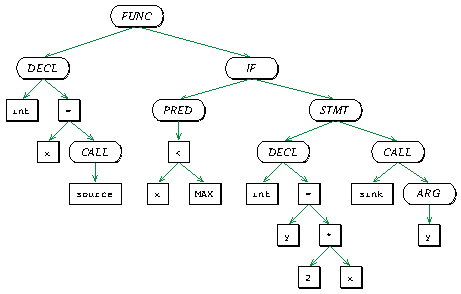
\includegraphics[width=0.75\textwidth]{figures/AST.pdf}
	\caption{The abstract syntax tree for the code in Listing~\ref{listing:cpg}. This figure was taken from~\cite{CPG-yamaguchi2014modeling}.}
	\label{figure:AST}
\end{figure}

A~CFG~\cite{CPG-yamaguchi2014modeling} is an oriented graph describing the possible paths of \textit{program control} and the conditions for their \textit{execution}. The nodes of the graph represent \textit{statements} and \textit{predicates}, while the edges represent \textit{control passing}. Each command node has an outgoing edge labeled~$\varepsilon$, which denotes an \textit{unconditional} passing of control. While a predicate node must have two outgoing edges $true$ and $false$ for different evaluations of a given predicate. Consider the code in Listing~\ref{listing:cpg}. The~CFG constructed for this code is shown in Figure~\ref{figure:CFG-PDG}. The CFG as a property graph is the structure $\mathcal{G}_{\textsc{Cfg}} = ( \mathcal{V}_{\textsc{Cfg}}, \mathcal{E}_{\textsc{Cfg}}, \lambda_{\textsc{Cfg}}, \cdot )$ where $\mathcal{V}_{\textsc{Cfg}}$ is the set of nodes corresponding to the nodes from the AST as follows:

\begin{equation*}
\mathcal{V}_{\textsc{Cfg}} = \{\mathit{v} \in \mathcal{V}_{\textsc{Ast}} \: | \: \mu_{\textsc{Ast}}(v, \textrm'code\textrm') \in \{\textrm'\textsc{Stmt}\textrm', \textrm'\textsc{Pred}\textrm'\} \}
\end{equation*}

The edge labeling function is defined as $\lambda_{\textsc{Cfg}} : \mathcal{E}_{\textsc{Cfg}} \rightarrow \Sigma_{\textsc{Cfg}}$ where the values in the set $\Sigma_{\textsc{Cfg}}~=~\{\textrm'true\textrm',~\textrm'false\textrm',~\textrm'\varepsilon\textrm'\}$ correspond to the meaning of edges in the CFG.

A~PDG~\cite{CPG-yamaguchi2014modeling} is again an oriented graph whose nodes are statements and predicates. There are two types of edges in a PDG, namely \textit{data dependency edges}, which model the influence of a variable on the value of another variable, and \textit{control dependency edges}, which model the influence of predicates on the values of variables. Consider the code in Listing~\ref{listing:cpg}. A~PDG constructed for this code is shown in Figure~\ref{figure:CFG-PDG}. The PDG as a property graph is a structure $\mathcal{G}_{\textsc{Pdg}} = ( \mathcal{V}_{\textsc{Cfg}}, \mathcal{E}_{\textsc{Pdg}}, \lambda_{\textsc{Pdg}}, \mu_{\textsc{Pdg}} )$ where the nodes are the same as in the CFG. The edge labeling function is defined as $\lambda_{\textsc{Pdg}} : \mathcal{E}_{\textsc{Pdg}} \rightarrow \Sigma_{\textsc{Pdg}}$, where the edge labels $\Sigma_{\textsc{Pdg}} = \{\textrm'data\textrm', \textrm'control\textrm'\}$ correspond to the meaning of edges in the PDG. The function assigning attribute values has the form of $\mu_{\textsc{Pdg}}: \mathcal{E_{\textsc{Pdg}}} \bigtimes K_{\textsc{Pdg}} \rightarrow S_{\textsc{Pdg}}$, where $K_{\textsc{Pdg}}~=~\{\textrm'symbol\textrm',~\textrm'condition\textrm'\}$ and $S_{\textsc{Pdg}} = S_{\textsc{Var}} \cup \{\textrm'true\textrm', \textrm'false\textrm'\} $. The set $S_{\textsc{Var}}$ represents the set of names of all variables that occur as the output node of the data dependency edges. The function $\mu_{\textsc{Pdg}}$ then works by assigning the value of the attribute $\textrm'symbol\textrm'$ to the $\textrm'data\textrm'$ edges as the name of the variable represented by the source node of the edge, and $\textrm'control\textrm'$ edges are assigned the attribute value $\textrm'condition\textrm'$ depending on whether they are in the $true$ or $false$ branch. 

\begin{figure*}[t]
  \centering
  \centering
  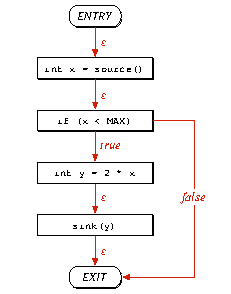
\includegraphics[width=0.36\linewidth]{figures/CFG.pdf}\hfill
  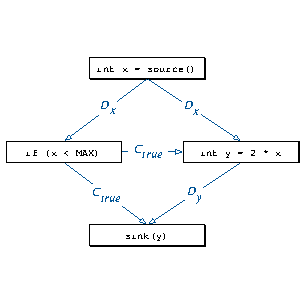
\includegraphics[width=0.48\linewidth]{figures/PDG.pdf}
  \caption{The control flow graph (on the left) and the program dependence graph (on the right) for the code in Listing~\ref{listing:cpg}. These figures were taken from~\cite{CPG-yamaguchi2014modeling}.}
  \label{figure:CFG-PDG}
\end{figure*}

The CPG is then defined using the previous definitions of AST, CFG, and PDG as: 

\begin{equation*}
    \mathcal{G} = ( \mathcal{V}_{\textsc{Ast}}, \mathcal{E}_{\textsc{Ast}} \cup \mathcal{E}_{\textsc{Cfg}} \cup \mathcal{E}_{\textsc{Pdg}}, \lambda, \mu )
\end{equation*}
where the definition of the function $\lambda$ is as follows:

  \begin{equation*}
      \lambda(e) = 
      \begin{cases} 
      \lambda_{\textsc{Ast}} (e) \;\; \textit{if} \;\; e \in \mathcal{E}_{\textsc{Ast}} \\
      \lambda_{\textsc{Cfg}} (e) \;\; \textit{if} \;\; e \in \mathcal{E}_{\textsc{Cfg}} \\
      \lambda_{\textsc{Pdg}} (e) \;\; \textit{if} \;\; e \in \mathcal{E}_{\textsc{Pdg}} 
   \end{cases}
  \end{equation*}

and the definition of the $\mu$ function is:
  
  \begin{equation*}
      \mu(x, p) = 
      \begin{cases} 
      \mu_{\textsc{Ast}} (x, p) \;\; \textit{if} \;\; (x, p) \in \mathcal{V}_{\textsc{Ast}} \bigtimes K_{\textsc{Ast}} \\
      \mu_{\textsc{Pdg}} (x, p) \;\; \textit{if} \;\; (x, p) \in \mathcal{E}_{\textsc{Pdg}} \bigtimes K_{\textsc{Pdg}} \\
   \end{cases}
  \end{equation*}

\iffalse
\begin{multicols}{2}
  \begin{equation*}
      \lambda(e) = 
      \begin{cases} 
      \lambda_{\textsc{Ast}} (e) \;\; \textit{if} \;\; e \in \mathcal{E}_{\textsc{Ast}} \\
      \lambda_{\textsc{Cfg}} (e) \;\; \textit{if} \;\; e \in \mathcal{E}_{\textsc{Cfg}} \\
      \lambda_{\textsc{Pdg}} (e) \;\; \textit{if} \;\; e \in \mathcal{E}_{\textsc{Pdg}} 
   \end{cases}
  \end{equation*}\break
  \begin{equation*}
      \mu(x, p) = 
      \begin{cases} 
      \mu_{\textsc{Ast}} (x, p) \;\; \textit{if} \;\; (x, p) \in \mathcal{V}_{\textsc{Ast}} \bigtimes K_{\textsc{Ast}} \\
      \mu_{\textsc{Pdg}} (x, p) \;\; \textit{if} \;\; (x, p) \in \mathcal{E}_{\textsc{Pdg}} \bigtimes K_{\textsc{Pdg}} \\
   \end{cases}
  \end{equation*}
\end{multicols}
\fi

A~CPG for the code in Listing~\ref{listing:cpg} is shown in Figure~\ref{figure:CPG} where the irrelevant \texttt{FUNC}, \texttt{IF}, and \texttt{STMT} nodes were omitted for demonstration purposes. And also an entry point and an exit point were added.

\begin{figure}[t]
	\centering
	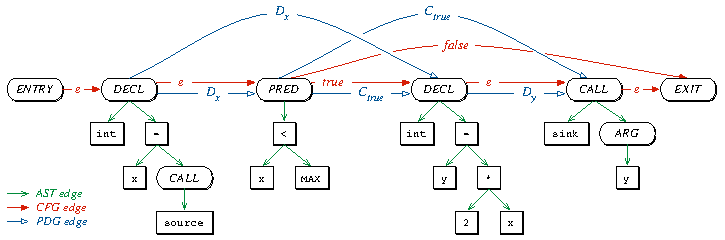
\includegraphics[width=0.98\textwidth]{figures/CPG.pdf}
	\caption{The code property graph for the code in Listing~\ref{listing:cpg}. This figure was taken from~\cite{CPG-yamaguchi2014modeling}.}
	\label{figure:CPG}
\end{figure}

\section{LLVM-Slicer}
\label{slicer}
As described in more detail in Section~\ref{graph-construction-phase}, the LLVM-slicer is used for program slicing in this thesis. LLVM-slicer is an open-source\footnote{\textbf{LLVM-Slicer}' repository: \url{https://github.com/mchalupa/dg}.} tool which uses the DG library~\cite{DG-2-chalupa2020dg, DG-chalupa2020dg}. The DG library implements various interprocedural static analyses -- namely, \textit{pointer analysis}, \textit{data dependence analysis}, \textit{control dependence analysis}, and \textit{value relationship analysis}. These analyses are implemented in DG as independent of the input language. However, the front-end currently supports LLVM bitcode only~\cite{LLVM-bitcode}. LLVM bitcode is a \textit{storage format} for LLVM IR\footnote{\textbf{LLVM Intermediate Representation (LLVM IR)}.}~\cite{LLVM-IR}, which is an \textit{assembly language} used as a low-level representation of code during the various stages of LLVM compilation.

The main use of the DG library is the aforementioned LLVM-slicer, which uses the DG analyses for \textit{program slicing} -- removing pieces of code that have no effect on \textit{user-defined} areas in the code. Results of experiments with LLVM-Slicer on benchmarks from the Software Verification Competition can be found in~\cite{DG-chalupa2020dg}. Although LLVM bitcode is language-independent and can be generated from, e.g., C, C++, or Rust, LLVM-slicer does not support certain constructs in LLVM bitcode that handle \textit{exceptions}. This means that it is not able to handle a C++ program that uses exceptions. If the C++ code is exception-free, it should be able to slice it. The input to the LLVM-slicer is a \textbf{single LLVM bitcode} file and slicing criteria. The output is the sliced LLVM bitcode.

Slicing criteria are specified, for example, using the option \texttt{-sc}. This option allows for a~relatively extensive specification of slicing criteria~\cite{llvm-slicer-readme}. However, in this thesis, the basic format \texttt{-sc file\#function\#line\#obj} is used only. The fields \texttt{file}, \texttt{function}, \texttt{line}, or \texttt{obj} can be empty. The meanings of \texttt{file}, \texttt{function}, and \texttt{line} are straightforward -- they refer to locations in the code. The \texttt{obj} field maps to a function call or a variable use at the location (the code must be compiled with debugging information, see Section~\ref{bitcode-generation}).

Furthermore, it is necessary to define an \textit{entry point function} that must be present in the input bitcode. The default entry point is the \texttt{main} function. However, it can be overridden using the option \texttt{--entry=function}. The entry function acts as the starting point for the analysis -- anything above this function in the call tree is removed.


\section{LLVM2CPG}
\label{llvm2cpg}
In this thesis, the open-source\footnote{\textbf{LLVM2CPG}'s repository: \url{https://github.com/ShiftLeftSecurity/llvm2cpg}.} LLVM2CPG tool is used for generating CPGs from LLVM bitcode, as detailed in Section~\ref{graph-construction-phase}. The CPGs were originally created for high-level languages such as C, which creates some problems when creating CPGs from low-level LLVM IR~\cite{llvm2cpg-webpage}. One problem is mapping LLVM IR instructions to classical high-level operations in order to display the CPG in the same format as, e.g., for the C source code. Some operations can be mapped directly because they have the same \textit{semantics}, others can be modeled using functions, and some cannot be mapped at all and need to be bypassed by another mechanism. The CPG output format can be further processed by Ocular\footnote{\textbf{Ocular}'s documentation: \url{https://docs.shiftleft.io/ocular/quickstart}.} (proprietary), Plume\footnote{\textbf{Plume}'s documentation: \url{https://plume-oss.github.io/plume-docs/}.} (open-source) or Joern (open-source, see Section~\ref{joern}).


\section{Joern}
\label{joern}
Joern is used in this thesis to enrich CPGs with additional information, as detailed in Section~\ref{graph-construction-phase}. Joern~\cite{joern-website} is a powerful open-source\footnote{\textbf{Joern}'s repository: \url{https://github.com/joernio/joern}.} platform providing various tools from the area of static analysis. Using Joern, it is possible to write custom static analyses or \textit{queries} over source files. Joern supports various \textit{programming languages}, such as C, C++, JavaScript, Kotlin, Python, or Java. It is also possible to construct different graph representations of the code (ASTs, CFGs, CDGs, DDGs, PDGs or CPGs), which can be exported in different formats, e.g., DOT~\cite{DOT} or csv for the Neo4j graph database~\cite{neo4j-webpage}. It is also possible to load already constructed CPGs in different formats, e.g., in the output format of the LLVM2CPG tool. Joern can be used as a \textit{command line} tool, through an \textit{interactive environment}, or as an \textit{integration library}.

%%%%%%%%%%%%%%%%%%%%%%%%%%%%%%%%%%%%%%%%%%%%%%%%%%%%%%%%%%%%%%%%%%%%%%%%%%%%%%%

\chapter{D2A Dataset}
\label{chapter-d2a}
This chapter introduces the D2A dataset, which is used in this work to train a system that reduces false positives of the Meta Infer static analyzer. Specifically, the chapter discusses the creation of D2A, the structure of individual samples, comparisons with other existing datasets, and presents statistics regarding the distribution of Meta Infer's error types. This chapter draws primarily from~\cite{D2A-zheng2021d2a, D2A-webpage}.

D2A is a dataset developed by IBM, containing errors found by the Meta Infer static analyzer and information about their validity (true positive/false positive). D2A was first introduced in~\cite{D2A-zheng2021d2a} and is freely available for download at~\cite{D2A-webpage}. The dataset is generated automatically based on \textit{differential static analysis}, and the source files for the D2A generation pipeline are open-source\footnote{\textbf{D2A pipeline}'s repository: \url{https://github.com/IBM/D2A}.}. The dataset fits into the area of static analysis and is primarily intended for creating models aimed at eliminating false reports produced by static analyzers. Initial results from models such as Catboost, LightGBM, Random Forest, Extra-Trees, or the voting model can already be found in the article introducing D2A~\cite{D2A-zheng2021d2a}. The team behind D2A also later published the work~\cite{pujar2024analyzing}, where they improve the existing models and add the C-BERT model, which is \textit{Bidirectional Encoder Representations from Transformers}~\cite{devlin2018bert}, but trained on C code and \textit{fine-tuned} on the D2A dataset for the purpose of classifying reports.

Several reasons led to the selection of the D2A dataset for this thesis:
\begin{enumerate}
    \item It is created from real-world open-source projects.
    \item Meta Infer was used for differential static analysis (thus, samples contain trace, location, error type, etc., which is necessary for extracting slicing information, more information in Section~\ref{graph-construction-phase}).
    \item Being an automatically generated dataset, it is sufficiently large.
    \item The author of this thesis has previously collaborated with the creators of the D2A dataset.
\end{enumerate}

\begin{figure}[t]
	\centering
	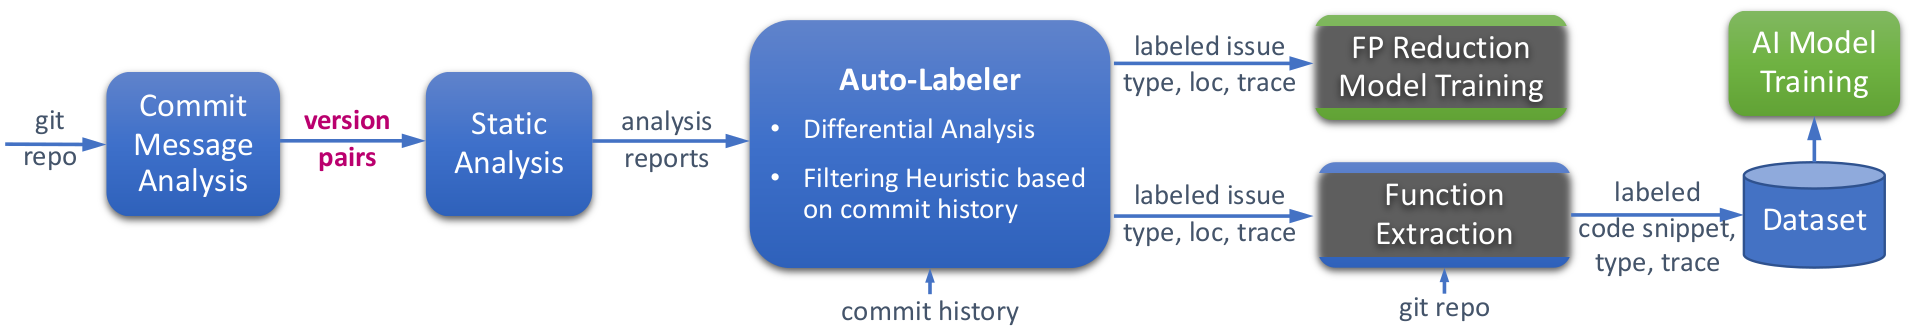
\includegraphics[width=1\textwidth]{figures/d2a-pipeline.png}
	\caption{A~schematic of the D2A generation pipeline. This figure was taken from~\cite{D2A-zheng2021d2a}.}
	\label{figure:d2a-pipeline}
\end{figure}

\subsubsection{Dataset Creation Principle}
The D2A dataset was automatically generated using differential static analysis on open-source projects with extensive git histories. The schematic of the pipeline for generating D2A is shown in Figure~\ref{figure:d2a-pipeline}. The fundamental concept of this pipeline is that the git history includes commits that fix real errors. Therefore, the entire pipeline starts with the identification of these potential fixing commits. These commits are identified using the Commit Message Analyzer, which, through similarity-based methods and key phrase search in commit messages, can select commits that are highly likely fixing errors. For each such commit, Meta Infer (see Section~\ref{infer}) is run on the version of the code before and after the commit. Errors that are found in the before version and are missing in the after version are considered true positives, indicating they have been fixed. For an error to be counted as a true positive, it must also satisfy the following conditions:
\begin{enumerate}
    \item The error must not appear in later versions.
    \item The commit must have modified some part of the bug trace\footnote{A \textbf{bug trace} is information attached to some outputs of Meta Infer. It includes sections of the code that influenced the particular error.} related to the error.
\end{enumerate}

All other errors are considered false positives -- this is, of course, an approximation because otherwise it would imply that the project in its latest version contains no errors, which is highly unlikely. The D2A dataset also includes another type of sample called \textit{after-fix} samples, which are labeled as false positives. Each after-fix sample is generated as a~counterpart to a true positive sample on the after version, where the corresponding true positive have been fixed -- the after-fix samples contain the fixed code. After-fix samples have the property of creating a~balanced dataset along with the true positives and also form pairs that can help models learn to differentiate between true positives and false positives. This is because the pairs provide the models access to the same code with and without the error. However, these samples naturally do not have Meta Infer outputs and are not used in this thesis.

As previously mentioned, each sample includes the output from Meta Infer, the code of the functions related to the error, and additional metadata such as the ID, label, commit hash, and compiler arguments for all files affected by the error (this is possible because Meta Infer needs to compile the code as discussed in Section~\ref{infer}). The complete list of sample attributes is too extensive to be included here, but it is documented in~\cite{d2a-sample-description}. Attributes and their formats necessary for the further explanation will be described in later chapters.

\subsubsection{Comparison with Other Existing Datasets}
There are numerous datasets designed for training models that identify errors in C/C++ code as can be seen in the table comparing existing datasets with D2A in~\cite{D2A-zheng2021d2a}. These datasets are typically categorized into synthetic and real-world types. Synthetic datasets offer the advantage of 100~\% label accuracy and the ability to automatically generate samples, making them sufficiently large. However, synthetic samples are typically simpler and differ from real code, which may lead to poor \textit{generalization} when applied to real-world software. Real-world datasets can be further divided into manually and automatically created. Manually created datasets are highly accurate but are typically too small. Automatically created datasets, on the other hand, suffer from lower accuracy but are large enough. The D2A dataset employs a hybrid approach, automatically generating samples from real-world projects while striving to identify bug-fixing commits that were manually corrected. As a~result, the dataset achieves an accuracy where the true positive class has accuracy of 41~\% and false positive class has accuracy of 81~\%. These accuracies were determined through manual validation of 41 samples labeled as true positive and 16 samples labeled as false positive.

\subsubsection{Dataset Distribution}
The D2A dataset includes 6 open-source projects--openssl\footnote{\textbf{openssl}'s repository: \url{https://github.com/openssl/openssl}.}, libav\footnote{\textbf{libav}'s repository: \url{https://github.com/libav/libav}.}, nginx\footnote{\textbf{nginx}'s repository: \url{https://github.com/nginx/nginx}.}, libtiff\footnote{\textbf{libtiff}'s repository: \url{https://gitlab.com/libtiff/libtiff}.}, httpd\footnote{\textbf{httpd}'s repository: \url{https://github.com/apache/httpd}.}, and FFmpeg\footnote{\textbf{FFmpeg}'s repository: \url{https://github.com/FFmpeg/FFmpeg}.}. While it is theoretically possible to expand it to include any software with a sufficient history of commits, generating it is computationally demanding as it requires running Meta Infer twice for each targeted commit on the entire project. The D2A dataset contains a total of 1,314,276 samples and is provided with a split into \textit{training}, \textit{validation}, and \textit{testing datasets} to match the results of the models from~\cite{D2A-zheng2021d2a, pujar2024analyzing}. Each sample is labeled either true positive (1) or false positive (0) and categorized by error type as determined by Meta Infer outputs, such as \texttt{NULL\_DEREFERENCE}, \texttt{UNINITIALIZED\_VALUE}, etc. Tables~\ref{tab:d2a-bug-types1} and~\ref{tab:d2a-bug-types2} show the counts of samples according to the label, project, and error type. The tables also highlight the types of errors supported by the system for reducing false positives in this thesis, with more details available in Section~\ref{bitcode-generation}.

%%%%%%%%%%%%%%%%%%%%%%%%%%%%%%%%%%%%%%%%%%%%%%%%%%%%%%%%%%%%%%%%%%%%%%%%%%%%%%%

\chapter{Design of a System for Reducing False Positives in Meta Infer}
\label{design}
This chapter describes the design of training and inference pipelines for transforming the D2A dataset into its graphical form, referred to as Graph D2A. Specifically, Section~\ref{training-pipeline} describes the training pipeline, which transforms the D2A dataset into Graph D2A. Section~\ref{bitcode-generation} focuses on the bitcode generation phase, aiming to produce LLVM bitcode from the D2A dataset samples. Section~\ref{graph-construction-phase} explains the creation of extended code property graphs from the generated LLVM bitcode. Section~\ref{graph-d2a} provides a detailed description of the Graph D2A format. Section~\ref{feature-engineering} discusses the feature engineering process, which converts graphs from Graph D2A into an optimized input format for graph neural networks. Section~\ref{gnn-model} outlines how to train graph neural networks using these optimized graphs.

Section~\ref{inference-pipeline} addresses the design of the inference pipeline, a modification of the training pipeline designed to automatically extract graphs and apply the graph neural network models to any real-world C (and a subset of C++) software. Specifically, Section~\ref{capture-phase} describes the capture phase, aimed at running Meta Infer analysis and extracting LLVM bitcode from the build of real-world software. Finally, Section~\ref{inference-phase} discusses the inference phase, which deploys the trained models on the created graphs and ranks a list of errors detected by Infer based on the likelihood of being true positives.

We recall that he goal of this thesis is to create a system to reduce false positives from the static analyzer Meta Infer, described in Section~\ref{infer}. Due to reasons mentioned in Section~\ref{gnn}, graph neural networks (GNNs) were chosen for this task. The goal of the trained models is to rank the errors found by Infer based on their likelihood of being true positives. The D2A dataset was selected for reasons detailed in Chapter~\ref{chapter-d2a}. Although D2A includes the source code of functions mentioned in Infer's bug traces, this information is stored as text (more specifically as JSON) and not as graphs. To enable the training of GNNs on D2A, it first needs to be transformed into an appropriate graph format. According to Section~\ref{cpg}, a suitable and frequently used representation are the code property graphs (CPGs) and its modified versions. The application of GNNs to source code requires a~preliminary mechanism for graph construction. However, the existing graph construction methods have several limitations, which led to the development of our training and inference pipelines. The three main disadvantages of the current solutions are:

\begin{enumerate}
    \item Insufficient graph representations, such as constructing only ASTs~\cite{GNN5-vsikic2022graph}, XFGs~\cite{GNN3-cheng2021deepwukong}, or CFGs~\cite{GNN7-RNN-rabheru2020hybrid}\footnote{This work, however, employs a hybrid approach using both GNN and RNN.}.
    \item Not considering conditional compilation~\cite{GNN1-cao2021bgnn4vd, JOERN-CPG-guan2020code, GNN4-IBM-suneja2020learning, JOERN-CPG-xiaomeng2018cpgva, GNN2-zhou2019devign}.
    \item The inability to automatically construct graphs for any software~\cite{GNN1-cao2021bgnn4vd, JOERN-CPG-guan2020code, GNN4-IBM-suneja2020learning, JOERN-CPG-xiaomeng2018cpgva, GNN2-zhou2019devign}.
\end{enumerate}

Points 2) and 3) are closely linked. The previous works, namely,~\cite{GNN1-cao2021bgnn4vd, JOERN-CPG-guan2020code, GNN4-IBM-suneja2020learning, JOERN-CPG-xiaomeng2018cpgva, GNN2-zhou2019devign}, all use the Joern tool (see Section~\ref{joern}) to construct CPGs (and its various modifications), that is why they are mentioned in both 2) and 3). Although Joern is a very useful tool, its disadvantage is that it analyses the source files directly and is not able to connect to the build process itself. This makes it unable to identify which source files to process and which not to. While Joern can \textit{recursively} find and process source files in a given directory~\cite{joern-doc}, it does indeed process everything it finds in those directories. This becomes a problem if the software includes different versions of the source code, e.g. for different \textit{operating systems} (Windows or Linux), which are selected only during compilation. Joern will thus not be able to correctly construct a CPG without knowing which file to use in a given context. Therefore, Joern cannot be fully automatically deployed on arbitrary software. 

There is a similar problem with conditional compilation where Joern does not know which part of the code to use, or what values the macros have, since they can be (and very often are) defined during compilation. For this reason, Joern considers all macros as undefined by default, and therefore irretrievably loses code fragments that did not satisfy the conditions within \texttt{\#ifdef} or \texttt{\#ifndef} during preprocessing. These problems do not seem to manifest themselves in artificial datasets, and for concrete real-world software, these problems must be solved manually if using pure Joern.

Points 2) and 3) are also closely related to Infer -- since its inputs are compilation commands, and the source code is compiled using them before the analysis (see Section~\ref{infer}) -- Infer analyzes the preprocessed code. This means that the Infer's analysis is platform-dependent -- it can find different errors under various compilation conditions. Therefore, it makes sense to construct graphs from the code as seen by Infer.

The use case of the proposed pipelines differs subtly from previous studies. In particular, we need to construct graphs based on the code in alignment with the Infer report that needs to be sorted. This requires the capability to slice the code according to the information extracted from the report. Program slicing is also employed in some earlier studies. However, in this regard, the most comparable studies, specifically~\cite{D2A-zheng2021d2a, pujar2024analyzing}, do not use program slicing.

The proposed pipelines are intended to create extended CPGs (further discussed in Sections~\ref{graph-d2a} and~\ref{feature-engineering}) from software written in C and a subset of C++. The limitation for C++ arises from the use of LLVM-Slicer, with specific reasons elaborated in Section~\ref{slicer}.


\section{Training Pipeline}
\label{training-pipeline}

\begin{figure}[t]
	\centering
	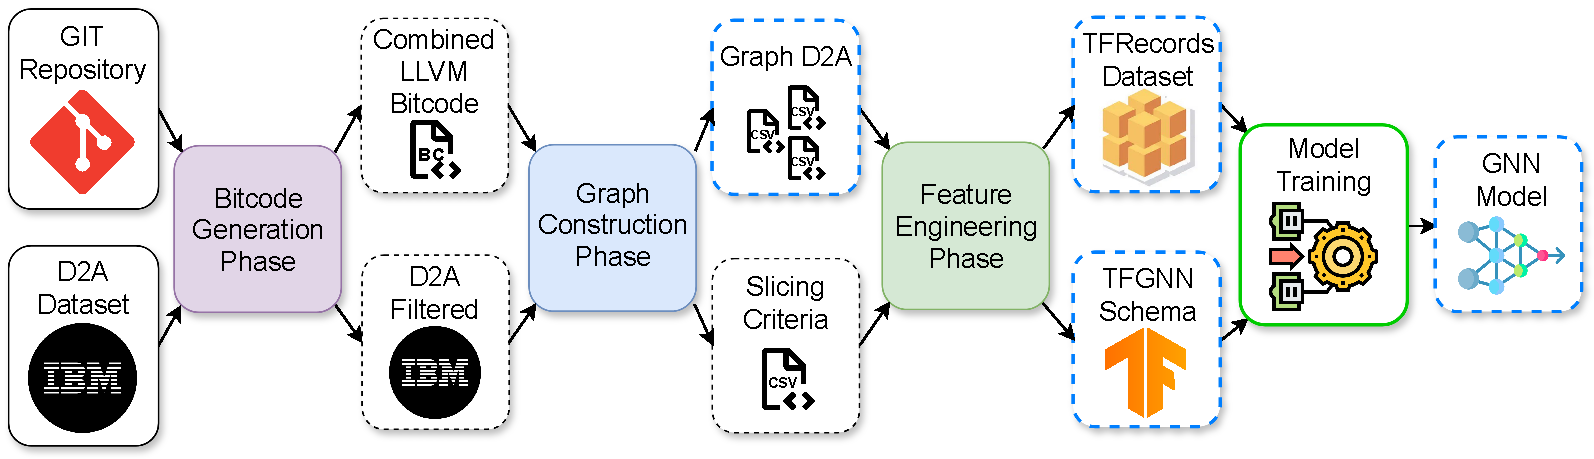
\includegraphics[width=1\textwidth]{figures/training-pipeline.pdf}
	\caption{The figure shows a schematic of the training pipeline that transforms the D2A dataset into Graph D2A, and then trains models on it. Dashed boxes represent the intermediate products and data generated by the pipeline. A~blue outline highlights the important outputs of the pipeline, and a green outline indicates the tool developed in this thesis (in addition to assembling and controlling the entire pipeline). The training pipeline includes phases such as bitcode generation, graph construction, and feature engineering, detailed in Sections~\ref{bitcode-generation},~\ref{graph-construction-phase}, and~\ref{feature-engineering}, respectively. Icons were taken from~\cite{icon-git, icon-ibm, icon-tfrecords, icon-model-training, icon-model}.}
	\label{figure:training-pipeline}
\end{figure}

The goal of the training pipeline is to transform the D2A dataset into its graph version -- Graph D2A, upon which a GNN model will be trained. Figure~\ref{figure:training-pipeline} shows that the training pipeline consists of three stages -- bitcode generation, graph construction, and feature engineering, each detailed in Sections~\ref{bitcode-generation},~\ref{graph-construction-phase}, and~\ref{feature-engineering}, respectively. The input to the entire pipeline is the D2A dataset along with the project repositories from which D2A was generated. The outputs of the pipeline:
\begin{enumerate}
    \item For each project: a \textbf{Graph D2A dataset} -- the D2A dataset transformed into raw extended code property graphs (ECPGs) in the CSV format (see Sectio~\ref{graph-d2a}), which can be used for training GNNs (not only for ranking static analysis reports).
    \item For each project: a \textbf{Graph D2A dataset with feature engineering} (see Section~\ref{feature-engineering}) prepared in the commonly used TFRecords format (again, see Section~\ref{feature-engineering}) for GNN training.
    \item Same for all projects: the \textbf{TFGNN schema} describing the format of the Graph D2A with feature engineering (see Section~\ref{feature-engineering}).
    \item Might be same for all projects (see Chapter~\ref{hyperparameter-tuning}): the \textbf{GNN model} for ranking Infer reports.
\end{enumerate}

Both the training and inference pipelines internally use a conversion to LLVM IR. Since many languages can be compiled into LLVM IR (see Section~\ref{slicer}), the Graph D2A can, to some extent, be considered language-independent; consequently, the models trained on it can also be considered as such. However, it is still important to remember that the original language was C. There are several advantages to generating graphs from LLVM IR:
\begin{itemize}
    \item The output graphs have a simpler structure (as LLVM IR is a much simpler language compared to, for example, C or C++).
    \item The existing tools like LLVM-Slicer and LLVM2CPG can be utilized.
    \item The output graphs are language-independent.
\end{itemize}
However, there are also disadvantages:
\begin{itemize}
    \item The output graphs are larger in terms of the number of nodes and edges.
    \item It is not possible to transform the dataset directly; instead, a recompilation of individual D2A samples is necessary.
\end{itemize}


\subsection{Bitcode Generation}
\label{bitcode-generation}

\begin{figure}[t]
	\centering
	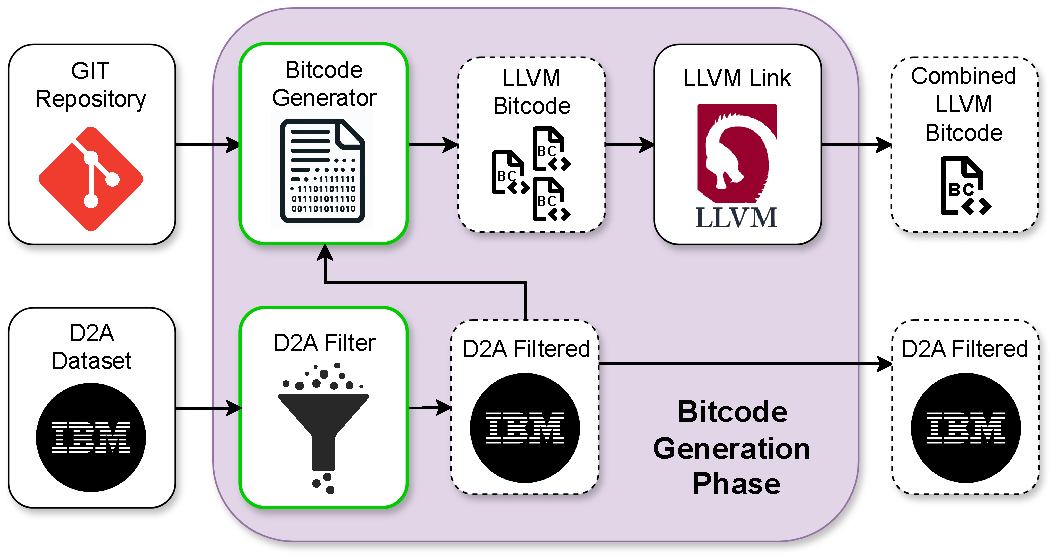
\includegraphics[width=0.8\textwidth]{figures/bitcode-generation.pdf}
	\caption{The figure shows a schematic of the bitcode generation phase,  which generates LLVM bitcode for each D2A sample whose error type is supported. Dashed boxes represent the intermediate products and generated data. A~green outline highlights the tools developed in this thesis. Icons were taken from~\cite{icon-git, icon-ibm, icon-llvm}.}
	\label{figure:bitcode-generation}
\end{figure}

LLVM bitcode is a binary representation of LLVM IR and can be freely converted between the two~\cite{LLVM-bitcode}. For conversion from LLVM IR to LLVM bitcode, the tool \texttt{llvm-as} (llvm assembler) is used, and for the reverse conversion, \texttt{llvm-dis} (llvm disassembler) is employed. However, these tools are not strictly necessary because, as shown in Figure~\ref{figure:bitcode-generation}, the bitcode generator directly produces LLVM bitcode, and all other parts of the pipeline (that work with LLVM IR) operate directly on LLVM bitcode as well.

The objective of the bitcode generator is to produce a set of LLVM bitcode files for each sample from the D2A dataset. The number of LLVM bitcode files for each sample is equal to the number of source files for that sample in D2A. The names of the source files for each sample can be extracted from the \texttt{compiler\_args} attribute in D2A. Each sub-attribute in \texttt{compiler\_args} follows the format~\cite{d2a-sample-description}:

\begin{lstlisting}[language=bash, xleftmargin=2em]
'file.c' : '-compiler\_arg1 -compiler\_arg2 ...'
\end{lstlisting}

Taking only the keys will produce a set of files (for a given sample) that need LLVM bitcode generation.

Before generating LLVM bitcode, it is essential first to filter the dataset and remove samples that will not be transformed. Tables~\ref{tab:d2a-bug-types1} and~\ref{tab:d2a-bug-types2} show that some error types have very few true positives. A~small number of positive samples can make it difficult for models to train as they may not have sufficient information to learn the underlying patterns of true positives for those error types. Consequently, all error types with fewer than \textbf{200 true positives} across the entire dataset will be filtered out. \texttt{DEAD\_STORE} errors are always true positives, as established in previous work by the author~\cite{bc} and also confirmed by the D2A authors' experiments~\cite{D2A-zheng2021d2a} who do not include \texttt{DEAD\_STORE} errors in the manual verification of D2A.

An exception is made for the error types \texttt{BUFFER\_OVERRUN\_L1} and \texttt{INTEGER\_OVERFLOW\_L1}, which are included despite having only 28 and 22 true positives, respectively. The reason is that \texttt{BUFFER\_OVERRUN\_L1} is the same as, for example, \texttt{IBUFFER\_OVERRUN\_L5} -- the only difference being that Infer is more certain of the truthfulness of \texttt{L1} than \texttt{L5} (more information in~\cite{bc}), similarly for \texttt{INTEGER\_OVERFLOW\_L1}. Thus, both errors share the same underlying pattern, and the model should be capable of learning it. In the end, only errors with fewer than 30 true positives are removed, and even out of those, not all are removed, hence the overall data loss is minimal. However, this filtering implies a limitation that the model can only be applied to supported bug types which are highlighted in Tables~\ref{tab:d2a-bug-types1} and~\ref{tab:d2a-bug-types2}.

Generating LLVM bitcode can be accomplished during the compilation using the \texttt{clang} compiler (all projects in D2A are written in C language) of the specified source file by inserting the following options~\cite{clang-doc} (which were recommended by the old version of Joern documentation\footnote{Joern's old documentation (unavailable): \url{https://docs.joern.io/llvm2cpg/getting-bitcode}.}, which unfortunately is no longer available) into the compilation command:

\begin{enumerate}
    \item \texttt{-emit-llvm} -- ensures that LLVM bitcode is used for \textit{object files}.
    \item \texttt{-g} -- adds debug information which allows \textit{backward mapping} of LLVM bitcode to the original source code, enabling the use of program slicing based on location information~\cite{llvm-slicer-readme}.
    \item \texttt{-grecord-command-line} -- inserts more debug information into the LLVM bitcode.
    \item \texttt{-fno-inline-functions} -- disables the use of \textit{inline functions}.
    \item \texttt{-fno-builtin} -- prevents the compiler from inserting \textit{built-in functions}.
\end{enumerate}

The compilation command must indeed be specifically for compiling (it must include \texttt{-c}), and not for linking, preprocessing, etc. Additionally, the \texttt{-o} option along with its value must be removed, so that the compilation command generates a \texttt{.bc} (LLVM bitcode) file instead of the original file. The \texttt{compiler\_args} attribute contains only options -- typically just \texttt{-I} (include directories) and \texttt{-D} (definitions of macros and their values). Since neither \texttt{-c}, \texttt{-o}, nor the specific compiler used are mentioned among the options, it is unnecessary to remove \texttt{-o} or check if it is indeed a compilation command. Instead of the originally used compiler (which cannot be identified from D2A alone), \texttt{clang} will be used. Given that Infer also internally uses \texttt{clang} (see Section~\ref{infer}), it ensures that both compilations -- for analysis and for bitcode generation -- are identical (different compilers might apply different optimizations and have different default behavior). The resulting compilation command for the file \texttt{file.c}, generating \texttt{file.bc}, would look like this:

\begin{lstlisting}[language=bash, xleftmargin=2em]
clang -emit-llvm -g -grecord-command-line -fno-inline-functions \
-fno-builtin {D2A_compiler_args} -c file.c
\end{lstlisting}

Thanks to this compilation process and the information from \texttt{compiler\_args}, the definition and application of macros are successfully achieved. This addresses the previously unconsidered problem of conditional compilation, which was mentioned at the beginning of this chapter.

At this stage, the use of the inference pipeline, described in more detail in Section~\ref{inference-pipeline}, might seem applicable. It is capable of generating LLVM bitcode for any C/C++ project. However, D2A consists of 6 projects, and within a single project, the samples are not made from the same version, but from thousands of different versions of the given project. The inference pipeline would thus need to be executed separately for each of these versions, which is computationally infeasible. The generated LLVM bitcode for each sample would be vast, and most of it would later be removed during program slicing. Instead, information from D2A and the git repositories of projects from D2A is used to compile only the necessary files on specific project versions.

For simplicity, consider the transformation of a single project within D2A. For each sample, it is necessary to restore the project repository to the version (commit) in which the error appears, which can be obtained from the D2A attribute \texttt{commit}. Then, the names of the files that need to be transformed into LLVM bitcode are extracted from D2A. These files are then compiled to generate LLVM bitcode. However, for this process to be fully automated, successful compilation of at least the required files across all required commits must be ensured. Proper configuration data, all dependencies, generated data (e.g., C headers), etc., are needed for successful compilation. All these elements change with software development, and automating LLVM bitcode generation requires manual adjustment to the specific project (more in Section~\ref{implementation-bitcode-generator}).

Once a set of LLVM bitcode files is generated for each sample, these files need to be merged into a single one. This requirement stems from the requirements of the LLVM-Slicer tool (see Section~\ref{slicer}). The tool \texttt{llvm-link}~\cite{llvm-link-doc} is used for this purpose, which, despite its name, is not involved in the typical linking process of compilers. \texttt{llvm-link} merely combines multiple LLVM bitcode files into a single one while preserving the LLVM bitcode format. The tool \texttt{llvm-link} was chosen based on recommendations in the documentation of the LLVM-Slicer tool~\cite{llvm-slicer-readme}. The output of the bitcode generation phase is, for each sample in the dataset, a single LLVM bitcode file containing the transformed source code of all files relevant to that sample. Additionally, the D2A dataset is filtered to include only supported error types.


\subsection{Graph Construction}
\label{graph-construction-phase}
The input to the graph construction phase, as shown in Figure~\ref{figure:graph-construction}, consists of the filtered D2A dataset and an LLVM bitcode file for each sample. The output for each sample is a~CPG, extended with additional information (the format of the output data is described in Section~\ref{graph-d2a}). The output graphs are stored in the CSV format for the Neo4j database. Additionally, a script in the Cypher language is included with each sample to load the respective graph into the database~\cite{joern-doc}. Although Neo4j is commonly used for storing and querying graph data, it is not used in this thesis.

\begin{figure}[t]
	\centering
	\includegraphics[width=1\textwidth]{figures/graph-construction.png}
	\caption{The figure shows a schematic of the graph construction phase, which creates a~raw ECPG for each input D2A sample. Dashed lines represent the intermediate products and generated data. A~green outline highlights the tools developed in this thesis. Icons were taken from~\cite{icon-ibm, icon-funnel, icon-shiftleft, icon-graph, joern-website}.}
	\label{figure:graph-construction}
\end{figure}

\subsubsection{Program Slicing}
First, for each sample, it is necessary to extract information required for program slicing performed by the LLVM-Slicer (see Section~\ref{slicer}) from the D2A dataset. This information includes:
\begin{itemize}
    \item The \textbf{entry point function} -- the function in which the program slicing should start (the top-most function in the bug trace).
    \item The \textbf{file} -- the name of the file where the error is located.
    \item The \textbf{function} -- the name of the function in which the error is located.
    \item The \textbf{line} -- the line number on which the error is located.
    \item The \textbf{variable} (optional) -- the variable related to the error (relevant only for certain types of errors).
\end{itemize}

These details form the so-called slicing criteria. The challenge with extracting slicing criteria is that each type of error has a different format, and these details cannot be uniformly obtained from all samples. The name of the entry point function is an exception and can be retrieved for all samples from the \texttt{procedure} attribute (both from D2A and Infer analysis output). The entry function is the highest-level function in the call graph\footnote{A \textbf{Call Graph} is an oriented graph in which nodes represent functions and edges represent calls between these functions. It can be considered a substructure of the control flow graph to some extent.} among all the functions mentioned in the Infer bug trace. Practically, this means that anything above this function is not important for the manifestation of the error. If the entry function itself is called with the correct parameters and in the right context, it must lead to the reported error (assuming it is a true positive). This is crucial information for program slicing, as it means that everything above the entry function can be discarded (which is exactly what LLVM-Slicer does), because it is not useful for the future classification of true positives/false positives.

In total, 14 types of errors are supported, as shown in Tables~\ref{tab:d2a-bug-types1} and~\ref{tab:d2a-bug-types2}. However, some error types are similar enough that slicing criteria can be extracted in the same way, resulting in the following groups:
\begin{enumerate}
    \item \texttt{NULLPTR\_DEREFERENCE} -- this group contains only the identically named type.
    \item \texttt{INTEGER\_OVERFLOW} -- includes all \texttt{INTEGER\_OVERFLOW\_}\textbf{X} where $X \in \{\texttt{L1}, \texttt{L2}, \texttt{L5}, \texttt{U5}\}$.
    \item \texttt{INFERBO\_ALLOC\_MAY\_BE\_BIG} -- contains only the identically named type.
    \item \texttt{UNINITIALIZED\_VALUE} -- again contains only the identically named type.
    \item \texttt{BUFFER\_OVERRUN} -- includes all \texttt{BUFFER\_OVERRUN\_}\textbf{X} where 
    \newline
    $X~\in~\{\texttt{L1}, \texttt{L2}, \texttt{L3}, \texttt{L4}, \texttt{L5}, \texttt{U5}\}$.
    \item \texttt{NULL\_DEREFERENCE} -- the last group contains only the identically named type.
\end{enumerate}

\paragraph{The \texttt{NULLPTR\_DEREFERENCE} Group}
For errors of type \texttt{NULLPTR\_DEREFERENCE}, three different formats of the Infer output were found in the D2A, distinguishable by the \texttt{qualifier} attribute~\cite{d2a-sample-description}, which contains a~brief description of the error and shares the same name as in the JSON output of Infer:
\begin{enumerate}
    \item \texttt{'call to `put\_bits()` eventually accesses memory that is the null 
    \newline
    pointer on line 543 indirectly during the call to `init\_put\_bits()`.'}
    \newline
    -- e.g., sample with \texttt{id: ffmpeg\_8e48b53d696b53cef2814548e4d0693387e875ea\_1}.
    \item \texttt{'accessing memory that is the null pointer on line 3191 indirectly 
    \newline
    during the call to `av\_malloc()`.'} 
    \newline
    -- e.g., sample with \texttt{id: ffmpeg\_6a30264054cc320fe610c072c71d008f7e3c3efb\_1}.
    \item \texttt{'accessing memory that is the null pointer on line 315.'}
    \newline
    -- e.g., sample with \texttt{id: ffmpeg\_9c908a4c99e0498dd26bd1de84ff085ac8e73e4a\_1}.
\end{enumerate}

For Cases 2) and 3), the \texttt{file}, \texttt{function}, and \texttt{line} information in the \texttt{bug\_info} attribute are correct~\cite{d2a-sample-description}. However, for Case 1), the same information only contains the location of the function call where the dereference occurs -- in this case, \texttt{put\_bits()}. The correct error location needs to be obtained from the last step of the \texttt{trace} attribute (bug trace), as shown in Listing~\ref{listing:nullptr-dereference-trace} which shows this last step for Case 1). For Cases 2) and 3), the locations in the \texttt{bug\_info} and the last \texttt{trace} step coincide, thus uniformly extracting information from the last bug trace step is feasible for all three formats. Additionally, all three formats share the same last step with \texttt{description} -- \texttt{invalid access occurs here}. The only difference is that in \texttt{trace}, \texttt{function} is named as \texttt{func\_name} and \texttt{line} must be extracted from \texttt{loc}, as seen in Listing~\ref{listing:nullptr-dereference-trace}.

\begin{lstlisting}[
    language=json, 
    label={listing:nullptr-dereference-trace}, 
    float=t,
    caption={The last step of the \texttt{trace}~\cite{d2a-sample-description} for a \texttt{NULLPTR\_DEREFERENCE} error taken from the sample with \texttt{id: ffmpeg\_8e48b53d696b53cef2814548e4d0693387e875ea\_1} on the FFmpeg project. The listing demonstrates the format of storing a bug trace in D2A.}
]
 "trace": [
     // ... other trace steps ...
     {
         "idx": 16,
         "level": 2,
         "description": "invalid access occurs here",
         "func_removed": null,
         "file_removed": null,
         "file": "libavcodec/put_bits.h",
         "loc": "179:9",
         "func_name": "put_bits",
         "func_key": "libavcodec/put_bits.h@139:1-189:2",
         "is_func_definition": true,
         "url": "https://github.com/FFmpeg/FFmpeg/blob/5962f6b0da037da30 fcc848331afa6a081a4eb09/libavcodec/put_bits.h/#L179"
     }
    ]
\end{lstlisting}

For \texttt{NULLPTR\_DEREFERENCE} errors, it is indeed sensible to consider extracting the variable name because null dereferences typically occur on a variable. However, they can theoretically occur on a constant like \texttt{(NULL)} or a general expression, such as \texttt{(p-p)}. When the null dereference occurs on a variable, it would be best to extract the name of this variable along with the error location. A~more precise slicing criterion would allow for more accurate program slicing, thereby removing more unnecessary information from future graphs. Unfortunately, the variable name does not appear in any of the described formats of \texttt{NULLPTR\_DEREFERENCE} in the Infer output (and thus not in D2A either). The only clue available is the column, which can be extracted from the \texttt{loc} attribute (see Listing~\ref{listing:nullptr-dereference-trace}). Knowing the line and column where the dereference occurs might seem to simplify the extraction of the variable name. However, it is necessary to distinguish when the dereference is on a variable, a constant, an expression, or a macro. Distinguishing a variable can be done straightforwardly using the C language naming rules for variables -- a name can only follow the pattern \texttt{[a-zA-Z\_][a-zA-Z0-9\_]*}, and anything else cannot be a variable and thus should not be extracted. However, macros can be named the same as variables (and typically are). Therefore, distinguishing between a variable and a macro is non-trivial and would require at least preprocessing by a compiler and subsequent adjustment of the error position, as macro expansion can change both the line and column. For now, the extraction of the variable name for \texttt{NULLPTR\_DEREFERENCE} will be left for future improvements.

\paragraph{The \texttt{INTEGER\_OVERFLOW} Group}
For the \texttt{INTEGER\_OVERFLOW} error types, two formats were identified, which can again be distinguished using the \texttt{qualifier} attribute:
\begin{enumerate}
    \item \texttt{([0, 8] - [0, 8]):unsigned32.} 
    \newline
    -- e.g., sample with \texttt{id: ffmpeg\_1542087b54ddf682fb6177f999c6f9f79bd5613f\_1}.
    \item \texttt{([0, 1] - 1):unsigned32 \textbf{by call to} `avfilter\_unref\_buffer`.} 
    \newline
    -- e.g., sample with \texttt{id: ffmpeg\_ca5973f0bfac4560342605f8a52efc88b4f4dbd3\_1}.
\end{enumerate}
For Case 1), location information can be obtained directly from \texttt{bug\_info}. For Case 2), a~similar problem arises as with \texttt{NULLPTR\_DEREFERENCE} Case 1) -- \texttt{bug\_info} contains only the location of the function call, in this case, \texttt{avfilter\_unref\_buffer}, where the integer overflow/underflow occurs. It is necessary to extract information from the \texttt{trace} attribute. To cause an overflow/underflow, two operands are needed (with the exception of operators like \texttt{++}, which in terms of value change is equivalent to \texttt{+1}), and each operand can either be a variable or an expression. Although LLVM-Slicer is capable of slicing based on multiple criteria (in this case, both operands), to ensure the resulting graph is complete, it is necessary to include the operation itself. Thus, slicing must be based on the entire line, as slicing by expression is not yet supported (to the best of the author's knowledge).

\paragraph{The \texttt{INFERBO\_ALLOC\_MAY\_BE\_BIG} Group}
The \texttt{INFERBO\_ALLOC\_MAY\_BE\_BIG} group contains only a single error type of the same name, and only one format was identified:
\begin{enumerate}
    \item \texttt{Length: [0, 2147483631] \textbf{by call to} `av\_dup\_packet`.}
    \newline
    -- e.g., sample with \texttt{id: ffmpeg\_c36d9fb10c31c6835d01232fddff6932a3ce347f\_1}.
\end{enumerate}

Similar to \texttt{NULLPTR\_DEREFERENCE} Case 1), it is necessary to extract the location from the last step of the \texttt{trace} because the \texttt{bug\_info} points to a function call in which the error occurs, in this case, \texttt{av\_dup\_packet}. The correct location points to a function call that allocates memory, such as \texttt{malloc}, \texttt{realloc}, etc. If the call appears as \texttt{realloc(ptr, size)}, ideally, it is preferable to slice directly by \texttt{size} because its value is of interest. However, the call can often appear as \texttt{realloc(ptr, str\_len + 1)}, and in this case, the value of the entire expression is needed. Of course, it is possible to extract the name of the variable only in certain cases, but there are still the previously mentioned issues with macros and also with detecting the correct argument. From the output of Infer, it is not possible to determine which argument it concerns. With functions like \texttt{malloc} or \texttt{realloc}, the argument is known from their definitions, but it is necessary to consider cases where, during Infer analysis, custom models are created, and theoretically, any function could be considered an allocation function. For these reasons, for this type of error, slicing is only done by the line. Moreover, allocation functions typically are not very large, so including their code in the graphs does not represent too much unnecessary data.

\paragraph{The \texttt{UNINITIALIZED\_VALUE} Group}
The \texttt{UNINITIALIZED\_VALUE} group also contains only a single error type of the same name. Two formats have been identified, which can again be distinguished using the \texttt{qualifier} attribute:
\begin{enumerate}
    \item \texttt{The value read from ret was never initialized.} 
    \newline
    -- e.g., sample with \texttt{id: ffmpeg\_ed80423e6bcfe18cca832b74dcc877427f8cf346\_1}.
    \item \texttt{The value read from pix[\_] was never initialized.}
    \newline
    -- e.g., sample with \texttt{id: ffmpeg\_1f62bae77d6ced3b79deaa8ce5ba3381fd4a541d\_1}.
\end{enumerate}
Neither format includes additional information in the \texttt{trace}, so the information is solely from \texttt{bug\_info}. The location is correct for both formats. Case 1) concerns uninitialized variables, where it makes sense to slice also by the variable because the specific variable itself is of interest. Moreover, the variable's name can be easily obtained from the \texttt{qualifier}. Case 2) concerns uninitialized arrays (or items in an array), where the situation is more complex because it is not possible to obtain the access index into the array from the Infer output. It could be extracted from the code, but problems such as slicing by expressions and macros arise. If slicing is done only by the line, then information about the index would be included in the output. However, experience from checking outputs from Infer (especially in~\cite{bc}) suggests that if an array item is uninitialized, it is because the entire array was not initialized. For these reasons, even for Case 2), the variable name is extracted -- in this case, it is always an array, and the slicing is done with respect to the array.

\paragraph{The \texttt{BUFFER\_OVERRUN} Group}
For the \texttt{BUFFER\_OVERRUN} error types, two formats have been identified, which can again be distinguished using the \texttt{qualifier} attribute:
\begin{enumerate}
    \item \texttt{Offset: [0, 15] Size: 4.}
    \newline
    -- e.g., sample with \texttt{id: ffmpeg\_61d490455ade68a02dfdcfdb172ba3ded2fe0f9d\_1}.
    \item \texttt{Offset: [1, 4] Size: 4 by call to `filter\_mb\_mbaff\_edgecv`.} 
    \newline
    -- e.g., sample with \texttt{id: ffmpeg\_0f5e5ecc888af015015f2ce1211a066350fbe377\_1}.
\end{enumerate}
For Case 1), the information in \texttt{bug\_info} is correct. For Case 2), the location needs to be taken from the last step of the \texttt{trace} again. Neither format in the Infer output specifies the name of the array or the index name (if it involves a variable rather than an expression). For these types of errors, both the name of the array and the index are necessarily required. To obtain both names, a more complex extraction method from the source code would again be necessary. Hence, for this type of error, slicing is currently done by the line.

\paragraph{The \texttt{NULL\_DEREFERENCE} Group}
The \texttt{NULL\_DEREFERENCE} group contains only a single error type of the identical name. \texttt{NULL\_DEREFERENCE} and \texttt{NULLPTR\_DEREFERENCE} are semantically identical, with the difference lying in the Infer plugin that produced them -- Bi-abduction (\texttt{NULL\_DEREFERENCE}) and Pulse (\texttt{NULLPTR\_DEREFERENCE}). Since they originate from different plugins (which may have issues with different language constructs leading to varying patterns of true and false positives) and also have different formats, it makes sense to list them separately. Two formats have been found, distinguishable by the \texttt{qualifier} attribute:

\begin{enumerate}
    \item \texttt{pointer `filter` last assigned on line 3191 could be null and is
    \newline
    dereferenced at line 3194, column 9.}
    \newline
    -- e.g., sample with \texttt{id: ffmpeg\_15ae526d6763d8e21833feb78680ee3571080017\_1}.
    \item \texttt{pointer `null` is dereferenced by call to `ff\_sdp\_write\_media()` at
    \newline
    line 2538, column 5.}
    \newline
    -- e.g., sample with \texttt{id: ffmpeg\_a94ada4250ff1d9e6101c910fe71dde6c3b5e485\_1}.
\end{enumerate}

Ideally, for this type of error, it would be desirable to slice by the variable name (if the incorrect dereference occurs on a variable). For Case 1), both the location information and the variable name can be obtained directly from \texttt{bug\_info}, as the variable name is mentioned in the \texttt{qualifier}. For Case 2), \texttt{bug\_info} contains only the location of the function call within which the incorrect dereference occurs. If the \texttt{qualifier} in Case 2) contains a variable name (instead of \texttt{null}), it is not the variable on which the dereference occurs but a variable whose value is passed to the called function. Unfortunately, in the \texttt{trace}, it is not possible to determine which step represents the incorrect dereference because most steps lack a \texttt{description}. In some cases, the last step in \texttt{trace} represents the incorrect dereference, but in some others, it does not. Unfortunately, it is also not possible to distinguish between these types. For these reasons, for Case 2), slicing is done only by the line of the called function. This ensures that the error is included in the graph, even if it is deeper in the call graph. However, this introduces a significant ammount of unnecessary information.

\paragraph{The \texttt{adjusted\_bug\_loc} Attribute}
An important note is that any sample, regardless of the type of error, may contain the \texttt{adjusted\_bug\_loc} attribute in D2A. The attribute adjusts the location of the error if the \texttt{bug\_info} -- extracted directly from Infer's output -- does not precisely pinpoint the error's location. The \texttt{adjusted\_bug\_loc} was derived using the same principles previously described for each group of error types. This raises the question of why not directly use \texttt{adjusted\_bug\_loc}. In the training pipeline, it is indeed possible to use these data, but in the inference pipeline, this information is no longer available because it only operates with Infer's output on real-world software, not with D2A. Therefore, a similar method of extracting precise error locations from the Infer report will eventually need to be designed and implemented for real-world applications. Utilizing it also in the training pipeline has additionally allowed verification of whether the author of this thesis and the authors of D2A agree on the method for extracting the exact location of errors -- this has been verified across all samples of supported error types.

\paragraph{The Application of Program Slicing}
The extracted slicing criteria, along with LLVM bitcode, form the input for LLVM-Slicer (see Section~\ref{slicer}). The output is a sliced LLVM bitcode according to the input slicing criteria. The purpose of program slicing is to remove parts of the graphs that do not influence the occurrence of the error. Consequently, this effectively reduces the size of the resulting graph and eliminates unnecessary information, which should facilitate and speed up the learning process for GNN models. LLVM-Slicer was chosen based on a recommendation by Ing. Viktor Malík. Upon verification, it was found to meet all the requirements, particularly in terms of input and output formats. An alternative, such as the tool \texttt{llvm-slicing}\footnote{\textbf{llvm-slicing}'s repository: \url{https://github.com/zhangyz/llvm-slicing}.}, is no longer maintained.

Program slicing at this stage of the pipeline also allows for specifying slicing criteria in relation to the original code, which is more appropriate than specifying them later in the CPG and slicing using tools like Joern~\cite{joern-doc}. Theoretically, it should be possible to identify slicing criteria in the output CPG graph thanks to debug information (see Section~\ref{bitcode-generation}) attached to individual nodes, which can map certain LLVM constructions back to the original code. However, this information may be lost during CPG construction, as discussed in Section~\ref{llvm2cpg}. Consequently, it becomes challenging to accurately map CPG nodes back to the original code, risking the incorrect construction of the node set intended for slicing criteria.

\subsubsection{Generation of Extended Code Property Graphs from LLVM Bitcode}
Sliced LLVM bitcode serves as the input to the LLVM2CPG tool (see Section~\ref{llvm2cpg}), which generates CPGs. These CPGs are then processed by the Joern tool (see Section~\ref{joern}), whose task is to:

\begin{enumerate}
    \item convert CPGs from binary to the CSV format,
    \item create Extended CPGs (ECPGs) by adding additional layers such as information about types, files, functions, and more (see Section~\ref{graph-d2a}).
\end{enumerate}

Joern is utilized solely as a CLI\footnote{\textbf{Command Line Interface (CLI)}.} tool in this thesis. It takes a binary CPG and a script with a list of commands to execute, primarily load and save operations, as Joern automatically constructs additional layers upon loading. The resulting ECPGs are saved again in a binary format. The final step involves converting the binary format into the easily usable CSV format using a Joern sub-tool -- \texttt{joern-export}~\cite{joern-doc}, which creates a directory with CSV files containing:
\begin{itemize}
    \item CSV header file,
    \item CSV data file (without header),
    \item Cypher script for importing into the Neo4j database.
\end{itemize}

The CSV header file is kept for each sample, even though it might seem unnecessary. The reason lies in Joern's non-deterministic behavior regarding the columns generated on different machines. For instance, the header for \texttt{METHOD} nodes (see Section~\ref{graph-d2a}) in httpd (true positives) and openssl (true positives) -- openssl has two additional columns, which, however, contain no useful information.

The Joern tools (and Joern Export) were chosen due to their frequent use in the field of GNNs~\cite{GNN1-cao2021bgnn4vd, JOERN-CPG-guan2020code, GNN4-IBM-suneja2020learning, JOERN-CPG-xiaomeng2018cpgva, GNN2-zhou2019devign}. LLVM2CPG is specifically recommended on the LLVM Project website for generating CPGs in combination with Joern~\cite{llvm2cpg-webpage}.

\subsection{Graph D2A}
\label{graph-d2a}
The D2A dataset, where each sample is transformed into an ECPG generated using the Joern tool, will henceforth be referred to as \textbf{Graph D2A}. Graph D2A is one of the main contributions of this thesis and, in combination with the original D2A, enables other researchers to create their own graph representations (based on CPGs) for GNNs and apply their own feature engineering. As mentioned earlier, ECPGs contain additional information compared to CPGs described in Section~\ref{cpg}. Additionally, the CSV format facilitates further preprocessing of the dataset before inputting into GNNs. In this thesis, individual samples of Graph D2A will be referred to as raw ECPGs, precisely because they are in the CSV format and because the node/edge attributes are not yet processed or modified -- they often lack, have an inappropriate format, and the format is not uniform (\texttt{int}, \texttt{float}, \texttt{string}, etc.). Processing raw ECPGs into a format suitable for training GNNs will be addressed in Section~\ref{feature-engineering}.

The complete output format of raw ECPGs is described in the automatically generated documentation of the Joern tool~\cite{joern-cpg-doc} (version 1.1), from which the following information is also taken. Like CPGs, raw ECPGs are directed, node-labeled, edge-labeled, multigraphs. The set of nodes that share the same label will be referred to as a \textit{node set}, for future compatibility. All nodes within a single node set have the same set of attributes (although some values may be missing). Similarly, edges that share the same label will be referred to as an \textit{edge set}. No edge sets (except \texttt{REACHING\_DEF}) in raw ECPGs have attributes, but as mentioned in the following sections, it may make sense to move certain attributes from nodes to edges. Raw ECPGs consist of \textit{layers}, where each layer can add additional node/edge sets or their attributes. Individual layers may be language-dependent, as Joern can generate ECPG graphs from any language for which a frontend is written. Currently, this includes languages such as \textbf{LLVM IR}, C/C++/C\#, Java, JavaScript, Python, Kotlin, PHP, Go, Ruby, Swift, and more~\cite{joern-cpg-doc, joern-doc}. The Joern layers that are \textbf{completely} missing for LLVM IR are the \textbf{Comment Layer}, \textbf{Finding Layer}, \textbf{TagsAndLocation Layer}, \textbf{Configuration Layer}, \textbf{Binding Layer}, and \textbf{Annotation Layer}. These missing layers will not be further described.

Since this thesis utilizes only LLVM IR (specifically LLVM bitcode) as Joern input, the following explanation includes only layers generated for LLVM IR. Although the Joern documentation is highly detailed, it does not describe all the attributes of the node sets. A~complete list of these attributes is provided in Table~\ref{tab:attributes1}. The description of each attribute is discussed in detail in Section~\ref{feature-engineering}, where the removal of irrelevant attributes is addressed. Node sets are hierarchically organized -- if node set \texttt{X} inherits from node set \texttt{Y}, it implies that \texttt{X} contains the same attributes as \texttt{Y} and adds some unique ones (typically). A~visualization of the hierarchy of node sets (which are generated for LLVM bitcode) and base class node sets can be seen in Figure~\ref{figure:node-set-hierarchy}.

\begin{figure}[t]
	\centering
	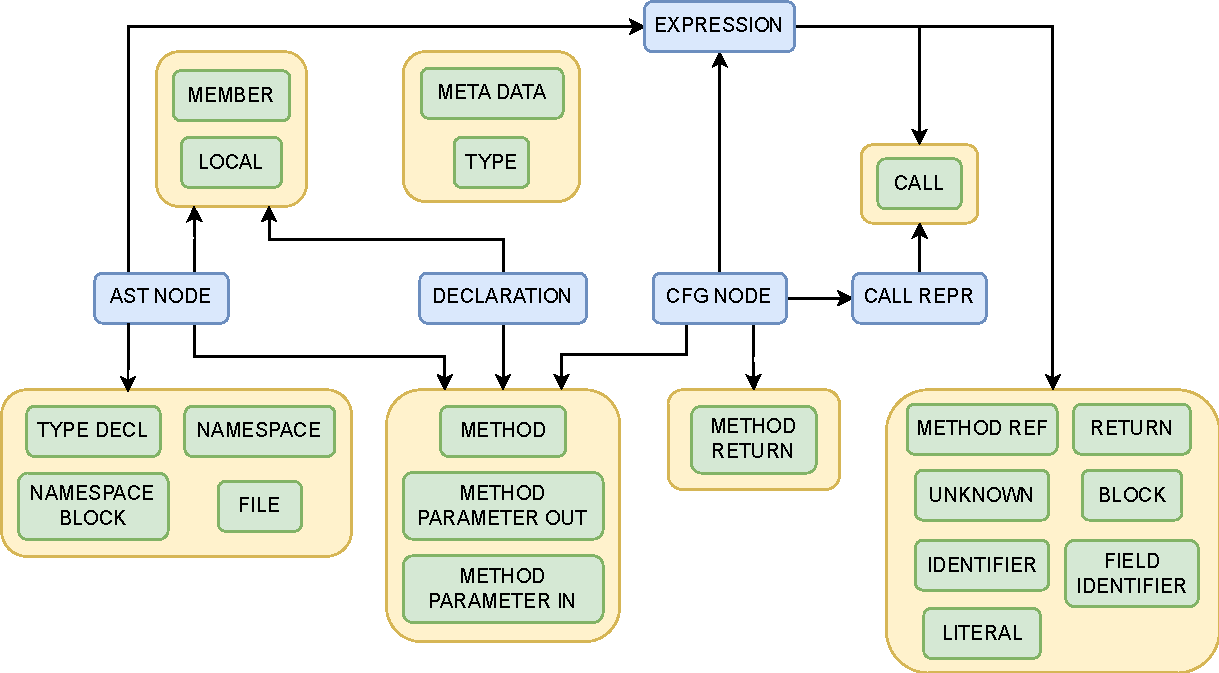
\includegraphics[width=1\textwidth]{figures/node-set-hierarchy.pdf}
	\caption{The figure shows the hierarchy of node sets in green (generated for LLVM IR) and the base class node sets in blue.}
	\label{figure:node-set-hierarchy}
\end{figure}

\textbf{The MetaData Layer} contains only one node set -- \texttt{META\_DATA}. In each graph, there is precisely one such node with \texttt{ID: 1}, containing information about how the graph was generated -- e.g., input language, version, etc.

\textbf{The FileSystem Layer} includes information about the files from which the graph was generated. It specifically adds the node set \texttt{FILE}, where each node represents an input source file. This layer also introduces an edge set \texttt{SOURCE\_FILE}, which connects nodes from other node sets to \texttt{FILE} nodes based on their source file.

\textbf{The Namespace Layer} introduces the \texttt{NAMESPACE} node set, which resembles \texttt{FILE} and describes the namespace as known from programming. This layer also introduces the \texttt{NAMESPACE\_BLOCK} node set, which groups code under a common namespace, defined using specific statements like \texttt{namespace{ }} in C++ or \texttt{package} in Java.

\textbf{The Method Layer} includes declarations of methods, functions, and procedures (collectively referred to as 'functions' hereafter). This layer also includes their inputs and outputs but \textbf{does not contain their code}. Included in this layer are node sets:
\begin{itemize}
    \item \texttt{METHOD} -- information about a specific function.
    \item \texttt{METHOD\_PARAMETER\_IN} -- represents the input parameters of a specific \texttt{METHOD} node.
    \item \texttt{METHOD\_PARAMETER\_OUT} -- represents the output parameters corresponding to the inputs of a specific \texttt{METHOD} node.
    \item \texttt{METHOD\_RETURN} -- represents the return parameter of a specific \texttt{METHOD} node.
\end{itemize}

\textbf{The Type Layer} contains information about type declarations, type relationships, type instantiation, type hierarchies, parameterized types, and aliases. This layer introduces the following node sets:
\begin{itemize}
    \item \texttt{MEMBER} -- member of a structured type.
    \item \texttt{TYPE} -- instance of a type.
    \item \texttt{TYPE\_ARGUMENT} -- argument used during parameterized type instantiation (e.g., Java \texttt{Generics}, C++ \texttt{templates}).
    \item \texttt{TYPE\_DECL} -- type declaration.
    \item \texttt{TYPE\_PARAMETER} -- formal parameter of parameterizable types.
\end{itemize}
Additionally, the layer provides the following edge sets:
\begin{itemize}
    \item \texttt{ALIAS\_OF} -- alias relationship between a type declaration and a type.
    \item \texttt{BINDS\_TO} -- links type arguments to type parameters during type instantiation.
    \item \texttt{INHERITS\_FROM} -- inheritance relationship between type declarations and types.
\end{itemize}

\textbf{The Ast Layer} is the core of ECPGs, providing ASTs for all input code. AST nodes are linked into trees via the \texttt{AST} edge set, and sibling positions in the tree are specified using the \texttt{ORDER} attribute. The layer offers the following node sets:
\begin{itemize}
    \item \texttt{AST\_NODE} -- template providing basic attributes of AST nodes.
    \item \texttt{BLOCK} -- compound statement grouping multiple statements.
    \item \texttt{CALL} -- function call.
    \item \texttt{CALL\_REPR} -- template for the \texttt{CALL} node set.
    \item \texttt{CONTROL\_STRUCTURE} -- control structure statements and jumps.
    \item \texttt{EXPRESSION} -- template for any code fragment that can be evaluated.
    \item \texttt{FIELD\_IDENTIFIER} -- identifier of an element in an array.
    \item \texttt{IDENTIFIER} -- identifier of a variable.
    \item \texttt{JUMP\_LABEL} -- jump label.
    \item \texttt{JUMP\_TARGET} -- any code location marked as a jump target.
    \item \texttt{LITERAL} -- constant.
    \item \texttt{LOCAL} -- local variable.
    \item \texttt{METHOD\_REF} -- function reference when passed as a parameter.
    \item \texttt{MODIFIER} -- language-specific modifiers like \texttt{static},\texttt{private}, \texttt{public}, etc.
    \item \texttt{RETURN} -- \texttt{return} statement.
    \item \texttt{TYPE\_REF} -- reference to a type/class.
    \item \texttt{UNKNOWN} -- other code fragments not classifiable into any of the above node sets.
\end{itemize}

\textbf{The CallGraph Layer} describes the relationships between function calls. This layer provides only the following edge sets:
\begin{itemize}
    \item \texttt{ARGUMENT} -- links \texttt{CALL} nodes to their arguments and \texttt{RETURN} nodes to the expressions they return.
    \item \texttt{CALL} -- links \texttt{CALL} nodes to \texttt{METHOD} nodes.
    \item \texttt{RECEIVER} -- links \texttt{CALL} nodes to the objects on which the method was invoked.
\end{itemize}

\textbf{The Cfg Layer} provides CFGs for all functions. This layer provides the \texttt{CFG\_NODE} node set, which is also an \texttt{AST\_NODE}. Therefore, all \texttt{CFG\_NODE} are \texttt{AST\_NODE}, but not all \texttt{AST\_NODE} are \texttt{CFG\_NODE}. Additionally, the layer adds the \texttt{CFG} edge set, which links \texttt{CFG\_NODE} nodes in the direction of control flow (without distinguishing between true and false paths).

\textbf{The Dominators Layer} provides \textit{dominator} and \textit{post-dominator trees}~\cite{princeton-dominators} for all functions. These trees are closely related to the CFG Layer, as they identify sets of inescapable nodes in CFGs. The layer provides the following edge sets:
\begin{itemize}
    \item \texttt{DOMINATE} -- an edge indicating that the source node \textit{dominates} the destination node.
    \item \texttt{POST\_DOMINATE} -- an edge indicating that the source node \textit{post-dominates} the destination node.
\end{itemize}

\textbf{The Pdg Layer} provides PDGs for all functions. As defined in Section~\ref{cpg}, a PDG should provide data dependency and control dependency edges. The Pdg Layer provides the \texttt{CDG} edge set, which provides control dependency edges (without distinguishing between true and false paths), and the \texttt{REACHING\_DEF} edge set, which indicates that a variable (source node) reaches a specific point (target node) unchanged -- an extension of data dependency edges.

\textbf{The Shortcuts Layer} provides a more explicit representation of certain properties using the following edge sets:
\begin{itemize}
    \item \texttt{CONTAINS} -- links nodes to the function (\texttt{METHOD} node) that contains them.
    \item \texttt{EVAL\_TYPE} -- links a node to its data type (\texttt{TYPE} node).
    \item \texttt{PARAMETER\_LINK} -- connects \texttt{METHOD\_PARAMETER\_OUT} nodes to their corresponding \texttt{METHOD\_PARAMETER\_IN} nodes.
\end{itemize}

\textbf{The Base Layer} provides the \texttt{DECLARATION} node set, which is merely a template for all declarations. Additionally, it provides the \texttt{REF} edge set, which indicates that an \texttt{IDENTIFIER} (source node) belongs to a specific node (target node), e.g., an identifier belongs to a local variable (\texttt{LOCAL} node).

An important note is that neither \texttt{CFG} nor \texttt{CDG} edges contain any information, which differs from the definition in Section~\ref{cpg}. This can cause issues, especially when correctly modeling program branching. However, the required information is present in the graph, and branching can be modeled, as discussed in Section~\ref{feature-engineering}.


\subsection{Feature Engineering}
\label{feature-engineering}
Graph D2A provides raw ECPGs in the CSV format. However, these graphs cannot be directly used to train GNNs. They first need to be transformed into a format suitable for model training, which is ensured by the feature engineering phase in Figure~\ref{figure:feature-enginering}. The graph format is determined by the library chosen for implementing GNNs. In this thesis, TFGNN (TensorFlow GNN) is used, which is an open-source\footnote{\textbf{TFGNN}'s repository: \url{https://github.com/tensorflow/gnn}.} extension of TensorFlow -- one of the most widely used machine learning libraries. A~relatively simple and commonly used dataset format within TF (not only for graph data) is TFRecord, which is designed to store sequences of binary data~\cite{tfrecord} -- graphs, in this case. The input to the feature engineering phase is thus Graph D2A, and the output is a dataset in the TFRecord format. This transformation also includes feature engineering, which consists of the following steps:

\begin{enumerate}
    \item \textbf{Feature Selection} -- removing edge/node sets and their attributes that are not important for ranking false positives.
    \item \textbf{Graph Optimization} -- reducing the graph size while preserving crucial information.
    \item \textbf{Node/Attribute Transformation} -- some nodes/attributes need to be converted to another format or decomposed into multiple components.
    \item \textbf{Feature Normalization} -- it is beneficial to normalize features for more stable training.
\end{enumerate}

\begin{figure}[t]
	\centering
	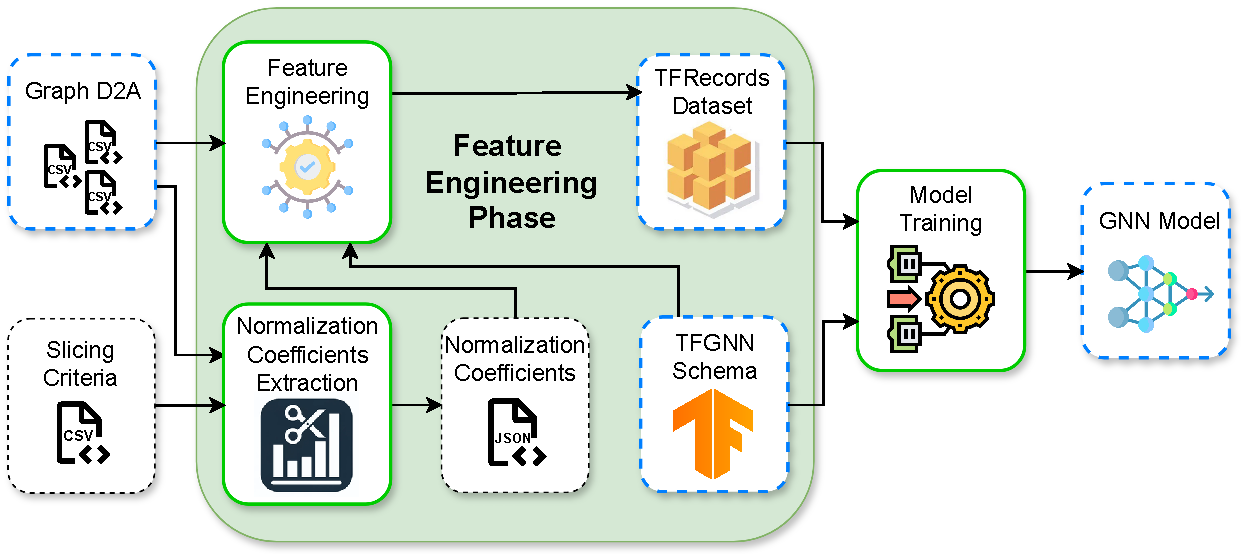
\includegraphics[width=0.95\textwidth]{figures/feature-engineering-phase.pdf}
	\caption{The figure shows a schematic of the feature engineering phase -- the final phase of the training pipeline. Dashed boxes represent the intermediate products and generated data. A~blue outline highlights the important outputs of the pipeline, and a green outline indicates the tools developed in this thesis. Icons were taken from~\cite{icon-feature, icon-tfrecords, icon-model-training, icon-model}.}
	\label{figure:feature-enginering}
\end{figure}

In feature engineering, the aim is to refine raw ECPGs to a state where models can be as small as possible while learning and generalizing effectively. The ultimate goal in reducing false positives is to train models that work for \textit{cross-analysis} -- training on one project while performing \textit{inference} on a different, unseen project. None of the models compared in this thesis, specifically those from~\cite{D2A-zheng2021d2a, pujar2024analyzing}, function within cross-analysis. Thus, in feature engineering, adjustments will be made that should help achieve cross-analysis for GNNs. The aim is to remove information from raw ECPGs that could lead the GNN model to \textit{overfit} to individual samples or entire projects. These adjustments include, for instance, removing specific variable names or suppressing the original programming style (already managed by converting to LLVM IR). These modifications are described in detail later in this section.


\subsubsection{Feature Selection}
Feature selection is one of the most crucial parts of the training pipeline because it allows for the greatest reduction in graph sizes. Simultaneously, incorrect feature selection prevents the GNN models from efficiently extracting distinguishing patterns. This significant importance was the primary motivation for Graph D2A (raw EPCGs) to also be one of the outputs of this thesis. If feature selection was poorly executed, the resulting dataset would be unusable, providing only incomplete data for the task. Thanks to Graph D2A, experimenting with different feature selections in the future is possible.

It is important to choose node/edge sets and their attributes that best and most accurately describe the code from the perspective of potential errors. These optimized graphs should contain only the information needed to distinguish between true positives and false positives. Additionally, the aim is for models to generalize well to unseen projects; for instance, the model should not remember variable names and thus recognize specific projects/samples based on them. This section describes which node/edge sets and their attributes were chosen and why (also why some were not chosen). The following description includes only edge/node sets that were generated for LLVM IR (at least for a single sample). Node sets that did not occur (even if some additional information from their layer did, see Section~\ref{graph-d2a}) are \texttt{TYPE\_ARGUMENT}, \texttt{TYPE\_PARAMETER}, \texttt{CONTROL\_STRUCTURE}, \texttt{JUMP\_LABEL}, \texttt{JUMP\_TARGET}, \texttt{MODIFIER}, and \texttt{TYPE\_REF}. Template node sets (see Figure~\ref{figure:node-set-hierarchy}) are also not generated. The edges \texttt{RECEIVER}, \texttt{CONDITION}, \texttt{INHERITS\_FROM}, and \texttt{BINDS\_TO} are also not present in Graph D2A. Attributes not mentioned for a given node set, and that the node set does have (see Table~\ref{tab:attributes1}), contain only a single (or, for instance, two but useless) value across the entire dataset and thus do not provide any useful information. The following descriptions are based on the Joern documentation~\cite{joern-cpg-doc} and the examination of Graph D2A samples.

\paragraph{The \texttt{META\_DATA} Node Set}
The node set \texttt{META\_DATA} will not be used at all because all its attributes contain only a single value for all samples. The only exception might be \texttt{LANGUAGE}, which holds information about the language from which the ECPG was generated. This is useful when the system has multiple input languages, which theoretically could be true for the proposed system (thanks to converting the input language to LLVM IR). However, since each input language would first be compiled to LLVM IR, \texttt{LANGUAGE} would always have the value \texttt{'LLVM'}.

\paragraph{The \texttt{FILE} Node Set}
The node set \texttt{FILE} also contains only attributes with the same values across samples. The reason it does not contain information about files is LLVM Link -- the input file to Joern with LLVM bitcode is always just one, so the node set \texttt{FILE} contains only a single node. Thus, the node set will be completely removed. Simultaneously, the edge set \texttt{SOURCE\_FILE} will also be removed because it depends on the \texttt{FILE} node set.

\paragraph{The \texttt{NAMESPACE} Node Set}
The node set \texttt{NAMESPACE} will also be completely removed. LLVM IR does not have namespaces like other high-level languages. At best, the concept of namespaces can be discussed in relation to individual files. However, the same problem arises as with the \texttt{FILE} node set -- all code is in a single file and thus in a single namespace. The attribute \texttt{NAME} contains only the values \texttt{<global>} and \texttt{llvm-link\_global}. Analogously for the node set \texttt{NAMESPACE\_BLOCK}.

\paragraph{The \texttt{METHOD} Node Set}
The node set \texttt{METHOD} will be used, specifically its attributes:
\begin{itemize}
    \item \texttt{IS\_EXTERNAL} -- has values \texttt{true} and \texttt{false}, indicating whether the function's code is available (and therefore a ECPG) or not (dynamic library call).
    \item \texttt{ORDER} -- the value is always \texttt{0}, but it is retained for later node set merging (see below in this section).
    \item \texttt{FULL\_NAME} -- the full name of the function (e.g., \texttt{malloc}). Ideally, this information should be removed to prevent the model from remembering functions from individual D2A projects, reducing the likelihood of successful cross-analysis. However, it is necessary to distinguish functions for which no code is available. Functions from standard libraries are crucial to remember because, for instance, \texttt{malloc} or \texttt{free} are essential for detecting memory leak errors. Using \texttt{FULL\_NAME} only for \texttt{IS\_EXTERNAL} functions is logical because they often belong to standard libraries, avoiding project-specific function names. However, project-specific functions can also be dynamically linked, and standard functions can be linked statically. For now, \texttt{FULL\_NAME} will be used for all functions, and the usage limited to some functions only is left for future work.
\end{itemize}

The following attributes contain some information but will not be used:
\begin{itemize}
    \item \texttt{AST\_PARENT\_FULL\_NAME} -- for \texttt{METHOD} nodes, this is the name of the \texttt{NAMESPACE\_BLOCK}, which does not contain any useful information, as mentioned before.
    \item \texttt{FILENAME} -- analogously to \texttt{AST\_PARENT\_FULL\_NAME}.
    \item \texttt{LINE\_NUMBER} -- information about which line the definition is on (may be empty), this information is not crucial for error detection.
    \item \texttt{NAME} -- for \texttt{METHOD} nodes, it contains, like \texttt{FULL\_NAME}, the function name.
    \item \texttt{SIGNATURE} -- contains the function signature, which is potentially useful information. However, since the data types of individual nodes will be included later (including the arguments and return values of all functions) as separate nodes, the signature will be implicitly present in the graph structure, and the \texttt{SIGNATURE} attribute would be redundant.
\end{itemize}

\paragraph{The \texttt{METHOD\_PARAMETER\_IN} Node Set}
For the node set \texttt{METHOD\_PARAMETER\_IN}, only the \texttt{ORDER} attribute will be used (the order among siblings in the AST), which indicates the index/order of the parameter within the function declaration. The other attributes will not be used, namely:
\begin{itemize}
    \item \texttt{CODE} -- contains the parameter name, which is better removed to improve generalization between projects.
    \item \texttt{INDEX} -- always has the same value as \texttt{ORDER} and expresses the same information, so it is unnecessary redundancy.
    \item \texttt{NAME} -- contains the same value as \texttt{CODE} --  will be removed.
    \item \texttt{TYPE\_FULL\_NAME} -- information about the data type, but since data types will be modeled as separate nodes, this information is redundant.
    \item \texttt{IS\_VARIADIC} -- information on whether the parameter is variadic (denoted as \texttt{'...'} in C, e.g., in the \texttt{printf} function). This information will be discarded for future node set merging purposes, but it is still useful information.
\end{itemize}

\paragraph{The \texttt{METHOD\_PARAMETER\_OUT} Node Set}
Node set \texttt{METHOD\_PARAMETER\_OUT} will be completely removed because, for statically typed languages (like LLVM IR), it contains the same information as \texttt{METHOD\_PARAMETER\_IN} and would unnecessarily add redundant data. The edge set \texttt{PARAMETER\_LINK} is also removed because it connects \texttt{METHOD\_PARAMETER\_IN} and \texttt{METHOD\_PARAMETER\_OUT}.

\paragraph{The \texttt{METHOD\_RETURN} Node Set}
In the \texttt{METHOD\_RETURN} node set, only the \texttt{ORDER} attribute will be used, mainly due to the later merging of node sets. The attributes \texttt{CODE}, \texttt{DYNAMIC\_TYPE\_HINT\_FULL\_NAME} (which can be empty), and \texttt{TYPE\_FULL\_NAME} typically contain the same information about the data type, which will be discarded for the aforementioned reasons.

\paragraph{The \texttt{MEMBER} Node Set}
For the \texttt{MEMBER} node set, only the \texttt{ORDER} attribute will be used, indicating the order within the defined structure. Other attributes will not be used:
\begin{itemize}
    \item \texttt{CODE} -- contains the name of the component. The name of the component is not important for distinguishing true positives and false positives; only its type and order matter.
    \item \texttt{NAME} -- contains the same information as \texttt{CODE}.
    \item \texttt{TYPE\_FULL\_NAME} -- types will later be expressed via nodes.
\end{itemize}

\paragraph{The \texttt{TYPE} Node Set}
The \texttt{TYPE} node set contains the attributes \texttt{FULL\_NAME}, \texttt{NAME}, and \texttt{TYPE\_DECL\_FULL\_NAME}, which contain the same information -- the full name of the data type. Therefore, only \texttt{FULL\_NAME} will be retained (although any of them could be used). Based on the name, the data type can be distinguished into multiple categories, such as integer, float, pointer, function signature, etc. More information can be found below in this section. Modeling data types using external nodes greatly simplifies other nodes that (where appropriate) carry their own type information in their attributes, which can then be removed. Overall, graphs will be smaller (in terms of data quantity in attributes) and simpler.

\paragraph{The \texttt{TYPE\_DECL} Node Set}
The \texttt{TYPE\_DECL} node set does not add any new information for LLVM IR compared to the \texttt{TYPE} node set. The node set could be useful for languages with parameterizable types or classes like C++ or Java. Therefore, this node set is completely removed. However, it must be removed carefully because it connects important parts of the graphs -- \texttt{TYPE} nodes of structured types with their \texttt{MEMBER} nodes. More information on this is provided later in this section.

\paragraph{The \texttt{BLOCK} Node Set}
The \texttt{BLOCK} node set does not contain any useful information in its attributes. Its usefulness lies in how it connects other nodes in the AST. For instance, each function has its own \texttt{BLOCK} node that contains all top-level statements. \texttt{BLOCK} nodes are useful, for example, for determining variable scope and also as \textit{latent nodes}\footnote{\textbf{Latent node} -- a node in the graph that does not contain any information itself and serves purely as a connection between other nodes.} for passing information within GNN~\cite{tfgnn-data-prep}. Again, for future node set merging, the \texttt{ORDER} attribute is retained, as well as the \texttt{ARGUMENT\_INDEX} attribute. However, neither carries any useful information.

\paragraph{The \texttt{CALL} Node Set}
In the \texttt{CALL} node set, only the attributes \texttt{ORDER} and \texttt{ARGUMENT\_INDEX} will be retained. If the parent of the \texttt{CALL} node is another \texttt{CALL} node, then \texttt{ARGUMENT\_INDEX} indicates the position among the function call arguments. If the parent is a \texttt{BLOCK} node, \texttt{ARGUMENT\_INDEX} indicates the position among the commands contained in that \texttt{BLOCK} node. However, this information is not particularly important and will be removed later, but detection of this case can only be done by examining the graph, as described later in this section.

\paragraph{The \texttt{FIELD\_IDENTIFIER} Node Set}
LLVM IR supports the array data type~\cite{LLVM-IR}, so the \texttt{FIELD\_IDENTIFIER} node set must be included. Again, the \texttt{ORDER} and \texttt{ARGUMENT\_INDEX} attributes are retained due to the later merging of node sets, although they contain the same value across the dataset. Both values are always \texttt{2}, because access to an array is modeled in ECPGs as a call to the \texttt{getElementPtr} operator, where the \texttt{FIELD\_IDENTIFIER} is always the second argument. The \texttt{CANONICAL\_NAME} attribute, which contains the name of the field, will not be included for reasons similar to those for the \texttt{FULL\_NAME} attribute in the \texttt{METHOD} node set -- the model should not remember samples/projects based on specific names.

\paragraph{The \texttt{IDENTIFIER} Node Set}
In the \texttt{IDENTIFIER} node set, only \texttt{ARGUMENT\_INDEX} and \texttt{ORDER} are retained, which now contain valid values. Other attributes are not included:
\begin{itemize}
    \item \texttt{CODE} -- contains the name of the variable, which is not used for the same reasons as \texttt{CANONICAL\_NAME} in \texttt{FIELD\_IDENTIFIER}.
    \item \texttt{COLUMN\_NUMBER} -- potentially useful information, especially for refining pooling in the GNN head (see Section~\ref{gnn-model}), but this is left for future improvements.
    \item \texttt{LINE\_NUMBER} -- same reason as \texttt{COLUMN\_NUMBER}.
    \item \texttt{NAME} -- contains the same information as \texttt{CODE}.
    \item \texttt{TYPE\_FULL\_NAME} -- types are handled using the \texttt{TYPE} node set.
\end{itemize}
This may raise the question of how to identify \texttt{IDENTIFIER} nodes that refer to the same variable in the graph when their names are discarded. The answer lies in the \texttt{LOCAL} nodes and \texttt{REF} edges that connect nodes representing the same variable. This information is thus represented by the graph structure and not by the node attributes.

\paragraph{The \texttt{LITERAL} Node Set}
In the \texttt{LITERAL} node set, the \texttt{ORDER} and \texttt{ARGUMENT\_INDEX} attributes are retained. Additionally, the \texttt{CODE} attribute, which contains the literal value, is also retained. This value can be an integer, floating point, string, array, structure, or any supported data type in LLVM IR~\cite{LLVM-IR}. Storing this value will require the creation of a~special node set capable of accommodating these different formats (see later in this section). The \texttt{COLUMN\_NUMBER}, \texttt{LINE\_NUMBER}, and \texttt{TYPE\_FULL\_NAME} attributes are not used for the reasons mentioned earlier.

\paragraph{The \texttt{LOCAL} Node Set}
In the \texttt{LOCAL} node set, only the \texttt{ORDER} attribute is used. Other attributes, such as \texttt{CODE}, \texttt{NAME}, and \texttt{TYPE\_FULL\_NAME}, are not used for the previously mentioned reasons. The usefulness of this node set lies mainly in connecting the \texttt{IDENTIFIER} nodes that represent the same variable. The problem is that \texttt{LOCAL} nodes only exist for local variables, not for global ones. LLVM IR can have global variables, but unfortunately, LLVM2CPG and Joern cannot properly encode them in the graph. Consider the read and write operations in Listing~\ref{listing:llvm-global-var}. It is clear which variable is being read/written to -- the \texttt{x}~and \texttt{y} variables. However, if ECPG is generated using LLVM2CPG and Joern, each access to a global variable is preceded by obtaining its address, and then the data is written/read to/from that address -- the variable identifier is not used. Obtaining the address is modeled as a call (a \texttt{CALL} node) to the \texttt{addressOf} operator, which has a single operand that should contain the global variable identifier in this case. But as shown in Listing~\ref{listing:ecpg-global-var}, the operand is of type \texttt{LITERAL} with value \texttt{0} and type \texttt{i32}. Therefore, global variables cannot be distinguished from each other. One possible way would be to use the debug info \texttt{!dbg !40} in the original LLVM IR (see Listing~\ref{listing:llvm-global-var}), which points to the exact location (line and column) in the original C code, and thus the name of the global variable could be extracted from there. However, this encounters the previously mentioned problem -- variables versus macros. Extracting global variables is thus left for future improvements.


\begin{lstlisting}[
    language=none, 
    label={listing:llvm-global-var}, 
    float=t,
    caption={An example of a code in LLVM IR that demonstrates reading and writing to global variables.}
]
 store i32 %5, i32* @x, align 4, !dbg !40    // write x
 %10 = load i32, i32* @x, align 4, !dbg !27  // load x
 store i32 %6, i32* @y, align 4, !dbg !42    // write y
 %7 = load i32, i32* @y, align 4, !dbg !24   // load y 
\end{lstlisting}

\begin{lstlisting}[
    language=none, 
    label={listing:ecpg-global-var}, 
    float=t,
    caption={The simplified ECPG in the CSV format for the LLVM IR code from Listing~\ref{listing:llvm-global-var}, demonstrating reading and writing to global variables.}
]
 // node set CALL
 ID,LABEL,CODE,COLUMN_NUMBER,LINE_NUMBER,METHOD_FULL_NAME,TYPE_FULL_NAME
 35,CALL,&0,16,10,<operator>.addressOf,i32*
 46,CALL,&0,16,12,<operator>.addressOf,i32*
 88,CALL,&0,5,7,<operator>.addressOf,i32*
 96,CALL,&0,5,8,<operator>.addressOf,i32*
 
 // edge set AST
 START_ID,END_ID,TYPE
 35,34,AST
 46,45,AST
 88,87,AST
 96,95,AST
 
 // node set LITERAL
 ID,LABEL,CODE,COLUMN_NUMBER,LINE_NUMBER,TYPE_FULL_NAME
 34,LITERAL,0,16,10,i32
 45,LITERAL,0,16,12,i32
 87,LITERAL,0,5,7,i32
 95,LITERAL,0,5,8,i32
\end{lstlisting}

\paragraph{The \texttt{METHOD\_REF} Node Set}
In the \texttt{METHOD\_REF} node set, only \texttt{ARGUMENT\_INDEX} and \texttt{ORDER} will be retained. The \texttt{COLUMN\_NUMBER} and \texttt{LINE\_NUMBER} attributes will not be retained for the reasons mentioned earlier. The \texttt{CODE} and \texttt{METHOD\_FULL\_NAME} attributes both contain the name of the method that the node represents. However, since \texttt{METHOD\_REF} is connected to the \texttt{METHOD} node via \texttt{REF} edges, these attributes can be discarded.

\paragraph{The \texttt{RETURN} Node Set}
In the \texttt{RETURN} node set, \texttt{ORDER} and \texttt{ARGUMENT\_INDEX} are used, which contain useful values. The location information \texttt{COLUMN\_NUMBER} and \texttt{LINE\_NUMBER} are discarded again.

\paragraph{The \texttt{UNKNOWN} Node Set}
In the \texttt{UNKNOWN} node set, only \texttt{ORDER} and \texttt{ARGUMENT\_INDEX} will be retained, both containing valid values. The \texttt{CODE} attribute may contain clues about what the \texttt{UNKNOWN} node holds -- typically the name of a data type or a signature. The \texttt{UNKNOWN} node itself does not provide any useful information, but it is typically deeply embedded in the graph and connects surrounding nodes. Because there are significantly fewer \texttt{UNKNOWN} nodes compared to other nodes, it will be retained.

\paragraph{Edge Sets}
The edge set \texttt{ALIAS\_OF} is discarded because aliases are resolved and the original type names are used during compilation and generating LLVM bitcode. Information about aliases is present in the graph through debugging information (see Section~\ref{bitcode-generation}) in the form of \texttt{TYPE} nodes. However, these nodes are later removed as part of graph optimizations (see below in this section).

The edge sets \texttt{AST}, \texttt{CFG}, and \texttt{CDG} are, of course, retained because they form the core of the CPG.

The edge set \texttt{ARGUMENT} is retained because it connects \texttt{CALL} nodes to their arguments.

The \texttt{CALL} edge set connects \texttt{CALL} nodes to their corresponding \texttt{METHOD} nodes, thereby adding a call graph to the CPG. The AST itself is created for each function, but the trees are not interconnected, preventing message propagation during GNN computation. The \texttt{CFG} edges, along with \texttt{CALL} edges, connect these individual ASTs at semantically appropriate places.

The edge sets \texttt{DOMINATE} and \texttt{POST\_DOMINATE} form dominator and post-dominator trees~\cite{princeton-dominators}, which provide useful information but essentially express certain simple properties of the CFG more explicitly. Additionally, there are too many of these edges, so they will not be used. However, it would be beneficial to experiment with them in future work.

The \texttt{REACHING\_DEF} edge set will not be used because there are too many of these edges in each graph. However, this is another very useful edge set that is worth experimenting with in future work.

The \texttt{CONTAINS} edge set will not be used because it also represents a relatively large number of additional edges. Furthermore, the information about which method a node belongs to can easily be obtained from the AST.

The \texttt{EVAL\_TYPE} edge set is, of course, used to connect nodes with their types.

The \texttt{REF} edge set is also retained to link identifiers to the local variable they identify. It also connects \texttt{METHOD\_REF} nodes and \texttt{METHOD} nodes.

\paragraph{Mandatory Attributes}
All node sets also contain the \texttt{ID} and \texttt{LABEL} attributes, which are not mentioned in the documentation. There are more undocumented attributes, such as \texttt{CLOSURE\_BINDING\_ID} in the \texttt{LOCAL} node set. However, since none of them are used, they are not mentioned in the text. A~complete list of attributes for node sets in Graph D2A can be found in Table~\ref{tab:attributes1}. The \texttt{ID} attribute identifies a node within each Graph D2A sample, and the \texttt{LABEL} attribute contains the name of the node set. Both of these attributes are used, although the \texttt{ID} is more for implementation reasons, and the original \texttt{ID} is not present in the output TFRecords files, which instead use IDs from the TFGNN library (see Section~\ref{implementation-feature-engineering}). Each edge set (except \texttt{REACHING\_DEF}, which contains an additional attribute) contains the following three attributes:
\begin{itemize}
    \item \texttt{START\_ID} -- the source node of the directed edge.
    \item \texttt{END\_ID} -- the target node of the directed edge.
    \item \texttt{TYPE} -- the name of the edge set.
\end{itemize}


\paragraph{Control Structures in Raw ECPGs}
The generated ECPGs do not contain the node sets \texttt{CONTROL\_STRUCTURE}, \texttt{JUMP\_LABEL}, or \texttt{JUMP\_TARGET}, even though the original C source code uses them. The reason lies partly in the conversion to LLVM IR and partly in generating the CPGs. During the compilation to LLVM IR, all control structures (\texttt{if}, \texttt{for}, \texttt{while}, etc.) are simplified to jumps. Consider a~simple \texttt{if} statement in C in Listing~\ref{listing:if-c}. The same code in LLVM IR is shown in Listing~\ref{listing:if-llvm}, where label \texttt{6:} represents the true branch and label \texttt{7:} the false branch of the original code. The tools LLVM2CPG and Joern did not generate \texttt{JUMP\_LABEL} or \texttt{JUMP\_TARGET} even though they are present. However, program branching information (which is crucial) can still be extracted from the CPG, specifically using \texttt{CFG} and \texttt{CDG} edges.

Consider a partial ECPG (only \texttt{CFG} and \texttt{CDG} edges and without the \texttt{ret} statement) in Figure~\ref{figure:if}, representing the LLVM IR code from Listing~\ref{listing:if-llvm}. If a node branches \texttt{CFG} edges (node \texttt{30}, representing the value assignment to \texttt{\%5}), the program flow branches at that node. The possible \texttt{CFG} paths are branches in the original code. These branches are connected to the condition that determines the program flow branching via \texttt{CDG} edges (from node \texttt{30}). 

From the graph, one can distinguish the true branch (assigning \texttt{1} to \texttt{\%1}) from the false branch (assigning \texttt{2} to \texttt{\%1}) because the true branch has \textbf{lower} \texttt{ORDER} value for the last node (node \texttt{34}) before the paths merge (node \texttt{40}) than the node from the false branch (node \texttt{38}). This is because the true branch is always first due to the compilation. If the LLVM IR is manually modified and the branches are rearranged, it will no longer be possible to distinguish the true and false branches from the graph. This fact further demonstrates that utilizing node sets and edge sets constructing the CPG is necessary. It also shows the importance of \texttt{ORDER} attributes in AST nodes.



\begin{lstlisting}[
    language=none, 
    label={listing:if-c}, 
    float=t,
    caption={A simple \texttt{if} statement in the C language.}
]
 if (z)
     return 1;
 else
     return 2;
\end{lstlisting}

\begin{lstlisting}[
    language=none, 
    label={listing:if-llvm}, 
    float=t,
    caption={The code from Listing~\ref{listing:if-c}, but converted to LLVM IR.}
]
   %5 = icmp ne i32 %4, 0, !dbg !16
   br i1 %5, label %6, label %7, !dbg !18

 6:
   store i32 1, i32* %1, align 4, !dbg !19
   br label %8, !dbg !19

 7:
   store i32 2, i32* %1, align 4, !dbg !20
   br label %8, !dbg !20

 8:
   %9 = load i32, i32* %1, align 4, !dbg !21
   ret i32 %9, !dbg !21
\end{lstlisting}

\begin{figure}[t]
	\centering
	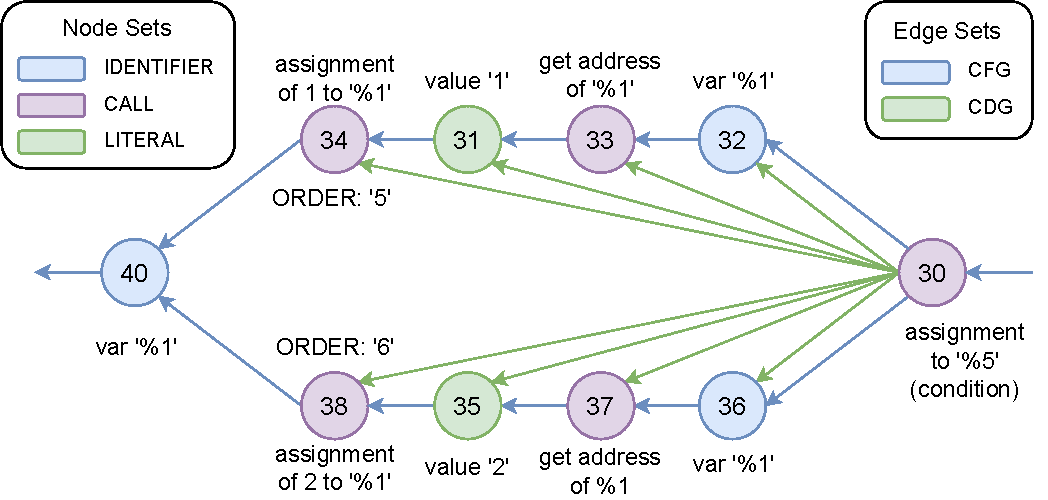
\includegraphics[width=1\textwidth]{figures/ecpg-if.pdf}
	\caption{A~partial (only \texttt{CFG} and \texttt{CDG} edges and without the \texttt{ret} statement) ECPG demonstrating branching in LLVM IR from Listing~\ref{listing:if-llvm}.}
	\label{figure:if}
\end{figure}
    
The node sets and their attributes present in Graph D2A are listed in Table~\ref{tab:attributes1}. Attributes of individual node sets that were considered useful and selected during feature selection are also marked in the table.

\subsubsection{Graph Structure Optimization}
Before using individual graphs as inputs to GNNs, it is necessary to remove as many unnecessary and redundant nodes, edges, and attributes from the graphs as possible. The previous text dealt with the removal of information at the level of entire node sets, edge sets, and attributes. However, even within a single node set, there are nodes that do not add any useful information and can be removed, effectively reducing the graph and easing the learning process of the GNNs. Furthermore, adjustments are required to ensure certain properties arising from the use of GNNs and the TFGNN library.

To propagate information correctly within the graph during GNN computation, the graph must consist of only one WCC (see Section~\ref{gnn}). For GNNs where message passing follows the direction of the edges, it is also necessary to ensure the correct orientation of the edges. Using TFGNN requires creating a so-called TFGNN schema~\cite{tfgnn-schema}, which describes the graph structure: node sets, edge sets, their attributes, and attribute data types. In the TFGNN schema, all nodes in a node set must have the same attributes (similarly for edges) -- this already applies to raw ECPGs. Furthermore, each edge set must have a fixed source node set and target node set -- unfortunately, this is not the case with raw ECPGs. For example, \texttt{AST} edges connect \texttt{BLOCK}, \texttt{CALL}, \texttt{LOCAL}, \texttt{IDENTIFIER}, and other types of nodes.

The following transformations are described in this section:
\begin{enumerate}
    \item removal of unnecessary and redundant information,
    \item creating graphs with only one WCC,
    \item ensuring fixed source and target node sets for all edge sets.
\end{enumerate}

The removal of unnecessary and redundant information and ensuring a single WCC are closely related because removing some unnecessary nodes also removes unnecessary separate WCCs. This step consists of the following sub-steps, which must be performed in the given order:
\begin{enumerate}
    \item removal of invalid nodes within the AST,
    \item removal of WCCs (only in the AST) consisting only of \texttt{BLOCK} nodes,
    \item removal of AST leaf \texttt{BLOCK} nodes,
    \item filtering out unnecessary \texttt{ARGUMENT} edges,
    \item removal of AST children of external functions,
    \item removal of unused functions,
    \item filtering out unnecessary \texttt{EVAL\_TYPE} edges,
    \item removal of the \texttt{TYPE\_DECL} node set,
    \item filtering out unused \texttt{TYPE} nodes.
\end{enumerate}

\paragraph{Removal of Invalid Nodes}
The removal of invalid nodes occurs only within the AST -- considering only \texttt{AST} edges and ignoring others. Invalid nodes are considered all those that were removed during feature selection and have an \texttt{AST} edge leading to or from them (e.g., a standalone \texttt{META\_DATA} node is not part of the AST). If these nodes were simply removed (along with their edges), the AST they belong to would be split. Therefore, they need to be removed based on their position in the AST as follows:
\begin{enumerate}
    \item Leaf -- the invalid node, along with its edges, can be simply removed.
    \item Root -- the invalid node is replaced with a valid \texttt{BLOCK} node to ensure that the AST has exactly one valid root.
    \item Inner node -- the AST children of the invalid node are connected to the AST parent of the invalid node.
\end{enumerate}

Since no node types inheriting from \texttt{CFG\_NODE} are removed during feature selection, it is not necessary to connect \texttt{CFG} edges in the case of inner nodes because there should not be any, according to the documentation. Similarly, \texttt{CDG} edges do not make sense for any invalid nodes. An exception is the removed \texttt{METHOD\_PARAMETER\_OUT} node set, which inherits from \texttt{CFG\_NODE} (see Figure~\ref{figure:node-set-hierarchy}), but no \texttt{CFG} or \texttt{PDG} edges leading to or from these nodes were found in Graph D2A. Therefore, only \texttt{AST} edges need to be reconnected. 

After removing the invalid nodes, the graph is composed of one or more ASTs -- one AST for each function.

\paragraph{Removal of \texttt{BLOCK} WCCs}
After removing the invalid nodes, it is necessary to remove WCCs entirely composed of \texttt{BLOCK} nodes. These are latent nodes, and WCCs entirely composed of latent nodes contain no useful information. Such WCCs can arise, for example, from ASTs entirely composed of invalid nodes, as the previous algorithm would convert the invalid root into a valid node and remove the other invalid nodes. This would result in an AST with only a \texttt{BLOCK} node. The case where a WCC consists only of \texttt{BLOCK} nodes is relatively rare.

\paragraph{Removal of Leaf \texttt{BLOCK} Nodes}
All leaf \texttt{BLOCK} nodes are also removed from all ASTs. The reason is that \texttt{BLOCK} nodes are used to cluster other nodes -- if they have no AST children, they are unnecessary.

\paragraph{Filtering of \texttt{ARGUMENT} Edges}
Next, the \texttt{ARGUMENT} edge set is filtered to keep only edges that have a \texttt{CALL} node as their source. In other words, the \texttt{ARGUMENT} edges between \texttt{RETURN} nodes and the expressions they return (nodes inheriting from \texttt{EXPRESSION}) will be removed. This adjustment is made to move the \texttt{ARGUMENT\_INDEX} into the \texttt{ARGUMENT} edges later. For \texttt{ARGUMENT} edges from \texttt{RETURN} nodes, it does not make sense to talk about the index of arguments (there is always only one for LLVM IR~\cite{LLVM-IR}), so these edges are removed.

\paragraph{Removal of \texttt{AST} Children of External Functions}
All AST children of \texttt{METHOD} nodes representing external functions (having the value \texttt{True} in the \texttt{IS\_EXTERNAL} attribute) are then removed. The removed nodes for each function are one \texttt{METHOD\_RETURN} and $N$ \texttt{METHOD\_PARAMETER\_IN}, where $N$ is the number of function parameters. For external functions, this information is not useful because the information about input and output parameters is already present when calling the function (\texttt{CALL} node and its AST children). \texttt{METHOD\_PARAMETER\_IN} serves only as a link between arguments from the call site and the use of parameters within the function body for non-external functions. Similarly, \texttt{METHOD\_RETURN} serves as an abstraction of all \texttt{RETURN} nodes (typically only a single \texttt{ret} statement in each function, see Listing~\ref{listing:if-llvm}) in the function body -- it is connected to them. 

Another reason for removing AST children of external functions is that for many operators, \texttt{EVAL\_TYPE} edges led from the \texttt{METHOD\_PARAMETER\_IN} and \texttt{METHOD\_RETURN} nodes to a \texttt{TYPE} node, whose type was \texttt{ANY} -- which does not provide any additional information. By removing these AST children, these \texttt{EVAL\_TYPE} edges are also removed, leading to the removal of the \texttt{TYPE} node with the \texttt{ANY} value. Thus, the data type \texttt{ANY} will not need to be considered.

\paragraph{Removal of Unused Functions}
If an unused function is found -- in other words, if there is a \texttt{METHOD} node in the graph without incoming \texttt{CALL} edges -- it is also removed. This can happen because each graph implicitly includes at least the function \texttt{llvm.dbg.declare}, which is part of the debug information~\cite{LLVM-IR}. There may also be some unused operators or other default global functions.

\paragraph{Filtering of \texttt{EVAL\_TYPE} Edges}
The next step is the removal of \texttt{EVAL\_TYPE} edges leading from the \texttt{METHOD}, \texttt{BLOCK}, and \texttt{METHOD\_REF} nodes. All these node sets contain information about the data type, which do not need to be retained. For \texttt{BLOCK} nodes, this represents the return type of the entire block -- in some languages (typically functional), this information is useful, but in C/LLVM IR, this value is irrelevant as it merely indicates the data type of the last statement in the given block. For \texttt{METHOD} and \texttt{METHOD\_REF}, it represents the signature, which (as previously mentioned) is expressed through the data types of the function's inputs and outputs.

\paragraph{Removal of the \texttt{TYPE\_DECL} Node Set}
In feature selection, it was mentioned that the \texttt{TYPE\_DECL} node set needs to be removed in a~specific way because it connects structures and their elements. If a \texttt{TYPE} node is a~structure for which its \texttt{MEMBER} nodes are known (if only a pointer to it is used, the elements may not be known), then this \texttt{TYPE} node is connected by a \texttt{REF} edge to a \texttt{TYPE\_DECL} node, from which \texttt{AST} edges lead to individual \texttt{MEMBER} nodes, as shown in Figure~\ref{figure:struct}. Each \texttt{TYPE\_DECL} is then removed such that if it has any AST \texttt{MEMBER} children, these \texttt{MEMBER} (target node) nodes are connected to the \texttt{TYPE} node (source node) using new \texttt{CONSISTS\_OF} edges, and the \texttt{TYPE\_DECL} is removed along with all edges leading to or from it. If the \texttt{TYPE\_DECL} has no \texttt{AST} \texttt{MEMBER} children, it can simply be removed.

\begin{figure}[t]
	\centering
	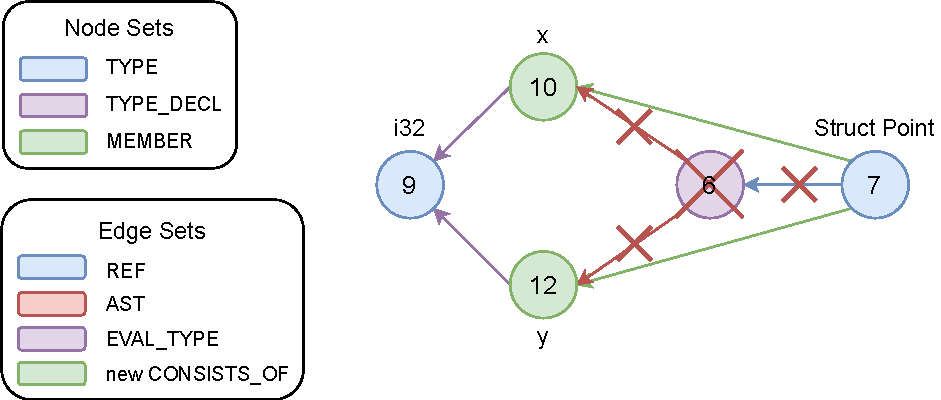
\includegraphics[width=0.85\textwidth]{figures/ecpg-struct.pdf}
	\caption{The figure shows the connection of \texttt{TYPE\_DECL} nodes in ECPG when modeling structured data types.}
	\label{figure:struct}
\end{figure}

\paragraph{Filtering of Unused \texttt{TYPE} Nodes}
Unused \texttt{TYPE} nodes are then removed. An unused \texttt{TYPE} node has no incoming \texttt{EVAL\_TYPE} edges. This removal process is iterative -- it iterates until there are no \texttt{TYPE} nodes without incoming edges. This ensures that nested or recursive structures are also removed. One might ask what happens if a \texttt{TYPE} node has a self-loop (loop) -- a recursive structure (or two or more mutually recursive structures). The answer lies in the representation of such structures -- a recursive structure cannot contain itself, only a pointer to itself (similarly for mutual recursion). Self-loops and loops are not possible for \texttt{TYPE} nodes because \texttt{MyStruct} and \texttt{MyStruct*} are two different types, represented by two \texttt{TYPE} nodes. For this reason, the information about the individual elements of \texttt{MyStruct} does not need to be present in the graph if only its pointer \texttt{MyStruct*} is used and its elements are not accessed -- information about the elements would be redundant.

As a result of these modifications, the graph is composed of a single WCC. When using bi-directional GNNs, information can be propagated between all nodes. For directional GNNs , it is still necessary to correctly orient the edge sets, as described below.

\paragraph{The Edge Set Condition}
The condition set by the TFGNN schema that each edge set must have a fixed source node set and target node set is currently not met. Examples include the basic \texttt{AST} edges that start and end in different node sets. This condition can be met in two basic ways:
\begin{enumerate}
    \item Splitting all edge sets that do not meet the conditions into smaller edge sets to meet the condition. The problem with this solution is that the number of possible sub edge sets is up to $|N|^2$ where $N$ is the set of node sets that can appear on either side of any edge in the given edge set -- because it is necessary to cover each combination of node sets. Of course, some combinations are not possible, such as a \texttt{METHOD} node not having direct AST children of the type \texttt{CALL}, so practically, there are fewer combinations. Adding the fact that even \texttt{CFG} and \texttt{PDG} also connect a large number of node sets, like \texttt{AST}, this number increases significantly. This results in dealing with tens to hundreds of sub edge sets. The fact that it would be necessary to define them manually in the TFGNN schema, and the fact that the more edge sets there are, the more complex the GNN model, shows that this number of sub edge sets is unsustainable. The principle is demonstrated in Figure~\ref{figure:tfgnn-condition}.
    \item Some existing node sets can be merged so that all edge sets meet the required condition. This method simplifies the TFGNN schema (there will be fewer node sets) but requires that all node sets that will be merged into a super node set have the same attributes. For this reason, potentially useful attributes were discarded and some unnecessary attributes were retained during the feature selection phase. The principle is also demonstrated in Figure~\ref{figure:tfgnn-condition}.
\end{enumerate}


\begin{figure}[t]
	\centering
	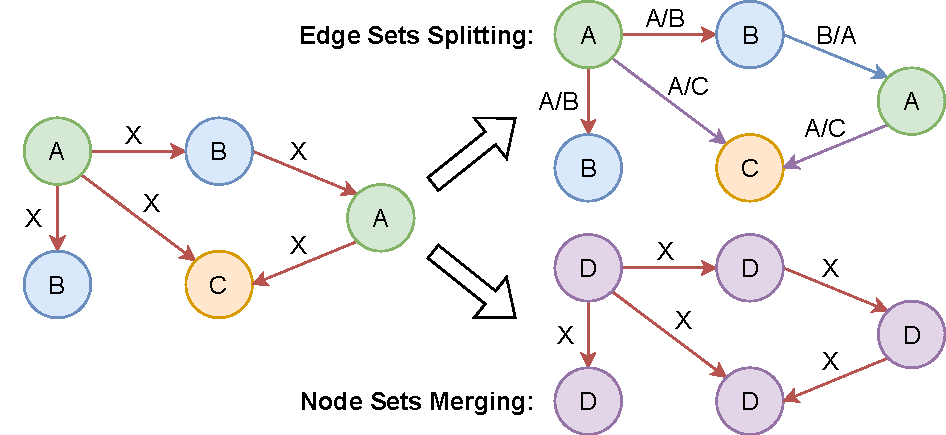
\includegraphics[width=0.8\textwidth]{figures/tfgnn-condition.pdf}
	\caption{The figure demonstrates two basic ways to meet one of the conditions set by the TFGNN schema -- that each edge set has exactly one source and target node set.}
	\label{figure:tfgnn-condition}
\end{figure}

\paragraph{Merging of Node Sets}
The condition is thus ensured in this thesis by merging certain node sets. Although efforts were made in the feature selection phase to ensure that all node sets to be merged in the future have the same attributes, some attributes are too important to discard. The problem of different attribute sets when merging node sets can be solved in two extreme approaches:
\begin{enumerate}
    \item \textit{Sparse nodes} -- create a set of all attributes contained in the merged node sets. The output super node set will have all these attributes. If an attribute does not make sense for a particular node, it is simply replaced with an invalid value. This principle is simple but creates sparse nodes and effectively increases the graph's data size. The principle of merging node sets using sparse nodes is demonstrated in Figure~\ref{figure:sparse-nodes}.
    
    \item Latent nodes -- the exact opposite approach is extracting each node's attributes into a special \textit{data node} connected to the original node by a special edge set, according to the original node set. This again effectively unifies the node format. This principle is somewhat more complex because it requires the creation of new edge sets connecting latent nodes with their data nodes. The number of these new edge sets is $|N|$, where $N$ is the set of merged original node sets. However, the output is a graph that is smaller in data size but larger in the number of nodes. Another advantage is that data nodes will (when using oriented GNNs) constantly send information about the original data, as their values will not be overwritten during GNN computation because they have no incoming edges. The principle of merging node sets using latent nodes is demonstrated in Figure~\ref{figure:latent-nodes}.
\end{enumerate}

\begin{figure}[t]
	\centering
	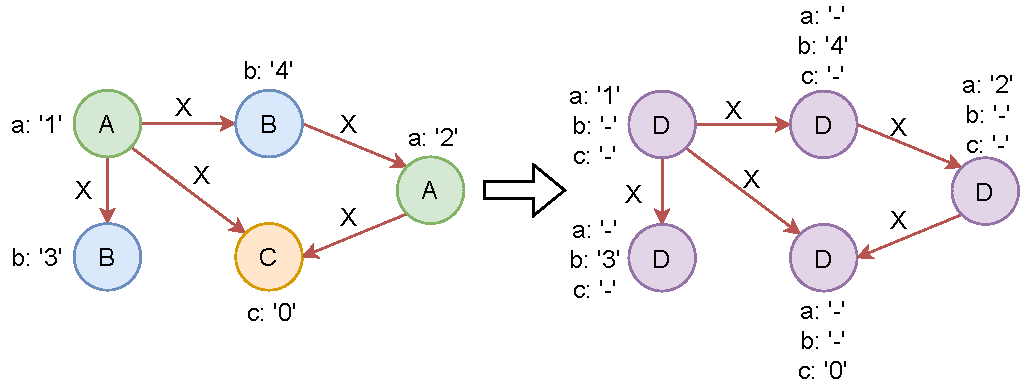
\includegraphics[width=0.93\textwidth]{figures/sparse-nodes.pdf}
	\caption{The figure demonstrates merging node sets using sparse nodes -- the super node set contains attributes of all original node sets. The original graph is from Figure~\ref{figure:tfgnn-condition} and is supplemented with node set attributes.}
	\label{figure:sparse-nodes}
\end{figure}

\begin{figure}[t]
	\centering
	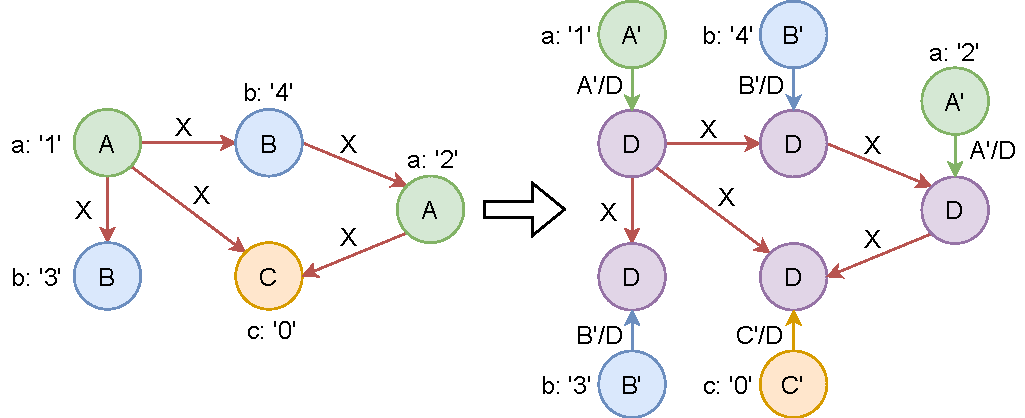
\includegraphics[width=0.93\textwidth]{figures/latent-nodes.pdf}
	\caption{The figure demonstrates merging node sets using latent nodes -- the attributes of the original node sets are extracted into special data node sets. The original graph is from Figure~\ref{figure:tfgnn-condition} and is supplemented with node set attributes.}
	\label{figure:latent-nodes}
\end{figure}

Both approaches have their advantages and disadvantages. In this work, the \textit{mixed nodes} approach is used -- a combination of the best properties of both approaches. For attributes that are common to all/most original node sets (e.g., \texttt{ORDER} for all nodes inheriting from \texttt{AST\_NODE}), the sparse node approach is used. On the other hand, for attributes that are specific to certain node sets (e.g., \texttt{CODE} for \texttt{LITERAL}, containing the literal value), the latent node approach is used. Here, however, the latent node is not empty but contains previously defined sparse attributes. By combining these methods, the graphs are small in both node count and attribute count, while only requiring the definition of a few new edge and node sets to connect data nodes with specific attributes. Table~\ref{tab:merged-node-sets} shows all selected node sets and attributes in the feature selection phase and their combination into new node sets.

\paragraph{The New \texttt{AST\_NODE} Node Set}
The new node set \texttt{AST\_NODE} consists of original node sets that are connected by \texttt{AST} edges. All these node sets inherit from the template node set \texttt{AST\_NODE} (hence the same name), see Figure~\ref{figure:node-set-hierarchy}. These original node sets thus represent the code as such -- the AST. Thanks to the new \texttt{AST\_NODE} set, it is possible to keep the \texttt{AST}, \texttt{CFG}, \texttt{CDG}, \texttt{REF}, and \texttt{ARGUMENT} edge sets intact -- their target and source node sets will be the new \texttt{AST\_NODE} node set. The \texttt{AST\_NODE} node set contains sparse attributes:
\begin{itemize}
    \item \texttt{LABEL} -- indicates the original node set (e.g., \texttt{BLOCK}, \texttt{LOCAL}, \texttt{METHOD}, etc.); each node contains it, so there is no need to fill it with invalid values.
    \item \texttt{ORDER} -- is also present in all nodes.
    \item \texttt{ARGUMENT\_INDEX} -- for the original node sets \texttt{METHOD}, \texttt{LOCAL}, \texttt{METHOD\_RETURN}, and \texttt{METHOD\_PARAMETER\_IN}, this information needs to be filled with zeros, see Table~\ref{tab:merged-node-sets}. However, \texttt{ARGUMENT\_INDEX} will be completely removed later, as explained below.
\end{itemize}

\paragraph{New Data Node Sets}
From Table~\ref{tab:attributes1}, it is evident that the original node sets \texttt{METHOD} and \texttt{LITERAL} contain special attributes that require the creation of data nodes. For the \texttt{METHOD} node set, the attributes \texttt{FULL\_NAME} and \texttt{IS\_EXTERNAL} need to be separated. The new data node set for the \texttt{METHOD} node set is named \texttt{METHOD\_INFO} and is connected using the \texttt{METHOD\_INFO\_LINK} edge set, where the source is \texttt{METHOD\_INFO} and the target is the new \texttt{AST\_NODE} node set (original \texttt{METHOD} nodes). Similarly, for \texttt{LITERAL}, the \texttt{CODE} attribute needs to be separated into the \texttt{LITERAL\_VALUE} node set and connected using the \texttt{LITERAL\_VALUE\_LINK} edge set, with the source being \texttt{LITERAL\_VALUE} and the target being the new \texttt{AST\_NODE} (original \texttt{LITERAL} nodes).

\paragraph{Retained Node Sets}
Node sets \texttt{MEMBER} and \texttt{TYPE} are retained. However, due to the creation of the new \texttt{AST\_NODE} from which \texttt{EVAL\_TYPE} edges originate, and the retention of \texttt{MEMBER} -- which also has \texttt{EVAL\_TYPE} edges -- it is necessary to split the \texttt{EVAL\_TYPE} edge set. The name \texttt{EVAL\_TYPE} is retained for edges originating from \texttt{AST\_NODE} and ending in \texttt{TYPE}. The new edge set \texttt{EVAL\_MEMBER\_TYPE} represents the remaining edges from \texttt{MEMBER} to \texttt{TYPE}. The reason why \texttt{MEMBER} and \texttt{TYPE} are kept in separate node sets is that they do not represent the code itself (description of computation) but provide additional information about types -- thus, the node sets are logically separated.

\paragraph{The New \texttt{ARGUMENT\_INDEX} Edge Attribute}
The penultimate adjustment is the transfer of the \texttt{ARGUMENT\_INDEX} attribute from the new node set \texttt{AST\_NODE} to the \texttt{ARGUMENT} edge set. However, this is not done for all nodes that have \texttt{ARGUMENT\_INDEX}, but only for those that are the target node for some \texttt{ARGUMENT} edge. At this stage, only \texttt{ARGUMENT} edges originating from the original \texttt{CALL} node set remain. The TFGNN schema allows attributes for both nodes and edges, and therefore, this transformation saves a considerable amount of data and reduces the complexity of the \texttt{AST\_NODE} nodes.

\paragraph{Orientation of Edges}
The final step is to correctly orient the edges in case oriented GNNs are used. The orientation of edge sets at this stage is shown in Table~\ref{tab:edge-sets-orientation}, where the edge sets that need to be reversed are highlighted in red. The reasons are:
\begin{itemize}
    \item \texttt{ARGUMENT} -- information about arguments will flow towards the \texttt{CALL} node, from which it will then propagate to the respective function.
    \item \texttt{EVAL\_TYPE} -- information about types will propagate to the nodes where it will be used -- it makes no sense to propagate information from \texttt{AST\_NODE} to be concentrated in \texttt{TYPE} nodes.
    \item \texttt{EVAL\_MEMBER\_TYPE} -- analogous to \texttt{EVAL\_TYPE}.
    \item \texttt{CONSISTS\_OF} -- information about individual \texttt{MEMBER} nodes will flow into the structure so that the structure node contains information about its members.
    \item \texttt{REF} -- here, information will propagate from \texttt{LOCAL} nodes to identifiers so that they know it is the same variable (different \texttt{LOCAL} nodes in the same function can be distinguished using the \texttt{ORDER} attribute). For \texttt{METHOD\_REF}, information about the given method will flow into that node -- the function is not called here, but it is desirable to attach information to it (reversed compared to \texttt{CALL} edges).
\end{itemize}

\begin{table}
    \centering
    \caption{The table contains source and target node sets for each used edge set (after feature selection). Edge sets highlighted in red have an incorrect orientation and will be reversed.}
    \vskip6pt
	\begin{tabular}{
        !{\vrule width 1pt}l!{\vrule width 1pt}l|l!{\vrule width 1pt}}
        \noalign{\hrule height 1pt}
        Edge Set & Source Node Set & Target Node Set \\
        \noalign{\hrule height 1pt}

        METHOD\_INFO\_LINK & METHOD\_INFO & AST\_NODE \\ \hline
        \rowcolor{lightred}
        EVAL\_MEMBER\_TYPE & TYPE & MEMBER \\ \hline
        \rowcolor{lightred}
        CONSISTS\_OF & MEMBER & TYPE \\ \hline
        AST & AST\_NODE & AST\_NODE \\ \hline
        LITERAL\_VALUE\_LINK & LITERAL\_VALUE & AST\_NODE \\ \hline
        \rowcolor{lightred}
        ARGUMENT & AST\_NODE & AST\_NODE \\ \hline
        CALL & AST\_NODE & AST\_NODE \\ \hline
        CFG & AST\_NODE & AST\_NODE \\ \hline
        CDG & AST\_NODE & AST\_NODE \\ \hline
        \rowcolor{lightred}
        EVAL\_TYPE & TYPE & AST\_NODE \\ \hline
        \rowcolor{lightred}
        REF & AST\_NODE & AST\_NODE \\ \hline
        
        \noalign{\hrule height 1pt}
    \end{tabular}
    \label{tab:edge-sets-orientation}
\end{table}

The orientation of the other edge sets is preserved for the following reasons:
\begin{itemize}
    \item \texttt{METHOD\_INFO\_LINK} and \texttt{LITERAL\_VALUE\_LINK} -- they originate from data nodes to latent nodes, allowing data information to spread further into the graph.
    \item \texttt{CFG} -- their direction reflects the program's control flow and the chronological order of node traversal, where the node order plays a crucial role in the manifestation of errors.
    \item \texttt{AST} -- reversing the edges would mean that it is no longer a tree, but this is not a~problem. From a message-passing perspective, the tree has an interesting property: information is copied down the tree -- parents send the same message to their children, and children have only a single parent. If the \texttt{AST} edges were reversed, information would flow to the original root node, and information from the children would need to be combined in some way (the term "\textit{pooling}" is used, see Section~\ref{gnn-model}), leading to an irreversible loss of information. However, it would be possible to read the final state from the root, where information from the entire graph would accumulate -- but the graph would have to be shallow enough for information to travel from all leaf nodes to the root (because, as mentioned in Section~\ref{gnn-model}, the number of message passes is a~hyperparameter of the model). Pooling still occurs in GNNs because nodes in ECPGs can have multiple incoming and outgoing edges. Thus, it might be interesting trying the reverse direction of the \texttt{AST} edges in the future.
    \item \texttt{CALL} -- similar reason as \texttt{CFG} -- it is a natural control flow of the code.
    \item \texttt{CDG} -- edges originate from nodes representing conditions to nodes affected by the condition. Thus, it is again in the correct chronological order.
\end{itemize}


\subsubsection{Atribute Transformation}
Another property that graphs must satisfy according to the TFGNN schema is that an attribute (from now on, referred to as a feature) has a fixed type~\cite{tfgnn-schema}. However, this is not yet the case; for example, the feature \texttt{CODE} in the \texttt{LITERAL} node can contain values of all data types in LLVM IR. Although all values can be considered strings in CSV, and TFGNN supports features of type \texttt{DT\_STRING}~\cite{tfgnn-schema}, it would be more challenging for the model to extract useful information from such complex features. To facilitate training, some complex features are decomposed into multiple simpler ones~\cite{feature-splitting}.

\paragraph{Features of the \texttt{AST\_NODE} Node Set}
The node set \texttt{AST\_NODE} has a feature \texttt{ORDER}, which is a simple integer type. The feature \texttt{LABEL} is also a simple type, with categorical values representing the names of the original node sets. To prevent the model from having to take a string as input, the feature label values are mapped to a simple integer type as follows: \texttt{UNKNOWN: 0}, \texttt{METHOD: 1}, ... ,\texttt{RETURN: 11}. The model does not need the \texttt{LABEL} feature in string format; it just needs to distinguish between different types, and the simplest representation is an integer.

\paragraph{Features of the \texttt{MEMBER} Node Set}
The node set \texttt{MEMBER} has only one feature, \texttt{ORDER}, which does not require any modification.

\paragraph{Features of the \texttt{METHOD\_INFO} Node Set}
The node set \texttt{METHOD\_INFO} contains the flag feature \texttt{IS\_EXTERNAL}, which contains values \texttt{True} and \texttt{False} since it is a flag. These boolean values are converted to integer values \texttt{1} and \texttt{0} for simplicity. The second feature is \texttt{FULL\_NAME}, which contains the name of the function. Since LLVM IR operators are modeled as functions in ECPGs, \texttt{FULL\_NAME} can include the prefix \texttt{<operator>.} followed by the operator's name, such as \texttt{notEquals}, \texttt{xor}, etc. Since operators are used much more frequently than functions and are also limited in number, it makes sense to convert them into their own categorical feature, \texttt{OPERATOR}. This feature contains the numerical designation of the operator if detected from the \texttt{FULL\_NAME} feature. If it is not an operator, the entire function name should be remembered. Here, there are several options for modeling the remaining values:
\begin{itemize}
    \item Keep the name as a string -- the model will need to contain, for example, some kind of RNN layer.
    \item Use word2vec~\cite{mikolov2013efficient} or a similar model that can encode a word into a vector while preserving its meaning.
    \item Use trainable embedded tables~\cite{tfgnn-gnn-modeling}.
    \item Hash the name.
\end{itemize}

In this work, the simplest and fastest approach, hashing, is used. The function name is hashed into 24 bits (the reason for 24 bits is explained below). This approach discards all information about the original name but allows the model to remember the occurrence of specific functions -- if a function frequently appears in the true positive class, it is likely associated with it and can serve as part of a learned pattern. Hashing was chosen because, compared to other methods, it is by far the fastest, and generating Graph D2A (and applying feature engineering) is already computationally expensive, as described in Chapter~\ref{implementation}. However, future work should include experiments with other string encoding methods.

\paragraph{Features of the \texttt{TYPE} Node Set}
For the node set \texttt{TYPE}, it is again necessary to decompose the feature \texttt{FULL\_NAME} into simpler features that can be better processed by the model. \texttt{FULL\_NAME} contains the name of the represented data type. LLVM IR supports a~number of data types~\cite{LLVM-IR} (here are the formats as they appear in the \texttt{FULL\_NAME} feature):
\begin{itemize}
    \item Pointer -- the suffix contains one or more \texttt{*} characters, e.g., \texttt{i32*}, \texttt{FILE*}, etc.
    \item Array -- the format is \texttt{[ LEN x TYPE ]}, e.g., \texttt{[114 x i8]}, \texttt{[114 x [114 x i8]]}, etc.
    \item Integer -- the format is \texttt{iN}, where \texttt{N} is an integer > 1 indicating the size of the type in bits, e.g., \texttt{i1} (boolean), \texttt{i32}, \texttt{i128}, etc.
    \item Floating point -- one of \texttt{half}, \texttt{float}, \texttt{double}, or \texttt{fp128}.
    \item Structs -- the format is \texttt{\{ TYPE1, TYPE2, ... \}}, e.g., \texttt{\{ i32, i32 \}}, \texttt{\{ i1, float, \{ i32, i32 \} \}}, etc.
    \item Function signature -- the format is \texttt{TYPE (TYPE1, ...)}, e.g., \texttt{i1 (i1, i8*)}, etc.
    \item Void -- represents an empty value, denoted as \texttt{void}.
    \item Named type -- everything else, e.g., \texttt{ngx\_radix\_tree\_t}, \texttt{FILE}, etc.
\end{itemize}

In the previous section, it was described that \texttt{TYPE} nodes with signatures were removed, so they do not need to be considered. Similarly, \texttt{TYPE} nodes with the value \texttt{ANY} were removed -- this is not an LLVM IR type but a value inserted by the Joern tool. The other data type names need to be appropriately represented using simpler data types. Thus, the feature \texttt{FULL\_NAME} is decomposed into the following primitive features:
\begin{itemize}
    \item \texttt{PTR} -- if the type is a pointer, this stores the pointer depth -- the number of trailing \texttt{*}~symbols.
    \item \texttt{LEN} -- if the type is an array, this stores its length (only the outer-most array is considered).
    \item \texttt{INT} -- if the type is an integer, this stores \texttt{N}, the number of bits.
    \item \texttt{FP} -- if the type is a floating point, this stores a categorical numerical designation of the given type.
    \item \texttt{HASH} -- if the type is a struct or a named type, this stores the 24-bit hash of its name. In the case of an array, it stores the 24-bit hash of the element type name (if it is not a primitive type, see below).
\end{itemize}

The individual features are set as follows and \textbf{in exactly this order}:
\begin{enumerate}
    \item All features are initialized to 0.
    \item \texttt{PTR} is set (it can also be 0), the trailing \texttt{*} are removed, and \textbf{processing continues}.
    \item \texttt{LEN} is set (it can also be 0), and if \texttt{LEN} > 0, the outer-most array is removed, leaving only the type of the elements, and \textbf{processing continues}.
    \item If the type is an integer, \texttt{INT} is set, and processing ends.
    \item If the type is a floating point or void, \texttt{FP} is set (0 in the case of void), and processing ends.
    \item The remaining type is an array, struct, or named type -- \texttt{HASH} is set (from the remaining name), and processing ends.
\end{enumerate}

From this, it follows that for the void type, all values are equal to 0, which semantically makes sense because it indicates the absence of a value.

\paragraph{Features of the \texttt{LITERAL\_VALUE} Node Set}
For the node set \texttt{LITERAL\_VALUE}, the feature \texttt{CODE}, which contains the literal value, needs to be decomposed. It can take on all types described above, so it must be decomposed while preserving the highest possible accuracy. The primitive features will be:
\begin{enumerate}
    \item \texttt{INT} -- if the literal is an integer, this is its value.
    \item \texttt{FP\_MANTISSA} and \texttt{FP\_EXPONENT} -- if the literal is a floating point, this stores its mantissa and exponent, respectively.
    \item \texttt{INVALID\_POINTER} -- a flag, if the type is a pointer and contains the special value \texttt{nullptr}.
    \item \texttt{ZERO\_INITIALIZED} -- a flag, if the special value \texttt{zero initialized} is present.
    \item \texttt{UNDEF} -- a flag, if the special value \texttt{undef} is present.
    \item \texttt{HASH} -- the hashed value of arrays, structs, named types, and function pointer values (in this case, their code) into 24 bits.
\end{enumerate}

It is not necessary to store detailed information about the literal type here because the data node \texttt{LITERAL\_VALUE} is directly connected to the latent node \texttt{LITERAL} (\texttt{AST\_NODE}), which is connected to its \texttt{TYPE} node.

\paragraph{Normalization of Features}
All features are further normalized. Normalization is a~commonly used technique in machine learning that can accelerate learning and improve model performance~\cite{norm1, norm2}, especially for datasets where features have different ranges. In this thesis, simple \textit{MinMax normalization} to the interval $<0,1>$ is used. The advantage of MinMax is that it preserves the order and is very simple. Its disadvantage lies in outliers in the original data, which can cause common values to be compressed into a relatively small interval, making it challenging for the model to distinguish them. Additionally, it would be worthwhile to experiment with other normalization techniques.

Flag features \texttt{IS\_EXTERNAL}, \texttt{UNDEF}, \texttt{INVALID\_POINTER}, and \texttt{ZERO\_INITIALIZED}, do not need to be normalized because they only contain the values \texttt{0} and \texttt{1}.

The categorical feature \texttt{OPERATOR} is divided by the number of possible values since the value \texttt{0} is reserved for an empty feature. The number of possible values is determined from the training data.

The categorical feature \texttt{LABEL} is divided by \texttt{number of possible values - 1}, where there are 12 possible labels (original node sets). Here, \texttt{0} is not reserved because \texttt{LABEL} cannot have invalid values. Similarly, the categorical feature \texttt{FP} is divided by 4 because the possible values are \texttt{void}, \texttt{half}, \texttt{float}, \texttt{double}, and \texttt{fp128}, with \texttt{0} reserved for \texttt{void}~\cite{LLVM-IR}.

Numeric features such as \texttt{INT} (node set \texttt{TYPE}), \texttt{PTR}, \texttt{LEN}, \texttt{ORDER} (node set \texttt{AST\_NODE}), \texttt{ARGUMENT\_INDEX} (edge set \texttt{ARGUMENT}), and \texttt{ORDER} (node set \texttt{MEMBER}) are divided by the maximum values found among the training data (more info below).

The feature \texttt{HASH} (for all node sets) is normalized using the value $2^{24}-1$, where 24 is the hash length in bits. The reason for 24 bits is that the \texttt{float32} type has a mantissa of 24 bits (23 bits and 1 implicit bit), according to the IEEE 754 standard~\cite{ieee-floating-point}. It is thus possible to store a normalized number (though in the interval $<1, 2)$, see below) of 24 bits in \texttt{float32} without loss of information. The \texttt{float32} type must be used due to the reasons mentioned in the TFGNN schema description (see below).

For the feature \texttt{INT} (node set \texttt{LITERAL\_VALUE}), normalization is similar to \texttt{HASH}, except that accuracy of high values is sacrificed for better accuracy of lower values. The reason is that lower constant values are more likely to appear in control structures, such as loop counts, flags, etc., than higher values (as evidenced by checking many Infer reports in~\cite{bc}). Thus, the \texttt{INT} feature is essentially truncated to \texttt{int16}, converted to unsigned, and normalized using $2^{16}-1$ (\texttt{MAX\_UINT\_16}).

For the features \texttt{FP\_MANTISSA} and \texttt{FP\_EXPONENT}, simply dividing by the highest value is not possible due to differing magnitudes, which could result in a significant loss of information. The normalization used is based on the IEEE 754~\cite{ieee-floating-point} format for \texttt{float32} (which must be used, see below). The mantissa in this format is already normalized to the range $(-2, -1>$ for negative numbers and $<1, 2)$ for positive numbers. These intervals are only shifted to form a uniform interval $(0, 2)$ and then divided by 2 (here is a potentional loss of information). \texttt{FP\_EXPONENT} can take values from 0 to 255 for \texttt{float32} (or -127 to 128 due to the implicit offset), so dividing by 255 is sufficient to normalize it in unsigned format. However, since higher than \texttt{float32} values can also appear in the graph and must be encoded in \texttt{float32} and then normalized to $<0,1>$, information loss will undoubtedly occur, such that all larger floating point types are converted to \texttt{float32}. By splitting the original feature value in \texttt{float32} into two features, \texttt{FP\_MANTISSA} and \texttt{FP\_EXPONENT}, also in \texttt{float32}, the encoding and normalization process will not result in a significant loss of information (only in the form of inaccurate operations).

All normalization values that need to be obtained from the dataset must be derived from the training data. If they were obtained from the test or validation sets as well, information would be transferred to the training process. Thus, model evaluation would not be accurate -- model generalization would be affected to some extent. The extraction principle and sample values of the normalization coefficients are in Section~\ref{implementation-norm-coeffs}.


\subsubsection{TFGNN Schema}
As previously mentioned, when using the TFGNN library, it is necessary to define the TFGNN schema~\cite{tfgnn-schema}. It is an accurate and detailed description of the structure of heterogeneous multigraphs. The TFGNN schema designed in this thesis defines ECPGs (after feature engineering) just as Section~\ref{cpg} describes CPG graphs. However, the description here is stored in the form of Protocol Buffers~\cite{protobuf} (often referred to as Protobuf), which are language-neutral, platform-neutral, extensible mechanisms for serializing structured data. The TFGNN schema specifically uses a protocol named \texttt{tfgnn.GraphSchema}\footnote{Sources of \texttt{tfgnn.GraphSchema}: \url{https://github.com/tensorflow/gnn/blob/main/tensorflow_gnn/proto/graph_schema.proto}.}. The TFGNN schema contains information about individual \textit{graph pieces}:
\begin{itemize}
    \item \textbf{Context} -- a set of features that apply to the graph as a whole, such as the type of Infer error.
    \item \textbf{Node sets} -- disjoint sets of nodes where all nodes within a node set have the same set of features.
    \item \textbf{Edge sets} -- disjoint sets of edges where all edges within an edge set have the same set of features and also share the same source node set and target node set.
\end{itemize}

Each feature definition (for context, node set, and edge set) contains the following information~\cite{tfgnn-schema}:
\begin{itemize}
    \item \textbf{Name} -- must be unique within the graph piece.
    \item Description (optional).
    \item \textbf{Data type}:
    \begin{itemize}
        \item Integers \texttt{DT\_<INT|UINT><8|16|32|64>} or \texttt{DT\_BOOL} -- all stored as \texttt{int64}.
        \item Floating point \texttt{DT\_<FLOAT|DOUBLE|HALF|BFLOAT16>} -- all stored as \texttt{float32}.
        \item \texttt{DT\_STRING} -- stored as \texttt{bytes}.
    \end{itemize}
    \item \textbf{Shape} -- e.g., \texttt{[64]} for a vector of length 64, \texttt{-1} for ragged dimension~\cite{tf-ragged}, or it can be omitted, and then it is a scalar (all features in this thesis are scalars).
\end{itemize}

The schema allows specifying integer types as inputs for GNNs. However, since TFGNN model weights are in \texttt{float32}, all integer features are converted to \texttt{float32} after the first operation. These conversions are often done beforehand for type unification and better parallelization on the GPU\footnote{\textbf{Graphics Processing Unit (GPU)}.}. For this reason, all features (except \texttt{label}, see below) are defined as \texttt{float32}. This final conversion of all types to \texttt{float32} is why the feature transformations in the previous text revolved around \texttt{float32}, striving to preserve accuracy for \texttt{float32}.

The last step in creating the graphs is to include the \texttt{label} and \texttt{LINE} features in the TFGNN schema context. \texttt{label} indicates whether a graph belongs to the true positive or false positive class and has the type \texttt{DT\_INT32}. Including the graph label in the context is directly recommended by the TFGNN documentation~\cite{tfgnn-schema}. The feature \texttt{LINE} contains the line number on which the error was reported by Infer, normalized by the highest such value in the training data. According to~\cite{pujar2024analyzing}, this feature was the most important for Random Forest models and is thus included here as well. Again, adding other features to the context, which were used in~\cite{D2A-zheng2021d2a, pujar2024analyzing}, could also be beneficial.

This graph context and ECPGs together form the graphs described in the TFGNN schema. These complete graphs are stored in the TFRecords format, as advised by the TFGNN documentation~\cite{tfgnn-schema}, which can be easily read as input to GNNs and are also more space-efficient than raw ECPGs (Graph D2A) -- mainly due to feature engineering (see Section~\ref{implementation-feature-engineering}). The created TFGNN schema is included on the storage medium (see Appendix~\ref{appendix-media}) and is also available in the repository on GitHub\footnote{Created \textbf{TFGNN schema}: \url{https://github.com/TomasBeranek/but-masters-thesis/blob/thesis-submission/model/schemas/extended_cpg.pbtxt}.}.


\subsection{Graph Neural Networks Model}
\label{gnn-model}
The principle of GNNs (or GNN layers) was described in Section~\ref{gnn}. This section further describes, in more practical terms, the architecture used in this thesis (specific models with hyperparameters are provided in Chapter~\ref{experiments}), created in TFGNN to rank graphs (errors found by Infer) by the likelihood of being a real error. The trained model is the final output of the training pipeline, as seen in Figure~\ref{figure:training-pipeline}. The process of models training takes graphs (with labels inside) in the TFRecords format and a TFGNN schema as inputs. The process is then composed of the following steps:
\begin{enumerate}
    \item Load the graphs.
    \item Balance the class data.
    \item Create a preprocessing model.
    \item Create a model, consisting of the following main parts:
    \begin{enumerate}
        \item A~layer for initializing \textit{hidden states} (i.e., embedding vectors from Section~\ref{gnn}).
        \item GNN layers.
        \item \textit{GNN head}.
    \end{enumerate}
    \item Create a training loop.
    \item Save the model.
\end{enumerate}

Loading the graphs is very simple with the TFGNN support of the TFRecords format and is described in Section~\ref{implementation-training}. The loaded data is heavily unbalanced, as shown in Tables~\ref{tab:d2a-bug-types1} and~\ref{tab:d2a-bug-types2}. Even the most balanced project, libtiff, has a true positive:false positive ratio of only about 1:20, while the least balanced project, ffmpeg, has a ratio of almost 1:140. Balancing the data is crucial because it prevents models from favoring the majority class~\cite{balancing-data} and thus helps the model learn truly useful patterns. Balancing can be done in several ways:
\begin{itemize}
    \item Up-sampling the minority class -- replicate the minority elements (in this case, true positives) so that the ratio is approximately 1:1. The elements can be replicated in several ways:
    \begin{itemize}
        \item Duplication -- does not bring any new information.
        \item SMOTE\footnote{\textbf{Synthetic Minority Oversampling Technique (SMOTE)}.} -- create new synthetic samples from existing ones; this is a form of data augmentation~\cite{smote}.
    \end{itemize}
    \item Down-sampling the majority class -- randomly remove samples from the majority class until the data is balanced, but useful data are lost.
    \item Class weights -- add weights to classes that influence learning.
    \item K-fold cross-validation with a split of the majority class -- a type of K-validation~\cite{k-fold-validation}, where each split will contain the same set of all minority samples, but the majority data will be divided into as many equal parts as needed so that the ratio of each part is again approximately 1:1. For an original ratio of 1:20, this would be 20-fold cross-validation. One model is trained on each split -- 20 models in this case.
\end{itemize}

In this thesis, only up-sampling of the minority class is used. However, it would be beneficial to try other methods, especially SMOTE and K-fold cross-validation with subsequent voting by individual models.

The TFGNN documentation recommends creating a preprocessing model~\cite{tfgnn-input-pipeline}, which should adjust the data into its final form -- feature selection, feature splitting, normalization, etc. All these tasks have already been performed earlier (see Section~\ref{feature-engineering}), so the preprocessing model is used only to extract the label from the graph.

The main step is to create the actual model. The models used in this thesis have a very similar architecture and are heavily inspired by the TFGNN documentation~\cite{tfgnn-runner, tfgnn-gnn-modeling, tfgnn-mtalbis} and the examples in the TFGNN repository\footnote{\textbf{TFGNN}'s repository: \url{https://github.com/tensorflow/gnn}.}. A~slightly generalized architecture of the models used in this thesis is shown in Figure~\ref{figure:model-architecture}. The first part is a layer (or more) that initializes the hidden state of all nodes. The type of these layers is not strictly defined and depends on the format of the input nodes. This layer can be any differentiable function. In this thesis, the data in the nodes are a set of scalars, so only classic Dense layers (i.e., \textit{densely-connected neural network layers}) are used (one shared layer for each node set). If the features in the nodes were, for example, ragged, RNNs would probably be used. If the data were images, CNNs could be used, etc. Or this layer can be omitted, and the first GNN layer can be used to create hidden states.

After the layers initializing the hidden state, the GNN layers follow. In this thesis, \textit{MtAlbis layers}~\cite{tfgnn-mtalbis, tfgnn-gnn-models} are used, which are recommended for initial experiments by the TFGNN documentation. MtAlbis layers proved to be so effective in the experiments that they were retained, see Chapter~\ref{experiments}. These layers generalize VanillaMPNN\footnote{Vanilla Message Passing Neural Network (VanillaMPNN).} described in~\cite{ferludin2022tf}. MtAlbis work on heterogeneous graphs -- which are ECPGs. One cycle of updating all hidden node states, i.e., one round of the message-passing algorithm (see Section~\ref{gnn}), is a single MtAlbis layer~\cite{tfgnn-mtalbis}. Thus, the number of updates/layers is the depth of the model and one of the most important hyperparameters. The deeper the model, the further information from a~particular node can propagate, but the more complex the model -- it has more parameters, takes longer to learn, overfits more, etc.

\begin{figure}[t]
	\centering
	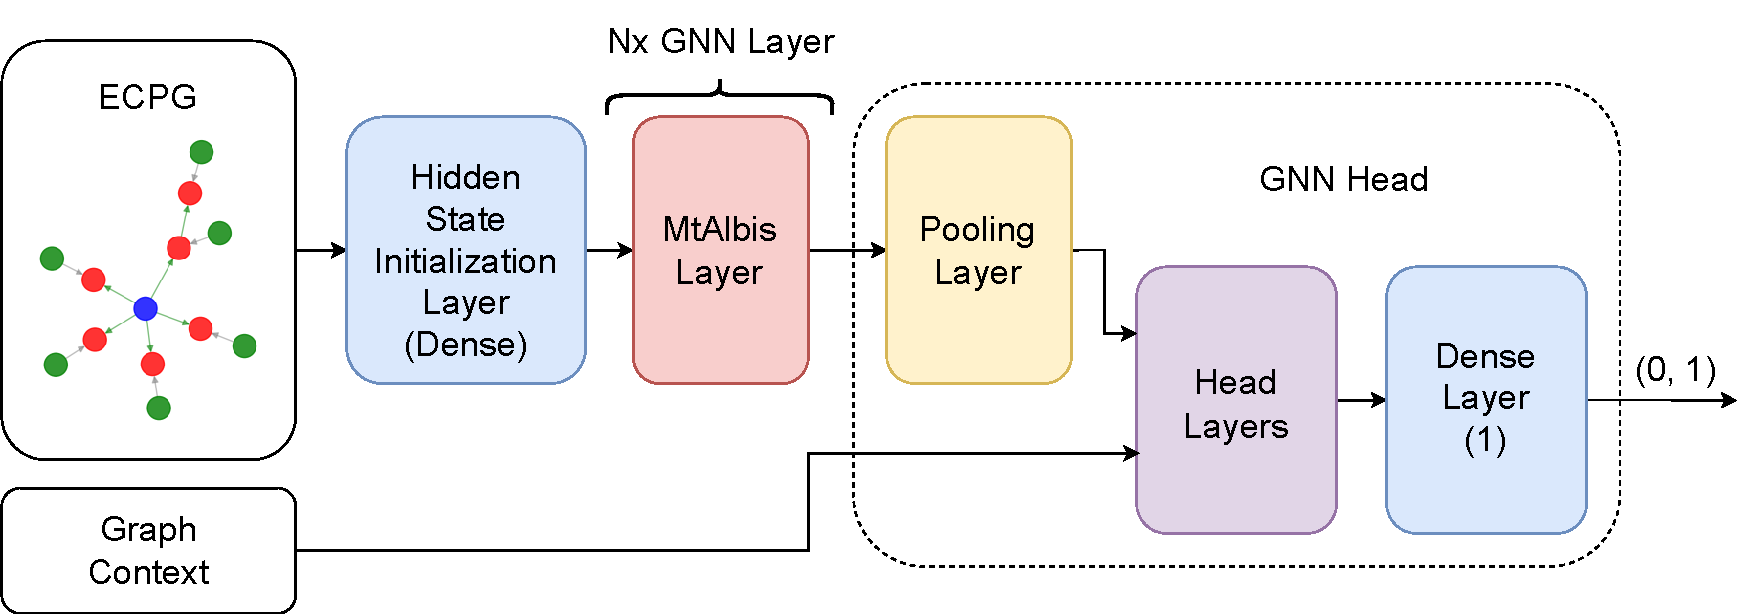
\includegraphics[width=1\textwidth]{figures/model-architecture.pdf}
	\caption{A~generalized architecture of the GNN models used in this thesis. The architecture is based on the MtAlbis GNN layers and is a binary classification model -- it ends with a Dense layer with a single output neuron.}
	\label{figure:model-architecture}
\end{figure}

The final part is the GNN head, which serves as the equivalent of the super node described in Section~\ref{gnn}. Information from all (or only some) node sets is input into a pooling layer, whose output is a combined hidden state (as it would be for a super node). This hidden state, together with features from the graph context, is input into additional fully connected layers (or a single layer), whose output is the model's output -- in this case, a single number. The model is supposed to distinguish between two classes, making it a binary classification. Thus, the last Dense layer must have a single neuron, as shown in Figure~\ref{figure:model-architecture}. The sigmoid function is applied to the output of this neuron (though it is not necessarily required), which converts the input number from the interval $(-\infty,+\infty)$ to $(0,1)$. Therefore, the model's output is a single number in this interval, which is higher the more confident the model is in class 1 (true positive). Models for binary classification are most often trained using \textit{Binary Cross Entropy}~\cite{cross-entropy}, as is the case with all models in this thesis.

Creating the training loop and saving models is again straightforward thanks to the use of TFGNN. Of course, it is also necessary to fine-tune hyperparameters such as learning rate, optimizer type, batch size, etc. More details can be found in Chapter~\ref{experiments}.

Models created using the training pipeline have interesting properties:
\begin{itemize}
    \item Thanks to the use of LLVM IR, they are \textbf{language-independent}.
    \item Since the output of Infer is only used for program slicing (and obtaining the type of error), it can \textbf{easily be adapted to another static analyzer}.
    \item It is also possible to use them \textbf{without a static analyzer}, if slicing criteria are created (possibly automatically) and the type of error is specified. This way, the models can completely replace static analysis and be used directly to find errors in the source code.
\end{itemize}


\section{Inference Pipeline}
\label{inference-pipeline}
The goal of the inference pipeline is to run Infer on a real C/C++ project, generate ECPGs for each Infer report, and then rank the reports based on their probability of being true positives using the created GNN models. As shown in Figure~\ref{figure:inference-pipeline}, the inference pipeline is fundamentally the same as the training pipeline. It differs only in the way LLVM bitcode is extracted and at the end, where models are not trained but are used solely for inference.

\begin{figure}[t]
	\centering
	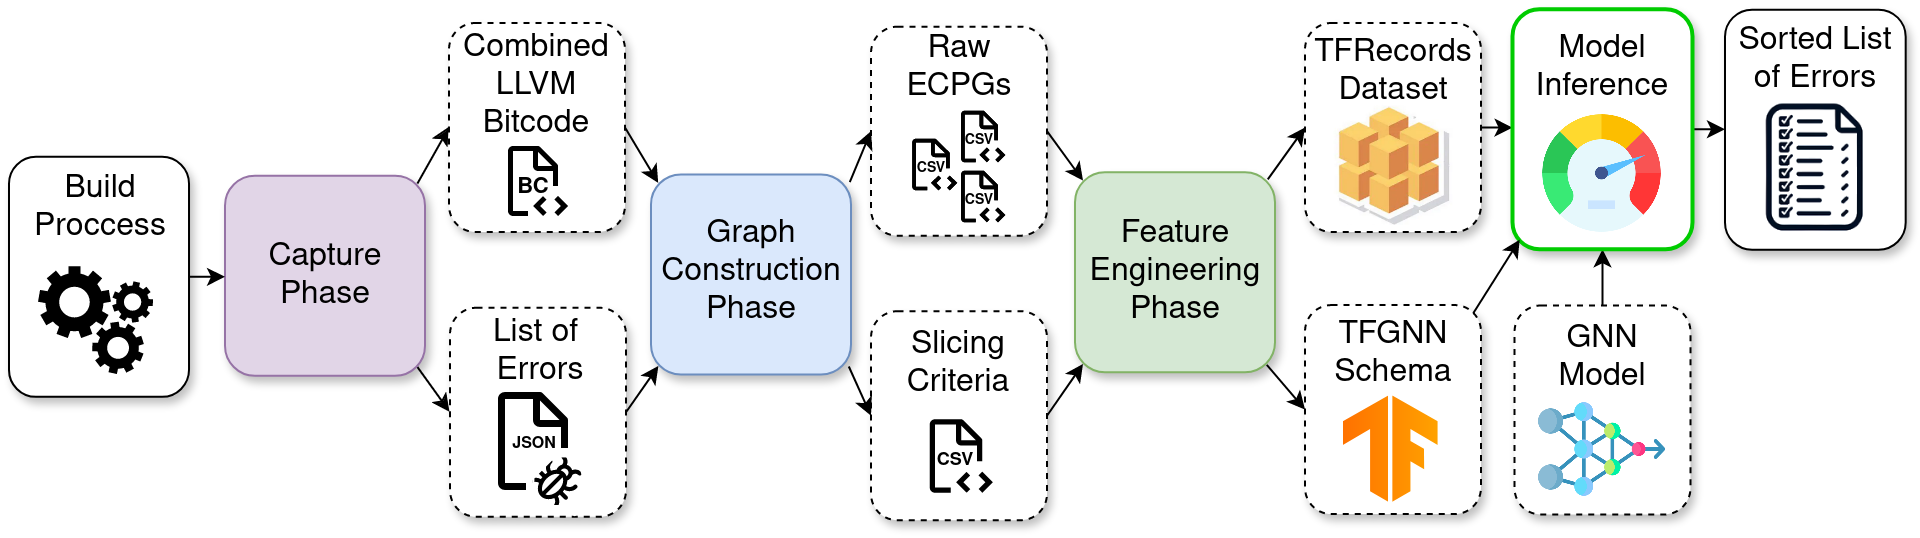
\includegraphics[width=1\textwidth]{figures/inference-pipeline.png}
	\caption{The figure shows a schematic of the inference pipeline, which ranks Infer reports on real C/C++ projects based on the probability of being true positives. The dashed boxes indicate the intermediate products and generated data. The green outline indicates tools created as part of this thesis. Icons were taken from~\cite{icon-model, icon-tfrecords, icon-inference}.}
	\label{figure:inference-pipeline}
\end{figure}

\subsection{Capture Phase}
\label{capture-phase}
The goal of the capture phase (see Figure~\ref{figure:capture-phase}) is to connect to a running build process and capture the information required for the graph construction phase (described in Section~\ref{graph-construction-phase}). This necessary information includes the source files compiled to LLVM bitcode and the same source files captured in Infer's capture phase (see Section~\ref{infer}), which will then be analyzed by Infer. To obtain this information, compilation commands must be extracted from the build process. This can be done by:
\begin{enumerate}
    \item parsing the build scripts,
    \item capturing the commands using a compiler wrapper.
\end{enumerate}

\begin{figure}[t]
	\centering
	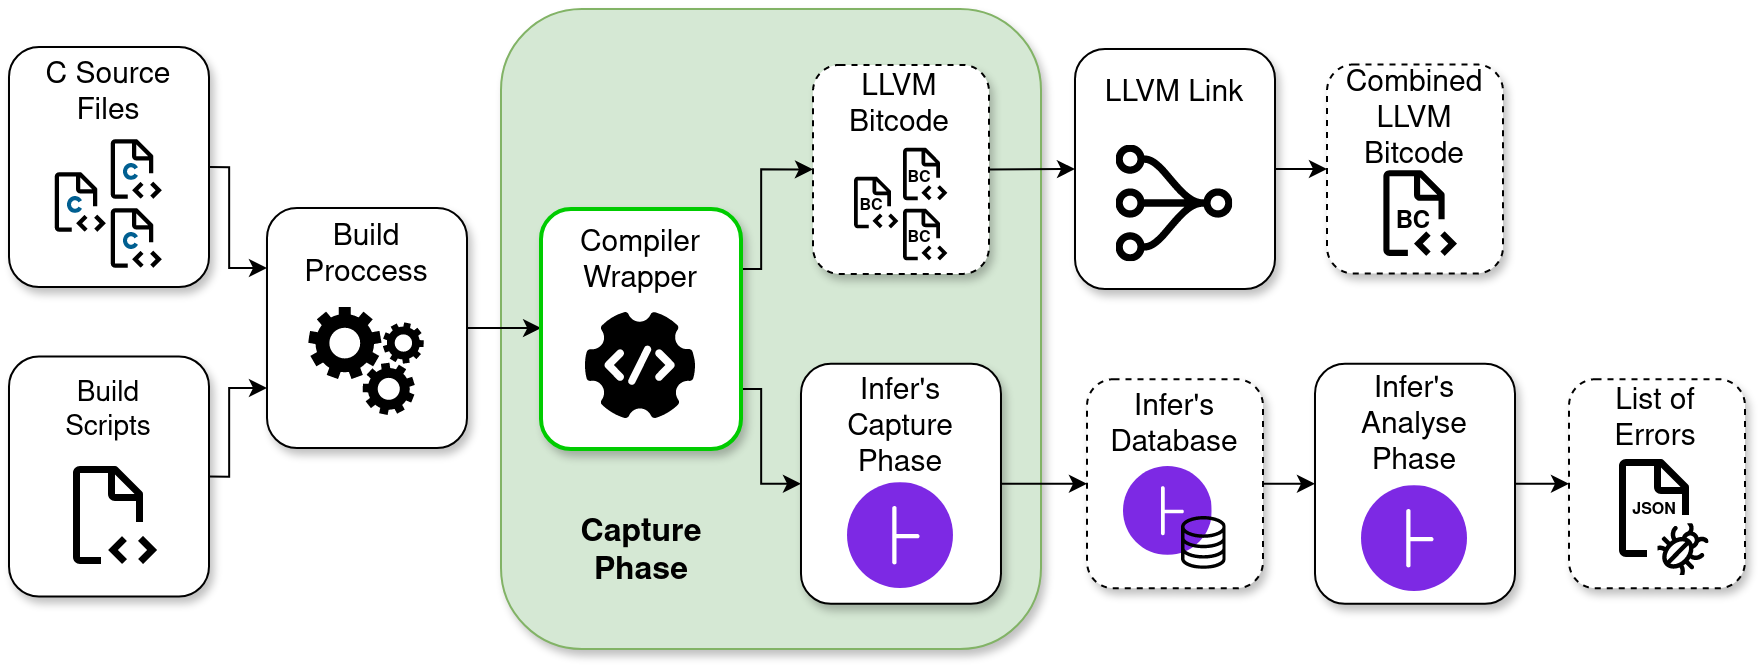
\includegraphics[width=1\textwidth]{figures/capture-phase.png}
	\caption{The figure shows a schematic of the capture phase, which generates LLVM bitcode and runs Infer analysis on real C/C++ software. The dashed boxes indicate the intermediate products and generated data. The green outline indicates tools created as a~part of this thesis. Icons were taken from~\cite{icon-compiler, infer-web}.}
	\label{figure:capture-phase}
\end{figure}

Parsing build scripts is very challenging because each build system uses a different syntax and different techniques. However, some build systems have built-in functionality for extracting compilation commands, such as CMake~\cite{cmake-doc}. Unfortunately, very few build systems have this feature. Another problem is that some software does not use any standard build systems. Instead, they use custom scripts (e.g., bash) for compilation, linking, etc. These scripts can have any structure and hierarchy of calling other scripts or tools, making it almost impossible to statically parse compilation commands from them. The use of such scripts is relatively common in SRPM\footnote{\textbf{Source Red Hat Package Manager (SRPM) package} -- provides the source code of software via the RPM package manager for operating systems like RHEL, Fedora, and CentOS.} packages, as found in author's previous work~\cite{bc}. This thesis aims for later deployment specifically on SRPM packages and must take this feature into account. For the reasons mentioned above, parsing build scripts of unknown software is generally impractical.

The second and practically applicable option is to create wrappers over C/C++ compilers and intercept the compilation commands during the build process. The design and implementation were addressed in the author's previous work~\cite{bc}, so the principles of the wrappers will be described here very briefly. Every time a compiler is invoked by the build system, the installed wrapper is called. For each such call, the wrapper captures its arguments and performs the following steps:

\begin{enumerate}
    \item It filters out options that are incompatible with Infer's internal Clang compiler, which is used to compile source files into SIL (see Section~\ref{infer}).
    \item It invokes Infer's capture phase, passing the modified compilation command. Infer then stores the captured source files in SIL representation in its database.
    \item It calls the original, unmodified command with the original compiler so that the build can proceed without issues.
\end{enumerate}

The wrapper is designed so that even if Infer's capture phase fails, the original command is still executed. Failure of Infer's capture phase will not crash the entire analysis/pipeline, but it may increase the likelihood of generating false positives/false negatives. This error recovery is possible due to Infer's properties: if it does not have the required implementations of the analyzed functions captured, it assumes they may return any value (limited by their return type, of course). This speculation introduces a certain degree of over-approximation and thus the potential for false positives. False negatives can occur because files not captured by the Infer capture phase are not analyzed. An important note is that these compiler wrappers can (and typically are) called in parallel. Therefore, it is necessary to be aware of possible critical sections, such as Infer's database. The description of how critical sections are protected in the wrapper can be found in~\cite{bc}.

For the inference pipeline, it is necessary to add additional functionality to the wrapper -- generating LLVM bitcode from each captured compilation command. The principle, including an example of how to generate LLVM bitcode using the compilation command, was already presented in Section~\ref{bitcode-generation}. Unlike the training pipeline, the inference pipeline must consider input compilation commands in all possible formats, so it is necessary to remove the \texttt{-o} option (and its value) and also ensure that it is truly a compilation command (it must contain the \texttt{-c} option).

The final task that the wrapper needs to accomplish is finding all the generated LLVM bitcode files. Again, there are several ways to obtain this list of files. For instance, one could analyze compilation commands and extract the names of the compiled files or insert \texttt{-o} options. However, the simplest method is currently used here: upon the wrapper's first invocation, a list of all existing \texttt{.bc} files in the filesystem is created. After the build is finished, this process is repeated. By comparing these two lists, it is possible to identify which \texttt{.bc} files were added during the build and thus contain the LLVM bitcode.

It may seem that running multiple builds concurrently could result in \texttt{.bc} files unrelated to the current project being compiled. This issue indeed occurs with all the methods mentioned, as it is not possible to distinguish which build the \texttt{.bc} files originated from. Similarly, Infer cannot distinguish between individual projects, so it is necessary to ensure that only one project's compilation is executed at any given time. However, running multiple projects concurrently will not cause errors but will merely lead to Infer reporting errors (and generating graphs) for all the projects being compiled.

After the build and before the graph construction phase begins, two additional steps must be taken. First, \textbf{all} generated LLVM bitcode files need to be merged into a~single file using the llvm-link tool. Then, the Infer analysis is performed on the captured files. After the analysis is complete, Infer generates a list of potential errors, from which slicing criteria are extracted for LLVM-Slicer during the graph construction phase. Unlike the training pipeline, where each error detected by Infer (or D2A sample in the training pipeline) generates its own LLVM bitcode file, here, a single file contains the entire source code. The LLVM bitcode files are differentiated only after slicing according to the criteria of individual reports.


\subsection{Inference Phase}
\label{inference-phase}
After the graph construction phase, feature engineering is applied to the raw ECPGs, just like in the training pipeline (see Section~\ref{feature-engineering}). The only difference is that normalization coefficients already generated from D2A are used.

Next comes the inference itself, as shown in Figure~\ref{figure:inference-pipeline}. The inference using the GNN model evaluates the input graphs -- representing individual errors found by Infer -- based on their probability of being true positives. The original output from Infer is then sorted in descending order according to the GNN model's score. Unsupported error types (see Section~\ref{bitcode-generation}) and errors for which a graph could not be generated (see Section~\ref{implementation}) are placed at the end of the list in their original relative order. Even in this sorted output, however, a typical trade-off is encountered between the number of true positives and the number of false positives. The more true positives that are sought, the worse the true positive vs. false positive ratio becomes (to ensure that all true positives are found, all reports must still be checked). However, the mere fact that it is possible to choose this threshold is a significant advantage of these sorted outputs compared to the unsorted ones.


\chapter{Implementation}
\label{implementation}
This chapter describes the implementation of training and inference pipelines, as designed in Chapter~\ref{design}. The training pipeline consists of a series of independent tools. Specifically, Section~\ref{implementation-d2a-filter} describes the D2A filter that removes unsupported error types. Section~\ref{implementation-bitcode-generator} discusses the implementation of a bitcode generator that creates LLVM bitcode for D2A samples. Section~\ref{implementation-slicing-info} describes the slicing criteria extractor. Section~\ref{implementation-graph-construction} details the generation of Graph D2A from LLVM bitcode. Section~\ref{implementation-norm-coeffs} explains the extraction of normalization coefficients for feature normalization. Section~\ref{implementation-feature-engineering} outlines the implementation of feature engineering, including graph and attribute transformations and normalization. Finally, Section~\ref{implementation-training} and Section~\ref{implementation-evaluation} cover model training and evaluation, respectively.

Unlike the training pipeline, the inference pipeline is fully automated. It comprises compiler wrappers, described in Section~\ref{implementation-compiler-wrapper}, and a script that automates graph creation, discussed in Section~\ref{implementation-inference-pipeline}.

All source files for both the training and inference pipelines are open-source and accessible on GitHub\footnote{All source files are available at \url{https://github.com/TomasBeranek/but-masters-thesis}.}. Data manipulation primarily utilized Python, particularly libraries such as Pandas\footnote{\textbf{Pandas}'s website: \url{https://pandas.pydata.org/}.}, NumPy\footnote{\textbf{NumPy}'s website: \url{https://numpy.org/}.}, NetworkX\footnote{\textbf{NetworkX}'s website: \url{https://networkx.org/}.} (nx), and TensorFlow\footnote{\textbf{TensorFlow}'s website: \url{https://www.tensorflow.org/}.}. Bash and make were used to automate the calling of scripts and other auxiliary tasks.

The following sections provide details on the computation times for various components. All measurements were conducted on Ubuntu 20.04 with the following hardware:
\begin{itemize}
    \item CPU\footnote{\textbf{Central Processing Unit (CPU).}} -- Intel(R) Core(TM) i5-10400F CPU @ 2.90GHz, 6x cores, 12x threads,
    \item GPU\footnote{\textbf{Graphics Processing Unit (GPU)}.} -- NVIDIA GeForce RTX 3060 Ti, 8GB,
    \item RAM\footnote{\textbf{Random Access Memory (RAM)}.} -- 16GB,
    \item Memory -- 500GB SSD\footnote{\textbf{Solid-State Drive (SSD)}.}.
\end{itemize}


\section{D2A Filter}
\label{implementation-d2a-filter}
The initial step in creating the Graph D2A involves filtering out unsupported data types, as discussed in Section~\ref{bitcode-generation}. This filtering is implemented through a script named \texttt{filter.py}, written for Python 3.8. The script takes a directory containing the D2A dataset as its input (specified using the \texttt{-d} or \texttt{-{}-dir} option), which can be downloaded from~\cite{D2A-webpage}. The files, named in the format \texttt{\{project\}\_labeler\_\{0|1\}.pickle.gz}, correspond to individual projects and labels. Although "after-fix" samples are available (see Chapter~\ref{chapter-d2a}), they are not used in this thesis and are ignored by \texttt{filter.py}. The second input parameter is the output directory (specified using the \texttt{-o} or \texttt{-{}-output-dir} option), where the results are stored (if the directory does not exist, it will be created).

Each input file in the input directory is first decompressed from the \texttt{.gz} archive using the \texttt{gzip} library. Then, using the \texttt{pickle} library, which is used for object serialization and deserialization, the samples are sequentially read. Samples belonging to the supported error types are saved in a file with the same name (including \texttt{.pickle.gz}) in the output directory. Unsupported samples are completely discarded.

From each saved sample, certain information that is no longer needed in the training pipeline is also removed. This significantly reduces the size of the samples, saving disk space and speeding up operations such as loading and saving. The removed information includes (explanations of each attribute can be found in~\cite{d2a-sample-description}) \texttt{label\_source}, \texttt{bug\_loc\_trace\_index}, \texttt{sample\_type}, \texttt{commit[changes]}, \texttt{functions}, and \texttt{zipped\_bug\_report}.

The command to run \texttt{filter.py} might look like this:
\begin{lstlisting}[language=bash, xleftmargin=2em]
python3.8 filter.py -d d2a/ -o d2a-filtered/
\end{lstlisting}

The script removes 20,732 samples with unsupported error types, which is \textasciitilde1.6~\% of the total number of samples. The number of removed samples for each project is shown in Table~\ref{tab:implementation-d2a}. Filtering the entire dataset takes \textasciitilde3 minutes, and the dataset size is reduced from \textasciitilde3.6GB to \textasciitilde288MB (calculated only with the \texttt{*\_labeler\_*} files).


\section{Bitcode Generator}
\label{implementation-bitcode-generator}
From the filtered D2A dataset, it is necessary to generate a single LLVM bitcode for each sample, as described in Section~\ref{bitcode-generation}. This is accomplished using the \texttt{generate\_bitcode.py} script for Python 3.8. The script must be applied individually to each \texttt{*\_labeler\_*} generated by \texttt{filter.py} (see Section~\ref{implementation-d2a-filter}), specified using the \texttt{-f} or \texttt{-{}-file} option. The script also requires the directory containing the \textbf{original} project repository (using the \texttt{-r} or \texttt{-{}-repository} option) and the project (using the \texttt{-{}-project} option) from which the LLVM bitcode will be generated, such as \texttt{httpd}\footnote{\textbf{httpd}'s repository: \url{https://github.com/apache/httpd}.}). Finally, the output directory must be specified (using \texttt{-o} or \texttt{-{}-output-dir}); if it does not exist, it will be created. Running \texttt{generate\_bitcode.py} might look as follows:
\begin{lstlisting}[language=bash, xleftmargin=2em]
python3.8 generate_bitcode.py -r httpd/ --project httpd \
-f d2a-filtered/httpd_labeler_1.pickle.gz -o d2a-bitcode/httpd_1/
\end{lstlisting}

The script first retrieves a chronological list of all commits from the repository using:
\begin{lstlisting}[language=bash, xleftmargin=2em]
git log --all --format=%H
\end{lstlisting}

Then, a set of commits for all samples from the input D2A file is obtained. From the complete list of commits, those that are not also in the set of commits from the D2A are removed -- in other words, commits on which no D2A samples exist. This modified list is reversed so that the first commit is the oldest and the last is the newest. The script then iterates through individual commits (represented by their hashes) and performs the following:

\begin{enumerate}
    \item The repository is switched to the given commit using \texttt{git reset -{}-hard HASH}.
    \item All files that are not part of the repository (especially products from previous runs) are deleted using \texttt{git clean -dfx}.
    \item A~project-specific set of actions required for a successful build is performed (see below).
    \item For each D2A sample at this commit:
    \begin{enumerate}
        \item A~list of files to be compiled for the given sample is obtained from D2A.
        \item Samples consisting only of \texttt{.h} files or containing files such as \texttt{.y} or \texttt{.l} are skipped, as they do not generate LLVM bitcode when compiled.
        \item The cache is checked to see if the LLVM bitcode for a sample with the same set of files has already been generated at the current commit. If so, a symlink\footnote{\textbf{Symlink} -- A~special type of file that points to another file in the filesystem.} \texttt{\{output\_dir\}/\{sample\_id\}.bc} is created, pointing to the already generated LLVM bitcode. This speeds up the process because recompilation is not required and reduces memory usage since the same sample does not need to be stored multiple times. Symlinks only occupy a few bytes.
        \item The repository is cleaned of residual files from previous compilations (at this commit) using project-specific criteria to avoid deleting essential configuration data generated when switching to this commit.
        \item A~set of already present \texttt{.bc} files in the repository is obtained; these are not LLVM bitcode files.
        \item For each record (compiled file) in the D2A attribute \texttt{compiler\_args}:
        \begin{enumerate}
            \item Adjust the D2A compiler arguments -- replace \texttt{<$repo$>} with the repository path and remove arguments starting with \texttt{<$sys$>}, which include external libraries specific to httpd (these libraries are included with their own paths, see below).
            \item Add missing project-specific include arguments (\texttt{-I}).
            \item Add arguments to generate LLVM bitcode (see Section~\ref{bitcode-generation}).
            \item Execute the generated compilation command.
        \end{enumerate}
        \item Using the previously located existing \texttt{.bc} files, obtain a list of newly added files -- generated LLVM bitcode files.
        \item Ensure that the same number of LLVM bitcode files have been generated as there are original \texttt{.c} files (\texttt{.h} files are included -- they do not generate separate LLVM bitcode).
        \item Use \texttt{llvm-link} to combine all LLVM bitcode files of the current sample into a~single LLVM bitcode file and save it to \texttt{\{output\_dir\}/\{sample\_id\}.bc}.
        \item Finally, note in the cache which files were used to generate this LLVM bitcode.
    \end{enumerate}
\end{enumerate}

After switching to the new version of the repository (new commit), a pre-compilation configuration is required. This typically involves generating platform-specific \texttt{.h} or \texttt{.c} files, generating configuration files, setting the correct paths to libraries, etc. This phase is different and quite extensive for each project, so only the procedure for httpd will be described here as an example. Configuration details of other projects can be found directly in \texttt{generate\_bitcode.py}.

The httpd project is the only one that requires downloading external libraries in advance. Specifically, \texttt{apr-1.7.4} and \texttt{apr-util-1.6.3}, which can be downloaded from the Apache website\footnote{\textbf{Apache}'s website: \url{https://apr.apache.org/download.cgi}.}, and the \texttt{pcre2-10.42} library, which is available in the \texttt{pcre2} repository\footnote{\textbf{pcre2}'s repository: \url{https://github.com/PCRE2Project/pcre2/releases/tag/pcre2-10.42}.}. These libraries must be renamed to \texttt{apr}, \texttt{apr-util}, and \texttt{pcre} and moved to the \texttt{httpd-dependencies/srclib} directory, which must be at the same level as the httpd repository. Furthermore, all libraries need to be configured according to their instructions (pre-configured libraries are included in the attached media; see Appendix~\ref{appendix-media}).

The \texttt{generate\_bitcode.py} script moves to the httpd repository and prepares for the httpd compilation as follows:
\begin{enumerate}
    \item Copies the external libraries \texttt{apr} and \texttt{apr-util} to the \texttt{srclib/} directory in the repository.
    \item In some versions of the repository that contain the \texttt{pcre} library, it is necessary to initiate configuration by first running \texttt{./buildconf} (still in the root directory of the repository), which creates \texttt{srclib/pcre/configure}. Then, switch to \texttt{srclib/pcre/} and run \texttt{./configure} to generate the necessary header files for the \texttt{pcre} library, such as \texttt{config.h}.
    \item If the \texttt{pcre} library is not present, the script copies the already configured one from \texttt{../httpd-dependencies/srclib/pcre/} into \texttt{srclib/}.
    \item The script then checks whether any of the tracked files have changed from the last version of the project:
    \begin{itemize}
        \item \texttt{include/ap\_config\_auto.h.in},
        \item \texttt{include/ap\_config\_layout.h.in},
        \item \texttt{modules/ssl/ssl\_policies.h.in},
        \item \texttt{buildconf}.
    \end{itemize}
    These are templates for the generated \texttt{.h} files and the configuration file. If none of these files have changed, the previously generated \texttt{.h} files can be reused -- copy them back from \texttt{/tmp/d2a\_pipeline/}. This saves a lot of time since generating them and running \texttt{./buildconf} is time-consuming across many commits.
    \item If any template has changed, \texttt{./buildconf} and \texttt{./configure} must be rerun. The configuration process takes about 20 seconds, but it has to be done for thousands of commits.
    \item The script checks another set of tracked files that are generated differently:
    \begin{itemize}
        \item \texttt{server/gen\_test\_char.c},
        \item \texttt{srclib/pcre/dftables.c}.
    \end{itemize}
    If they have not changed, again copy them from previous versions.
    \item If they have changed, they need to be generated as follows:
    \begin{enumerate}
        \item \texttt{include/test\_char.h} -- generated using \texttt{gcc -Isrclib/apr/include \newline -Isrclib/apr-util/include server/gen\_test\_char.c -o gen\_test\_char} 
        \newline followed by \texttt{./gen\_test\_char > include/test\_char.h}.
        \item \texttt{include/chartables.c} -- generated using \texttt{gcc srclib/pcre/dftables.c -o dftables} followed by \texttt{./dftables include/chartables.c}. In some newer versions, it is necessary to check if \texttt{include/chartables.c} was created, and if not, it must be generated using \texttt{./dftables > include/chartables.c} instead.
    \end{enumerate}
\end{enumerate}

For each version (commit) of the project, running the configuration multiple times should be avoided. To prevent losing the generated configuration files, a project-specific cleanup that preserves the contents of certain directories is used. For httpd, the command is:
\begin{lstlisting}[language=bash, xleftmargin=2em]
git clean -dfx --exclude=srclib/ --exclude=include/
\end{lstlisting}

When starting the compilation for individual files of each sample, arguments extracted from D2A are used. However, most are insufficient as they do not include necessary \texttt{-I} paths for various header files. This may be due to different methods of installing libraries when creating D2A, so these paths need to be added. For httpd, \texttt{-Iinclude}, \texttt{-Isrclib/apr/include}, and \texttt{-Isrclib/apr-util/include} are appended.

As previously indicated, some samples might be skipped, or their compilation may fail. Statistics for individual projects are presented in Table~\ref{tab:implementation-d2a}. For httpd\_1, the size of the filtered D2A is \textasciitilde47KB, compared to the unfiltered D2A, which is \textasciitilde629KB. The generated LLVM bitcode for httpd\_1 is \textasciitilde22MB. The script for \texttt{httpd\_1} runs for \textasciitilde330 seconds, which equates to \textasciitilde1.6 seconds per sample. Parallelization would speed this up, but since the project repository is a critical section accessed almost continuously, it would be necessary, for instance, to duplicate it. Thus, parallelization of this process is left for potential future improvements. Similarly, enhancements to the automated project configuration are also left for future improvements, as they could improve the success rate of bitcode generation. However, compilation issues must be resolved manually, which consumes an enormous amount of time.


\section{Slicing Criteria Extractor}
\label{implementation-slicing-info}
To enable slicing of the generated LLVM bitcode from Section~\ref{implementation-bitcode-generator}, it is first necessary to extract slicing criteria from the filtered D2A from Section~\ref{implementation-d2a-filter}. For this purpose, the Python 3.8 script \texttt{slicing\_criteria\_extraction.py} is provided. It takes as input a single file from the filtered D2A (specified using the \texttt{-{}-d2a} option). The script outputs the slicing criteria in the CSV format (without header) to \texttt{stdout}, with the following columns:

\begin{enumerate}
    \item \texttt{status} -- 0 means success, 1 indicates an internal error.
    \item \texttt{bug\_id} -- the \texttt{id} of the sample.
    \item \texttt{entry} -- name of the entry function (see Section~\ref{graph-construction-phase}).
    \item \texttt{file} -- the file where the error is located.
    \item \texttt{fun} -- the function where the error is located.
    \item \texttt{line} -- the line number where the error is located.
    \item \texttt{variable} -- the variable associated with the error.
\end{enumerate}

An example of running \texttt{slicing\_criteria\_extraction.py} might look like this:
\begin{lstlisting}[language=bash, xleftmargin=2em]
python3.8 slicing_criteria_extraction.py --d2a d2a-filtered/ \ 
httpd_labeler_1.pickle.gz > slicing-info/httpd_labeler_1.csv
\end{lstlisting}

The \texttt{slicing\_criteria\_extraction.py} script is used for both the training and inference pipelines. This is because both D2A and Infer's output are in the JSON format, and since D2A originates from Infer's output, they are quite similar. When the script is used on the D2A sample, it is converted to the same format as Infer's output via the simple \texttt{transform\_d2a\_sample} function, which essentially involves renaming and splitting some D2A attributes.

For each sample/report, a function \texttt{extract\_\{error\_type\_group\}} (extracting the slicing criteria) is invoked based on its type -- the 6 groups listed in Section~\ref{graph-construction-phase}. Retrieving \texttt{entry}, \texttt{file}, \texttt{fun}, and \texttt{line} is straightforward: the correct attributes are simply extracted from the JSON (see Section~\ref{graph-construction-phase}). If \texttt{variable} is extracted, it is obtained from the \texttt{qualifier} field. For \texttt{bug\_id}, \texttt{id} from D2A is used in the case of D2A. For Infer, the samples are labeled incrementally starting from \texttt{0}, and unsupported sample types are skipped in the numbering to preserve the original numbering in Infer's output.

The script skips unsupported error types. If an unknown format of a supported error is encountered, the script returns \texttt{status = 1} and tries to extract at least \texttt{entry}, \texttt{file}, \texttt{fun}, and \texttt{line} from the basic information to allow slicing based on the line number.

If the \texttt{file} is a header file (\texttt{.h}), the \texttt{file} field is left empty because of future slicing -- because slicing based on header files is not supported by LLVM-Slicer in the standard format. Instead, slicing should be done using only \texttt{fun} and \texttt{line}, excluding the \texttt{file} field. If the \texttt{file} contains a regular \texttt{.c} file, \texttt{fun} is omitted because \texttt{file} and \texttt{line} are sufficient to determine the slicing criteria unambiguously. Extracting slicing criteria from the filtered D2A completes for all files in under a minute.


\section{Graph Construction Script}
\label{implementation-graph-construction}
The bash script \texttt{construction\_phase\_d2a} is used for generating Graph D2A from LLVM bitcode (created in Section~\ref{implementation-bitcode-generator}) and slicing criteria in the CSV format (created in Section~\ref{implementation-slicing-info}). This script implements the remaining transformations described in Section~\ref{graph-construction-phase}. The script accepts the following position-dependent arguments:
\begin{enumerate}
    \item The output directory for storing raw ECPGs.
    \item The file containing slicing criteria.
    \item The directory containing LLVM bitcode.
    \item (optional) The sample number at which to end.
    \item (optional) The sample number from which to start.
\end{enumerate}

The \texttt{construction\_phase\_d2a} script can be executed with a command such as:
\begin{lstlisting}[language=bash, xleftmargin=2em]
./construction_phase_d2a graph-d2a/httpd_1 httpd_labeler_1.csv \
d2a-bitcode/httpd_1
\end{lstlisting}

The script \texttt{construction\_phase\_d2a} operates as follows:
\begin{enumerate}
    \item Records from the slicing information (from its copy) that already have a directory with raw ECPG are removed. This allows for the intermittent transformation of the dataset.
    \item The slicing information file is divided into smaller files of 100 lines each (the last file may be smaller) and stored in \texttt{/tmp/construction\_phase\_d2a/split\_files/}.
    \item Each file in \texttt{split\_files/} is then processed as follows:
    \begin{enumerate}
        \item The \texttt{create\_cpgbin} function is called in parallel for each line in \texttt{file} using the command:
\begin{lstlisting}[language=bash, xleftmargin=1em]
cat ${file} | parallel --colsep ',' create_cpgbin {1} {2} {3} \
{4} {5} {6} {7}
\end{lstlisting}
        This function generates a binary CPG for each line from LLVM2CPG (detailed description of this function is provided below).
        \item If \texttt{/tmp/construction\_phase\_d2a/cpg/\$\{bug\_id\}.cpg.bin.zip} was not generated for some samples, these samples are removed from \texttt{file}.
        \item A script for Joern is generated, containing commands to load and re-save all \texttt{.cpg.bin.zip} files, thereby expanding them into ECPGs. An example Joern script is provided in Listing~\ref{listing:joern-script}.
        \item Joern processes all (up to 100) ECPGs.
        \item The \texttt{cpgbin\_to\_csv} function is called in parallel for each line in \texttt{file}, but only the \texttt{bug\_id} column is used:
\begin{lstlisting}[language=bash, xleftmargin=1em]
cat ${file} | parallel --colsep ',' cpgbin_to_csv {2}
\end{lstlisting}
        This function converts binary ECPGs to CSV -- raw ECPGs, stored in the output directory. Each raw ECPG has its own directory (named after its \texttt{bug\_id}) containing CSV files.
        \item Finally, all temporary files created during the current iteration are cleaned up to prevent accumulation of logs and intermediate files, which could unnecessarily consume memory.
    \end{enumerate}
    \item Statistics on the number of successful/unsuccessful samples are then calculated and printed.
\end{enumerate}

\begin{lstlisting}[
    language=json, 
    label={listing:joern-script}, 
    float=t,
    caption={An example of an automatically generated Joern script for \texttt{httpd\_1}. The script only includes \texttt{importCpg} to load binary CPGs (up to 100) and concludes with the \texttt{save} command, which saves the graphs.}
]
 importCpg("/tmp/construction_phase_d2a/cpg/httpd_27 ... 17_1.cpg.bin.zip")
 importCpg("/tmp/construction_phase_d2a/cpg/httpd_04 ... 1e_1.cpg.bin.zip")
 // more imports
 importCpg("/tmp/construction_phase_d2a/cpg/httpd_3e ... 2c_1.cpg.bin.zip")
 importCpg("/tmp/construction_phase_d2a/cpg/httpd_1d ... 02_1.cpg.bin.zip")
 save
\end{lstlisting}

The aforementioned function \texttt{create\_cpgbin}, which takes a line with slicing criteria as input, works as follows:
\begin{enumerate}
\item First, it checks whether the input directory with LLVM bitcode contains the bitcode for the current sample. If it does, the function continues.
\item The LLVM-Slicer is called using:
\begin{lstlisting}[language=bash, xleftmargin=1em]
timeout 3s llvm-slicer --sc="${file}#${fun}#${line}#${variable}" \
--entry=${entry} -o=${bc_sliced} ${bc_combined}
\end{lstlisting}
The \texttt{timeout} command ensures that \texttt{llvm-slicer} completes its run. Experiments have shown that it can sometimes get stuck or run for several minutes, which is unacceptable given the large number of samples. By removing certain columns from the slicing criteria (see Section~\ref{implementation-slicing-info}) and leveraging the behavior of variables in bash, it is possible to call \texttt{llvm-slicer} uniformly for both \texttt{.c} and \texttt{.h} files.
\item If \texttt{llvm-slicer} is successful, a CPG in binary format is generated using \texttt{llvm2cpg} as follows:
\begin{lstlisting}[language=bash, xleftmargin=1em]
llvm2cpg ${bc_sliced} --output=${cpg_bin}
\end{lstlisting}
where \texttt{\$\{cpg\_bin\}=/tmp/construction\_phase\_d2a/cpg/\$\{bug\_id\}.cpg.bin.zip}.
\end{enumerate}

The \texttt{cpgbin\_to\_csv} function, which takes only \texttt{bug\_id} as input, simply calls \texttt{joern-export} as follows:

\begin{lstlisting}[language=bash, xleftmargin=2em]
joern-export --repr all --format neo4jcsv \
-o "${output_dir}/${bug_id}" ${joern_cpg_bin}
\end{lstlisting}

where \texttt{\$\{joern\_cpg\_bin\}} contains the path to the binary ECPG in the temporary directory \texttt{/tmp/construction\_phase\_d2a/workspace/\$\{bug\_id\}.cpg.bin.zip/cpg.bin}. At the end of the function, the success of \texttt{joern-export} is checked.

As mentioned earlier, the creation of binary CPGs and the conversion of binary ECPGs to CSV are parallelized using the \texttt{parallel} tool. However, the bottleneck here is Joern, which, despite running multiple instances, does not provide any speedup. Moreover, starting up Joern takes multiple seconds, so ideally, it is best to start and stop it as little as possible, hence it works in batches of 100. Larger batch sizes have been tested to further reduce the startup load of Joern, but the following issues were found:
\begin{itemize}
\item Batch > 5000 -- Joern crashes.
\item Batch > 3000 -- Joern may get stuck in an infinite loop.
\item Batch > 500 -- Joern non-deterministically generates incomplete graphs (missing edge sets like \texttt{CDF}, \texttt{CFG}, etc.).
\item Batch = 100 -- Joern works correctly.
\end{itemize}

The following results were measured on \texttt{httpd\_1}. The non-parallelized script generates approximately 500 graphs per hour. By parallelizing both of the phases mentioned above, the script reaches approximately 1100 graphs per hour. Moving Joern to batch mode allows the script to generate approximately 4000 graphs per hour. Other projects have been found to contain, on average, larger graphs than \texttt{httpd}, so the number of graphs per hour may be smaller for those projects. The output graphs for httpd\_1 are \textasciitilde240MB.

As hinted earlier, some samples may fail. The largest contributing factor is the timeout for LLVM-Slicer. It is possible to increase the timeout, but that would decrease the number of graphs per hour. The number of successfully generated samples can be seen in Table~\ref{tab:implementation-d2a}.


\section{Normalization Coefficients Extractor}
\label{implementation-norm-coeffs}
Before applying feature engineering (see Section~\ref{feature-engineering}), it is necessary to extract normalization coefficients from individual projects in Graph D2A (created in Section~\ref{implementation-graph-construction}). This is the task of the \texttt{find\_normalization\_coefficients.py} script for Python 3.8. The script is executed for each project separately with 6 position-dependent arguments:
\begin{enumerate}
    \item directory with false positives in Graph D2A of the specific project,
    \item directory with true positives in Graph D2A of the specific project,
    \item project name (httpd, nginx, or libtiff),
    \item \texttt{splits.csv} file providing the data split into train, val, and test sets, downloadable from~\cite{D2A-webpage},
    \item slicing criteria for false positives of the specific project,
    \item slicing criteria for true positives of the specific project.
\end{enumerate}
Running the \texttt{find\_normalization\_coefficients.py} script for httpd could look like this:
\begin{lstlisting}[language=bash, xleftmargin=2em]
python3.8 find_normalization_coefficients.py graph-d2a/httpd_0/ \
graph-d2a/httpd_1/ httpd d2a/splits.csv httpd_labeler_0.csv \
httpd_labeler_1.csv
\end{lstlisting}

The \texttt{find\_normalization\_coefficients.py} script works as follows:
\begin{enumerate}
    \item It processes \texttt{splits.csv} and selects the set of \texttt{id} samples belonging to the input project and the training set.
    \item It then iterates over all false positive samples and then all true positive samples (the order does not matter) as follows:
    \begin{enumerate}
        \item If the sample \texttt{id} is not in the training set, it is skipped -- obtaining information from the validation and test sets is avoided because it could affect the experiments.
        \item For each CSV header file (\texttt{*\_header.csv}) of the current sample:
        \begin{enumerate}
            \item If the current header file does not belong to the original node sets of the merged node set \texttt{AST\_NODE} (see Section~\ref{feature-engineering}), the node set \texttt{TYPE}, or the node set \texttt{MEMBER}, proceed to the next header file.
            \item The corresponding data file \texttt{*\_data.csv} is read.
            \item If the header is \texttt{nodes\_TYPE\_header.csv} (\texttt{TYPE} node set), \texttt{LEN} and \texttt{PTR} values are extracted (see Section~\ref{feature-engineering}) and if their maximum values are greater than the currently found ones, they are updated. Then, proceed to the next header file.
            \item For a header file from the merged \texttt{AST\_NODE} node set or \texttt{MEMBER} node set, the values \texttt{MEMBER\_ORDER} (for node set \texttt{MEMBER}) and \texttt{ORDER} (for all others) are updated (see Section~\ref{feature-engineering}).
            \item If the header file is for the node set \texttt{METHOD}, newly found operators (if any) are added to the \texttt{OPERATORS} set.
            \item If the header file has a column \texttt{ARGUMENT\_INDEX}, it is stored together with the column \texttt{ID}.
        \end{enumerate}
        \item From the file \texttt{edges\_ARGUMENT\_data.csv}, obtain the set of target nodes for \texttt{ARGUMENT} edges. From previously stored \texttt{ARGUMENT\_INDEX}, discard those that are not target nodes for \texttt{ARGUMENT} edges (using \texttt{ID}s). From the remaining ones, update the maximum value of \texttt{ARGUMENT\_INDEX}.
    \end{enumerate}
    \item Extract the maximum value of \texttt{LINE} (for graph context, see Section~\ref{gnn-model}) from the files with slicing criteria.
    \item Finally, print all normalization coefficients.
\end{enumerate}

The \texttt{find\_normalization\_coefficients.py} script outputs its results to \texttt{stdout} in the format shown in Listing~\ref{listing:norm-coeffs}. Normalization coefficients \texttt{ARGUMENT\_INDEX}, \texttt{LEN}, \texttt{LINE}, \texttt{ORDER}, \texttt{MEMBER\_ORDER} and \texttt{PTR} are the maxima of all found attributes. \texttt{OPERATORS} is the set of all found operators. And \texttt{BUG\_TYPES} is the set of all supported error types (see Section~\ref{bitcode-generation}). Extraction for the httpd project takes about \textasciitilde260s.


\begin{lstlisting}[
    language=json, 
    label={listing:norm-coeffs}, 
    float=t,
    caption={An example of the normalization coefficients for the httpd project, generated by the \texttt{find\_normalization\_coefficients.py} script.}
]
 {'ARGUMENT_INDEX': 14,
  'BUG_TYPES': ['NULL_DEREFERENCE',
                // more error types
                'UNINITIALIZED_VALUE'],
  'LEN': 65536,
  'LINE': 9162,
  'MEMBER_ORDER': 75,
  'OPERATORS': {'<operator>.addition',
                '<operator>.addressOf',
                // more operators
                '<operator>.subtraction',
                '<operator>.xor'},
  'ORDER': 1471,
  'PTR': 4}
\end{lstlisting}


\section{Feature Engineering Script}
\label{implementation-feature-engineering}
After extracting the normalization coefficients (described in Section~\ref{implementation-norm-coeffs}), feature engineering (designed in Section~\ref{feature-engineering}) can be applied to Graph D2A (created in Section~\ref{implementation-graph-construction}) to produce a dataset in the TFRecords format. All feature selection, graph transformations, and attribute transformations are implemented using the \texttt{feature\_engineering.py} script for Python 3.8. The script is called separately for each project and label with 8 position-dependent arguments:
\begin{enumerate}
    \item TFGNN schema file (designed in Section~\ref{feature-engineering}),
    \item output file name,
    \item project name (httpd, libtiff, nginx, ...),
    \item label (\texttt{0} or \texttt{1}),
    \item \texttt{splits.csv} file,
    \item filtered D2A file (\texttt{*\_labeler\_*}),
    \item file with slicing criteria,
    \item (optional) Which of the normalization coefficients to use (\texttt{httpd}, \texttt{libtiff}, \texttt{nginx}, or \texttt{nginx+libtiff+httpd}). If the argument is missing, the project value is used.
\end{enumerate}

The script reads directories with individual samples from its \texttt{stdin} (one directory per line). Running \texttt{feature\_engineering.py} for \texttt{httpd\_1} might look like this:
\begin{lstlisting}[language=bash, xleftmargin=2em]
find graph-d2a/httpd_1 -mindepth 1 -type d | python3.8 \
feature_engineering.py extended_cpg.pbtxt \
tfrecords/httpd_1.tfrecords httpd 1 d2a/splits.csv \
d2a-filtered/httpd_labeler_1.pickle.gz httpd_labeler_1.csv
\end{lstlisting}

The \texttt{feature\_engineering.py} script does the following for each input Graph D2A sample:
\begin{enumerate}
    \item Loads only those node/edge set files that are not to be removed, with the exception of the \texttt{TYPE\_DECL} node set, which is removed later (see Section~\ref{feature-engineering}). If any used edges were connected to a node that was not loaded, it becomes an invalid node that needs to be removed appropriately. During loading, a merged \texttt{AST\_NODE} is also created, and the original node set name is stored in the \texttt{LABEL} attribute of each \texttt{AST\_NODE} node.
    \item Discards unused node set attributes.
    \item From the loaded nodes and the \texttt{AST} node set, a \texttt{MultiDiGraph} representation is created using the \texttt{nx} library optimized for graph processing.
    \item Using the simple algorithm described in Section~\ref{feature-engineering}, all invalid nodes are removed from the graph (for now, it is just a set of ASTs).
    \item Using \texttt{nx.weakly\_connected\_components(G)}, all WCCs are obtained, and those consisting only of \texttt{BLOCK} nodes are removed.
    \item All leaf \texttt{BLOCK} nodes are also removed. At this stage, all currently present nodes are considered valid (although some will still be removed later).
    \item Other edge sets are added to the graph, with the \texttt{ARGUMENT} edges only added if they originate from a \texttt{CALL}, meaning:
\begin{lstlisting}[language=bash, xleftmargin=2em]
G.nodes[edge['start']]['type'] == 'CALL'
\end{lstlisting}
    \item Newly added edges may again create invalid nodes, which can now be easily removed along with their edges, as removing them will not disconnect the ASTs.
    \item The graph optimizations described in Section~\ref{feature-engineering} are then performed:
    \begin{enumerate}
        \item removing AST children of external methods,
        \item removing unnecessary \texttt{EVAL\_TYPE} edges,
        \item removing all \texttt{TYPE\_DECL} nodes,
        \item removing unused \texttt{TYPE} nodes.
    \end{enumerate}
    \item At this stage, it is verified that the graph forms a single WCC because no further edge or node removals will be performed that could split the graph into multiple WCCs.
    \item All \texttt{METHOD} and \texttt{LITERAL} nodes are split into data and latent nodes (see Section~\ref{feature-engineering}), which adds the node sets \texttt{METHOD\_INFO}, \texttt{LITERAL\_VALUE}, and also the edge sets \texttt{METHOD\_INFO\_LINK} and \texttt{LITERAL\_VALUE\_LINK}.
    \item At this stage, all node/edge sets are converted to separate \texttt{DataFrame} tables using the \texttt{Pandas} library, which is optimized for tabular operations. From this point onward, attributes of individual edge/node sets are processed in groups, not the graph structure itself.
    \item All attributes are split as needed and normalized using the extracted normalization coefficients (see Section~\ref{feature-engineering}).
    \item Now, it is necessary to convert \texttt{SOURCE} and \texttt{TARGET}, which contain the node IDs in all edges. Currently, nodes have IDs in ascending order starting from 1. However, TFGNN identifies nodes differently. They are numbered in ascending order starting from 0, but within node sets -- meaning there can be two or more nodes with the same ID if each is in a different node set. Since edge sets must define source and target node sets (see Section~\ref{feature-engineering}), there will be no collisions.
    \item Finally, the orientation of some edge sets is reversed (see Section~\ref{feature-engineering}).
    \item A~TFGNN \texttt{GraphTensor} is created using the \texttt{from\_pieces} and \texttt{from\_fields} methods~\cite{tfgnn-graphtensor},
    \item Serializes the \texttt{GraphTensor} objects into \texttt{tfrecords} files according to whether the sample belongs to the train, val, or test set.
\end{enumerate}

The outputs of the \texttt{feature\_engineering.py} script are files with the \texttt{*.train}, \texttt{*.val}, and \texttt{*.test} extensions in the TFRecords format. Some samples may be faulty -- for instance, no \texttt{AST} edge set was generated for them (by Joern), which must always be present in a valid sample. The number of successfully generated samples is shown in Table~\ref{tab:implementation-d2a}. The script runs on \texttt{httpd\_1} for approximately \textasciitilde80 seconds. The script was parallelized at the level of individual samples, but parallelization did not bring any significant speed improvement (likely because the libraries used are already internally parallelized), and some calls to the TensorFlow library (e.g., writing to TFRecords) did not work and would need to be locked into critical sections. Therefore, the parallelization was removed. The output TFRecords files for httpd\_1 are \textasciitilde15MB.

\begin{lstlisting}[
    language=python, 
    label={listing:convert-id}, 
    float=t,
    caption={An example of Python code that converts Joern node IDs into TFGNN IDs.}
]
 for edge_set_name, val in edgeset_info.items():
     source_nodeset=val['SOURCE']
     target_nodeset=val['TARGET']

     get_source_node_loc = lambda id: graph_in_dfs[source_nodeset].index.get_loc(id)
     get_target_node_loc = lambda id: graph_in_dfs[target_nodeset].index.get_loc(id)

     graph_in_dfs[edge_set_name]['source']=graph_in_dfs[edge_set_name] \      
       ['source'].apply(get_source_node_loc)
     graph_in_dfs[edge_set_name]['target']=graph_in_dfs[edge_set_name] \
       ['target'].apply(get_target_node_loc)
\end{lstlisting}

\begin{table}
    \centering
    \caption{The table shows the number of samples after each phase of the training pipeline. For values marked with *, the loss is not final as they were not transformed into TFRecords. However, the table indicates that this final transformation is almost lossless.}
    \vskip6pt
    \begin{tabular}{!{\vrule width 1pt}l!{\vrule width 1pt}r|r|r|r|r!{\vrule width 1pt}r!{\vrule width 1pt}}
        \noalign{\hrule height 1pt}
        {\small \textbf{Project}} & {\small \textbf{D2A}} & {\small \textbf{Filtered D2A}} & {\small \textbf{Bitcode}} & {\small \textbf{Graph D2A}} & {\small \textbf{TFRecords}} & {\small \textbf{Loss}} \\
        \noalign{\hrule height 1pt}
        httpd\_0 & 12475 & 11974 & 11818 & 9705 & 9705 & 22 \% \\ \hline
        httpd\_1 & 217 & 210 & 210 & 193 & 193 & 11 \% \\ \hline
        nginx\_0 & 17945 & 17209 & 17172 & 16741 & 16741 & 7 \% \\ \hline
        nginx\_1 & 421 & 418 & 417 & 407 & 407 & 3 \% \\ \hline
        libav\_0 & 236415 & 234062 & 226213 & 186614 & 186595 & 21 \% \\ \hline
        libav\_1 & 4614 & 4575 & 4398 & 3331 & 3331 & 28 \% \\ \hline
        libtiff\_0 & 12096 & 11385 & 11377 & 9276 & 9276 & 23 \% \\ \hline
        libtiff\_1 & 553 & 534 & 534 & 459 & 459 & 17 \% \\ \hline
        openssl\_0 & 343148 & 332584 & 301934 &  278292 & - & 20 \%* \\ \hline
        openssl\_1 & 8022 & 7913 & 7581 & 6918 & - & 14 \%* \\ \hline
        ffmpeg\_0 & 654891 & 649255 & 633997 & 500791 & - & 24 \%* \\ \hline
        ffmpeg\_1 & 4826 & 4772 & 4621 & 3938 & - & 18 \%* \\ \hline
        \noalign{\hrule height 1pt}
    \end{tabular}
    \label{tab:implementation-d2a}
\end{table}


\section{Model Training Script}
\label{implementation-training}
After creating TFRecords files, training of GNN models can be done using the script \texttt{mixed\_nodes\_model.py} for Python 3.8. This script takes 4 position-dependent arguments:
\begin{enumerate}
    \item TFGNN schema,
    \item directory with TFRecords,
    \item output directory for saving models,
    \item (optional) the value \texttt{combined} to train a single model across multiple projects (see Section~\ref{hyperparameter-tuning}); if omitted, a separate model is trained for each project.
\end{enumerate}

The script \texttt{mixed\_nodes\_model.py} trains models on training data (and validates on validation data) of the projects httpd, libtiff, and nginx. It expects files named according to the pattern:
\begin{lstlisting}[language=bash, xleftmargin=2em]
{TFRecords_dir}/{httpd|libtiff|nginx}_{0|1}.tfrecords.{train|val}
\end{lstlisting}
The script then operates as follows:
\begin{enumerate}
    \item Data are loaded using \texttt{tf.data.TFRecordDataset} -- positive and negative samples separately (validation data are loaded all at once, as shuffling is not necessary).
    \item Up-sampling is applied to the minority class.
    \item Positive and negative samples are interleaved.
    \item All samples are shuffled to mix the samples from the individual projects.
    \item Datasets are batched.
    \item A \texttt{preprocessing} model is applied, which extracts the labels (see Section~\ref{gnn-model}).
    \item The function \texttt{train\_model} is then called, performing:
    \begin{enumerate}
        \item First, a model is constructed using the \texttt{build\_model} function, which utilizes the Keras API\footnote{\textbf{Keras API}'s documentation: \url{https://www.tensorflow.org/guide/keras}.} and operates as follows:
        \begin{enumerate}
            \item An \texttt{Input} layer is created, taking graphs defined by the TFGNN schema as input.
            \item A \texttt{Dense} layer initializing hidden states for each node set (and optionally edge sets) is added, using \texttt{MapFeatures}.
            \item GNN layers \texttt{mt\_albis.MtAlbisGraphUpdate} are added.
            \item A \texttt{Pool} layer is added.
            \item \texttt{Dense} layers in the GNN head are added, combining context features and the output of the \texttt{Pool} layer.
            \item Finally, a \texttt{Dense} layer with a single output and sigmoid activation function is added.
        \end{enumerate}
        \item The loss function, metrics, and optimizer are set, and the model is compiled using \texttt{model.compile}.
        \item An \texttt{EarlyStopping} callback monitoring Area Under the Receiver Operating Characteristic Curve (AUROCC) (see Section~\ref{base-model}) on validation data is set.
        \item Finally, the training loop is initiated using \texttt{model.fit}.
    \end{enumerate}
    \item Thanks to the \texttt{EarlyStopping} callback, the output of the training is the model with the highest validation AUROCC found. This model (or models) is then saved to the output directory. Directories with models are automatically saved with the prefix \texttt{\{ID\}\_}, where \texttt{ID} is a unique number -- the largest found in the directory, increased by one. The directory name might look like \texttt{8\_AUC\_0.818}, where the AUC value specifically refers to the validation AUROCC (or their average in case of multiple models). The values of hyperparameters set in the dictionary \texttt{hyperparameters} are stored in the output folder in the file \texttt{hyperparameters.json}.

\end{enumerate}

The entire model architecture is defined in the \texttt{build\_model} function. Older versions of this script for earlier models can be found in the repository under commits named \texttt{Model \{ID\} - AUC 0.XYZ}. These historical versions, though executable, do not represent the final form of the training script and should only be used for insight into the architecture definition.

\section{Model Evaluation Script}
\label{implementation-evaluation}
Trained models can be evaluated using the \texttt{evaluate\_model.py} script for Python 3.8. The models are evaluated based on two metrics -- AUROCC and Top N~\% Precision (see Section~\ref{model-comparison}). Examples of these for the libtiff project and top-performing models are shown in Figure~\ref{figure:auc-libtiff} and Figure~\ref{figure:topn-libtiff}, respectively. The script accepts 5 position-dependent arguments:
\begin{enumerate}
    \item TFGNN schema,
    \item directory with TFRecords files,
    \item directory with saved models,
    \item model \texttt{ID},
    \item dataset type -- \texttt{test}, \texttt{val}, or \texttt{train}.
\end{enumerate}

The script initially loads the data in the TFRecords format from the same location and with the same naming convention as used by \texttt{mixed\_nodes\_model.py} (see Section~\ref{implementation-training}), with additional \texttt{*.test} files. No data shuffling or modifications are required for the evaluation. A~preprocessing model is applied to extract labels from the graphs. Then, the model (or models) is loaded using \texttt{tf.keras.models.load\_model}, and inference is performed on the data using \texttt{model.predict}. The results are provided to the \texttt{plot\_top\_N\_precision} function, which plots the precision dependency on the number of top-selected samples. Additionally, the \texttt{plot\_ROC\_curve} function is called to create ROC curves. Both graphs are displayed and also saved in the current directory under the names \texttt{ROC\_curves.svg} and \texttt{Top\_N\_precisions.svg}.

The script can be run in a special mode that creates graphs for predefined scenarios (all graphs in Chapter~\ref{experiments} were created using these scenarios), by passing the following special model \texttt{ID} values (4th argument):
\begin{enumerate}
    \item \texttt{combined} -- testing top performing models from Section~\ref{model-comparison} on combined data from the httpd, libtiff, and nginx projects.
    \item \texttt{httpd} -- testing top performing models on httpd.
    \item \texttt{libtiff} -- testing top performing models on libtiff.
    \item \texttt{nginx} -- testing top performing models on nginx.
    \item \texttt{libav} -- testing top performing models on libav -- this involves cross-analysis. Files \texttt{libav\_\{0|1\}.tfrecords.\{train|test|val\}} are required.
    \item \texttt{chatgpt} -- comparing the top performing model with ChatGPT4 (see Section~\ref{comparison-chatgpt}). The file \texttt{libtiff-chatgpt.tfrecords.test}, containing selected samples, is needed.
\end{enumerate}



\section{Compiler Wrapper}
\label{implementation-compiler-wrapper}
The compiler wrapper originates from the author's previous work~\cite{bc}, where its implementation is also described. Here, only a brief overview will be provided, focusing mainly on its inputs and outputs for integration with other parts of the inference pipeline.

The compiler wrapper is a bash script that replaces C/C++ compilers, and the original compiler binaries are renamed to \texttt{\{compiler\}-original} (e.g., \texttt{gcc} becomes \texttt{gcc-original}). The repository includes a \texttt{Makefile}\footnote{\textbf{Makefile for installing wrappers}: \url{https://github.com/TomasBeranek/but-masters-thesis/blob/thesis-submission/inference-pipeline/Makefile}.} for installing wrappers for many commonly used C/C++ compilers.

The wrapper works by intercepting all commands that would go to the original compilers, and:
\begin{enumerate}
    \item passes them to Infer for analysis,
    \item generates LLVM bitcode,
    \item and finally forwards them to the original compilers.
\end{enumerate}

The wrapper stores information in the \texttt{/tmp/infer-out} directory, which is generated directly by Infer. It contains the results of Infer's analysis and also a list of \texttt{.bc} files found before the first generation of LLVM bitcode. These existing \texttt{.bc} files are not generated by the wrapper (or are outdated). Their list is stored in the \texttt{/tmp/infer-out/old\_bc\_files.txt} file. This step needs to be optimized in future versions because it can be slow on large filesystems.



\section{Inference Pipeline}
\label{implementation-inference-pipeline}
Unlike the training pipeline, which is implemented as a series of standalone tools, the inference pipeline is fully automated. The inference pipeline uses the existing scripts \texttt{construction\_phase\_d2a} (see Section~\ref{implementation-graph-construction}), \texttt{feature\_engineering.py} (see Section~\ref{implementation-feature-engineering}), and compiler wrappers (see Section~\ref{implementation-compiler-wrapper}). The inference pipeline is a bash script named \texttt{inference\_pipeline}, which combines the previously mentioned scripts and provides additional functionality, particularly data conversion into formats expected by the already created scripts. The \texttt{inference\_pipeline} script should be called in the following context:
\begin{enumerate}
    \item First, the compiler wrappers need to be installed.
    \item Then, the analyzed project needs to be compiled (anywhere in the filesystem).
    \item After the compilation is complete, \texttt{inference\_pipeline} is called with a single parameter that specifies the output directory, for example:
\begin{lstlisting}[language=bash, xleftmargin=2em]
./inference_pipeline ./
\end{lstlisting} 
    \item Finally, it is advisable to uninstall the compiler wrappers.
\end{enumerate}

The \texttt{inference\_pipeline} script itself works as follows:
\begin{enumerate}
    \item First, Infer analysis is run on the \texttt{/tmp/infer-out} directory created by the compiler wrapper (see Section~\ref{implementation-compiler-wrapper}).
    \item All \texttt{.bc} files are found in the filesystem, and those that have been added compared to the \texttt{/tmp/infer-out/old\_bc\_files.txt} list created by the compiler wrapper at the start of the compilation are identified.
    \item Using \texttt{llvm-link}, all new LLVM bitcode files are merged into a single file named \texttt{/tmp/infer-out/combined.bc}.
    \item Next, the \texttt{slicing\_criteria\_extraction.py} script (see Section~\ref{implementation-slicing-info}) is executed to extract slicing criteria from the Infer output -- the \texttt{/tmp/infer-out/report.json} file.
    \item The \texttt{/tmp/infer-out/bitcode} directory with the LLVM bitcode must then be prepared as expected by the \texttt{construction\_phase\_d2a} script. Since there is only a~single \texttt{combined.bc} file for the entire project, an artificial directory is created and populated with symlinks that all point to the \texttt{combined.bc}. The symlinks are named according to the IDs of individual Infer reports (see Section~\ref{implementation-slicing-info}).
    \item Now, \texttt{construction\_phase\_d2a} can be executed as follows:
\begin{lstlisting}[language=bash, xleftmargin=2em]
../dataset/construction_phase_d2a /tmp/infer-out/raw-ecpg \
/tmp/infer-out/slicing_info.csv /tmp/infer-out/bitcode
\end{lstlisting}
    \item The generated raw ECPGs are then processed by \texttt{feature\_engineering.py} in inference mode -- the input consists of exactly 4 position-dependent arguments: specifically, the TFGNN Schema, the name of the output \texttt{.tfrecords} file, Infer analysis results in \texttt{report.json}, and slicing criteria in CSV. The script is called as follows:
\begin{lstlisting}[language=bash, xleftmargin=2em]
find /tmp/infer-out/raw-ecpg -mindepth 1 -type d | python3.8 \
../model/schemas/feature_engineering.py \
../model/schemas/mixed_nodes/extended_cpg.pbtxt \
/tmp/infer-out/graphs.tfrecords /tmp/infer-out/report.json \
/tmp/infer-out/slicing_info.csv
\end{lstlisting}
    \item The final step is to call the \texttt{model\_inference.py} script (described below) as follows:
\begin{lstlisting}[language=bash, xleftmargin=2em]
python3.8 model_inference.py \
../model/schemas/mixed_nodes/extended_cpg.pbtxt /tmp/infer-out/ \
graphs.tfrecords \
../model/saved_models/8_AUC_0.818/combined_AUC_0.818 \
/tmp/infer-out/report.json /tmp/infer-out/ranked_report.json
\end{lstlisting}
    The output of this script is the \texttt{/tmp/infer-out/ranked\_report.json} file, which contains the sorted reports from \texttt{report.json} according to the score from the GNN model.
\end{enumerate}

The \texttt{model\_inference.py} script applies the GNN model to the graphs, saved in the \texttt{graphs.tfrecords} file, and ranks individual reports from \texttt{report.json} according to the obtained scores. The script is a modified version of the \texttt{evaluate\_model.py} script (see Section~\ref{implementation-evaluation}). Its input consists of 5 positional arguments:
\begin{enumerate}
    \item TFGNN schema,
    \item graphs in \texttt{.tfrecords} format,
    \item directory containing the GNN model,
    \item Infer output in \texttt{report.json},
    \item result file name.
\end{enumerate}

Since the current models have not yet achieved significant results in the area of cross-analysis, the inference pipeline remains unused for now. Therefore, it has not been tested on real projects. However, the only project-specific part is the compiler wrapper, which was thoroughly tested on a range of real software in the author's bachelor's thesis~\cite{bc}, and before its incorporation into the \texttt{csmock} tool~\cite{CsmockAVM, CsmockFLOCK}, the functionality of the wrapper was tested on 55 randomly selected SRPM packages in the C language. The runtime of the inference pipeline depends primarily on the time taken for Infer analysis and the individual parts of the pipeline, which were described in previous chapters.


\chapter{Experimental Evaluation}
\label{experiments}bud
This chapter describes the experimental evaluation of the developed GNN models for ranking reports from Meta Infer based on the probability of being a true positive. Specifically, Section~\ref{base-model} provides a detailed description of the architecture and hyperparameters of the base model, from which other models are derived. Section~\ref{hyperparameter-tuning} discusses and evaluates the modifications of the base model on validation data. Section~\ref{model-comparison} compares the best developed models with existing models on test data. Section~\ref{comparison-chatgpt} compares the best developed GNN model with the \textit{large language model} ChatGPT. Section~\ref{cross-analysis} evaluates the developed models on cross-analysis. Finally, Section~\ref{summary} summarizes and discusses the achieved results, and also describes possible future improvements.


\section{Base Model}
\label{base-model}
The general architecture and its main components used in the following models were already described in Section~\ref{gnn-model}. Therefore, only supplementary information will be provided here, describing the specific architecture and hyperparameters of the base model -- the model from which all other models mentioned in Section~\ref{hyperparameter-tuning} are derived. The descriptions of basic machine learning concepts throughout this chapter, such as \textit{loss function}, \textit{dropout}, \textit{binary cross entropy}, etc., are taken from~\cite{book-deep-learning}, where they are discussed in detail and are only briefly mentioned here, as they are used in their conventional forms.

\begin{figure}[t]
    \centering
    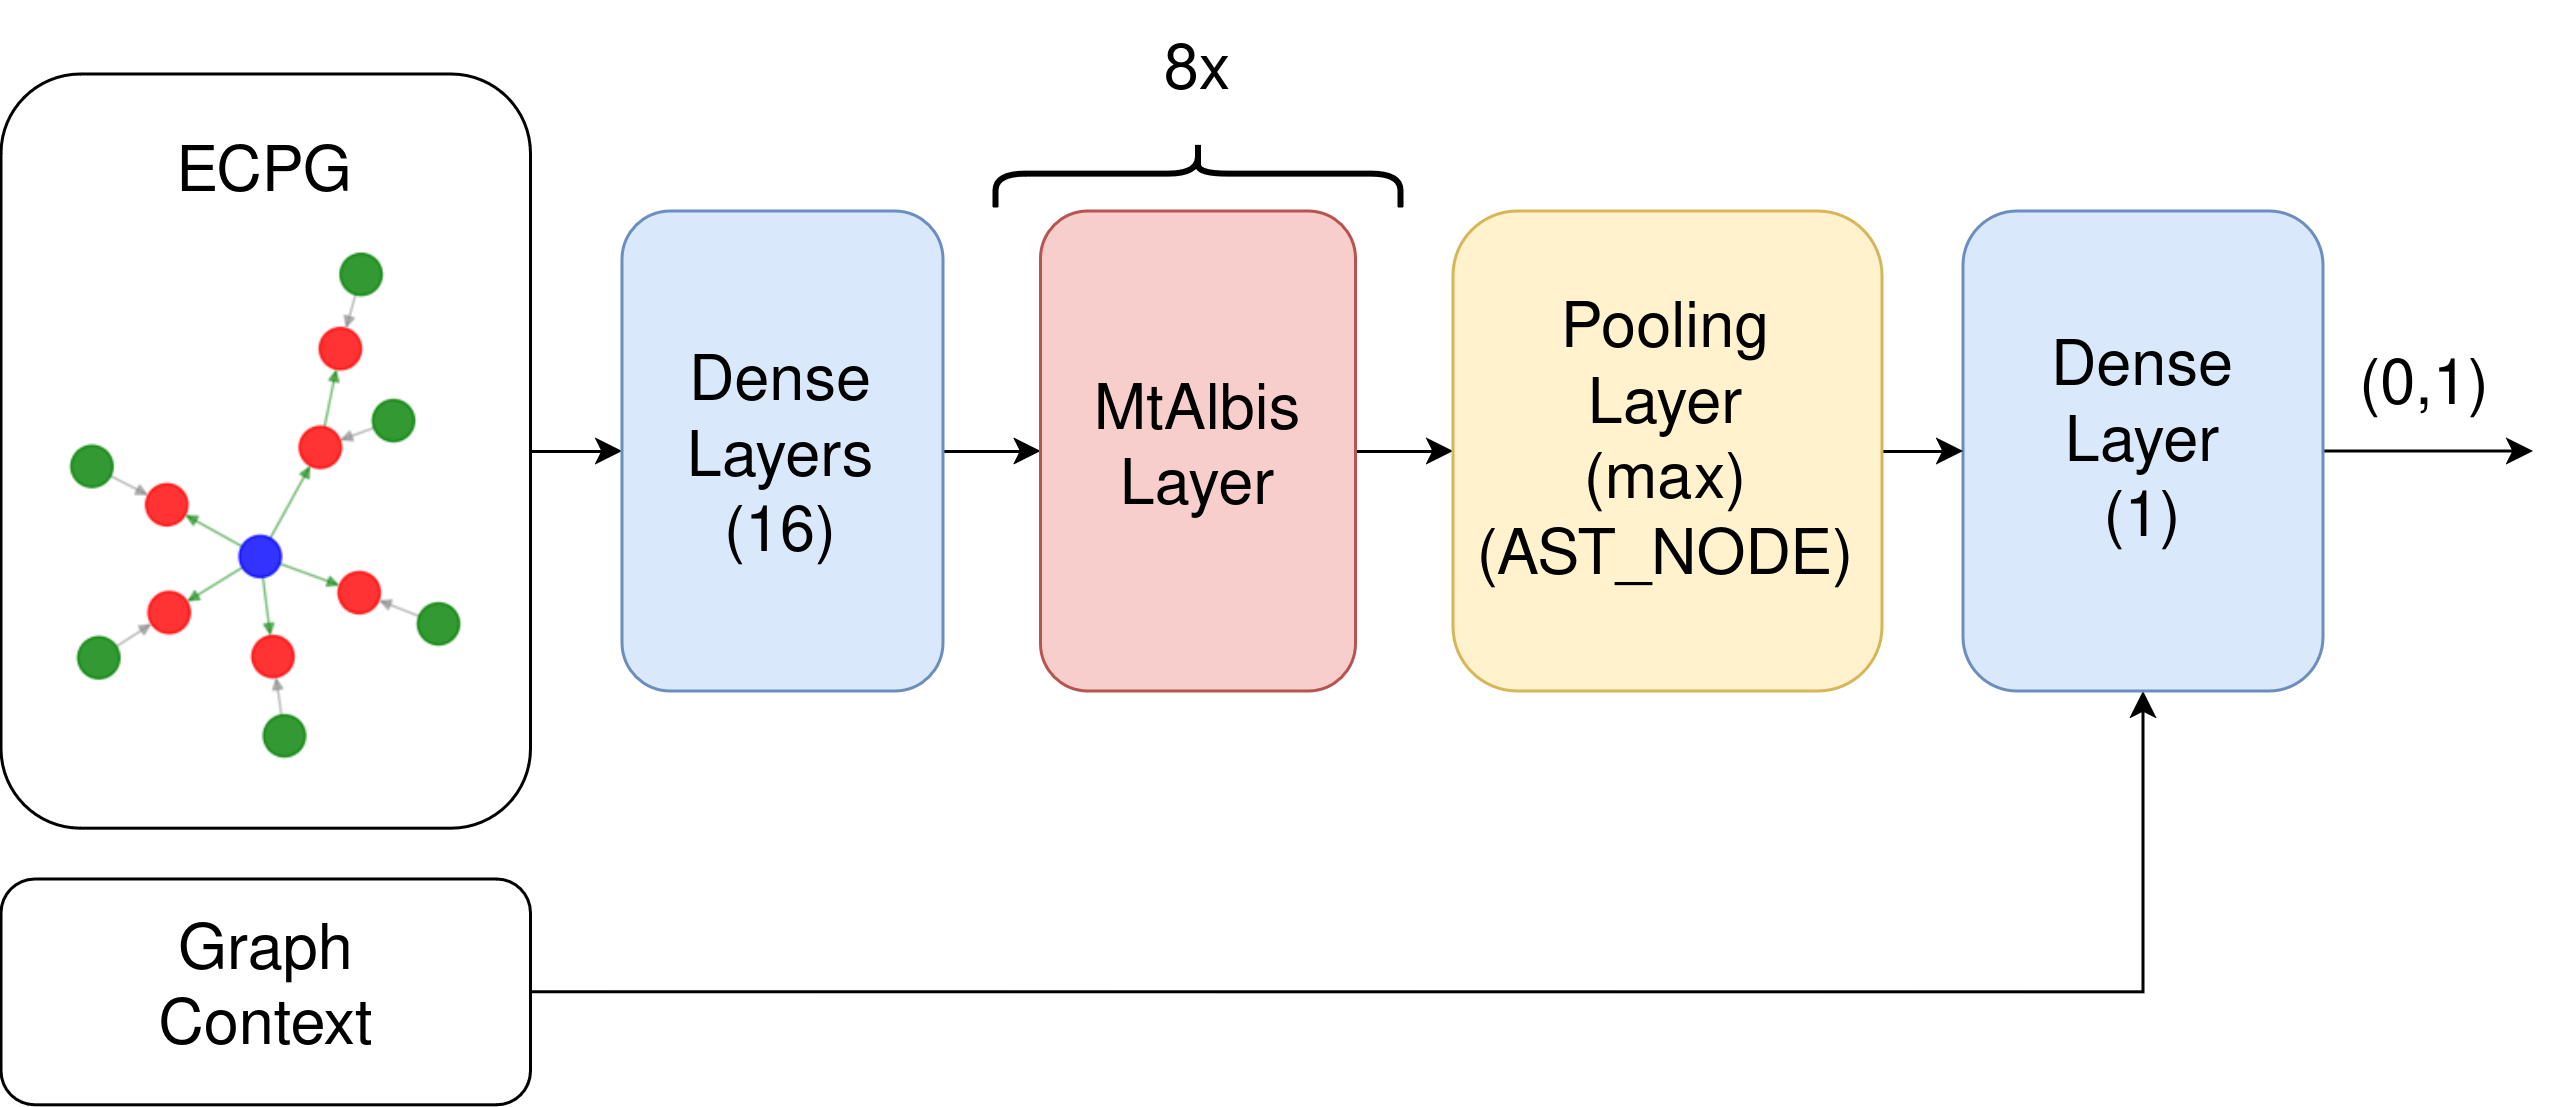
\includegraphics[width=0.9\textwidth]{figures/base-model.png}
    \caption{The figure shows the architecture of the base model (\texttt{Model 1}), which forms the basis for all other models developed in this thesis.}
    \label{figure:base-model}
\end{figure}

The architecture of the base model is shown in Figure~\ref{figure:base-model}. The layer initializing hidden states is of type \texttt{Dense(16)} (i.e., a densely-connected neural network layer with 16 outputs) with an activation function \texttt{relu}, for each node set. This is followed by 8 GNN layers of the type \texttt{MtAlbis}. Initial parameters were chosen primarily based on~\cite{tfgnn-mtalbis} and examples in the TFGNN repository\footnote{\textbf{TFGNN}'s repository: \url{https://github.com/tensorflow/gnn}.}. Parameters such as \texttt{units} and \texttt{message\_dim} were selected considering the batch size and GPU memory size. Some initial parameters were chosen randomly and for parameters not mentioned here, default values were retained. All (except for the last) \texttt{MtAlbis} layers share the same parameters, which are:
\begin{itemize}
    \item \texttt{units=16} -- size of the hidden states.
    \item \texttt{message\_dim=16} -- size of the messages on the edges.
    \item \texttt{receiver\_tag=tfgnn.TARGET} -- specifies the direction of message passing, here it is along the direction of the edges (\texttt{tfgnn.SOURCE} would be in the opposite direction).
    \item \texttt{node\_set\_names=None} -- updates nodes of all node set types. For the last layer, the value is set to \texttt{AST\_NODE} in order to modify only nodes from the \texttt{AST\_NODE} node set from which the following pooling layer reads. Hidden states of other node sets are discarded by the pooling layer, making it unnecessary to update their values in the last round of message passing.
    \item \texttt{state\_dropout\_rate=0.1} -- the dropout rate applied to the pooled and combined messages from all edges.
    \item \texttt{simple\_conv\_reduce\_type='mean|sum'} -- the type of message aggregation.
    \item \texttt{next\_state\_type=residual} -- can be set to \texttt{dense} or \texttt{residual}, where \texttt{residual} adds a residual connection from the old to the new node state.
\end{itemize}

Following the \texttt{MtAlbis} layers is a \texttt{Pool} layer of type \texttt{max}, which reads hidden states only from nodes of the \texttt{AST\_NODE} node set. Here, for example, it could read from the root of the AST tree, where information would accumulate when changing the orientation of the \texttt{AST} edges (as mentioned in Section~\ref{feature-engineering}), but this would require the tree depth to be equal to or less than the number of GNN layers so that information from leaf nodes could reach the root. Since the depth varies and ECPGs are not just trees, it utilizes all \texttt{AST\_NODE} nodes whose information is eventually aggregated using the \texttt{Pool} layer.

The context features, along with the output of the \texttt{Pool} layer, are inputs to the \texttt{Dense(1)} layer with the \textit{sigmoid activation function}, which transforms the values into the range $(0,1)$. The base model uses the \texttt{Adam} \textit{optimizer} with a learning rate of \texttt{0.000002}. The loss function used is \texttt{BinaryCrossentropy}. The model is trained in batches of size \texttt{11} (limited due to GPU memory) over \texttt{300} epochs, where the number of steps per epoch is the dataset size divided by batch size. The model employs \texttt{EarlyStopping} with \texttt{patience} set at \texttt{20} (thus, the models are not trained for 300 epochs but only for tens of epochs, see Section~\ref{hyperparameter-tuning}). The base model is trained separately on each project from D2A -- this represents a form of \textit{3-fold validation}.

Although the architecture is trained for binary classification, the goal of the models is ranking, not classification. Therefore, it does not make sense to monitor separate metrics such as \textit{precision}, \textit{recall}, or \textit{accuracy} in this case, since these are designed specifically for classification. These metrics are also not suitable for unbalanced data. The metric that appropriately reflects ranking and can be used for unbalanced data is the Area Under the Receiver Operating Characteristic Curve (AUROCC). The ROCC~\cite{aurocc} plots the \textit{True Positive Rate} (i.e., recall) on the Y-axis and the \textit{False Positive Rate} on the X-axis for each classification threshold (previously mentioned metrics use only a single threshold), thereby clearly describing the ranking ability of the model. The True Positive Rate is defined as (here true positives and false positives relate to the model, not to the results of Infer):
\begin{equation*}
True\:Positive\:Rate\:(TPR) = \frac{True\:Positives\:(TP)}{True\:Positives\:(TP) + False\:Negatives\:(FN)}
\end{equation*}
The False Positive Rate is then defined as:
\begin{equation*}
False\:Positive\:Rate\:(FPR) = \frac{False\:Positives\:(FP)}{False\:Positives\:(FP) + True\:Negatives\:(TN)}
\end{equation*}

AUROCC for a random model is 0.5 (indicated by a dashed line in all subsequent figures, see Figure~\ref{figure:auc-combined}) and for a perfect model is 1 (a model that can perfectly separate the classes). For the reasons mentioned above, AUROCC on validation data is monitored for early stopping in all trained models -- the models are thus trained to achieve the highest possible AUROCC.

\section{Hyperparameters Tuning}
\label{hyperparameter-tuning}
After the base model is created, it is necessary to tune its hyperparameters to adapt it to the specific task -- in this case, the ranking of reports from Infer. If, even after tuning the hyperparameters, the architecture does not yield satisfactory results, a different architecture is typically tried. As will be evident from the results below, the architecture of the base model achieved very good results during the hyperparameter tuning process. Therefore, there was an effort to optimally tune this architecture. Due to limited computing resources, it was not possible to use automated hyperparameter tuning, which typically involves training many models with different settings. Thus, a manual approach had to be used, which requires fewer computing resources compared to automatic tuning but relies on experience and knowledge in the field.

A total of 14 models were trained, the results on validation data and their number of parameters are in Table~\ref{tab:tuning}. The models are trained and tested, due to limited computing resources, only on the smallest projects -- httpd, libtiff, and nginx. The AUROCC of each model is either the average validation AUROCC across the individual projects or the validation AUROCC on a set of validation data composed of all the tested projects, as detailed below.

The following description includes a list of changes for each model compared to the previous model:
\begin{enumerate}
    \item \texttt{Model 1} -- base model, described in Section~\ref{base-model}.
    \item \texttt{Model 2} -- increased network complexity -- hidden state size increased to 18, an additional \texttt{MtAlbis} layer added, a \texttt{Dense(4)} added for context features, and a \texttt{Dense(8)} layer added before the final \texttt{Dense(1)} layer. The increase in complexity required reducing the batch size to 6. Also, the state dropout was increased to 0.15.
    \item \texttt{Model 3} -- reduced network complexity -- decreased the size of hidden states to 12 but increased the batch size to 10.
    \item \texttt{Model 4} -- reducing complexity led to much worse results, so complexity was further increased -- hidden state size increased to 20 at the cost of removing one \texttt{MtAlbis} layer and reducing the batch size to 6. A \texttt{Dropout(0.15)} layer was also added right after the \texttt{Pool} layer. The learning rate was decreased to 0.000001.
    \item \texttt{Model 5} -- added one \texttt{MtAlbis} layer (total of 9) at the cost of reducing the size of hidden states to 18.
    \item \texttt{Model 6} -- instead of training 3 models for each project, \texttt{Model 6} (and all subsequent models) is trained on all 3 projects at once (combining their training and validation sets). The learning rate was substantially increased to \texttt{0.0001}, and the \texttt{Dropout} layer was removed from the GNN head.
    \item \texttt{Model 7} -- increased state dropout to 0.2, tried only \texttt{mean} for \texttt{simple\_conv\_reduce}, and switched to \texttt{dense} for \texttt{next\_state\_type}.
    \item \texttt{Model 8} -- since \texttt{Model 7} experienced a significant drop in AUROCC, \texttt{Model 6} was restored. Only the state dropout was kept at 0.2 and an L2 regularization was added with a value of \texttt{0.00001} since the training AUROCC for \texttt{Model 6} was nearly 0.95 -- the model manages to learn on training data, now it needs to better generalize.
    \item \texttt{Model 9} -- set edge dropout (in \texttt{MtAlbis} layers) to 0.2.
    \item \texttt{Model 10} -- the edge dropout led to a significant deterioration, so it was set back to 0. However, the state dropout was increased to 0.25, and the learning rate was decreased to 0.00005.
    \item \texttt{Model 11} -- again tried the so-far best \texttt{Model 8} but in a bi-directional mode -- the direction of message passing in the \texttt{MtAlbis} layers is alternated using the \texttt{receiver\_tag} parameter (see Section~\ref{base-model}).
    \item \texttt{Model 12} -- again tried \texttt{Model 8} and utilized edge features -- \texttt{ARGUMENT\_INDEX} (until now all edge features were ignored).
    \item \texttt{Model 13} -- again tried \texttt{Model 8} but with \textit{attention} -- trainable message aggregation in \texttt{MtAlbis} layers. Used type \texttt{gat\_v2} with 3 attention heads (4 are default, but the size of the hidden state -- 18 -- must be divisible by the number of attention heads).
    \item \texttt{Model 14} -- slightly increased the state dropout to 0.22.
\end{enumerate}

The models have only been briefly described. Their source files can be found in the GitHub repository in commits labeled as, for example, \texttt{Model 8 - AUC 0.818}\footnote{Source code of \texttt{Model 8}: \url{https://github.com/TomasBeranek/but-masters-thesis/blob/fdcaa8e5f896d50c9b55a616cea84d56a058d45f/model/src/mixed_nodes_model.py}.} (the best-performing model). However, these historical versions of the training script (described in Section~\ref{implementation-training}) were in the development stage and should only serve as a reference for the definition of the model architectures.

From Table~\ref{tab:tuning}, it is evident that the best performing models are \texttt{Model 8}, \texttt{Model 13}, and \texttt{Model 10}, respectively. All these models are very small -- with less than 140 thousand parameters (which is about \textasciitilde500KB on disk) -- yet they achieve very good results. These models were trained (hardware specifications used are in Chapter~\ref{implementation}) for 69 epochs (\textasciitilde460s per epoch), 7 epochs (\textasciitilde1,350s per epoch), and 73 epochs (\textasciitilde450s per epoch), respectively.

\begin{table}
    \centering
    \caption{The table shows the results of hyperparameter tuning and the size of each model. Validation data from httpd, libtiff, and nginx projects were used for the evaluation.}
    \vskip6pt
	\begin{tabular}{
        !{\vrule width 1pt}l!{\vrule width 1pt}c|c!{\vrule width 1pt}}
        \noalign{\hrule height 1pt}
        Model & Parameters & AUROCC \\
        \noalign{\hrule height 1pt}
        Model 1& 96,515  & 0.630 \\
        Model 2& 137,499  & 0.668 \\
        Model 3& 61,941 & 0.557 \\
        Model 4& 150,093 & 0.607 \\
        Model 5& 137,499 & 0.598 \\
        Model 6& 137,499  & 0.787 \\
        Model 7& 106,071  & 0.632 \\
        \rowcolor{green1} Model 8& 137,499  & 0.818 \\
        Model 9& 137,499  & 0.775 \\
        \rowcolor{green3} Model 10& 137,499 & 0.793 \\
        Model 11& 140,523  & 0.786 \\
        Model 12& 140,451  & 0.788 \\
        \rowcolor{green2} Model 13& 109,563  & 0.816 \\
        Model 14& 109,563  & 0.746 \\
        \noalign{\hrule height 1pt}
    \end{tabular}
    \label{tab:tuning}
\end{table}


\section{Models Comparison}
\label{model-comparison}
As previously mentioned, this thesis compares with the models developed in~\cite{D2A-zheng2021d2a, pujar2024analyzing} which also focus on reducing false positives reported by Infer. For this comparison, the three best-performing models on the validation data, specifically \texttt{Model 8}, \texttt{Model 10}, and \texttt{Model 13}, were selected based on Table~\ref{tab:tuning}. Additionally, a \texttt{3-soft-vote} model was created, which ranks based on a \textit{soft score} -- the sum of the scores from the three top-performing models. Moreover, a \texttt{6-soft-vote} model comprising the six top-performing models (\texttt{Model 6}, \texttt{8}, \texttt{10}, \texttt{11}, \texttt{12}, and \texttt{13}) was also created. It is important to note that the models are not compared on identical test sets as the Graph D2A contains fewer samples than the original D2A dataset due to:
\begin{enumerate}
    \item Support for only certain error types (see Section~\ref{bitcode-generation}). The number of unsupported samples is \textasciitilde1.6~\% of the total D2A samples, thus minimally influencing the results.
    \item The inability to generate ECPG from some D2A samples. These cases are significantly more frequent and could more substantially impact the results. Their quantity varies depending on the project, ranging from 3~\% to 23~\% for tested projects (see Table~\ref{tab:implementation-d2a}).
\end{enumerate}

Table~\ref{tab:comparison} presents a comparison of the \texttt{Model 8}, \texttt{Model 10}, \texttt{Model 13}, \texttt{3-soft-vote}, and \texttt{6-soft-vote} developed in this thesis with the existing \texttt{vote}, \texttt{c-bert}, and \texttt{vote-new} models from~\cite{D2A-zheng2021d2a, pujar2024analyzing}. The models are compared based on AUROCC on the test data, which is the only common metric across all models. The comparison is only shown for the projects httpd, libtiff, and nginx due to limited computational resources. The \texttt{vote}, \texttt{c-bert}, and \texttt{vote-new} models are trained on training and validation data, whereas the models developed in this thesis are trained only on training data with validation data used for early stopping.

\begin{table}
    \centering
    \caption{A comparison of the existing models \texttt{vote}, \texttt{c-bert}, and \texttt{vote-new} with the models developed in this thesis. The comparison criterion is AUROCC on test data.}
    \vskip6pt
	\begin{tabular}{
        !{\vrule width 1pt}l!{\vrule width 1pt}c|c|c!{\vrule width 1pt}}
        \noalign{\hrule height 1pt}
        \textbf{Model} & \textbf{httpd} & \textbf{libtiff} & \textbf{nginx} \\
        \noalign{\hrule height 1pt}
        vote & 0.77 & 0.89 & 0.77 \\ \hline
        c-bert & \cellcolor{green3} 0.82 & 0.94 & 0.89 \\ \hline
        vote-new & \cellcolor{green1} 0.90 & \cellcolor{green1} 0.98 & \cellcolor{green3}0.93 \\ \hline
        \noalign{\hrule height 1pt}
        Model 8 & 0.80 &  \cellcolor{green3} 0.95 & \cellcolor{green2}0.94 \\ \hline
        Model 10 & 0.79 & 0.91  & 0.91 \\ \hline
        Model 13 & 0.74 &  0.87 & 0.83 \\ \hline
        3-soft-vote & 0.80 &  \cellcolor{green2} 0.96 & \cellcolor{green1}0.95 \\ \hline
        6-soft-vote & \cellcolor{green2} 0.83 & \cellcolor{green2} 0.96 \cellcolor{green2} & \cellcolor{green2} 0.94 \\ \hline
        \noalign{\hrule height 1pt}
    \end{tabular}
    \label{tab:comparison}
\end{table}

From Table~\ref{tab:comparison}, it is evident that the developed GNN models can match or even surpass the state-of-the-art models, especially for nginx. However, the results for httpd are lower, likely due to a lack of data. As indicated in Table~\ref{tab:tuning}, models using a combined training set (\texttt{Model 6} and above) achieve significantly better results. It is possible that compared to existing models, these GNNs require more training data. The httpd project has the fewest samples in the original D2A dataset, and an additional \textasciitilde22~\% of samples were removed when generating Graph D2A from httpd, which greatly complicates learning.

However, models can also be compared from other perspectives, such as their size, which relates to the inference speed. All existing solutions are closed source, making it impossible to determine their sizes. Similarly, it is not possible to verify their results, experiment with the models, or use them. Hence, the models developed in this thesis are a promising open source alternative.

Specific ROC curves for the developed models on the combined test sets can be seen in Figure~\ref{figure:auc-combined}. ROC curves for individual projects are provided in the appendices in Figure~\ref{figure:auc-httpd} (httpd), Figure~\ref{figure:auc-libtiff} (libtiff), and Figure~\ref{figure:auc-nginx} (nginx).

\begin{figure}[ht]
	\centering
	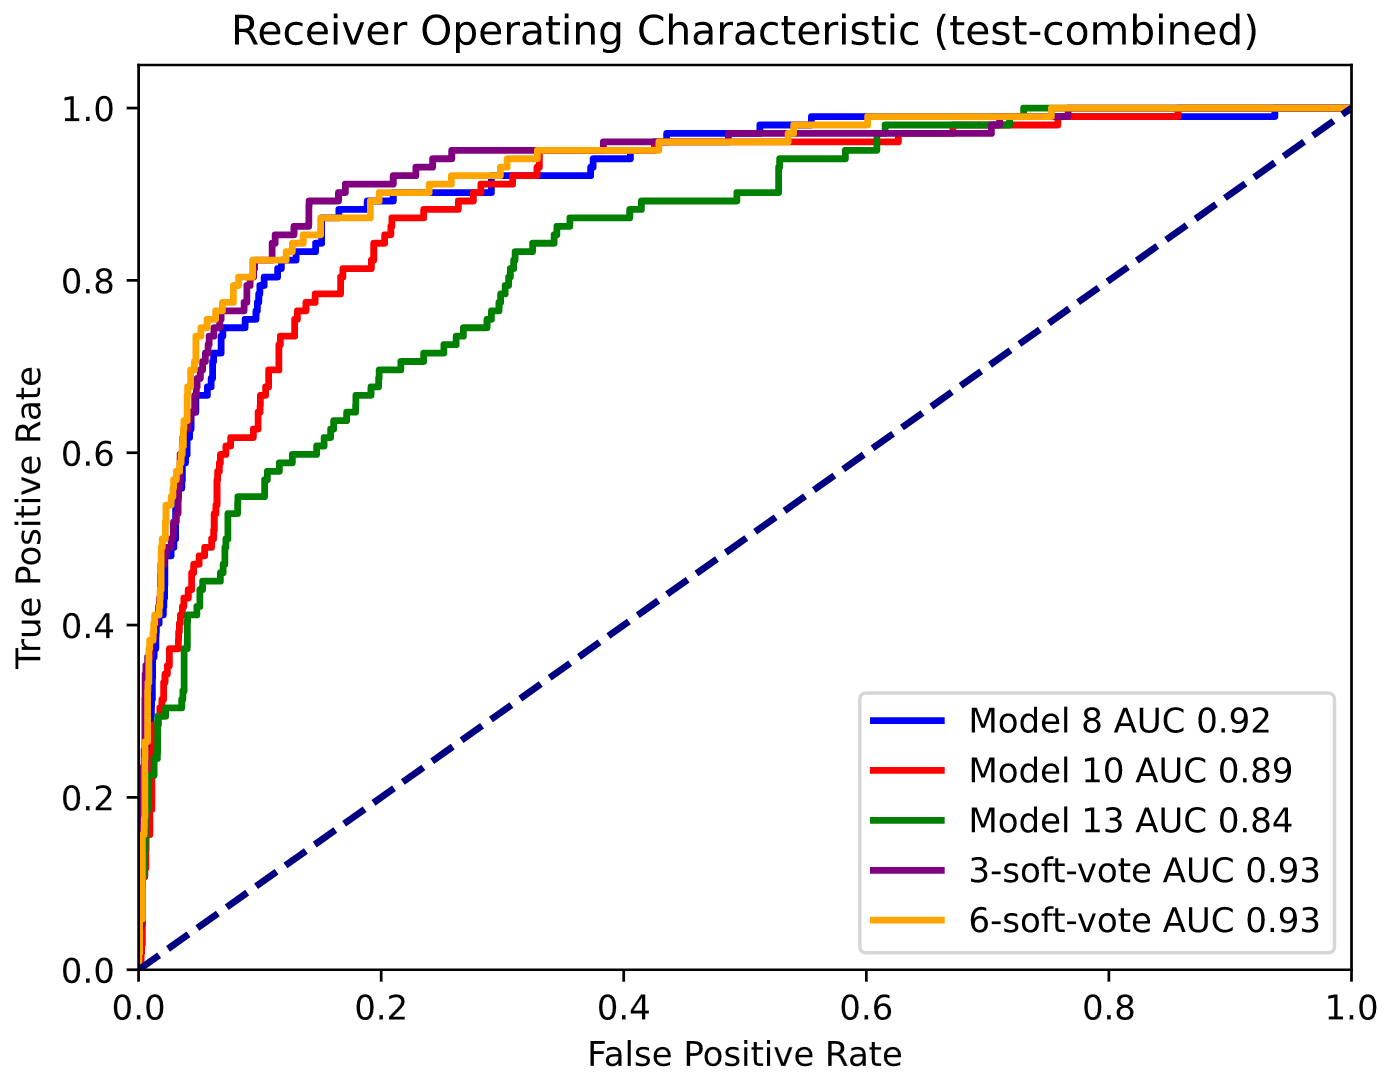
\includegraphics[width=0.75\textwidth]{figures/auc-combined.png}
	\caption{The figure shows the ROC curves for the top-performing models developed in this thesis, evaluated on a combined test set from the httpd, libtiff, and nginx projects.}
	\label{figure:auc-combined}
\end{figure}

The intended use case for these models is to rank Infer reports by likelihood of being a~real error. Developers would then typically check only the most promising reports -- for example, the top 5~\% (the same value was chosen in~\cite{pujar2024analyzing}). Consider now the best-performing model (on average), \texttt{6-soft-vote}, which is deployed on the test data of the libtiff project. The percentage of real errors (equivalent to $precision * 100$) in the libtiff project test data in Graph D2A is \textasciitilde4.7~\% (see Table~\ref{tab:implementation-d2a}). This number remains unchanged (on average) if a~random 5~\% of samples are checked -- equivalent to ranking by a random model. However, if the top 5~\% of samples according to the \texttt{6-soft-vote} model are selected, the amount of true positives increases to \textasciitilde57.1~\%. In terms of the number of samples -- in unsorted reports, there will be on average 2.3 real errors for every 49 checked reports. In the sorted reports, 28 real errors will be found for the same number of checked reports, which is more than 13 times as many.

Graphs showing precision values for different percentages of top samples and for top-performing models are presented in Figure~\ref{figure:topn-combined} (combined data from all projects), Figure~\ref{figure:topn-httpd} (httpd), Figure~\ref{figure:topn-libtiff} (libtiff), and Figure~\ref{figure:topn-nginx} (nginx). This metric becomes more sensitive as fewer top samples are considered.


\section{Comparison with ChatGPT}
\label{comparison-chatgpt}
In recent years, Large Language Models (LLMs) such as ChatGPT have become increasingly recognized by both professionals and the general public. ChatGPT can respond to textual inputs (and in version 4, even, e.g., image inputs) with textual outputs (again in version 4, even, e.g.,  image outputs). The introduction of ChatGPT~\cite{chatgpt} demonstrates the model's capabilities to search for and correct errors in code. The ability of ChatGPT (especially version 4) to handle programming tasks compared to other LLMs is discussed in~\cite{coello2024effectiveness}, where ChatGPT4 is shown to be particularly effective. These results raise the question of how ChatGPT might perform in reducing false reports.

For the experiment, the \texttt{6-soft-model}, which on average achieved the best results in Section~\ref{model-comparison}, was used. Ten true positives and ten false positives were randomly selected from the test set of the libtiff project. These samples, in their original JSON format (without class information), were submitted to a modified version of ChatGPT4 that could interpret code and search the internet, with the following instructions:
\begin{lstlisting}[language=bash, xleftmargin=2em]
Behave like a binary classification model. You will receive a sample 
from the D2A dataset, containing reports from Meta Infer static 
analyzer. Your goal is to output a number in the range <0,1>. The 
higher the number, the more certain you are that the report from Infer
is true. Individual samples contain the report itself, the location of 
the error, codes of functions related to the error, and other useful 
information.
\end{lstlisting}

From Figure~\ref{figure:auc-chatgpt}, which displays the ROC curves for the scores from \texttt{6-soft-vote} and from ChatGPT version 4, it is apparent that ChatGPT4 exhibits random behavior in terms of ranking these selected samples. In contrast, \texttt{6-soft-vote} achieves a perfect score -- distinguishing between the classes perfectly. When comparing the models in terms of their size, \texttt{6-soft-vote} again prevails with only 800 thousand parameters (comprising 6 sub-models), while ChatGPT4 has approximately 1.76 trillion parameters~\cite{chatgpt-params}. However, it is important to note that ChatGPT is a general-purpose model and not a classifier specifically designed for ranking reports from static analysis.

\begin{figure}[t]
	\centering
	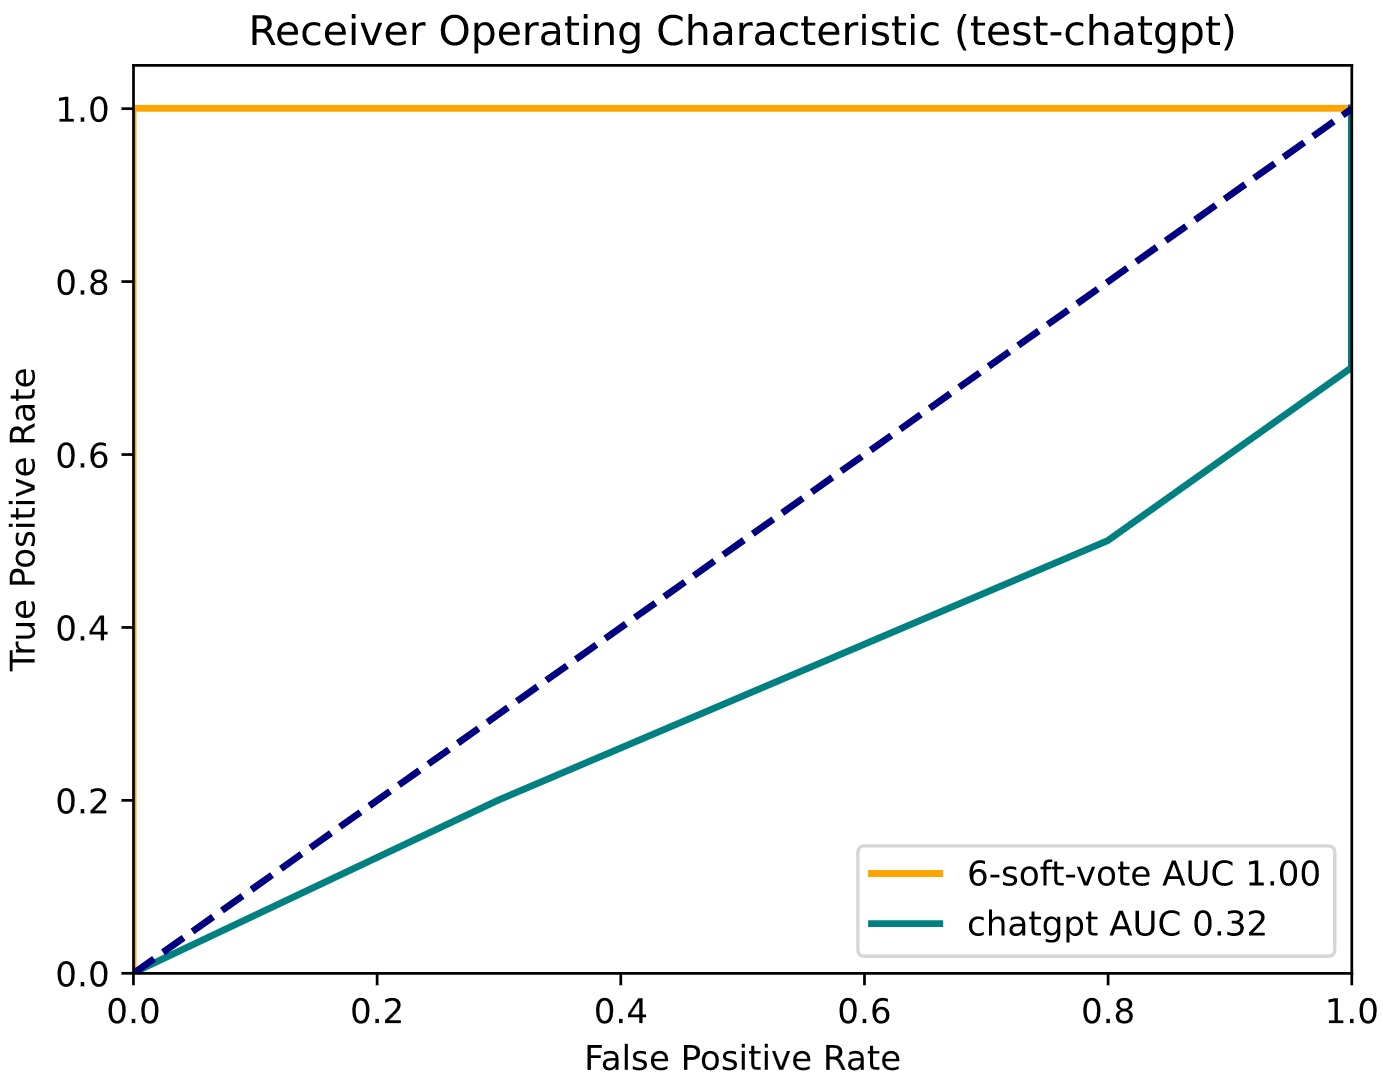
\includegraphics[width=0.75\textwidth]{figures/auc-chatgpt.png}
	\caption{The figure shows ROC curves comparing \texttt{6-soft-vote} and ChatGPT4, on a randomly selected (with balanced classes) 20 samples from the test data of the libtiff project.}
	\label{figure:auc-chatgpt}
\end{figure}

\section{Cross-analysis}
\label{cross-analysis}
The ultimate goal of all models in the field of static analysis report filtering/ranking, based on the likelihood of being true positive, is to function on cross-analysis. Existing models \texttt{vote}, \texttt{c-bert}, and \texttt{vote-new} from~\cite{D2A-zheng2021d2a, pujar2024analyzing} are designed only for self-analysis -- the model is trained and tested on the same project. However, the self-analysis is also useful in practice, especially for large projects with extensive git histories that can be used to train models. 

A primary objective of feature engineering in Section~\ref{feature-engineering} was to eliminate information that could lead the models to overfit to a specific project. To test cross-analysis capabilities, the top performing models were tested on the test data of the libav project. The results in Figure~\ref{figure:auc-libav} indicate that the models, on average, exhibit random behavior. The developed models, like all existing ones, thus fail to function on cross-analysis, which represents a~significant challenge in this research field.

\begin{figure}[t]
	\centering
	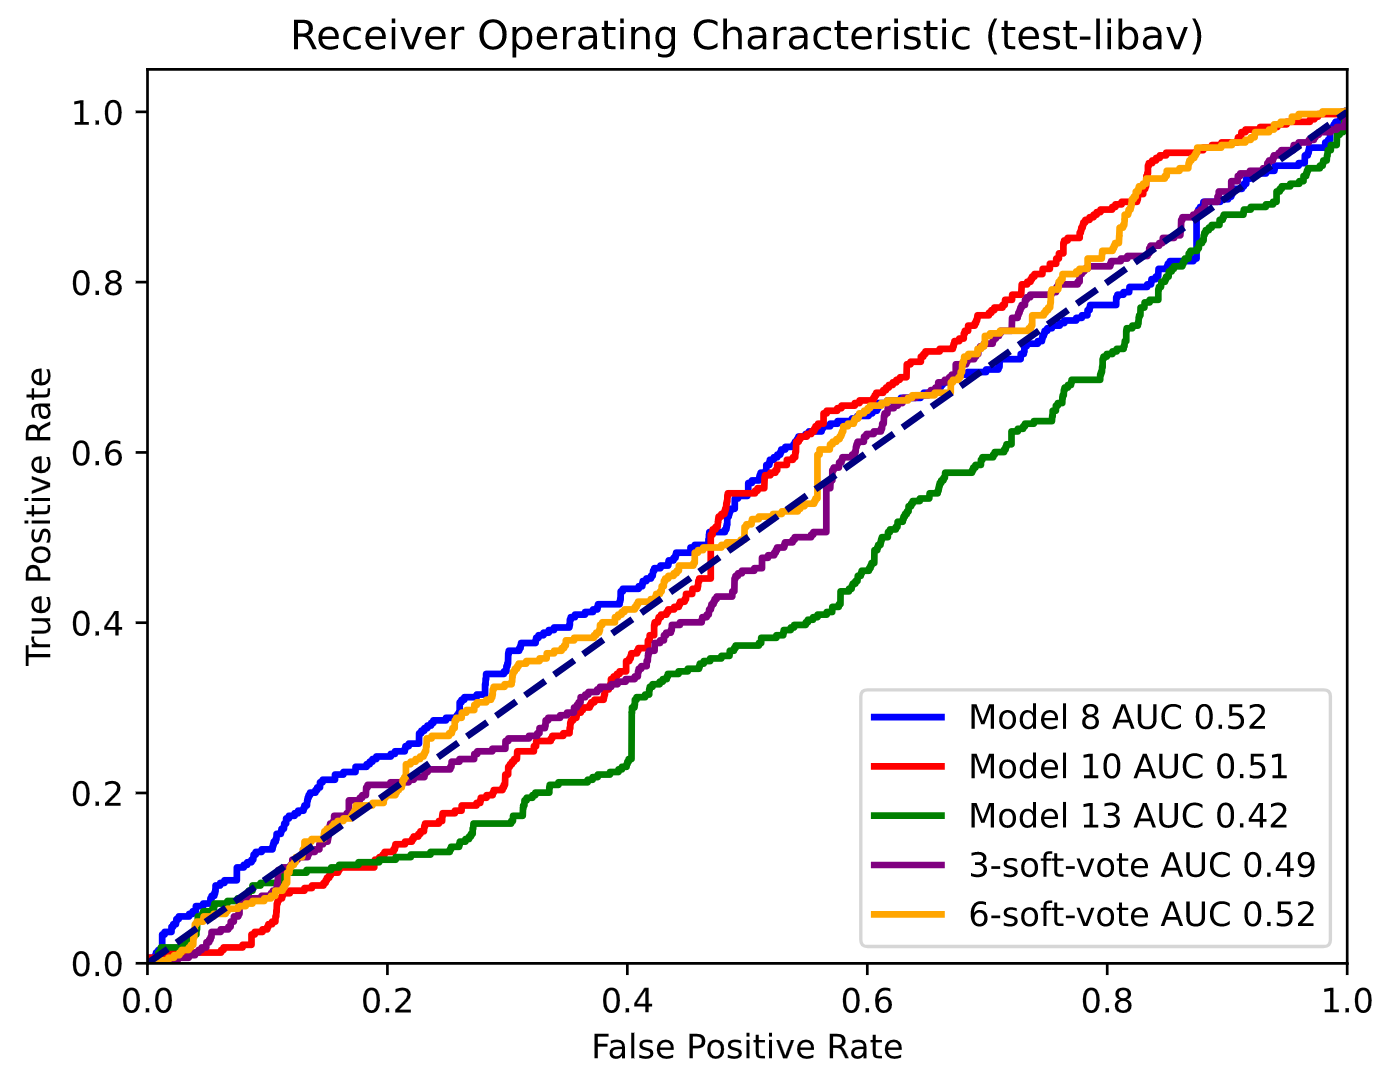
\includegraphics[width=0.75\textwidth]{figures/auc-libav.png}
	\caption{The figure shows ROC curves for the top performing models developed in this thesis in cross-analysis mode. The models were trained on the httpd, libtiff, and nginx projects and tested on the test data of the libav project.}
	\label{figure:auc-libav}
\end{figure}

\section{Summary and Future Work}
\label{summary}
From the experiments in this chapter, it is evident that GNNs, and specifically the models developed in this thesis, are suitable for ranking reports from the Meta Infer static analyzer. The created models were able to match best existing solutions in this area that we are aware of, which were developed by strong industrial team from IBM. In the case of the nginx project, the existing models were even surpassed. However, results on the httpd project were weaker, which may be due to a lack of data for the httpd project, which is not only the smallest project in terms of the number of samples in the D2A dataset but also experienced high sample losses during the generation of Graph D2A. Nonetheless, we believe that these results demonstrate that the developed models are a promising open-source alternative to existing solutions, which are unfortunately all closed source.

The best-performing model, \texttt{6-soft-vote}, was also compared with the LLM model ChatGPT version 4. The model developed in this thesis proved superior with a perfect score, in contrast to ChatGPT4, which was unable to differentiate between false and real reports.

The models were also tested on a cross-analysis. None of the models were able to correctly distinguish false reports from real ones. Cross-analysis thus emerges as an unexpectedly challenging problem in this research area as no existing model that we are aware of functions effectively on cross-analysis either.

Future work should focus on testing self-analysis on all projects in the D2A dataset, which, however, requires training on a large number of samples and thus needs significant computational resources. Considering the results of experiments on the httpd project, it would be necessary to focus on improving the training pipeline to avoid such high sample losses. Specifically, it would be beneficial to increase the timeout for the LLVM Slicer tool and to focus on improving the success rate of LLVM bitcode extraction. Particularly, it should focus on the minority class -- true positives (not just for httpd), which are naturally very scarce.

Various ways of future improvements have already been mentioned in previous chapters. Considering the results of the models on cross-analysis, it would be necessary to focus especially on adjusting feature engineering -- more information that allows models to overfit on individual projects should be discarded. Additionally, refining the extraction of slicing criteria could help future graphs to contain less \textit{noise} (i.e., redundant information).

There is also a plan to deploy the developed models as part of the csmock tool~\cite{CsmockAVM,CsmockFLOCK}, which allows the automatic running of various analyzers on SRPM packages. A plugin for the csmock tool that adds support for static analysis by Meta Infer was created in the author's bachelor's thesis~\cite{bc}. It would simply involve supplementing this plugin with the developed models, which would rank the results of Infer.


\chapter{Conclusion}
\label{conclusion}
This thesis aimed to develop a machine learning-based system for ranking reports from the Meta Infer static analyzer based on their likelihood of being real error. Graph Neural Networks (GNNs) were selected due to their suitability for modeling various source code properties. The D2A dataset from IBM, which contains labeled Infer reports, was used for training. This dataset required conversion from a textual to a graphical format. To achieve this, a training pipeline was developed to produce Graph D2A -- a graphical representation of D2A. This pipeline improves existing graph generation techniques by considering conditional compilation. The raw format of graphs in Graph D2A necessitated the design of a feature engineering process that optimizes and transforms these graphs into Extended Code Property Graphs (ECPGs), which enrich commonly used Code Property Graphs by including Call Graphs, data types, and other information.

Experimental results with GNN models trained on projects httpd (AUROCC 0.83), libtiff (AUROCC 0.96), and nginx (AUROCC 0.94) show that the developed models are competitive with existing state-of-the-art solutions created by strong industrial teams. The models even reached state-of-the-art results on the nginx project although they performed less well on the httpd project, likely due to a low number of samples. Nonetheless, these experiments show that the developed models are a promising open-source alternative since all existing solutions are closed-source. The models were also tested using cross-analysis, which unfortunately did not yield useful results. Cross-analysis remains a significant challenge as none of the existing models compared in this thesis function effectively in this mode either.

In this thesis, an inference pipeline was also developed for the automatic Infer analysis, construction of ECPGs, and model inference on real-world C (and subset of C++) software. Even if cross-analysis does not work, the inference pipeline could be utilized in the future for inference on the projects on which the models were trained.

Future work should focus on evaluating and fine-tuning the developed models on larger projects from the D2A dataset. Based on the experiment results from the httpd project, the training pipeline should be improved to minimize the loss of samples during transformation. Specifically, increasing the timeout for the LLVM Slicer tool and focusing on generating LLVM bitcode, especially for the minority class -- real errors. There are also plans to deploy the developed models in the csmock tool, which automates analyses on SRPM packages.

Preliminary results of this thesis were presented at the Excel@FIT'24 conference, where it received an award from the expert panel.
\vspace{-1cm}
  \else
    % Tento soubor nahraďte vlastním souborem s obsahem práce.
%=========================================================================
% Autoři: Michal Bidlo, Bohuslav Křena, Jaroslav Dytrych, Petr Veigend a Adam Herout 2019

% Pro kompilaci po částech (viz projekt.tex), nutno odkomentovat a upravit
%\documentclass[../projekt.tex]{subfiles}
%\begin{document}

\chapter{Úvod}

Tento text slouží jako ukázkový obsah šablony a současně rekapituluje nejdůležitější informace z předpisů a poskytuje další užitečné informace, které budete potřebovat pro tvorbu technické zprávy ke svojí práci. Než se šablonou budete dále pracovat, je třeba vědět, jak ji správně použít. To je stručně uvedeno v~příloze \ref{jak}.

I když některým studentům pro napsání dobré diplomové práce (bakalářská práce je také diplomová -- dostává se za ni diplom) stačí znát a dodržovat oficiální formální požadavky uvedené ve směrnicích a typografické zásady, často je výhodné před započetím psaní zjistit, jaké jsou osvědčené postupy pro psaní odborného textu a jak si práci usnadnit. Někteří vedoucí svým studentům připravili popisy osvědčených postupů, které vedly k desítkám úspěšně obhájených prací. Výběr nejzajímavějších postupů, které měli autoři této šablony k~dispozici ve chvíli její tvorby, je v níže uvedených kapitolách. Má-li Váš vedoucí svoji stránku s doporučenými postupy, tyto kapitoly můžete vynechat a řídit se pokyny svého vedoucího. Pokud takovou stránku nemá, může být přečtení níže uvedeného textu vhodnou přípravou na konzultaci o plánované struktuře a náplni textu práce.

Diplomová práce je rozsáhlé dílo a tomu odpovídá i technická zpráva. Ne každý je schopen si sednout a jednoduše ji napsat. Je třeba vědět, kde začít a jak postupovat. Jedním z možných přístupů je začít psaním klíčových slov a abstraktu, abyste si ujasnili, co je v~práci nejdůležitější. O tom pojednává kapitola \ref{abstrakt}.

Po sepsání abstraktu se lze pustit do psaní samotného textu technické zprávy. Typicky si nejprve připravíme základní strukturu práce, kterou pak budeme plnit textem. Kapitola \ref{struktura} se zabývá základními informacemi a radami pro psaní odborného textu, které Vám pomohou vyhnout se začátečnickým chybám, a stanovením nadpisů kapitol a přibližných rozsahů jednotlivých částí práce. V závěru kapitoly je pak uveden přístup, kterým si lze psaní technické zprávy značně usnadnit.

Diplomové práce v oblasti informačních technologií mají určitou typickou strukturu. Po~úvodu bude následovat kapitola či kapitoly zabývající se shrnutím současného stavu, který bude v následujících kapitolách zhodnocen a bude navrženo řešení, které bude implementováno a otestováno. V závěru pak budou výsledky vyhodnoceny a bude navržen budoucí vývoj. I když se názvy a rozsahy kapitol v různých pracích liší, vždy tam lze najít kapitoly odpovídající této struktuře. Kapitola \ref{kapitoly} se zabývá obsahy typických kapitol, které se v diplomových pracích z oblasti IT vyskytují. Většina studentů ve svojí práci pravděpodobně využije pouze určitou podmnožinu popsaných kapitol, která je pro jejich práci relevantní. Uvedené popisy a rady mohou pomoci jak s~rozhodnutím, zda danou kapitolu uvést, tak i~s~vnitřní strukturou a samotným obsahem kapitoly.

Za závěrečnou kapitolou práce vždy následuje seznam použité literatury. Citacemi, které tento seznam tvoří, a odkazy na ně se zabývá kapitola \ref{citace}. Byť to tak nezkušený student nemusí vnímat, je seznam použité literatury a odkazy na něj pro práci zcela zásadní. Hodnocení práce s literaturou a citací tvoří jednu z důležitých částí posudku oponenta a bude-li chybět jediná položka, může to vést k hodnocení stupněm F, následnému disciplinárnímu řízení za plagiátorství a k vyloučení z nedokončeného studia. Nesprávná práce se zdroji může mít i další důsledky -- v roce 2018 stála křesla dva členy české vlády. Proto prosím citacím věnujte odpovídající pozornost. 

Po dokončení textu je nutné zjistit, jaké požadavky jsou kladeny na vysokoškolskou kvalifikační práci na FIT VUT v~Brně, a dořešit případné nedostatky. Formální požadavky jsou uvedeny ve směrnicích a na webových stránkách, které jsou zmíněny v kapitole \ref{formality}. Tato kapitola obsahuje i požadované rozsahy jednotlivých typů prací a další vybrané informace z~předpisů a doporučení. V závěru kapitoly je uveden přehled nejčastějších chyb, se kterými se oponenti setkávají a kterým byste se měli vyhnout. Hodnocení formální úpravy práce je pak další z důležitých součástí posudku oponenta.

Po odstranění formálních nedostatků lze práci odevzdat. Před odevzdáním práce si můžete projít kontrolní seznam (tzv. \uv{checklist}) uvedený v příloze \ref{checklist}. Samotné odevzdání listinné i elektronické verze práce je pak popsáno v kapitole \ref{odevzdani}.

V závěrečné kapitole \ref{zaver} je pak uvedeno shrnutí toho, co se lze přečtením tohoto textu dozvědět, a to nejdůležitější, na co je třeba myslet před odevzdáním práce.


\chapter{Abstrakt}
\label{abstrakt}
Pod nadpisem Abstrakt je uvedeno shrnutí práce zabírající prostor maximálně 10 řádků. Z~dobrého abstraktu by mělo být i přes jeho malý rozsah patrné, jaký problém se řešil, jaký přístup k jeho řešení byl v práci použit a jakých výsledků bylo dosaženo. Účelem abstraktu je, aby potenciální čtenář práce již po přečtení abstraktu věděl, zda v práci najde to, co hledá \cite{fitWeb}. Zbytek této kapitoly byl převzat z blogu prof. Herouta \cite{Herout}.
\bigskip

\noindent Za prvé – na abstraktu záleží. Za druhé – není těžké ho napsat. Pojďme na to.

\subsection*{K čemu je abstrakt}
Abstrakt slouží k \bf vyhledávání\rm, společně s názvem dané vědecké práce a seznamem klíčových slov. Tyto části (snad s výjimkou názvu) nejsou přímo součástí textu a nečeká se, že někdo, kdo by zasedl ke čtení dané vědecké práce, bude číst je. To, že práci čte, znamená, že už se dostal za fázi čtení abstraktu. Abstrakt mu slouží ve chvíli, kdy se ještě rozhoduje, \bf zda vůbec \rm text číst.

Když někdo tam venku hledá odpověď na svůj problém, zadá knihovnici nebo dnes spíše vyhledávacímu serveru klíčová slova, která se jeho potíží dotýkají. Na základě shody těchto klíčových slov a klíčových slov uvedených autory dostane seznam názvů prací, které by mu mohly nabízet řešení. Dobře sestavený název práce badateli pomůže vytipovat takové texty, které by mohly mít vztah k jeho problému a mohl by se zajímat o jejich přečtení.

A tady právě přichází na scénu abstrakt. Badatel si čte abstrakt vytipovaných prací a~rozhoduje se, zda práci skutečně chce číst, nebo jestli se v tomto případě jeho filtr založený pouze na jednořádkovém nadpisu zmýlil.

V tuto chvíli obvykle ještě nemá stažené nějaké PDF s celým textem, natož aby měl v ruce vytištěný fascikl. Abstrakty jsou určeny k tomu, aby byly \bf mimo text\rm , aby ležely na serverech agregujících vědecké texty. Proto první pravidlo je, že abstrakt musí fungovat samostatně -- pokud obsahuje odkazy do literatury nebo se odvolává na text (\uv{Výkonnost metody je přehledně shrnuta na straně 51.}), nedělá badateli dobrou službu, což badatel ocení tím, že si o autoru nepomyslí nic hezkého, práci si nepřečte a autora neocituje.

\subsection*{Kdy a jak psát Abstrakt}
Může dávat smysl psát abstrakt na závěr celého psaní -- jako shrnutí a skutečné anotování sepsaného díla. Já jsem vyznavačem opačného přístupu -- abstrakt píšu na samém začátku. Když píšu vědecký článek, začínám sepsáním velkého počtu klíčových slov, jež se textu dotýkají. Bývá jich více, než potom uvedu jako ona charakteristická klíčová slova používaná k indexování. Ujasňuji si tím prostor, kde se článek pohybuje -- o čem je třeba hovořit, co je v textu podstatné, čeho se dotýká. Hned po ujasnění klíčových slov formuluji nadpis a~právě abstrakt. 

Považuji za mimořádně užitečné ujasnit si právě ony čtyři části abstraktu -- Jaký problém se řeší? Jaké řešení práce nabízí? Jaké jsou přesně výsledky? Jaký je jejich význam? Když je toto jasné, text se píše skoro sám. Pokud toto má být nejasné, jak u všech všudy je možné vůbec dát dohromady smysluplnou větu v samém textu?

\subsection*{Doporučená struktura abstraktu}
Abstrakt vědecké práce se může skládat ze čtyř částí a pak být opravdu užitečný. Každá část se bude skládat z nějakých dvou, tří vět, někdy postačí jedna.

V byznysu se vžil slovesný útvar \uv{elevator pitch} -- představení ve výtahu. Ne náhodou jeho struktura připomíná právě doporučovanou strukturu abstraktu. Opravdu, autor odborného textu má do abstraktu napsat právě to, co by říkal o své práci, kdyby na to měl nejvýše dvě minuty a nemohl použít žádných slajdů, obrázků, textu. O čem by tedy měl mluvit?

\paragraph{První část -- Jaký se řeší problém? Jaké je téma? Jaký je cíl textu?}
\begin{itemize}
  \item{Tato práce řeší.}
  \item{Cílem této práce je.}
  \item{Zaměřil jsem se na.}
\end{itemize}
Nepatří sem úvodní pohádky charakteristické pro špatný odborný sloh: \uv{Naše poslední pětiletka staví před nás nové a smělé cíle}, \uv{S rozvojem výpočetní techniky a zejména zobrazovacích zařízení je stále důležitější \ldots} Ty nepatří do dobrého textu nikam, ale do~abstraktu tím méně. Pokud dokážete vyjádřit účel svého textu v jedné větě o pár slovech, udělejte to a nepřidávejte nic navíc. Stručnější zde vždy znamená lepší.

\paragraph{Druhá část -- Jak je problém vyřešen? Cíl naplněn?}
\begin{itemize}
  \item{Zvolený problém jsem vyřešil pomocí toho a toho.}
  \item{V řešení bylo použito metody té, postupu toho a analýzy oné.}
  \item{Práce představuje algoritmus takový, který.}
  \item{Data jsem zpracovával pomocí těch a těchto nástrojů a provedl vyhodnocení takové.}
  \item{Podstatou našeho algoritmu je.}
\end{itemize}

Pokud je podstatou sepisovaného odborného textu nová metodologie (= \uv{jak něco dělat}), patří přesně sem její popis. Pokud se představované řešení skládá ze tří částí, pravděpodobně v této části abstraktu budou tři věty, z nichž každá se bude věnovat jedné části řešení. Dobrý abstrakt v této části bude upřímný a přesný -- nebude si schovávat \uv{odhalování svých tajemství} až do textu. Vágní formulace podstaty řešení v abstraktu obvykle znamená, že autoři buď neumí psát a nebo vlastně nemají o čem -- ani jedno není zrovna výzva ke stažení a čtení mnoha stran textu.

\paragraph{Třetí část -- Jaké jsou konkrétní výsledky? Jak dobře je problém vyřešen?}
\begin{itemize}
  \item{Podařilo se dosáhnout úspěšnosti 87,3\,\%.}
  \item{V práci jsme vytvořili systém, který.}
  \item{Vytvořené řešení poskytuje ty a ty možnosti.}
  \item{Provedeným výzkumem jsme zjistili, že.}
\end{itemize}

Není špatným zvykem uvést v této části konkrétní číslo -- \uv{existující metodu XY jsme zrychlili pětkrát}. Pokud přínos práce není možné shrnout do dvou nebo tří vět, někde je něco velmi špatně a celý text pravděpodobně nestojí za psaní.

\paragraph{Čtvrtá část -- Takže co? Čím je to užitečné vědě a čtenáři?}
\begin{itemize}
  \item{Přínosem této práce je.}
  \item{Hlavním zjištěním je.}
  \item{Hlavním výsledkem je.}
  \item{Na základě zjištěných údajů je možné.}
  \item{Výsledky této práce umožňují.}
\end{itemize}

Při psaní vědeckých článků já sám obvykle bojuji s podobností části třetí a čtvrté. Vskutku, obě hovoří o tom, co jsou výsledky a přínosy textu. Účelem třetí části je jmenovitě a konkrétně jmenovat dosažené výsledky, úkolem části čtvrté je interpretovat jejich význam. Asi ničemu nevadí, když tato dvě sdělení do jisté míry splynou a část třetí a čtvrtá nejen že nemají každá vlastní odstavec, ale prolínají se dokonce ve společných větách.

\paragraph{Nultá část -- O co jde? Kde jsme?}
\begin{itemize}
  \item{Práce je řešena v kontextu tom a tom.}
  \item{Nauka ta a ta se zabývá studiem toho a toho.}
  \item{Stavíme na těchto a oněch nedávných pokrocích v naší oblasti.}
\end{itemize}

Někdy je nutné na sám začátek abstraktu vložit kratičké uvedení kontextu, ve kterém se~celá záležitost vlastně odehrává. Může to být přínosné~u vskutku obskurního a esoterického oboru, který leží stranou hlavního proudu. Obvykle tato část ovšem nebývá nutná a~věty v~ní obsažené bývají prototypy ohavné, rádobyodborné vaty. Je dobrou praxí zapomenout, že se tato část v abstraktu může vyskytovat. Když někdo, kdo je odborníkem v~oboru práce, přece po přečtení abstraktu zavrtí hlavou: \uv{Vůbec nevím, o čem tady můžete psát,} pouze tehdy je vhodné vložit nějaké věty s uvedením kontextu.

\subsection*{Inovace není Ignorance}

Popisuji v tomto textu jakýsi obecný model obecné diplomky. Ještě ke všemu se na začátku zaklínám, že to je můj názor a vkus a jsem zvědavý na názory a vkusy alternativní (což jsem!). Každý diplomant (Mgr. i Bc.) přitom cítí, že jeho diplomka je speciální a výjimečná. Tudíž se nebude držet nějakého schématu, které slouží pro běžné a průměrné diplomky -- tj. pro ty ostatní. Setkávám se s dobrými důvody, proč se od výše naznačeného schématu odchýlit a každoročně některým studentům odchýlení od schématu sám doporučuji. Vskutku, každá diplomka je jedinečná a zvláštní. Kdyby ne, nemusely by se psát, stačilo by je kopírovat. Ovšem vždycky před tím, než vybočíte ze standardního a kanonického způsobu organizování odborného textu, dejte si tu práci ho poznat, pochopit a zvládnout. Způsob vědecké práce, strukturování odborného textu, nebo třeba citování pramenů, může vypadat rigidně a neohrabaně, je to ale zatím ten nejlepší způsob, který jsme jako lidstvo dokázali vymyslet. Pokud ho ovládnete, pochopíte jeho výhody a nevýhody a inovujete ho, je to v pořádku a jste vítáni. Pokud se jím odmítnete zabývat, pravděpodobně neprovedete hodnotnou inovaci, ale vytvoříte \uv{paskvil}.


\chapter{Příprava základní struktury práce} 
\label{struktura}

V této kapitole jsou nejprve uvedeny obecné zásady pro psaní odborného textu a po nich následuje detailnější popis doporučeného postupu přípravy struktury a základní osnovy práce.

Před začátkem psaní textu práce je vždy vhodné zeptat se svého vedoucího, co Vám poradí a zda nemá nějakou svoji aktuální stránku s radami a pokyny. Jeho zaměření bude pravděpodobně odpovídat zaměření Vaší práce a poradí Vám tu nejvhodnější strukturu, které byste se měli držet. Dozví-li se autoři tohoto souboru o další sbírce užitečných rad, jistě sem v budoucnu budou zařazeny.

Tento text se zaměřuje na obecná doporučení a obecnou strukturu práce, kterou je vždy potřeba  modifikovat a popřemýšlet o ní na základě konkrétního zadání \cite{Cernocky}.

\section{Užitečné rady pro psaní odborného textu}

Následující pokyny jsou dostupné též na školních webových stránkách~\cite{fitWeb}. Přehled základů typografie a tvorby dokumentů s využitím systému \LaTeX{} je uveden v~knize od~Jiřího Rybičky~\cite{Rybicka}.

Hodnocenou součástí potenciálního inženýra je mimo jiné i jazyková kvalita a čistota. Naším cílem je vytvořit jasný a~srozumitelný text. Vyjadřujeme se proto přesně, píšeme dobrou češtinou či slovenštinou (případně angličtinou) a~dobrým slohem podle obecně přijatých zvyklostí. Předpokládá se dodržování pravopisných norem zvoleného jazyka práce a dodržování odborného názvosloví. Slangové výrazy jsou nepřípustné. Při pochybnostech o~překladu či přepisu cizích pojmů využijte literatury dostupné v knihovně FIT. 

Text má upravit čtenáři cestu k~rychlému pochopení problému, předvídat jeho obtíže a~předcházet jim. Dobrý sloh předpokládá bezvadnou gramatiku, správnou interpunkci a~vhodnou volbu slov. Snažíme se, aby náš text nepůsobil příliš jednotvárně používáním malého výběru slov a~tím, že některá zvlášť oblíbená slova používáme příliš často. Pokud používáme cizích slov, je samozřejmým předpokladem, že známe jejich přesný význam. Ale i~českých slov musíme používat ve správném smyslu. Např. platí jistá pravidla při používání slova {\it zřejmě}. Je {\it zřejmé} opravdu zřejmé? A~přesvědčili jsme se, zda to, co je {\it zřejmé}, opravdu platí? Pozor bychom si měli dát i~na příliš časté používání zvratného se. Například obratu {\it dokázalo se, že \ldots{}} zásadně nepoužíváme.

Za pečlivý výběr stojí i~symbolika, kterou používáme ke {\it značení}. Máme tím na mysli volbu zkratek a~symbolů používaných například pro vyjádření typů součástek, pro označení hlavních činností programu, pro pojmenování ovládacích kláves na klávesnici, pro pojmenování proměnných v~matematických formulích a~podobně. Výstižné a~důsledné značení může čtenáři při četbě textu velmi pomoci. Je vhodné uvést seznam značení na začátku textu. Nejen ve značení, ale i~v~odkazech a~v~celkové tiskové úpravě je důležitá důslednost.

S tím souvisí i~pojem z~typografie nazývaný {\it vyznačování}. Zde máme na mysli způsob sazby textu pro jeho zvýraznění. Pro zvolené značení by měl být zvolen i~způsob vyznačování v~textu. Tak například klávesy mohou být umístěny do obdélníčku, identifikátory ze~zdrojového textu mohou být vypisovány {\tt písmem typu psací stroj} a~podobně.

Uvádíme-li některá fakta, neskrýváme jejich původ a~náš vztah k~nim. Když něco tvrdíme, vždycky výslovně uvedeme, co z~toho bylo dokázáno, co bude dokázáno v~našem textu a~co přebíráme z~literatury s~uvedením odkazu na příslušný zdroj. V~tomto směru nenecháváme čtenáře nikdy na pochybách, zda jde o~myšlenku naši nebo převzatou z~literatury.

Abychom mohli napsat odborný text jasně a~srozumitelně, musíme splnit několik základních předpokladů:
\begin{itemize}
\item Musíme mít co říci,
\item musíme vědět, komu to chceme říci,
\item musíme si dokonale promyslet obsah,
\item musíme psát strukturovaně. 
\end{itemize}

\subsection*{Musíme mít co říci}
Nejdůležitějším předpokladem dobrého odborného textu je myšlenka. Je-li myšlenka dost závažná, tak přetrvá, i když je neobratně a zmateně podaná. Chceme-li však myšlenku podat co nejvýstižněji a ušetřit tak čtenáři čas, musíme dodržet určité zásady, o kterých pojednáme dále.

\subsection*{Musíme vědět, komu to chceme říci}
Dalším důležitým předpokladem dobrého psaní je psát pro někoho. Píšeme-li si poznámky sami pro sebe, píšeme je jinak než výzkumnou zprávu, článek, diplomovou práci, knihu nebo dopis. Podle předpokládaného čtenáře se rozhodneme pro způsob psaní, rozsah informace a~míru detailů.

\subsection*{Musíme si dokonale promyslet obsah}
Musíme si dokonale promyslet a~sestavit obsah sdělení a~vytvořit pořadí, v~jakém chceme čtenáři své myšlenky prezentovat. 
Jakmile víme, co chceme říci a~komu, musíme si rozvrhnout látku. Ideální je takové rozvržení, které tvoří logicky přesný a~psychologicky stravitelný celek, ve kterém je pro všechno místo a~jehož jednotlivé části do sebe přesně zapadají. Jsou jasné všechny souvislosti a~je zřejmé, co kam patří.

Abychom tohoto cíle dosáhli, musíme pečlivě organizovat látku. Rozhodneme, co budou hlavní kapitoly, co podkapitoly a~jaké jsou mezi nimi vztahy. Diagramem takové organizace je graf, který je velmi podobný stromu, ale ne řetězci. Při organizaci látky je stejně důležitá otázka, co do osnovy zahrnout, jako otázka, co z~ní vypustit. Příliš mnoho podrobností může čtenáře právě tak odradit jako žádné detaily.

Výsledkem této etapy je osnova textu, kterou tvoří sled hlavních myšlenek a~mezi ně zařazené detaily.

\subsection*{Musíme psát strukturovaně} 
Musíme začít psát strukturovaně a~současně pracujeme na co nejsrozumitelnější formě, včetně dobrého slohu a~dokonalého značení. 
Máme-li tedy myšlenku, představu o~budoucím čtenáři, cíl a~osnovu textu, můžeme začít psát. Při psaní prvního konceptu se snažíme zaznamenat všechny své myšlenky a~názory vztahující se k~jednotlivým kapitolám a~podkapitolám. Každou myšlenku musíme vysvětlit, popsat a~prokázat. Hlavní myšlenku má vždy vyjadřovat hlavní věta a~nikoliv věta vedlejší.

I k~procesu psaní textu přistupujeme strukturovaně. Současně s~tím, jak si ujasňujeme strukturu písemné práce, vytváříme kostru textu, kterou postupně doplňujeme. Využíváme ty prostředky DTP\footnote{Desktop publishing (DTP) -- tvorba tištěného dokumentu na počítači.} programu, které podporují strukturovanou stavbu textu (předdefinované styly pro nadpisy a~bloky textu).

\subsection*{Nikdy to nebude naprosto dokonalé}
Když jsme už napsali vše, o~čem jsme přemýšleli, uděláme si den nebo dva dny volna a~pak si přečteme sami rukopis znovu. Uděláme ještě poslední úpravy a~skončíme. Jsme si vědomi toho, že vždy zůstane něco nedokončeno, vždy existuje lepší způsob, jak něco vysvětlit, ale každá etapa úprav musí být konečná.

\section{Komu se píše diplomka}
Tato podkapitola byla převzata z blogu prof. Herouta \cite{Herout}.

\bigskip
\noindent \bf Pište svou diplomku pro studenta, který má na Vaše dílo navázat. \rm
\bigskip

Představte si, že na Vaší práci bude dál pracovat student Franta, asi tak stejně chytrý jako Vy sami. Máte teď čtyři hodiny na to, abyste mu svou práci ukázali, zasvětili ho do~všeho, co je potřeba, a on pak bude pokračovat sám. Franta je studentem stejné školy jako Vy a~ví asi tolik, co průměrný student, není žádným super odborníkem na obor Vaší diplomky, ale rozhodně není hloupý a řešeného tématu se neštítí. Franta, tak jako Vy, se~o~tom, že bude po Vás pokračovat, zrovna dozvěděl, takže ještě neměl čas si něco k~tématu nastudovat.

Bude dobré začít tím, že se Franta dozví, co je cílem práce, proč se to celé dělá, co mají být výsledky.

Nikdo soudný by hodinu z vyměřeného času s Frantou nestrávil řečněním typu: \uv{\mbox{Internet} byl vytvořen americkou armádou v roce 1962, pak v roce 1991 v CERNu udělali www, a~nyní se používá v nejrůznějších oblastech lidské činnosti.} (to vše na šesti stranách s~mnoha odkazy a obrázky).
Franta obvykle nepotřebuje několikastránkové skriptum o detailech barevných modelů pro reprezentaci obrázků, historii a detaily Houghovy transformace, kompletní popis vrstev referenčního modelu ISO/OSI, ani řadu koláčových grafů o~zastoupení jednotlivých mobilních platforem na trhu za posledních deset let.
Franta potřebuje nasměrovat na~cenné zdroje, které Vám při řešení pomohly, a chce letmý popis nástrojů a~algoritmů, které byly nutné pro řešení: \uv{Je potřeba nástroj XY, který slouží k tomuhle a~tamtomu, hlavně jeho modul PQ, který se používá tehdy a~tehdy. Nejlepší je k tomu tato dokumentace.}

Řekněte Frantovi hodně o tom, co se při řešení osvědčilo a co pomáhalo, ale upozorněte ho i na to, co nejdřív vypadalo jako dobrý nápad, ale pak se ukázalo jako zbytečné nebo nefunkční.

Dobře dávkujte úroveň detailu. Nějakou optimalizační fintu rozeberete ve zdrojovém kódu řádek po řádku, nějaký pomocný modul přejdete jedním odstavcem s popisem vstupů a výstupů a odkazem na použitou knihovnu.

Představte si průběh toho čtyřhodinového sezení s Frantou.
\begin{itemize}
  \item{O čem byste asi mluvili na začátku, kdy se Franta teprve začíná orientovat?}
  \item{Co jsou věci, které by rozhodně měly zaznít?}
  \item{Jaké obrázky byste v průběhu sezení malovali?}
  \item{Na co by se Franta vyptával, protože je to důležité a přitom to není samozřejmé?}
  \item{Na jaká omezení a nedodělanosti byste Frantu potřebovali upozornit, aby neupadl do~nějaké pasti?}
  \item{Jak vlastně Franta může pokračovat? Co jsou otevřené záležitosti, které by ještě stálo za to vyzkoušet a vylepšit?}
  \item{Co byste říkali úplně první (úvod) a úplně poslední (závěr) minutu sezení?}
\end{itemize}


\section{Struktura diplomové práce -- Pět kapitol}
Není-li dále uvedeno jinak, tato podkapitola byla převzata z blogu prof. Herouta \cite{Herout} (částečně inspirovaného knihou, kterou napsal Jean-Luc Lebrun \cite{Lebrun2011}) a z dokumentu na osobní stránce prof. Zemčíka~\cite{Zemcik}.
\bigskip

Diplomová práce je činnost, kterou student vyvíjí po dva semestry studia a pak o ní sepíše knížečku. Rozšířená terminologická chyba je, že se té knížečce, která je o činnosti sepsaná, říká diplomová práce. Ta knížečka je ve skutečnosti technická zpráva o provedené roční činnosti a diplomová práce je ta roční činnost.

Diplomantova roční činnost zahrnuje za prvé studium: \uv{Co už v oblasti mého zadání existuje? Jak to dělají jiní?} V rámci diplomky člověk dále nějaké věci vymyslí a navrhne: \uv{Zadaný problém lze řešit tak a nebo tak, já k němu přistoupím tímto způsobem, protože na~zvolené platformě je to nejefektivnější.} To, co řešitel navrhl, by měl po sobě ověřit tím, že to implementuje a vyhodnotí: \uv{Pro implementaci jsem zvolil ty a ty nástroje, celý systém rozvrhl do takových modulů. Výsledek je takhle rychlý, má takovou úspěšnost a~reakce uživatelů jsou takové a takové.}

Základní struktura diplomové práce podle prof. Herouta tedy je:
\begin{enumerate}
  \item{Úvod (1 strana)}
  \item{Co bylo třeba vystudovat (vč. zhodnocení současného stavu; 40\,\% rozsahu)}
  \item{Nové myšlenky, které tato práce přináší (30\,\%)}
  \item{Implementace a vyhodnocení (30\,\%)}
  \item{Závěr (1 strana)}
\end{enumerate}

Není chybou, když text má právě 5 takových kapitol, není ani chybou, když je některá z~nich rozdělena na dvě části -- o tom dále. Obvykle je velkou chybou, když tam některá část chybí, nebo má nápadně odchylný rozsah. Názvy kapitol nemusí kopírovat tuto strukturu. Samozřejmě, samotný obsah práce je nadřazen všem zásadám a pokud tedy bude dobrý důvod strukturu porušit, tak to udělejte.

Na této základní struktuře se řada vedoucích shoduje, byť různí vedoucí doporučují rozdílné názvy kapitol a např. zhodnocení současného stavu lze umístit nejen do 2., ale i~do~3. kapitoly jak to doporučuje prof. Zemčík:
\begin{enumerate}
  \item{Úvod (1--2 strany)}
  \item{Shrnutí dosavadního stavu (40--50\,\% celkového rozsahu)}
  \item{Zhodnocení současného stavu a návrh řešení (3--5 stran)}
  \item{Popis vlastní práce (cca 40\,\% celkového rozsahu)}
  \item{Závěr (max. 1 strana)}
\end{enumerate}

Názory vedoucích se dle zaměření práce liší i v rozsazích, jak je vidět např. v~doporučeních dr. Berana \cite{Beran}:
\begin{enumerate}
  \item{Úvod (1 stránka)}
  \item{Teorie (1/3 stran)}
  \item{Návrh řešení (1/3 stran)}
  \item{Realizace, experimenty a vyhodnocení (1/3 stran)}
  \item{Závěr (1 stránka)}
\end{enumerate}

U prakticky zaměřených prací, pro která jsou zásadní data a uživatelská rozhraní, lze využít doporučení od doc. Černockého \cite{Cernocky}:
\begin{enumerate}
  \item{Úvod (jednotky stran)}
  \item{Teoretická část (cca 10 stran)}
  \item{Data (jednotky stránek)}
  \item{Popis Vašeho algoritmu a jeho testování (cca 10 stran)}
  \item{Návrh a implementace (pár stran)}
  \item{Uživatelské rozhraní (pár stran)}
  \item{Testování (cca 10 stran)}
  \item{Závěr (jednotky stran)}
\end{enumerate}

\section{Diplomka -- komiksová edice}
Tato podkapitola byla převzata z blogu prof. Herouta \cite{Herout}.

Diplomka (bakalářka je taky diplomka) je poměrně komplexní dílo. Skládá se z velkého počtu písmenek. A ta písmenka nejsou jen tak za sebou, ale jsou uspořádána hierarchicky do~kapitol. Celé to musí mít nějakou logiku, nějaký sled -- čtenář se musí nejdřív dozvědět jedny věci, aby mu pak šlo přesvědčivě předat věci jiné. Musí tam být obrázky, tabulky, vzorce; zároveň si tyto ne-textové věci musí s okolním textem povídat a navzájem se doplňovat. Musí se zcela pokrýt oficiální zadání, a vše musí být doručeno k nějakému přesnému datu, vytištěné a svázané. Pokud, nad to všechno, má být diplomka dobrá, musí to všechno být uděláno dobře. Když se peče koláč z deseti surovin a jedna z nich je zkažená, celý koláč bude hnusný. Musí klapnout všechno.

\subsection*{Jak to všechno pohlídat? Odkud zaútočit?}
Když s kolegy píšeme článek (poslední dobou asi tak pořád), v hodně rané fázi připravíme něco, čemu říkáme \uv{Comics Edition}. Děláme to jednak proto, že já na tom trvám, a dvak proto, že nám to dosti pomáhá. Třeba to pomůže i Vám s diplomkou.

Nejprve si ujasněte odpovědi na následující otázky:
\begin{itemize}
  \item{Jak byste vystihli podstatu svého řešení ve třech až pěti krátkých větách?}
  \item{Jaké jsou silné stránky Vašeho řešení?}
  \item{Jaké jsou konkrétní argumenty, že to, co jste udělali, je dobré?}
  \item{Kdyby chtěl někdo být na Vaši práci zlý -- co by vytkl?}
  \item{Co byste mu odpověděli?}
  \item{Jaká klíčová slova by měl člověk zadat do vyhledávače, aby Vaše diplomka byla relevantní odpovědí?}
\end{itemize}

Pokud máte, můžeme jít na věc \ldots

\subsection*{Hned založit TEN dokument}
Občas vídám postup, že někdo píše \uv{předběžnou} verzi diplomky do nějakého poznámkovadla. Je to za prvé práce navíc a za druhé zbytečná. Je třeba hned založit dokument, ve~kterém svůj boj dokončíte, a ze kterého výsledek vytisknete.

\subsection*{Nadpisy kapitol}
Důležitou součástí komixového vydání, o něž se tu snažíme, jsou nadpisy kapitol. Vložte je do dokumentu. Vložte je tak, jak budou z hlediska formátování -- žádné provizorní seznamy: \uv{Já to pak předělám}. Chcete vidět, jak přesně to bude vypadat, jak se vyloupne celý automaticky sestavený obsah. Vložte je jak budou z hlediska jejich znění. Nadpis kapitoly říká, co v kapitole bude. Nadpisy kapitol tvoří kostru celého díla, již pak obalujete masem a kůží textu a obrázků.

Ze všech slov, která jsou v diplomce, jsou slova v nadpisech \textbf{ta nejdůležitější}. Věnujte jim opravdu mimořádnou pozornost.

\subsection*{Obrázky}
Obrázek vydá za tisíc slov. Prošel jsem 8 posledních článků, jež jsem spoluautoroval. Dohromady mají 80 stran, obsahují 87 obrázků a 17 tabulek, tj. 1,3 vizuálního sdělení na~stránku (včetně stránek obsahujících reference do literatury, úvodních stránek s abstrakty a vůbec všeho). Mnohé obrázky (tak půlka) se ve skutečnosti skládají z několika podobrázků, zvlášť odkazovaných. Těch jsem v řečených 8 článcích napočítal 221, tj. v průměru 3 vizuály na~stranu. Taková je moje představa o roli obrázků v odborném textu. Nemyslím si, že by mohla existovat vážně míněná diplomka, která by měla \uv{příliš mnoho obrázků}.

Již v rané verzi komixového vydání diplomky hleďte promyslet, kde se obrázky budou vyskytovat a jaké. Obrázky ještě nemusíte mít hotové. Zdaleka. Ještě nevíme, co přesně na~obrázku bude. Ještě nevíme, jaký pod ním bude popisek. Co víme je, že tu nějaký takový obrázek bude a že se bude skládat z více podobrázků a tak ho hned vložíme. Zabere to tak minutu (vektorovou podobu \uv{TODO Image} máme už dávno uloženou a je součástí této šablony) a hned se víc rýsuje, jak text bude vypadat. 
U některých obrázků už dokonce máme představu, jak budou vypadat -- konceptuálně. Nakreslíme na papír nebo na tabuli, vyfotíme mobilem, obrázek vložíme, aby držel místo tomu, jenž přijde po něm a bude nakreslený pořádně (vektorově v Inkscape\footnote{\url{https://inkscape.org}} nebo vygenerovaný Gnuplotem\footnote{\url{http://www.gnuplot.info/}}).

Jen tak na okraj: Obrázek vydá za tisíc slov. Hloupý obrázek vydá za tisíc hloupých slov. A když už jsme u těch obrázků: Kdo vkládá věci, které by měly být vektorové (schémata, grafy, nákresy, diagramy, prakticky všechno kromě fotek a~snímků obrazovek), jako rastrové obrázky, a kdo vkládá snímky obrazovek (a podobné věci, které mají být přesně) se ztrátovou kompresí (obvykle JPEG), nemůže očekávat pozitivní hodnocení práce.

\subsection*{Objem textu}
Zrovna tak jako vkládáme obrázky, které ještě nemáme, vkládáme i text, který ještě nemáme. V \LaTeX{}u je na to krásný příkaz \texttt{\textbackslash Blindtext}\footnote{Stručný tutorial: \url{https://texblog.org/2011/02/26/generating-dummy-textblindtext-with-latex-for-testing/}}. Kdo ho (ke své škodě) nechce nebo neumí používat, použije \url{http://lipsum.com}. Pomůže pisateli tušit přibližný rozsah celého díla, hustotu obrázků v textu a další charakteristiky textu při pohledu shůry. Vytvořit si takový odhad trvá třeba 5 minut. Pro orientaci v rozdělaném textu je rozumné tento nijaký text vybarvit šedou barvou (inteligent si na to udělá příkaz, ať se pak barva snadno jednotně změní pro celý dokument). Zkušenost říká, že bez barev v tom člověk začne mít slušný nepořádek -- co už je hotové, co ne, na čem je potřeba pracovat. Je radno investovat pár minut do zprovoznění balíčku pro barvení textu. V rámci této šablony můžete použít příkaz \verb|\todo|, např. \todo{Toto je třeba dokončit}. 

Geneze každé kapitoly ať začíná tím, že obsahuje třeba 3-5 kusů TODO a nějaké to Lorem ipsum. Každé TODO se pak postupně transformuje na větší počet TODO menšího rozsahu, nebo na text, na obrázek, další podkapitoly, cokoliv. TODO střídavě přibývají a~ubývají, práce se přitom vždycky o kousek pohne.

\subsection*{Jak s tím celým pracovat}
Když na to člověk sedne a \LaTeX{} zrovna nemá špatný den, za hodinu je hotová diplomka (bakalářka je taky diplomka) o správném počtu stran, obsahující představu, co kde bude. Začíná se podobat výsledku, který má přijít až za nějakou dobu, po nějaké práci.

Dokument pak už v zásadě nenarůstá, ale transformuje se. Je velký rozdíl sednout si před prázdnou bílou obrazovku a \uv{psát diplomku} a vzít si jedno TODO a napsat místo něj odstavec. To první je těžké a někdy to prostě nejde. To druhé jde: má to svůj začátek a konec. Ví se, co se má udělat.

Pořád platí, že diplomka se nenapíše sama, ale jde to lépe a výsledek má spíše hlavu a~patu.

\section{Jak pojmenovat kapitoly}
Dobře publikovat neznamená jen posypávat co nejvíc papíru co nejvíce písmenky. Renomé vědce vzniká vlastně až tím, že jinému vědci je jeho práce natolik užitečná, že ho cituje ve~své práci. Proto je potřeba, aby svůj článek napsal dobře: nikdo nebude citovat práci, která je humpolácky napsaná, protože by se sám shodil. 
Humpolácky napsaný článek ovšem nikdo nebude citovat už z toho důvodu, že \bf ho nenajde\rm . Už dávno před nějakým internetovým SEO vědci používali při psaní různé \uv{fligny} tak, aby je další vědec, když dělá svoji rešerši, zařadil mezi svůj materiál, jejž přečte, z něhož si nadělá poznámky a který -- nakonec a~logicky -- ocituje ve svém díle.

Na světě je moře článků. Když vědec Tonda hledá materiál relevantní pro svou práci, zadá klíčová slova (kdysi papírově do knihovny, nyní elektronicky do příslušného vyhledávače) a vypadne mu hromada nálezů -- tj. názvů. První krok, aby článek někdo ocitoval, je mít dobrý název. Tak dobrý, aby Tondu zaujal a on si název rozkliknul ve snaze zjistit více. Název je \bf prvním filtrem\rm . 

Články, jež prošly prvním filtrem, si Tonda rozklikne. To znamená, že vidí abstrakt článku. Abstrakt je \bf druhým filtrem \rm a hodně na něm záleží. Je to jako dostat se do~druhého kola pohovoru k vysněné práci. 

Když tedy Tondu zaujme nadpis i abstrakt, stáhne si celé PDF článku a rychle ho proskroluje, aby si udělal představu: vytiskne ho, nebo okno s článkem zavře a bude se věnovat desítkám jiných? To je \bf třetí filtr \rm a je to jako být mezi pár posledními uchazeči o~práci snů. Na co se Tonda dívá ve třetím kole, během svého skrolování? Na vizuály, tj. na~obrázky, tabulky, vzorce, a právě na nadpisy kapitol. Projde Váš článek třetím filtrem? Bude s ním Tonda pracovat? Na obrázky se zaměříme jindy, tato podkapitola je o nadpisech.

S diplomkami to může být trochu jinak. Ne každý pisatel diplomky stojí o to, aby ji lidé četli. Tušíme, že existují tací, kteří si přejí spíše pravý opak. Pojďme ale v tomto návodu pracovat s hypotézou, že pisatel chce napsat dobrý text, který by mohl být lidstvu užitečný a stojí za čtení. Tj. za který je možné dostat rozumnou známku.

\subsection*{Klíčová slova -- půl úspěchu}
Jedna z nejlepších rad pro psaní článků (a obecně odborného textu), kterou jsem kdy slyšel, není úplně intuitivní a samozřejmá.
\bf Napište si klíčová slova, jež by člověk měl napsat do vyhledávače, aby mu vypadlo Vaše dílo jako relevantní odpověď. \rm 
Popusťte uzdu fantazii, klidně to vezměte ze široka. Přemýšlejte o aplikacích Vaší práce. O souvislostech. Sepište všechna klíčová slova, bude to na několik řádků. Klíčové slovo je i sousloví -- typicky dvou nebo tří slov. Vyberte z nich ta důležitá. K tomu je potřeba intuice a zkušenost. Kde ty vzít, nevím, ale vždycky se můžete s někým (např. vedoucím práce) poradit. Až budete psát svůj třicátý odborný text, půjde to celkem hladce.

\bf Všechna důležitá klíčová slova se musí objevit v nadpisu článku nebo v nadpisech kapitol. \rm 

\subsection*{Příliš obecný nadpis, příliš specifický nadpis}
Proč to s těmi klíčovými slovy? Protože nadpisy jsou směrovníky, ukazatele, které ukazují: \uv{Co hledáš, je tady!} Aby někdo o text stál, musí se v něm zorientovat. Potřebuje vědět, že text nabízí odpovědi na některé jeho otázky. Nadpisy mu v tom můžou pomoct, nebo ho přesvědčit o tom, že o text vlastně nestojí. Kdo si při stěhování napíše na všechny svoje krabice od banánů: \uv{RŮZNÉ VĚCI}, bude mít pravdivé a formálně správné popisky, ale nemusel nic psát. Obecný popisek k ničemu není.

Jednoslovný nebo dvouslovný nadpis kapitoly jsou obvykle podezřelé z toho, že jsou příliš obecné -- s výjimkou úvodu a závěru, kde názvy kapitol jsou kanonické (dané vyhláškou). Máte-li ve své práci jednoslovné nadpisy kromě dvou řečených, pravděpodobně je máte špatně. Název kapitoly, který by šel použít u jiné práce stejného oboru, třeba \uv{Implementace systému}, \uv{Základ zpracování obrazu}, \uv{Principy uživatelských rozhraní}, je podezřelý z~toho, že je příliš obecný. Lepší obvykle bude \uv{Implementace systému pro sledování pohybu much}, \uv{Algoritmy pro detekci objektů a sledování jejich trajektorií}, \uv{Principy uživatelských rozhraní jednoduchých webových systémů}.

Název kapitoly, který by šel použít na úplně rozdílných školách, je prakticky vždycky špatně -- příliš obecný. Nadpis \uv{Teorie} by mohl být použit na lesnické univerzitě, v IT, na~právech, na vysoké škole mlékárenské a sýrárenské. Je špatně. Nadpis \uv{Studium existujících řešení} je špatně. \uv{Průzkum dostupných technologií} je špatně. Ještě jsem neviděl nadpis, který by byl příliš specifický a nemyslím, že by něco takového mohlo existovat. Může být špatně -- tedy nevystihovat, co se v kapitole nachází. Pokud ale vystihuje, nemůže být příliš specifický.

Nevybízím tím k nadpisům na pět řádků. Většina dobrých a specifických nadpisů bude na jediném řádku a budou mít v průměru kolem pěti slov. Tu a tam nadpis přeteče na~druhý řádek a bude k tomu dobrý důvod. Sestavit dobré nadpisy -- dosti specifické a přitom ne~příliš dlouhé -- není lehké, ale vyžaduje to přemýšlení. Jako každá lidská činnost, která má za něco stát.

\subsection*{Zkratky v nadpise}
Zkratky v nadpise nemají co dělat, pokud nejsou úplně super-notoricky známé (ČR, AIDS, IT).

Je možné v první kapitole vysvětlit nějaký pojem a uvést, že dále se bude vyskytovat ve~zkratce. Je možné tuto zkratku používat dále v textu druhé kapitoly bez dalšího vysvětlení. Není ale možné tuto zkratku používat v nadpise druhé kapitoly, protože nadpisy čte vědec Tonda už ve třetím filtru při rozhodování, jestli se vůbec do první kapitoly pustí. Pokud Tonda při rychlém skenování článku narazí na něco, co v něm vzbudí dojem, že text je nějaký divný, nesrozumitelný, vlastně neví, co se tam píše (to je případ zkratky v~nadpise), článek zavře a už ho neotevře.

Odkazy do literatury a odkazy na další objekty v článku (obrázky, nadpisy, \ldots) do~nadpisu nepatří a ještě jsem neviděl případ, kdy by tam byly potřeba (a to už jsem viděl hodně případů, kdy se tam vyskytovaly).

\section{Obecné rady zkušených vedoucích}

Tato podkapitola obsahuje vybrané rady od dalších zkušených vedoucích, pod jejichž vedením již byly obhájeny stovky prací a kteří věnovali nemalé úsilí sepsání svých rad a jejich vystavení na web. Pro kompletní texty neváhejte navštívit jejich stránky, které naleznete v~literatuře \cite{Beran}, \cite{BeranPDF}, \cite{Cernocky} a \cite{Zemcik}.

\subsection*{Obecné rady dle dr. Berana}
Tato podkapitola byla převzata ze stránek dr. Berana \cite{Beran}, \cite{BeranPDF}.

Jak psát/nepsát
\begin{itemize}
  \item{Kapitoly číslujte maximálně do druhé úrovně, nadpisy nižších úrovní volte jako nečíslované a neuvádějte je v obsahu, výsledná práce i obsah budou mnohem přehlednější.}
  \item{Logické členění -- každý celek -- celá práce, každá kapitola, každá podkapitola má: úvod, stať a závěr:
    \begin{itemize}
      \item{úvod -- sděluje, co je obsahem celku, co se dočteme, co se řeší, uvádí do kontextu,}
      \item{stať -- řeší kontext, problém, detailně specifikuje problém, způsob řešení, postup řešení, výsledek řešení,}
      \item{závěr -- rekapituluje úlohu, shrnuje dosažené výsledky a jejich podstatu, uzavírá celek.}
    \end{itemize}}
  \item{Jedná se o technický text, nedoporučuji příliš mnoho osobních pocitů a \uv{povzdechů}.}
  \item{Nepoužívejte množné číslo \uv{MY} jsme udělali, chtěli apod.
    \begin{itemize}
      \item{používejte buď trpný rod, \uv{testy byly provedeny} namísto \uv{my jsme provedli testy} -- zejména v teoretické části, kdy jde o převzaté myšlenky,}
      \item{tam, kde chcete zdůraznit, že se jedná o Váš přínos, Vaši práci, Váš nápad apod. použijte \uv{já} -- návrh řešení, experimenty, realizace,}
      \item{protože MY (já-Vy, Vy-čtenář, Vy-svět) jsme nic neudělali, VY jste udělal(a).}
      \item{(To, že někde používáte nápady vedoucího, neřešte, to se očekává, je to Vaše práce na~jeho téma.)}
    \end{itemize}}
  \item{U převzatých obrázků/myšlenek/tabulek použijte \bf citaci zdroje\rm }.
  \item{Každý \bf nadpis \rm (kapitoly či podkapitoly) by měl být následován odstavcem textu, který čtenáře informuje, co se dočte v následující části, a který čtenáře uvede do~následující problematiky.}
  \item{Nepodceňujte úvod a závěr.}
\end{itemize}


\subsection*{Obecné rady od doc. Černockého}

Tato podkapitola je převzata ze stránek doc. Jana Černockého \cite{Cernocky}.

\begin{enumerate}
  \item{Přečtěte si pár dobrých DP/BP a snažte se vstřebat, jak taková dobrá práce vypadá. Příklady Vám rád dá Váš vedoucí.}
  \item{\textbf{Čeština/Slovenština nebo English?}
    \begin{itemize}
      \item Pokud umíte slušně anglicky a Vaše práce má potenciál být čtena někde jinde než na FIT VUT (součást mezinárodního projektu, práce pro nadnárodní firmu, popis SW, který chcete dát na GooglePlay, atd. atd.), velmi doporučuji psát anglicky. Můžete si 100x říkat, že to pak z češtiny přeložíte, ale už na to nikdy není čas. Navíc nemusíte psát háčky a čárky.
      \item  Pokud pracujete na BP/DP lokálního významu a víte, že Vaše angličtina za~moc nestojí, doporučuji naopak ušetřit sobě i vedoucímu a oponentovi utrpení a psát česky nebo slovensky. Rady pro psaní práce v angličtině a chyby, kterých se studenti často dopouštějí, najdete v~příloze~\ref{anglicky}. 
    \end{itemize}}
  \item{Nemějte strach z toho, že budete mít málo stran! Nerozepisujte se zbytečně, nekopírujte zbytečné věci z Wikipedie -- jen tím naštvete Vašeho vedoucího a oponenta. Pokud budete následovat doporučenou strukturu a budete psát o tom, co jste skutečně udělali, budete mít na závěr dost kvalitního materiálu. }
  \item{Pište průběžně -- nemusíte psát přímo text technické zprávy se vším možným formátováním, ale mějte aspoň nějaký soubor README, kam si budete značit, na čem děláte, průběžné výsledky, co jste četli, co jste použili, o čem to zhruba je atd. Důrazně varuji před systémem \uv{hrnu práci, pak to celé napíšu} -- za půl roku už vůbec nebudete vědět, co jste dělali, a budete si na to (v lepším případě) horko těžko vzpomínat, v horším případě si to budete muset zopakovat. Průběžné psaní Vám také pomáhá strukturovat Vaší technickou zprávu.}
  \item{Používejte kontrolu pravopisu (spell-checker). Ušetřete vedoucího a oponenta opravování hloupých chyb (překlepů apod.). MS Word má kontrolu pravopisu dobrou, v~Linuxu je slušný ispall/aspell/hunspell (volá se např. z populárního textového editoru Emacs). Některé nástroje jsou nepoužitelné, např. ten v PSPadu propouští chyb jak ryb.}
	\item{Vedoucího průběžně seznamujte s aktuálním stavem práce a sdílejte s ním pracovní verze. Vedoucí by měl práci vidět zavčas! -- nejpozději přibližně 14 dní před odevzdáním, nejlépe průběžně po kapitolách (tabulky s výsledky/závěry třeba nemusí být ještě úplně hotové). Vedoucí Vám ji poškrtá, Vy se na něho naštvete, co si to dovoluje nad mým (přece tak krásným!) dílkem, za~půl dne vychladnete a zjistíte, že má vlastně pravdu, opravíte a další verze již bude mnohem kvalitnější. Pokud toto neuděláte a~odevzdáte verzi, kterou jste četl(a) jen Vy, případně nikdo, dostane \uv{plnou palbu} Vašich chyb oponent a podle toho bude vypadat jeho hodnocení.}
\end{enumerate}


\subsection*{Obecné rady od prof. Zemčíka}
Tato část textu je převzata z dokumentu na stránce prof. Zemčíka \cite{Zemcik}. Normálním písmem jsou uvedeny vybrané důležité obecně akceptované zásady, kurzivou jsou uvedena osobní doporučení \uv{navíc}. 

Obsah práce by měl mít na jednu stranu textu práce nejvýše jeden \uv{řádek}. Členění práce do podkapitol by mělo být (s výjimkou úvodu a závěru) rovnoměrné. Tato zásada má přednost dokonce před standardním \uv{desetinným řazením} práce\footnote{Desetinné třídění dle ČSN ISO 7144 a ČSN 01 6910 -- výtah viz \url{http://web.ftvs.cuni.cz/hendl/metodologie/doporuceniupravydizprace.pdf}}. Pokud se týká písma, je třeba typy písma \uv{neplýtvat}. Méně je v tomto případě lépe. Orientačně byste měli kromě základního písma, nadpisů, popisů obrázků a tabulek a rovnic, používat jen minimum fontů, například italiku nebo tučné písmo pro zvýraznění textu (a to nejlépe ani ne obojí najednou) a vhodné písmo s \uv{konstantním krokem} (pevnou šířkou) pro úryvky zdrojových textů. Kromě toho je třeba dodržet formální šablonu předepsanou pro práci, která je uvedena na~fakultním webu. 

\it Pokud se týká úvodu a závěru, velmi doporučuji je vůbec nečlenit do podkapitol a nechat je jako kompaktní bloky textu. Z výše uvedeného v podstatě taky vyplývá, že je vhodné kapitoly členit do podkapitol jen do \uv{1. úrovně}. Pokud byste cítili potřebu častějších nadpisů než v~průměru jednoho na 
stranu (zamyslete se ale v tom případě nad tím, jestli to je skutečně potřeba), dá se použít v textu \uv{pomocný} nadpis bez číslování a bez zařazení do obsahu. U~nadpisů je též rozumné se zamyslet nad tím, zda jsou pro čtenáře rozumným vodítkem o textu a pokud tomu tak není, je asi rozumné je přejmenovat. Je též dobré za každým nadpisem zařadit alespoň kousek textu (tedy za nadpisem kapitoly třeba \uv{2.~Stav práce} nepokračovat hned \uv{2.1 Počátek stavu}, ale zařadit kus textu a pak pokračovat. Není také dobré končit kusy textu obrázkem nebo rovnicí, ale je vhodné zakončovat nějakým shrnujícím textem. 

Typograficky podstatnými prvky jsou samozřejmě rovnice, obrázky, grafy, nadpisy apod. V~práci je ale jejich formát v podstatě \uv{tvrdě} upraven šablonou, takže se jimi zde nemá smysl zabývat příliš detailně. Přesto je třeba říci pár slov k jejich začlenění do práce. Především dbejte na to, aby byly 
tyto \uv{grafické} prvky dobře graficky odděleny od textu a aby byl výsledek \uv{graficky pěkný}. Výmluvy typu \uv{toto udělal \LaTeX}, \uv{toto udělal Word} neobstojí. U obrázků je vhodné dodržet jednotný styl jejich začleňování do textu a přitom dbát na to, aby obrázky byly buď centrovány nebo aby byly (pokud jsou užší než stránka) umisťovány u~vnější strany stránky (vnější vzhledem k budoucí vazbě, při jednostranném tisku tedy v~zásadě vpravo). 

\textit{Poznámka:} Pokud byste nebyli spokojení s tím, co je na začátku této kapitolky napsáno o obsahu a chtěli čtenáře \uv{lépe navést}, udělejte rejstřík -- to je jiný typografický útvar než obsah a tam můžete uvést hesel kolik se Vám jen zlíbí. Je to ale dost pracné a proto to příliš nedoporučuji. 
\rm

Při psaní práce je třeba používat zásadně spisovný jazyk a vyvarovat se hovorových výrazů, případně slangu (včetně slangu odborného). 

\it Při psaní práce velmi doporučuji se zaměřit zejména na následující body, v nichž se, bohužel, často chybuje: 
\begin{itemize}
  \item{Využívání 1. osoby jednotného čísla (\uv{já}) je potřeba velmi omezit. Využívání 1. osoby množného čísla, i když se často využívá v beletrii, je potřeba téměř eliminovat úplně. Existují následující výjimky:
    \begin{enumerate}
      \item{1. osobu jednotného čísla je možno využívat v úvodu a závěru práce jako prostředek sdělení \uv{osobního dojmu} (například \uv{Obvykle se to dělá takto\ldots , ale já jsem zvolil jiný postup\ldots}), lze toho využít i ve zhodnocení současného stavu, ale v žádném případě ne ve shrnutí současného stavu.}
      \item{1. Osobu množného čísla je možno využívat v případě, že označujete část práce, kterou jste nedělali sami, ale dělali jste ji v nějakém kolektivu. Vzhledem k tomu, že BP/DP by měla být v zásadě Vaším dílem, je tím potřeba velmi šetřit a z práce by mělo být jasné, že alespoň 90\,\% práce jste dělali sami (například \uv{Program jsem napsal sám, ale pro testování programu jsem požádal o pomoc spolužáky a~spolu jsme provedli experiment\ldots}). Předcházejte otázkám typu \uv{Vy jste tu práci nedělal sám?}}
      \item{Výjimkou z obou výše uvedených pravidel jsou matematické texty, kde se tradičně užívá 1. osoby množného čísla (například \uv{Mějme krychli se stranou A\ldots}), tam 1. osobu samozřejmě užívejte bez omezení.}
      \item{Další možnou výjimkou jsou řečnické otázky, pokud je tedy v práci používáte. Celkem doporučuji 1. osobu jednotného či množného čísla v práci použít maximálně cca 10$\times$ (mimo případ 3, tam se neomezujte), dolní limit není, ale zase tak 1-2$\times$ se to i hodí.}
    \end{enumerate}}
  \item{Anglické výrazy by se v práci, obecně vzato, neměly moc vyskytovat. Vzhledem k tomu, že v našem oboru se jim ale nevyhneme, doporučuji takový postup, při kterém při prvním výskytu nějakého odborného pojmu uvedete obě verze (českou a anglickou) s tím, že tu, kterou nadále nebudete využívat, uvedete do závorky třeba i s komentářem (například \uv{\ldots octree (oktalový strom, nadále bude využívána jen anglická forma, protože to je zvykem i mezi odborníky v oboru)\ldots}).}
  \item{Zkratky by se při prvním užití v textu měly vysvětlit. Alternativou (asi lepší, ale pracnější) je uvedení seznamu zkratek, kde se na jednom místě přehledně vysvětlí všechny zkratky.}
  \item{Budoucí/minulý/přítomný čas by měl být v práci pojat tak, že obecně vzato je práce popisem obecně platných skutečností (pak používejte přítomný čas) v kombinaci s popisem Vaší práce (ta už proběhla, 
tak používejte čas minulý). V plánech budoucí práce samozřejmě používejte čas budoucí. Nejvíc ze 
všeho ale v tomto případě použijte \uv{cit} a přizpůsobte jazyk situaci tak, aby se práce dobře četla.}
\end{itemize}
\rm


\chapter{Jednotlivé kapitoly práce}
\label{kapitoly}

V této kapitole je detailně popsán význam a doporučený obsah jednotlivých kapitol technické zprávy a jsou zde uvedena doporučení od zkušených vedoucích. 

Struktura práce je ovlivněná jejím zaměřením, průběhem práce a dosaženými výsledky. Je pravděpodobné, že ve svojí technické zprávě nebudete mít všechny níže uvedené kapitoly nebo že tam budete mít nějakou další kapitolu, která zde není zmíněna. Vždy je dobré plánovanou strukturu textu včas konzultovat se svým vedoucím.

Není-li uvedeno jinak, zbytek této kapitoly je převzat z osobních stránek prof. Zemčíka~\cite{Zemcik}, blogů prof. Herouta~\cite{Herout} a dr. Szökeho~\cite{rady} a dále ze stránek doc. Černockého~\cite{Cernocky} a~dr. Berana~\cite{Beran}.

Jednotlivé kapitoly by na sebe měly logicky navazovat. \bf Vyžívejte odkazů, např.: \rm \uv{\it Ve~funkci XY implementujeme matematickou formuli, kterou jsme odvodili v sekci 3.2, rovnice 7.\rm} Pokud se odkazujete dopředu, popište dvěma větami to, na co odkazujete. Čtenář by se neměl ztratit, nenuťte ho listovat. \bf Každá kapitola by měla být (v rámci možností) samonosná. \rm Pokud se celou Vaší prací prolíná pár důležitých pojmů, zkratek nebo úvah, vždy je na znovu vysvětlete (jakmile je použijete v dané kapitole). Pokud čtenář otevře Vaší práci uprostřed (např. kapitola 4), neměl by se okamžitě utopit ve zkratkách a~výrazech.



\section{Obsah}
\label{obsah}

Delší text -- jakým je diplomka -- je opatřen automaticky sestaveným obsahem. U diplomky se MUSÍ vejít na jednu stranu. U sedmisetstránkové knihy možná ne, i když by mohl a bylo by to fajn. U diplomky se MUSÍ vejít vždycky.

U diplomky ať obsah uvádí pouze nadpisy první a druhé úrovně, třetí úroveň ať tam není, je moc podrobná. Čtvrtá úroveň -- byť by se v obsahu neuváděla a byť by byla použitá jen v některých kapitolách -- je obvykle špatně sama o sobě.

Pokud jsou nadpisy kapitol správně sestaveny, pohledem na obsah (bez dalších informací, bez čtení abstraktu) musí člověk, který se v oboru aspoň letmo orientuje, přesně poznat, co se v práci nachází. Dokáže odhadnout, co je cílem práce. Ví, z jakých modulů se~celé řešení skládá a k čemu tyto slouží. Řekne, kolik a jakých experimentů řešitel provedl. Dokáže říct, kdo je cílovým \uv{zákazníkem} práce -- komu a k čemu je dobrá. Pokud to ze~samotného obsahu poznat není, nadpisy kapitol jsou asi špatně a buď je pisatel předělá, nebo má špatně napsanou práci. Třetí možnost není.

\section{Úvod}
\label{uvod}

První kapitola práce má vždy název Úvod. Slouží k zasazení řešené problematiky do širšího kontextu a v podobě stručného obsahu jednotlivých kapitol definuje strukturu písemné práce \cite{fitWeb}.

Rozsah úvodu práce by měl být cca 1-2 strany textu. Očekává se, že úvod bude čitelný i~pro \uv{náhodného kolemjdoucího}, který je gramotný, žije v~naší době a naší zemi a to je tak vše. Nemusí být odborníkem v dané technické oblasti. Přesto by měl úvodu porozumět. Je zapotřebí úvod napsat tak, aby byl samostatně čitelným literárním útvarem a pokud čtenář přečte jen úvod, měl by pochopit, o co v práci hlavně jde. Také se celkem často stává, že~lidé čtou jen ten úvod.

\subsection*{Rady pro úvod od prof. Zemčíka}
Není vhodné úvod dále členit na podkapitoly a není vhodné do něj uvádět odkazy na~literaturu -- měl by to být literární útvar dobře čitelný a \uv{stravitelný} a měl by se pěkně a~příjemně číst. Pokud se týká vnitřní struktury úvodu, je vhodné, aby byla následující:
\begin{itemize}
  \item{Cca 5 řádků obecný úvod do tématu pokud možno založený na obecně známých slovech nejlépe úplně bez odborných výrazů (tedy třeba \uv{počítač, video} ano, \uv{stromová struktura} ne),}
  \item{kousek textu o tom, proč je práce v dané oblasti důležitá, jaký má význam pro svět a~pro Vás, jaký má vztah ke studované oblasti, případně další důležité skutečnosti,}
  \item{kousek i o tom, co se v dané oblasti dělo v minulosti, případně \uv{v~jakém stavu je dnes}, případně jestli jsou nějaké vyhlídky do budoucna,}
  \item{je třeba napsat i o tom, \uv{proč se tomu vlastně chcete věnovat}, tedy co Vás vedlo k~výběru tématu a co na tom vidíte perspektivního -- pokud možno pravdivě a věrohodně,}
  \item{taky je třeba napsat, co je cílem práce (vlastními slovy, ne opsat formální zadání),}
  \item{nakonec je třeba popsat strukturu práce, aby čtenář věděl, kde co hledat (například \uv{v následující kapitole je uveden\ldots, v kapitole \uv{XXX} je popsáno, v kapitole 3 je\ldots} apod.) -- nezapomeňte, že úvod má být i návodem ke čtení práce. }
\end{itemize}

\begin{samepage}
\subsection*{Rady pro úvod od prof. Herouta}
Nemá se jednat o \uv{úvod do problematiky}, ale o~\uv{úvod do knížečky} (technické zprávy). Po jeho přečtení tedy má čtenář 
\begin{enumerate}
  \item{mít představu o~čem knížečka bude,}
  \item{těšit se na to, že si ji přečte.}
\end{enumerate}
\end{samepage}

\subsection*{Rady pro úvod od doc. Černockého}

Úvod je vlastně \uv{rozšířené zadání}. Zahrnuje:

\begin{itemize}
  \item{Proč se na té práci dělalo -- co je Vaše motivace?}
  \item{Pozadí tohoto projektu -- je to součást nějakého výzkumného projektu? popsat. Nějaké průmyslové spolupráce? popsat.}
  \item{Pokud je BP/DP součást kolektivní práce, jasně popsat, kdo byl zodpovědný za co.}
  \item{Co jsou konkrétně věci, kterými byste se chtěli pochlubit (\uv{claims}).}
  \item{Kde se čtenář o~čem dočte. \texttt{\textbackslash subsection\{Obsah kapitol\}} atd.}
\end{itemize}

\subsection*{Rady pro úvod od dr. Berana}

Úvod by měl být stručný (1 stránka). Měl by obsahovat:
\begin{itemize}
  \item{úvod do problematiky (že se pohybujeme v~IT, např. zpracování obrazu a~ne výroba čipů),}
  \item{cíl práce -- jeden jasný cíl práce a k němu vedoucí kroky -- cíl je jeden, kroků k dosažení cíle (jako např. knihovna funkcí, vytvoření datasetu) je více,}
  \item{stručně obsah celé práce (nejdříve udělám přehled existujících řešení, z~nich vyjdu a~představím návrh svého řešení, otestuji, vyhodnotím, \ldots).}
\end{itemize}



\section{Shrnutí dosavadního stavu}
\label{stav}

Rozsah této části práce by měl být cca 40--50\,\% celkového rozsahu práce. Smyslem této části práce je seznámit čtenáře s~dosavadním stavem oblasti techniky, která je předmětem práce, a~seznámit ho s~aparátem použitým v~práci (matematickým, fyzikálním, elektronickým, IT apod.). Nelze předpokládat, že ve shrnutí dosavadního stavu bude popsáno úplně vše související s~prací, ale mělo by být uvedeno vše podstatné tak, aby čtenář, alespoň trochu znalý oblasti práce, byl schopen práci pochopit. Tuto část je dost často vhodné dělit na~více kapitol, zejména pokud se jedná~o \uv{mezioborové téma}. Tato část by se měla \uv{velmi intenzivně} odkazovat na literaturu. Rozsah závisí na druhu práce, pokud je práce spíše teoretická, je tato část podstatně delší než u prakticky zaměřené práce.

\subsection*{Rady pro shrnutí dosavadního stavu od prof. Zemčíka}
 
Je vhodné na začátku této části uvést, co obsahuje a proč a taky že \uv{není encyklopedickým přehledem} daného oboru -- to proto, aby někdo práci nemohl vyčíst, že \uv{v přehledu něco chybí}. Text je vhodné psát vlastními slovy, ale může v podstatě obsahově kopírovat citovanou literaturu. Pokud byste museli nutně převzít kompletní kusy textu v rozsahu cca více než jedné věty, je třeba tuto skutečnost řádně označit a ocitovat zdroj. Takových úseků by měl v práci být jen nezbytně nutný počet a maximální délka takového textu je (orientačně) 1/2 strany textu. 

Ideální je se v této části práce zcela vyvarovat soudů ohledně technického obsahu -- dosavadní stav je třeba popsat, ale ne hodnotit. V podstatě je vhodné řídit se tím, že když někdo něco napsal v literatuře, můžete to napsat do dosavadního stavu. Důvodem je to, že~pokud dostane práci do ruky odborník v dané oblasti, měl by mít možnost tuto část práce přeskočit (je odborník, zná ji) a nepřijít přitom o nic podstatného ze samotné práce autora BP/DP. Je velmi vhodné tuto část práce sepisovat průběžně, dokud je přečtená literatura \uv{v~živé paměti} -- pak se nemusí číst znovu.


\subsection*{Rady pro shrnutí dosavadního stavu od prof. Herouta}

Kapitola popisující co bylo třeba vystudovat by měla zabírat asi 45\,\% rozsahu.

Záměrně nepoužívám duchaplně znějící slovo \uv{Teorie}, které by na tuto část diplomky v~zásadě sedělo. Je to proto, že slovo teorie má zvláštní magickou schopnost spouštět nutkání psát samoúčelné slohové cvičení na nejrůznější témata více nebo méně blízká tématu diplomové práce. I na témata poměrně dost vzdálená.

Nad každým odstavcem v této části diplomky doporučuji se ptát: \uv{Je tato informace potřebná k pochopení toho, co jsem vymýšlel a implementoval?} Není-li, bez milosti pryč s~ní!

Tato část textu diplomky se může často skládat ze dvou kapitol. Kdyby někdo v rámci diplomky vytvářel třeba webový účetnický systém, asi by měl jednu kapitolu o účetnictví a~jednu o bezpečných webových systémech. To je typický případ: u spousty IT řešení je potřeba studovat jednak obor činnosti, kde bude systém pomáhat, a jednak nástroje a~postupy vytváření příslušných systémů.

\subsection*{Rady pro shrnutí dosavadního stavu od dr. Szökeho}

V této kapitole (může jich být i víc) byste měli ukázat, \uv{že víte, která bije}. Máte prostudováno, jak se Váš problém obvykle řeší, a v čem je Vaše řešení jiné a lepší. Tato kapitola je dobrý zdroj položek do bibliografie. Měli byste ukázat, že jste něco nastudovali. Je dobré se~občas vynořit z matematiky a lidsky v jednom odstavci shrnout, co ty složité derivace vlastně znamenají. Je to užitečné, protože pokud se čtenář ztratí a přestane chápat, vrátíte ho do děje.

\subsection*{Rady pro teoretickou část od doc. Černockého}

Teoretická část by měla být na cca 10 stran, u teoretičtějších práci o něco více.
V této kapitole popisujete nezbytnou teorii pro Vaši práci.
\begin{itemize}
  \item{Pozor, opravdu pouze tu, kterou potřebujete, nechceme vidět opsaná skripta, knihy, Wikipedii \ldots}
  \item{Pokud uvádíte rovnice, je nutné v nich vysvětlit všechny symboly a musí být jasné, k~čemu je ta která rovnice ve Vaši práci použita. Nedávejte tam tedy rovnice \uv{jen tak pro ilustraci} nebo \uv{proto, aby to vypadalo vědečtěji} nebo \uv{abych si zkusil, jak se to v \LaTeX u sází \ldots}}
  \item{Pokud je nějaká teorie hodně těžká (například HMM a spol.), nepopisujte ji celou, ale dejte úplně základy, citujte vhodný zdroj a \uv{vypíchněte} jen to, co je ve Vaší práci opravdu důležité.}
\end{itemize}


\subsection*{Rady pro teoretickou část od dr. Berana}
Teorie by měla obsahovat:
\begin{itemize}
  \item{existující řešení z pohledu Vašeho zadání,}
  \item{co již existuje v oblasti mé práce, jaká jiná řešení mého zadání existují,}
  \item{co existuje za postupy/nástroje, které mohu využít k řešení,}
  \item{veškerá teorie by měla být \bf zdůvodněna \rm (uvedeno, proč je s~ní čtenář seznámen a~jak souvisí s řešením práce).}
\end{itemize}
    
\section{Data}

Pro projekty zabývající se rozpoznáváním či zpracováním přirozeného jazyka jsou data naprosto klíčová a~tato kapitola by jim neměla chybět. Doporučený rozsah je v~jednotkách stránek. Popište:
\begin{itemize}
  \item{kde se data vzala (producent, katalogové číslo atd.),}
  \item{technický popis -- např. Fs, bitová šířka, počet mluvčích, délka audia atd.,}
  \item{dělení na sub-sety -- trénování, vývoj, testování/vyhodnocení -- a~kdo ho dělal (nejlépe použít již existující dělení).}
\end{itemize}

Tato kapitola ve Vaší diplomce asi nebude, pokud např. děláte na zpracování hudebních zvuků pro real-time hraní.

Tato kapitola tedy bude především u~prací, které pracují s~datovými sadami, se kterými se běžně pracuje na různých pracovištích a umožňují srovnání výsledků, či u~prací, k~nimž byla školou či třetí stranou poskytnuta určitá datová sada pro testování.


\section{Zhodnocení současného stavu a~plán práce (návrh)}
\label{navrh}

Hlavním cílem této části práce je popsat zhodnocení současného stavu a návrh Vašeho inovativního řešení.

\subsection*{Rady pro zhodnocení současného stavu a~plán práce od~prof. Zemčíka}

Tuto část práce je velmi vhodné uvést. Její rozsah je \uv{podle potřeby}. Smyslem je na~základě zhodnocení současného stavu určit cíl práce a vytvořit tak vlastně \uv{detailní zadání}, případně určit předpokládané parametry řešení, ale ne jeho způsob. Osnova této části může být například: 
\begin{itemize}
  \item{Kritické zhodnocení dosavadního stavu (co je dobře, co je špatně, co případně není řešeno vůbec a~případně cenové parametry, dostupnost řešení, potřebný výpočetní výkon apod.), }
  \item{návrh, co by bylo vhodné vyřešit na základě znalostí dosavadního stavu a~také osobních preferencí, zadání práce, požadavků z praxe apod.,}
  \item{podle možností i~specifikace práce ve smyslu \uv{co to má dělat}, \uv{jaké to má mít parametry}, \uv{jaké prostředky budou použity}, \uv{jak se to bude vyhodnocovat}, \uv{jak se pozná, že se to povedlo}.}
\end{itemize}
Je vhodné do této části práce napsat pravdivou úvahu, zejména v~bodě \uv{návrh} tak, aby zbytek práce byl uvěřitelný a~aby po přečtení této kapitoly a~poté zbytku textu byl čtenář přesvědčen, že bylo uděláno, co se udělat mělo.


\subsection*{Rady pro návrh řešení od prof. Herouta}

Tato část obsahuje nové myšlenky, které práce přináší:
\begin{itemize}
  \item{Rozhodl jsem se.}
  \item{Vymyslel jsem.}
  \item{Rozvrhl jsem.}
  \item{Vypočítal jsem.}
  \item{Odvodil jsem.}
  \item{Zjednodušil jsem.}
  \item{Vylepšil jsem.}
  \item{Navrhl jsem.}
  \item{Zjistil jsem.}
  \item{Vyzkoumal jsem.}
\end{itemize}

Někdy je těžké od sebe oddělovat nové myšlenky a implementaci. Programátorovi se míchá \uv{navrhl} s~\uv{naprogramoval}. Míchá se: \uv{vylepšil jsem} s \uv{výsledky jsou}. Ale je správně od sebe tyto kapitoly oddělit.

V mnoha ne-IT oborech se diplomky strukturují jako výzkumné práce podle tzv. vědecké metody. V~našem prostředí (řekněme inženýrské studium IT) se struktura diplomky nedrží přesně tohoto schématu. Naše diplomky (a~myslím, že to není úplně špatně) se vedle výzkumných prací podobají projektové dokumentaci. Pořád je ale správná cesta oddělit formulaci hypotéz od návrhu, jak je ověřit, od jejich samotného ověření/vyhodnocení.

\subsection*{Rady pro návrh a popis Vašeho algoritmu od~doc. Černockého}

Pokud je úkolem práce \uv{věda}, bude tato kapitola asi nejobsažnější a bude vhodné ji rozdělit -- třeba na \texttt{\textbackslash chapter\{}Základ\texttt{\}}, \texttt{\textbackslash chapter\{}Zlepšení, zpřesnění, \ldots\texttt{\}} a \texttt{\textbackslash chapter\{}Výsledky a~diskuse\texttt{\}}. Pokud je naopak úkolem spíše vyzkoušet něco existujícího/nového, může být táto kapitola docela stručná. Rozsah této části by měl být asi 10 stran. Obsahuje:
\begin{itemize}
  \item{co jste konkrétně udělal s teorií popsanou výše -- blokové schéma, nastavení konstant, technické \uv{přitesání} složité teorie (zjednodušování atd.),}
  \item{návrh -- může být jednoduché blokové schéma nebo plný objektový návrh, ale mělo by být jasné, že má Váš SW nějakou strukturu,}
  \item{volbu použitého OS, programovacího jazyka a knihoven. V BP/DP není úkolem napsat všechno sám, můžete použít jakékoliv volné i komerční podpůrné programy, knihovny, moduly atd. atd. -- prostě cokoliv -- je to standardní inženýrská práce -- cílem je ji \textbf{udělat}, ne \textbf{napsat všechno sám}. Musíte to v práci pořádně popsat, ne vydávat dílo jiných za vlastní! U knihoven je dobrá přesná specifikace -- odkud, která verze, pokud ji bylo potřeba platit, tak kolik to stálo.}
\end{itemize}

\subsection*{Rady pro návrh řešení od dr. Berana}

U návrhu řešení záleží na typu zadání -- následující body nejsou obecné. Rozsah by měl být asi 1/3 stran.
\begin{itemize}
  \item{Pište z pohledu velmi dobře placeného experta na myšlenky, který navrhuje řešení problému, inovativní řešení, řešení zajímavých myšlenek.}
  \item{Část \uv{návrh} se dá vnímat jako samostatný popis/návod k tomu, jak problém vyřešit, tento návrh se pak předá týmu programátorů a~testerů, který návrh zrealizuje a~otestuje.}
  \item{Je-li to možné, návrh by měl být obecného charakteru, bez ohledu na to, bude-li realizován na iOS nebo Androidu, Linuxu či Windows, MySQL nebo Postgres, HMTL5 nebo Flash.}
  \item{Detailní rozbor zadání práce, detailní specifikace a formulace cíle a jeho částí.}
  \item{Popis použití řešení, situace/problémy, které projekt řeší.}
  \item{Postup práce/kroky vedoucí k cíli, rozdělení celku na podčásti.}
  \item{Návrh celého řešení i jeho částí, s odkazy na teoretickou část.}
  \item{Analýza (mezi)výsledků (měření, pozorování, pilotní testy).}
  \item{Vývoj a aktualizace návrhů.}
  \item{Aktualizujete-li návrh podle průběžných testů -- uvádět odkazy na testy a výsledky.}
\end{itemize}

\section{Uživatelské rozhraní}

Tato kapitola se hodí pouze do některých diplomek a měla by mít rozsah pár stran. U~některých o ně vůbec nejde. Pokud o ně jde a je zásadní, měla by být uvedena (může být i~před návrhem) a obsahovat \cite{Cernocky}:
\begin{itemize}
  \item{koncepci UI -- asi jste se něčím inspiroval(a) (existující programy, klasické mechanické zařízení\ldots) -- napište o tom,}
  \item{mockup -- pokud si kreslíte nějaké obrázky ručně, dejte je sem!}
  \item{jak proběhl výběr konečné varianty,}
  \item{pokud UI prodělalo nějaký vývoj, např. jste nebyl spokojený s 1. verzi a na základě uživatelů to úplně předělal, napsat.}
\end{itemize}


\section{Implementace}
\label{implementace}

Tato část práce by se měla zaměřit na vlastní popis práce. Mělo by zde být popsáno, \uv{co se vlastně udělalo}, a tato část by měla společně s testováním tvořit cca 40\,\% celkového rozsahu práce. Z~textu by mělo být zřejmé, co tvoří podstatu vlastní práce uchazeče o titul, jak bylo dílo vytvořeno, jakými prostředky a s jakými výsledky.

\subsection*{Rady pro popis vlastní práce od prof. Zemčíka}

Při psaní této části práce je třeba se zejména vyvarovat technických detailů, které by mohly čtenáře odradit či unudit. Důležité je uvést celkovou koncepci práce, podstatné rysy řešení, případně co k těm podstatným rysům vedlo. Dost podstatné taky je, že tato část práce musí popsat, jak se dílo využívá, ale nemůže být návodem k použití. Pozor, veškeré technické detaily, které nejsou podstatné k pochopení podstaty práce (a narušovaly by tak \uv{tok textu} této části práce), patří do příloh a ne do samotného textu, týká se to zejména výpisů dlouhých kusů zdrojového textu, návodů, dlouhých tabulek výsledků atd. Pokud v této části práce uvádíte výpisy zdrojových textů, tak jen úryvky a v nezbytné míře a graficky dobře oddělené od textu. Typickou vadou těchto částí prací bývá to, že jsou pro čtenáře \uv{nestravitelné} díky velikému počtu a~hloubce řešených detailů a také kvůli popisům věcí, které se lidem nedařily a pak se~to \uv{nedaření se} snaží reflektovat v textu (většinou tak, aby bylo jasné, jak se nadřeli a~jak se to nakonec povedlo), ale čtenáře to obvykle vůbec nezajímá. Vítány (a čtenářsky vděčné) jsou naopak obrázky, fotografie, případně i \uv{screenshoty}. Tato část práce může mít jednu nebo více kapitol. Více kapitol je vhodných zejména pokud realizace byla složena ze dvou nebo více tématicky odlišných celků (například server programovaný v C++ a klient v HTML nebo tak \ldots). Osnova v~tomto případě je silně individuální, ale přesto se dají identifikovat základní části, které by asi měly být v níže uvedeném pořadí.
\bigskip

\begin{samepage}
\noindent Typická osnova: 
\begin{itemize}
  \item{Popis základní koncepce díla,}
  \item{popis fungování díla jako celku (co na co je), podle potřeby více či méně detailní popis fungování jednotlivých částí řešení (ale pozor, není potřeba na všechny dávat stejný důraz -- důraz je třeba dát na neobvyklé či náročné části, \uv{rutinní} části je možné a~taky vhodné zredukovat na minimum),}
  \item{způsob a velmi vhodně také příklad použití díla, vhodné jsou \uv{case study} přístupy, \uv{screenshoty}, postupy (pozor, nevhodné jsou návody).}
\end{itemize}
\end{samepage}

\subsection*{Rady pro popis vlastní práce od dr. Szökeho}
V této kapitole (může jich být víc) popisujete váš problém z implementačního hlediska. Jaké prostředí jste zvolili, jaké knihovny, návrh tříd, komunikace, protokol atd. Nezacházejte do~detailů. Čtenáře nezajímá jak se~implementuje tlačítko. Spíš ho bude zajímat, jak jste implementovali umělou inteligenci, komunikaci nebo zajímavou funkci. \bf Ze všeho by mělo být patrné, proč to tak děláte. \rm  Tuto kapitolu nemusí chápat Vaše babička, ale je dobré mít několik úrovní. IT znalému by mělo být jasné co a proč implementujete, zkušený programátor by měl pochopit i detaily (jak přesně to implementujete).

\subsection*{Rady pro implementaci od doc. Černockého}

Pokud je úkolem práce udělat \uv{produkční} SW, tak jej zde popisujete. Tato část obsahuje:
\begin{itemize}
  \item{komentáře k implementaci -- např. seznam jednotlivých tříd a co dělají, nemusíte detailně popisovat rutinní věci (vstupní parametry z příkazové řádky), ale zaměřte se na klíčové funkce. Nedávejte sem plné zdrojové kódy, ty jsou na CD. Naopak, pokud je pár řádků zdrojového kódu životně důležitých, je dobré je sem vykopírovat a říci, co dělají,}
  \item{pokud má Váš program v reálném čase komunikovat s vnějším světem, napište o~časování, možných konfliktech a zda jsou řešeny. V BP/DP se neočekává, že uděláte 100\,\% \uv{blbuvzdorný} SW, ale o možných problémech byste měli vědět,}
  \item{pokud tady proběhla třeba implementace v Matlabu, popište,}
  \item{výsledky, co to dalo -- nejlépe srovnání s nějakými již existujícími, které na podobném setu dostal někdo jiný,}
  \item{pokud bylo úkolem \uv{odpíchnout se} od něčeho existujícího a prozkoušet něco nového, tady je prostor na to to popsat a řádně prodiskutovat.}
\end{itemize}

\subsection*{Rady pro popis implementace od dr. Berana}
Tuto kapitolu je vhodné oddělit od testování, zejména je-li práce implementačního charakteru. Doporučený rozsah je asi 1/3 stran.

Pište z~pohledu špatně placeného programátora, který dostal od nadřízeného specifikaci prototypu (Váš návrh řešení) a má za úkol ho implementovat. Kapitola zahrnuje:
\begin{itemize}
  \item{specifika cílové platformy a technologií,}
  \item{nástroje použité k realizaci prototypu řešení.}
\end{itemize}


\section{Testování}
\label{testovani}

Z~textu této kapitoly by mělo být zřejmé, jak se ověřila správnost/funkčnost vytvořeného díla, jestli matematicky, experimentem, na uživatelích nějakou studií apod. Také, jaké mělo ověřování výsledky. Rozsah by měl být cca 10 stran.

Tato část práce může mít jednu nebo více kapitol. Více kapitol je vhodných zejména pokud proběhlo rozsáhlé vyhodnocování, pokud se práce nějak nasadila v praxi (může do extra kapitoly) apod. Osnova v tomto případě je silně individuální, ale přesto se dají identifikovat základní části \cite{Zemcik}: 
\begin{itemize}
  \item{metodika a výsledky ověřování díla, které mohou zahrnovat matematické důkazy, postupy testování, postupy ověřování na lidech,}
  \item{interpretace výsledků a možnosti nasazení v praxi (včetně toho, co by se třeba ještě mělo dodělat).}
\end{itemize}

\subsection*{Rady pro obsah kapitoly o testování od doc. Černockého}

Tato kapitola je hodně variabilní -- použijte jen body, které se hodí.
\begin{itemize}
  \item{Testování na off-line datech -- dalo to stejné/lepší výsledky než publikované? Pokud ne, proč? Horší výsledky nemusí nutně znamenat, že jde o špatnou diplomku (mohl(a) jste mít méně dat na trénování, horší algoritmus udělatelný za 1 semestr atd.), ale měl(a) byste vědět, proč.}
  \item{Testování na off-line datech -- dala implementace v C/C++ to stejné, co původní zápis algoritmu v Matlabu?}
  \item{Jak je to celé HW náročné -- CPU, paměť, chování při paralelizaci, chování při použití GP-GPU atd.}
\end{itemize}

\subsection*{Rady pro experimentování od dr. Berana}
Tato kapitola obsahuje experimenty a vyhodnocení -- není-li práce implementačního charakteru, může být v jedné kapitole s implementací.

Pište z pohledu špatně placeného testera, který dostal od nadřízeného specifikaci prototypu (Váš návrh řešení) a implementaci a má za úkol ji otestovat. Kapitola zahrnuje:
\begin{itemize}
  \item{specifika využité platformy,}
  \item{data použitá k experimentování s prototypem řešení -- popis dat, zdroje, podmínky získávání dat, charakter dat,}
  \item{anotace dat -- formát anotací, zdroj anotací, využití anotací,}
  \item{popis měření, popis a podmínky experimentů/testů,}
  \item{naměřená data,}
  \item{výsledky -- diskuse a interpretace naměřených dat.}
\end{itemize}

\subsection*{Uživatelské testování}

Opět je relevantní pouze někde, ale pro některé práce je zásadní.
\begin{itemize}
  \item{Výběr subjektů na testování (naivní, zkušení).}
  \item{\uv{Testovací protokol} -- co vlastně testovali, na co jste se jich pak ptal(a) -- otázky, hodnocení, \ldots}
  \item{Výsledky testování -- odpovědi po subjektech a pak sumární.}
  \item{Závěry -- Jsou uživatelé spokojeni? S čím ano, s čím ne? je to dobré? Je to špatně? Dá se něco zlepšit? Zlepšil(a) jste to ještě během diplomky nebo je to na budoucí práci?}
\end{itemize}

\subsection*{Rady pro experimentování a testování od dr. Szökeho}
V této kapitole byste měli podrobit Váš výsledek kritickému názoru. Nejen Vašemu, ale i~nezávislých uživatelů. Podstatné je, abyste z posbíraných zpětných vazeb učinili relevantní závěr. Například vylepšit GUI, zrychlit některé části kódu nebo zvolit úplně jiný přístup. Pokud máte čas, můžete v rámci diplomky zkusit udělat ještě jednu iteraci a zapracovat na~těch největších nedostatcích.

\section{Závěr}
\label{zaverPrace}

Závěrečná kapitola -- Závěr obsahuje zhodnocení dosažených výsledků se zvlášť vyznačeným vlastním přínosem studenta. Povinně se zde objeví i zhodnocení z pohledu dalšího vývoje projektu, student uvede náměty vycházející ze zkušeností s řešeným projektem a uvede rovněž návaznosti na právě dokončené projekty (řešené v rámci ostatních bakalářských prací v~daném roce nebo na projekty řešené na externích pracovištích). 

Závěr práce by měl obsahovat shrnující fakta o práci a čtenáři dát (i bez čtení jiných částí práce) informaci o tom, co bylo předmětem práce a jak se práce vydařila. Závěr by měl obsahovat i osobní dojmy z práce a nejlépe i shrnutí možností dalšího pokračování práce. Délka závěru by neměla přesáhnout jednu stranu textu. Do závěru se nehodí odkazy do~textu práce či literatury.

V závěru ať nepřicházejí žádné nové poznatky, neobjeví se tam nové číslo nebo nový graf.

\subsection*{Rady pro Závěr od prof. Zemčíka}

Velmi doporučuji následující osnovu:
\begin{itemize}
  \item{Jednou větou shrnutý záměr práce (například \uv{Cílem této práce bylo \ldots}),}
  \item{konstatování, že záměr byl splněn (nejlépe bez zbytečných sebekritických poznámek, ty případně nechte na oponenta),}
  \item{přehled splnění jednotlivých bodů formálního zadání práce, a to buď přímo jako \uv{otevřená reakce na zadání} nebo \uv{skrytá reakce}; v každém případě uveďte (třeba jako návod pro sebe jak odpovídat) jednu větu shrnující možnou odpověď na otázku \uv{Jak jste splnili bod X zadání?},}
  \item{vhodné kvalitativní a kvantitativní shrnutí práce, například obsahující 3--5 nejvýstižnějších číselných údajů o práci (v rozsahu cca 5--10 řádků textu),}
  \item{nějaký pěkný postřeh k práci (\uv{Práce mi dala \ldots naučila \ldots}), }
  \item{výhled do budoucna, nejlépe i rozdělený do částí \uv{V práci bych chtěl pokračovat tak, že \ldots} a \uv{V práci by ještě někdo mohl pokračovat tak, že \ldots} -- do částí rozdělených podle toho, co byste případně ještě chtěli zkusit a co by se ještě taky dalo, ale do čeho asi \uv{nepůjdete}. }
\end{itemize}

Prosím, při psaní závěru si uvědomte, že to je část, kterou si asi přečte z práce nejvíce lidí. Pokud do práce bude v budoucnu někdo nahlížet, přečte si buď jen úvod, nebo jen závěr, případně úvod a hned potom závěr, úvod, popis vlastní práce a závěr, ale jen velmi výjimečně kompletně celou práci. Každý z výše uvedených \uv{průchodů} by měl být pro čtenáře \uv{stravitelný}. 


\subsection*{Rady pro Závěr od prof. Herouta}
Funkce závěru:

\begin{itemize}
  \item{Autor se ohlíží za tím, co udělal: \uv{V práci je. Hlavní úspěchy jsou. Důležitými výsledky jsou. Podařilo se.}}
  \item{Autor uvede nápady, které nestihl realizovat v podobě možností pokračování: \uv{Ještě by bylo možné zkusit. Kdybych byl na začátku věděl, co vím teď, dělal bych.}}
  \item{Autor (ve vlastním zájmu) rekapituluje, jak bylo naplněno zadání práce.}
\end{itemize}

\begin{samepage}
\noindent K tomu dvě poznámky.
\begin{itemize}
  \item{Za prvé: \uv{diskutovat možnosti pokračování} zní jednoduše a bezpečně. Nebral bych ale toto krátké sdělení na lehkou váhu. Obecné texty typu \uv{do budoucna by bylo dobré to zrychlit a zpřesnit} ukazují, že se pisatel neobtěžuje skutečně přemýšlet nad svou prací a že nemá nápady. U některých jiných \uv{možností pokračování} zase oponenta právem napadne, že to přece pisatel měl dělat už podle zadání, takže body dolů. Opravdu bych nebral toto krátké sdělení na lehkou váhu.}
  \item{Za druhé: Závěr čte oponent úplně na závěr. Chvíli před tím, než se pustí do sepisování oponentského posudku. Závěr ho tedy tak říkajíc ladí na to, jak má posudek napsat. Je dobré ho ladit na notu: \uv{Jsem dobrý student, který naplnil celé zadání a udělal kus zajímavé práce.} To je třeba nepřehnat do polohy: \uv{Jsem špatný student, který neumí přemýšlet a programovat, ale umí hlasitě vykřikovat, že je nejlepší.}}
\end{itemize}
\end{samepage}

\subsection*{Rady pro Závěr od doc. Černockého}

Závěr obsahuje:
 \begin{itemize}
   \item{shrnutí práce -- udělal jsem to a to, toto nefungovalo, toto fungovalo, toto jsem nestihl udělat, protože \ldots}
   \item{Budoucí práce
     \begin{itemize}
       \item{\uv{krátkodobá} -- co je Vám naprosto jasné, že byste sám/sama nebo s pomocí 1--2~lidí dokázal(a) v horizontu několika týdnů -- měsíců udělat a pomohlo by to,}
       \item{\uv{dlouhodobá} alias \uv{vzdušné zámky} -- je na Vás, jak moc popustíte fantazií na~procházku.}
     \end{itemize}}
\end{itemize}


\subsection*{Rady pro Závěr od dr. Berana}
Závěr by měl mít rozsah 1 stránka a obsahuje:
    \begin{itemize}
      \item{co bylo cílem práce,}
      \item{jak se postupovalo při řešení (viz \uv{stručně obsah celé práce} v úvodu),}
      \item{co se podařilo vytvořit,}
      \item{hodnocení řešení podložené výsledky,}
      \item{další možnosti řešení, výhled do budoucna,}
      \item{nedoporučuji sebehodnocení a věty typu \uv{vybral jsem si zadání, abych se naučil programovat, a cíle se podařilo splnit}.}
    \end{itemize}

\section{Přílohy}

Do příloh umístíme ty části práce, které mají výrazně popisný charakter (například příručka pro použití vytvořeného systému, fragmenty zdrojového textu, detailní schémata a detailní popisy řešených částí projektu a podobně) \cite{fitWeb}. Všechny přílohy musí být očíslovány, přičemž se využívá samostatný styl číslování (písmena A--Z). Je-li příloh více, jejich seznam se uvádí na konci práce za seznamem použité literatury.

I když počet stránek příloh není omezen, je nutné dodržet stručnost a účelnost a přihlédnout k významu přílohy pro hodnocení práce a pro případné navazující práce v budoucnu. Zbytečně velký objem příloh bez řádného odůvodnění může být negativně hodnocen přinejmenším z důvodů ekologických a ekonomických. Více viz \cite{fitWeb}.

Přílohy jsou vhodným místem pro uvedení návodů, detailních popisů navržených protokolů a formátů, delších tabulek, větších obrázků (mohou být ve formě skládanky) a dalších prvků, které by narušovaly \uv{tok textu} práce. Rozsah příloh se nepočítá do rozsahu práce. Počet stran příloh by neměl být příliš velký -- je důležité, aby všechny přílohy v papírové podobě byly účelné.

\subsection*{Rady k obsahu příloh od doc. Černockého}   

\paragraph{Příloha 1 -- Kuchařka}

Návod pro někoho, kdo bude chtít Vaši práci zopakovat, o rozsahu jednotek stran
\begin{itemize}
  \item{co je potřeba odkud stáhnout, zkompilovat, jak hacknout OS, aby mi věci běžely \ldots}
  \item{adresáře, skripty, co a v jakém pořadí pouštět, kam se dívat na výsledky,}
  \item{atd. atd. atd.}
\end{itemize}

\paragraph{Další přílohy}

Cokoliv, co by příliš zatěžovalo hlavní text práce -- například dvoustránkové odvození něčeho, třístránková tabulka s popisem nějakého API atd. \ldots

Přiložené datové médium by mělo obsahovat:
\begin{itemize}
  \item{všechny kódy -- Matlab, C, \LaTeX{} atd. atd.,}
  \item{všechny natrénované parametry modelu -- HMM, neuronové sítě, transformace, prostě všechno,}
  \item{všechno, co je potřeba ke spuštění Vaší práce -- externí knihovny, moduly atd.,}
  \item{všechna data -- pokud nejsou omezena licenčními podmínkami,}
  \item{detailní výsledky -- do BP/DP dáváte souhrnné tabulky, ale můžete mít třeba několik MB tabulek automaticky vygenerovaných -- dejte je sem.}
\end{itemize}

\noindent Dr. Beran doporučuje na datovém médiu přiložit:
\begin{itemize}
  \item{všechny použité knihovny (nejlépe přeložené) i zdrojové texty s popisem překladu,}
  \item{Vaše výstupní aplikace (včetně binárních souborů), tj. spustitelné řešení přímo z datového média,}
  \item{video -- jedno nějaké reprezentativní, a pak klidně záznam z běhu výsledného řešení.}
\end{itemize}

\subsection*{Plakát} 
\begin{itemize}
  \item{plakát uložte na CD i vytiskněte (nejlépe PDF),}
  \item{velikost tisku A2,}
  \item{tisknout lze v knihovně nebo v komerční tiskárně,}
  \item{obsah plakátu rozumně vyvážen:
  \begin{itemize}
    \item{především poutavou a jasnou formou (co bylo vytvořeno, co to umí, k čemu to je, jak je to super),}
    \item{trošku technického popisu (použité postupy a metody).}
  \end{itemize}}
  \item{Plakát by měl určitě obsahovat:
  	\begin{itemize}
      \item jméno a příjmení studenta,
      \item e-mail studenta, 
      \item jméno a příjmení vedoucího a 
      \item akademický rok. 
  	\end{itemize}
    }
\end{itemize}


\chapter{Pravidla pro bibliografické citace}
\label{citace}

Tato pravidla jsou převzata ze stránek fakulty \cite{citace}.

\section{Definice pojmů}

\begin{itemize}
  \item{\bf Bibliografická citace \rm je souhrn údajů o citované publikaci nebo její části umožňující její identifikaci a vyhledávání.}
  \item{\bf Odkaz na bibliografickou citaci \rm je odvolání se v textu na bibliografickou citaci uvedenou na jiném místě práce.}
\end{itemize}

\section{Přebírání cizích textů}

Při přebírání cizího textu je nutné přebíraný text řádně odlišit od vlastního textu. V opačném případě autor vydává cizí text za svůj vlastní, což je u závěrečných prací těžko tolerovatelný prohřešek. Přebíraný text lze do vlastní práce začlenit dvěma způsoby:

\begin{itemize}
  \item{\bf Doslovné přejetí \rm -- text je přejat ve stejném znění, jak byl uveden v původním zdroji. Krátké přejaté texty jsou vysázeny v uvozovkách, delší v oboustranně odsazeném odstavci. Často se doslovně přejatý text navíc sází kurzívou.}
  \item{\bf Parafráze původního textu \rm -- původní text je přeformulován autorem práce při zachování jeho smyslu. Parafráze je vysázena jako běžný text práce.  K odlišení toho, která část textu je převzata a která je vlastní, proto autor musí použít jiné prostředky (např. uvedením odkazu na citaci na konci věty popř. odstavce autor říká, že věta popř. celý odstavec byl přejat, nebo je-li parafráze rozsáhlejší, lze na začátek podkapitoly uvést např. \uv{Tato podkapitola byla převzata z [1].}} 
\end{itemize}
    
Doslovné přejímání textů se hodí například pro uvedení definic, částí zákonů, předpisů či norem nebo pro polemiku s názory jiných
autorů. Doslovné přejímání není proto v technických pracích příliš časté. Pokud nejsou jednoznačné důvody pro doslovné přejetí textu,
použijte parafrázi. Dobře také zvažte rozsah přebíraného textu. Příliš mnoho přebraného textu svědčí o nízké kvalitě závěrečné
práce (obvykle dokončované na poslední chvíli, kdy přebíraný text slouží pouze pro dosažení minimálního požadovaného rozsahu).

\section{Základní principy citování}

Bibliografické citace uvádíme proto, aby bylo čtenáři jasné, z jakých prací vycházíme, abychom uvedli čtenáře do širších souvislostí (například aby si méně znalý čtenář, než pro
kterého jsme práci psali, mohl dostudovat látku, kterou jsme v práci nevysvětlili), a také proto, abychom splnili podmínky autorského zákona (viz paragraf 31). Při bibliografických
citacích dodržujte následující pravidla:

\begin{itemize}
  \item{\bf Citujte všechna díla, ze kterých jste čerpali! \rm Pokud některé dílo neuvedete, vydáváte cizí práci za svou vlastní! Již od počátku práce na projektu je vhodné si zaznamenávat všechny zdroje, se kterými jste přišli do styku. Na konci práce je vyhledání všech zdrojů pracnější.}
  \item{\bf Citujte pouze díla, která jste skutečně použili! \rm Čtenář, který citovaná díla opravdu zná (nebo si je vyhledá), brzy odhalí, že pořádně nevíte, co v nich vlastně je, přestože je citujete.}
  \item{\bf Citujte pouze z primárních pramenů! \rm To znamená, citujte pouze díla, která jste měli \uv{v ruce} (nebo na obrazovce). Jinak hrozí, že citaci převezmete s chybami.}
  \item{\bf Uvádějte citace přesně! \rm Čtenáři tím usnadníte vyhledání původního zdroje a vyhnete se podezření, že nepřesnou citací chcete identifikaci původního díla ztížit nebo zcela znemožnit, aby čtenář nemohl ověřit rozsah přebíraného textu.} 
\end{itemize}

Při psaní technické zprávy věnujte těmto citačním principům zvláštní pozornost, protože jejich porušení mívá z pochopitelných důvodů mnohem vážnější následky na celkové hodnocení práce než nedodržení formálních požadavků na bibliografické citace.

\section{Citační normy}

Pravidla pro vytváření bibliografických citací a jejich uvádění v odborných publikacích upravuje norma ČSN ISO 690: Informace a dokumentace - Pravidla pro bibliografické odkazy a citace informačních zdrojů z roku 2011. Norma je dostupná v knihovně FIT. Nástroj pro generování citací podle těchto norem
najdete na \url{http://www.citace.com/} a~stručný výtah z normy s příklady citací najdete na stejných stránkách \cite{biblio}.

Přestože norma připouští umístit citace do odborných publikací různým způsobem (na~konec textu, na konce jednotlivých kapitol, přímo do textu, do poznámky pod čarou, částečně do textu a částečně do poznámky pod čarou), u závěrečných prací na FIT VUT v~Brně je požadováno, aby soupis citací byl uveden na konci práce.

Odkaz na citaci bude ve tvaru pořadového čísla, pod nímž je uvedena citace v seznamu literatury na konci textu. Pořadové číslo uvedeme v textu v hranatých závorkách.

\noindent \textbf{Příklad}: \textit{Protokol SMTP je definován dokumentem RFC 5321 [1].}

Citace jsou seřazeny podle abecedy. Řazení jmen s písmeny s diakritikou můžeme ovlivnit prvkem \texttt{key}, jehož  hodnotu nastavíme na příjmení bez diakritiky. Pokud není vyplněn autor, citace se řadí na začátek seznamu, což není vhodné. Řazení v tomto případě můžeme taktéž ovlivnit vhodně nastaveným prvkem key.

\newpage
\textbf{Příklad}:
\begin{verbatim}
   @Article{Cech:2020:Citace,
	   author               = "Čech, Jan",
	   key                  = "Cech",
	   ... 
\end{verbatim}

Citujeme-li tutéž publikaci vícekrát bezprostředně za sebou, můžeme místo opakování celé citace použít výrazu \uv{tamtéž}.

Příklady citací naleznete v příloze \ref{priloha-priklady-citaci}.

\section{Využití elektronických zdrojů}

Výběr kvalitních pramenů, ze kterých při práci vycházíte, je pro vlastní práci velice důležitý. U klasických tištěných materiálů se dá kvalita díla poznat poměrně dobře. U elektronických zdrojů ale zvláště důkladně zkoumejte jejich věrohodnost a kvalitu. Ověřujte si proto, kdo je autorem daného materiálu, a kriticky hodnoťte hloubku předložených informací (řada elektronických zdrojů předkládá jen povrchní a neúplné informace a chyby mezi sebou autoři často přejímají). I když se vám podaří najít dobré elektronické zdroje, nespoléhejte se pouze na ně, ale snažte se využít i tištěnou literaturu.

Při citaci elektronických zdrojů vždy uveďte, kdy byla informace převzata, protože za několik dní už může být celý web nedostupný. Při použití nástroje BibTeX toho můžete docílit přidáním klíče \verb|cited = "yyyy-mm-dd"|. K citování elektronických zdrojů využívejte \verb|@website| (celá doména) nebo \verb|@webpage| (jedna stránka v rámci domény). Pokud v rámci práce citujete článek z časopisu nebo konference, necitujte jej jako elektronický zdroj, ale jako \verb|@article|.

\section{Evergreen: citování webu vs. papíru}

Tato podkapitola byla převzata z blogu prof. Herouta \cite{Herout}. 

Ano, dnes je všechno na webu. Bohu díky. Web ale nemá žádný archiv. Za minutu bude vypadat jinak, než vypadá teď. Když jsou odkazy na \uv{literaturu} samá URL, je tato část diplomky jaksi živá, neuchopitelná, fluidní -- odkazy směřují do prostředí, které je každou vteřinu jiné. Ideálně by i tato část diplomky (jako její ostatní části) měla být pevná, konstantní -- samé odkazy na papír.

Je slaboduché citovat webový zdroj, když se jedná o uložené .pdf časopisového nebo konferenčního článku. Nedělejte to ve svých diplomkách. 
\bigskip

\noindent Neuvádějte v seznamu literatury

\noindent \it BAY, H., ESS, A., TUYTELAARS, T. a GOOL, L. V.: Speeded-Up Robust Features (SURF) [online]. 2008 [cit. 2010-07-13]. Dostupné z: \url{https://www.vision.ee.ethz.ch/en/publications/papers/articles/eth_biwi_00517.pdf}
\bigskip
\rm

\noindent když můžete citovat

\noindent \it BAY, H., ESS, A., TUYTELAARS, T. a GOOL, L. V.: SURF: Speeded Up Robust Features, Computer Vision and Image Understanding (CVIU), sv. 110, č. 3, str. 346–359, 2008.
\bigskip
\rm

Ten web už za měsíc možná nepojede, zato konferenční sborník půjde dohledat přinejmenším do samého konce této civilizace.

\section{Sazba citací}

V šabloně pro závěrečné práce FIT VUT je pro sazbu citací použit systém BibTeX.

\subsection*{Údaje v bibliografických citacích}

Následující je převzato z normy ČSN ISO 690 a zkráceno. Jednotlivé části citace jsou odděleny znakem . (tečka). Každá položka, která se objevuje v citovaném dokumentu, by měla být uvedena tak, jak se v citovaném dokumentu nachází. Obvyklé pořadí údajů v~bibliografické citaci je následující:

\begin{enumerate}
    \item \textbf{Jméno případě jména tvůrců/autorů, pokud jsou k dispozici}
    \begin{itemize}
        \item Osoby nebo organizace zodpovědné za vytvoření obsahu by měly být uvedeny jako tvůrci.
        \item Křestní jména nebo další části jména by měla být uvedena po příjmení, například \texttt{GORDON, D}.
        \item Pokud má citovaný zdroj více tvůrců, vyjmenováváme je (oddělovač \uv{and}), pokud jsou autoři více než tři, neuvádíme všechny, ale zkracujeme pomocí \uv{et al.} (za jména píšeme \uv{and others}).
    \end{itemize}
    \item \textbf{Název}
    \begin{itemize}
        \item Název je tisknut \textit{kurzívou}. Příliš dlouhý název můžeme zkrátit a chybějící slova nahradit pomocí \ldots{} (tři tečky).
    \end{itemize}
    \item \textbf{Typ nosiče}
    \begin{itemize}
        \item Typem nosiče rozumíme jak nosič, na kterém je citovaný materiál dostupný (např. [DVD]), tak to, v jaké formě je dostupný (např. [Braillovo písmo]). Tuto informaci uvedeme do hranatých závorek. Pro materiály online uvádíme [online].
    \end{itemize}
    \item \textbf{Vydání}
    \begin{itemize}
        \item  Vydání by mělo být uvedeno včetně symbolů, např. \uv{2. vyd., (reedice)}. Pokud se jedná o aktualizovanou verzi, z citace by vždy mělo být zřejmé, z jaké verze bylo citováno.
    \end{itemize}
    \item \textbf{Místo vydání, vydavatel, datum vydání}
    \begin{itemize}
        \item Pokud místo není uvedeno přímo v citovaném dokumentu, ale je známé, doplňujeme ho v hranatých závorkách.
        \item Jako vydavatel by měla být uvedena ta osoba nebo organizace, která je v citovaném dokumentu uvedena nejvýrazněji.
        \item Datum publikování by vždy mělo být uvedeno. U papírových publikací stačí rok, u elektronických informačních zdrojů je nutné uvádět i měsíc a den.
    \end{itemize}
    \item \textbf{Číslování v rámci jednotky nebo stránkování}
    \begin{itemize}
        \item Citace by měla identifikovat tu část citovaného dokumentu, ze které se cituje.
    \end{itemize}
    \item \textbf{Název a číslo edice, pokud je k dispozici}
    \item \textbf{Standardní identifikátory}
    \begin{itemize}
        \item Pokud má citovaný dokument mezinárndní standardní číslo (ISBN, ISSN, \ldots) případně DOI, které ho jednoznačně identifikuje, musí být uvedeno.
    \end{itemize}
    \item \textbf{Dostupnost, přístup nebo umístění informací}
    \begin{itemize}
        \item U elektronických zdrojů by mělo být vždy uvedeno, kde je uvedený zdroj dostupný. Uvádíme jako \uv{Dostupné z:} následované URI nebo URL.
    \end{itemize}
    \item \textbf{Dodatečné všeobecné informace}
\end{enumerate}


\chapter{Formální stránka práce}
\label{formality}

Formální požadavky na vypracování bakalářské či diplomové práce vycházejí ze směrnice rektora č.~72/2017 \cite{smernice} a ze směrnice FIT č. 7/2018 \cite{smerniceFIT}. Hodnocení formální stránky práce je důležitou součástí posudku oponenta a je proto nezbytné věnovat jí náležitou pozornost (je nutné se seznámit se směrnicemi). Další pokyny a doporučení jsou uvedeny na webu fakulty \cite{formalniBP}, \cite{formalniDP}.

Požadovaný rozsah písemné části práce bez příloh dle směrnice FIT \cite{smerniceFIT} je uveden v~tabulce \ref{rozsah}: 

\begin{table}[hbt]
\centering
\caption{Požadovaný rozsah písemné části práce v normostranách}
\label{rozsah}
\begin{tabular}{|l|c|c|c|}
\hline
 & Minimální rozsah & Obvyklý rozsah & Rozsah by neměl  \\
 &  &  & přesáhnout  \\ \hline
Bakalářská práce (9 kr.) & 30 & 40--50 & 60 \\ \hline
Bakalářská práce (13 kr.) & 40 & 60--80 & 100 \\ \hline
Semestrální projekt (SEP) & 20 & 30--40 & 50 \\ \hline
Diplomová práce & 50 & 80--100 & 120 \\ \hline
\end{tabular}
\end{table}
Přibližný rozsah ve vysázených stránkách bude asi 1/2 rozsahu v normovaných stránkách. Pojem {\it normovaná stránka} se vztahuje k~posuzování objemu práce, nikoliv k~počtu vytištěných listů. Z historického hlediska jde o~počet stránek rukopisu, který se psal psacím strojem na speciální předtištěné formuláře při dodržení průměrné délky řádku 60 znaků a~při 30 řádcích na stránku rukopisu. Vzhledem k~zápisu korekturních značek se používalo řádkování 2 (ob jeden řádek). Tyto údaje (počet znaků na řádek, počet řádků a~proklad mezi nimi) se nijak nevztahují ke konečnému vytištěnému výsledku. Používají se pouze pro posouzení rozsahu. \textbf{Jednou normovanou stránkou se tedy rozumí $\mathbf{60\cdot 30 = 1800}$ znaků včetně mezer.} Obrázky zařazené do textu se započítávají do rozsahu písemné práce odhadem jako množství textu, které by ve výsledném dokumentu potisklo stejně velkou plochu. 

Orientační rozsah práce lze při použití systému \LaTeX{} odhadnout sečtením velikostí zdrojových souborů práce a podělením konstantou cca 2000 (normálně bychom dělili konstantou 1800, ale ve zdrojových souborech jsou i~vyznačovací příkazy, které se do rozsahu nepočítají). Pro přesnější odhad lze pak vyextrahovat holý text z~PDF (např. metodou cut-and-paste nebo {\it Save as Text}) a~jeho velikost podělit konstantou 1800. Využít lze i program Detex\footnote{\url{https://www.ctan.org/pkg/detex}} (v operačním systému Linux je dostupný v distribučním balíčku, pro Windows jej lze nainstalovat separátně\footnote{\url{http://urchin.earth.li/~tomford/detex/}}), který ze~zdrojového textu odstraní vyznačovací příkazy a~následně lze jeho velikost rovněž podělit konstantou 1800. \bf Program Detex pro určení počtu normostran v jádru práce využívá i \texttt{Makefile} v této šabloně \rm -- volá se příkazem \verb|make normostrany|.

V Microsoft Word lze orientační počet normovaných stran zjistit pomocí funkce {\it Počet slov} v~menu {\it Nástroje}, když hodnotu {\it Znaky (včetně mezer)} vydělíte konstantou 1800. Do~rozsahu práce se započítává pouze text uvedený v~jádru práce (od úvodu po závěr). Části jako abstrakt, klíčová slova, prohlášení, obsah, literatura nebo přílohy se do rozsahu práce nepočítají. Je proto nutné nejdříve označit jádro práce a~teprve pak si nechat spočítat počet znaků. Přibližný rozsah obrázků odhadnete ručně. Podobně lze postupovat i~při použití OpenOffice či LibreOffice.


Originální text věnující se úkolu, jehož řešení tvoří jádro kvalifikační práce, musí představovat alespoň třetinu celkového rozsahu písemné zprávy. Pouhý kompilát dostupných zdrojů je nepřijatelný.

Předmětem hodnocení oponenta kvalifikační práce je především text písemné zprávy a výsledný produkt. Neúměrně velký počet stran písemné zprávy svědčí o nekvalitním zpracování tématu a oponenta zbytečně zatěžuje. U prací, u nichž rozsah písemné zprávy odpovídá objemu vykonaných prací, se samozřejmě připouští větší rozsah vysvětlujícího textu. Vysvětlení podstaty řešeného problému a použitých přístupů k řešení však nemusí narůstat lineárně s objemem prací. Při kvalitní struktuře a ucelenosti textu písemné zprávy může být rozsah textu relativně malý. Detailní popisy významných částí projektu, které mají dokumentační (nikoliv vysvětlující) charakter, mohou být uvedeny v rámci příloh, na~které se z hlavního textu odkazujeme.

Pokud se rozsah písemné zprávy bude blížit minimálnímu požadovanému rozsahu, bude oponent zvláště pečlivě hodnotit, zda jsou jednotlivé části zprávy pro pochopení práce opravdu nezbytné. Zařazení cizích textů, které s tématem vlastní práce souvisejí pouze okrajově nebo jejichž kvalita je pochybná, s cílem dosáhnout alespoň minimálního požadovaného rozsahu (např. v časovém stresu těsně před termínem odevzdání práce), může vést k citelnému zhoršení celkového hodnocení práce.

Při vkládání obrázků volte jejich rozměry tak, aby nepřesáhly oblast, do které se tiskne text (tj. okraje textu ze všech stran). Pro velké obrázky vyčleňte samostatnou stránku. Obrázky nebo tabulky o~rozměrech větších než A4 umístěte do písemné zprávy formou skládanky (tzv. skládání do Z, angl. Engineering fold -- existuje i anglický pojem Z-fold, ale při tom by byl problém s vazbou) všité do textu (jsou-li pro práci podstatné), přílohy, nebo je poskládejte do záložek na zadní desce.

Tabulky a~obrázky používají své vlastní, nezávislé číselné řady. Z toho vyplývá, že v~odkazech uvnitř textu musíme kromě čísla udat i~informaci o~tom, zda se jedná o~obrázek či tabulku (například \uv{\ldots{} {\it viz tabulka 2.7} \ldots}). Dodržování této zásady je ostatně velmi přirozené.

Pro odkazy na stránky, na čísla kapitol a~podkapitol, na čísla obrázků a~tabulek a~v~dalších podobných příkladech využíváme speciálních prostředků DTP programu, které zajistí vygenerování správného čísla i~v~případě, že se text posune díky změnám samotného textu nebo díky úpravě parametrů sazby. 


Rovnice, na které se budeme v~textu odvolávat, opatříme pořadovými čísly při pravém okraji příslušného řádku. Tato pořadová čísla se píší v~kulatých závorkách. Číslování rovnic může být průběžné v~textu nebo v~jednotlivých kapitolách. 

Jste-li na pochybách při sazbě matematického textu, snažte se dodržet způsob sazby definovaný systémem \LaTeX{}. Obsahuje-li Vaše práce velké množství matematických formulí, doporučujeme při jejich psaní dát přednost použití systému \LaTeX{}.

Mezeru neděláme tam, kde se spojují číslice s~písmeny v~jedno slovo nebo v~jeden znak -- například {\it 25krát}. Lomítko se píše bez mezer. Například školní rok 2019/2020.

Členicí (interpunkční) znaménka tečka, čárka, středník, dvojtečka, otazník a~vykřičník, jakož i~uzavírací závorky a~uvozovky se přimykají k~předcházejícímu slovu bez mezery. Mezera se dělá až za nimi. To se ovšem netýká desetinné čárky (nebo desetinné tečky). Otevírací závorka a~přední uvozovky se přimykají k~následujícímu slovu a~mezera se vynechává před nimi -- (takto) a~\uv{takto}.

Pro spojovací a~rozdělovací čárku a~pomlčku nepoužíváme stejný znak. Pro pomlčku je vyhrazen jiný znak (delší). V~systému TeX (\LaTeX{}) se spojovací čárka zapisuje jako jeden znak \uv{pomlčka} (například \uv{Brno-město}), pro sázení textu ve smyslu intervalu nebo dvojic, soupeřů a~podobně se ve zdrojovém textu používá dvojice znaků \uv{pomlčka} (například \uv{zápas Sparta -- Slavie}; \uv{cena 23--25 korun}), pro výrazné oddělení části věty, pro výrazné oddělení vložené věty, pro vyjádření nevyslovené myšlenky a~v~dalších situacích (viz Pravidla českého pravopisu) se používá nejdelší typ pomlčky, která se ve zdrojovém textu zapisuje jako trojice znaků \uv{pomlčka} (například \uv{Další pojem --- jakkoliv se může zdát nevýznamný --- bude neformálně definován v~následujícím odstavci.}). Při sazbě matematického mínus se při sazbě používá rovněž odlišný znak. V~systému TeX je ve zdrojovém textu zapsán jako normální mínus (tj. znak \uv{pomlčka}). Sazba v~matematickém prostředí, kdy se vzoreček uzavírá mezi dolary, zajistí vygenerování správného výstupu.

Pravidla pro psaní zkratek jsou uvedena v~Pravidlech českého pravopisu \cite{Pravidla}. I~z~jiných důvodů je vhodné, abyste tuto knihu měli po ruce. 


\section{Časté chyby}
\label{chyby}

V této části jsou vybrány a zkráceny popisy častých chyb a rady, jak se jim vyhnout, převzaté z blogu prof. Herouta \cite{Herout} a ze seznamu častých chyb, který má na svém blogu dr. Szöke \cite{chyby}.

\subsection*{Drobnosti, které notoricky kazí čtení}
V této sekci se nachází přehled drobných formátovacích zel, které se často nacházejí v~kvalifikačních pracích:

\begin{itemize}
	\item{
    	\textbf{Používání spojovníku místo pomlčky} \\
    	Pomlčka je dlouhá a před ní a za ní se píše mezera. Pomlčka se často použije ve větě místo čárky: \uv{Tato kniha -- vydaná ještě před válkou -- je opravdu úžasná.} Použije se u rozsahů: \uv{strana 23--26} nebo \uv{úspěšnost 3--5\,\%}. Další použití jsou v jazykové příručce \cite{prirucka}.

Spojovník se v našich IT diplomkách vyskytuje (tedy má vyskytovat) daleko vzácněji. Třeba ve spojeních jako \uv{říkám-li}, nebo u těsného spojení podstatných jmen: \uv{Rh-faktor}, \uv{real-time}, \uv{propan-butan}.
    } 
    \item{
    	\textbf{Mezery kolem závorek} \\
        Před levou závorkou je VŽDY mezera a to platí i pro kulatou i pro hranatou (při odkazování do literatury). Za pravou závorkou není mezera, pokud je za ní tečka, čárka, vykřičník nebo otazník. Na vnitřní straně závorek (ani třeba uvozovek) mezera není nikdy. 
    }
\end{itemize}

\noindent Stručný přehled častých stylistických a jazykových prohřešků:

\begin{itemize}
	\item
    {
    	Anglicky správně: 
        \begin{itemize}
        	\item{\uv{by using the OpenGL library}}
  			\item{\uv{in the MVC model}}
  			\item{\uv{all UI elements}}
  			\item{\uv{from the JSON string}}
  			\item{\uv{call it from C\# code}}
        \end{itemize}
        
        Česky nesprávně:
		\begin{itemize}
  			\item{\uv{s použitím OpenGL knihovny}}
  			\item{\uv{v MVC modelu}}
  			\item{\uv{všechny UI prvky}}
  			\item{\uv{z JSON řetězce}}
  			\item{\uv{volat ji z C\# kódu}}
		\end{itemize}

		Česky správně:
		\begin{itemize}
  			\item{\uv{s použitím knihovny OpenGL}}
  			\item{\uv{v modelu MVC}}
  			\item{\uv{všechny prvky UI} -- nebo ještě radši \uv{všechny prvky uživatelského rozhraní}}
  			\item{\uv{z řetězce ve formátu JSON}}
  			\item{\uv{volat ji z kódu v jazyce C\#}}
		\end{itemize}
        
    } 
    \item
    {
    	\textbf{Věty bez slovesa} \\    
		Každá věta ať má sloveso. V krásné literatuře se někdy pro vytvoření spádu a pro další umělecké záměry používají věty bez slovesa. Za poslední dva týdny jsem přečetl přehršel vět bez slovesa a nikdy to nesedělo, vždycky to bylo ke zlému. V diplomkách ať má každá věta své sloveso.
    }
\end{itemize}



\subsection*{Jak popisovat plovoucí objekty (obrázky/tabulky)?}
Obrázek, a podobně i tabulka, se skládá ze samotného obrázku a z jeho popisku (v \LaTeX u \texttt{\textbackslash caption}). Popisek u obrázku či tabulky slouží k tomu, aby výsledný objekt fungoval samostatně -- čtenář se na něj často podívá ještě před tím, než si přečetl text okolo, a je žádoucí, aby obrázku i tak dokázal nějak přiměřeně porozumět.

Nebál bych se titulky obrázků mít pětiřádkové i sedmiřádkové. Někdy budou stačit jen dva řádky. Někdy -- ne příliš často -- bude titulek o třech slovech ten nejsprávnější. Pokud v některé diplomce všechny titulky mají pouze tři nebo čtyři slova, prakticky jistě bude čtenář frustrován, protože obrázky nebudou dávat samostatně smysl.

Pokud je v obrázku nějaký barevný kód (některé objekty jsou třeba červeně, některé modře a ještě jiné tlustě zeleně), vysvětlení kódu patří do titulku. Pokud se obrázek skládá z částí (třeba vpravo nahoře, vlevo nahoře a dole), pojmenování a odůvodnění částí patří do titulku.

Když to povídám studentům, někteří z nich se poděsí: \uv{Ale to přesunu celé věty z~textu do~těch titulků!} Ano, přesuňte je, ničemu to nevadí. Základní vysvětlení bude přímo u obrázků a tak to má být. Podrobnější vysvětlení, zdůvodnění, interpretace zůstanou v~hlavním textu. Dvacetiřádkový titulek u obrázku nebo tabulky, to už by bylo moc, ale pětiřádkový titulek je standard a nebojte se ho.

\subsection*{Mluvnická osoba}

Použití \bf druhé osoby \rm (oslovení čtenáře Vy/You) je skoro vždycky špatně a je to protivné.

Špatně:
\begin{itemize}
  \item{\uv{Podívejte se na obrázek 5, kde najdete \ldots}}
  \item{\uv{Když budete pracovat s knihovnou X, jistě narazíte na \ldots}}
  \item{\uv{Kdybyste se chtěli přepnout do nastavení, zvolíte příslušnou položku v nabídce.}}
\end{itemize}

Správně:
\begin{itemize}
  \item{\uv{Obrázek 5 ukazuje \ldots}}
  \item{\uv{Častým jevem při používání knihovny X je \ldots}}
  \item{\uv{Do nastavení je možné vstoupit zvolením příslušné položky v nabídce.}}
\end{itemize}

Použití \bf první osoby množného čísla \rm (my/we) nemusí být úplně vždy špatně a \uv{klasická} literatura o psaní odborného textu ho dokonce někdy doporučuje jako tzv. autorský plurál:
\begin{itemize}
  \item{\uv{Zjistili jsme \ldots}},
  \item{\uv{Zaměřili jsme se \ldots}},
  \item{\uv{Navrhli jsme řešení, které \ldots}}.
\end{itemize}

Méně zkušení pisatelé se z autorského plurálu příliš často přepnou do zvláštního a nesprávného jazykového modu, který mají zažitý už z doby, kdy navštěvovali mateřskou školu. Jde totiž o způsob řeči učitelek v mateřských školách (jinak nic proti nim): \uv{Tak děti, teď si nalepíme korálek přesně doprostřed kvítečku. Vytlačíme si trošku lepidýlka, tááák, a~prstíčkem do něj korálek natlačíme, tááák.}

Není vůbec tak komické a roztomilé, když diplomant touto řečí mateřských škol popisuje svoje životní dílo: \uv{Nejdřív si musíme přilinkovat knihovnu X. Potom si vytvoříme objekty zvolených tříd a postupně je odesíláme na server. Když nám server odpoví chybovým kódem, musíme resetovat připojení.} Nepoužívejte při psaní tento jazyk, pokud nechcete, aby vaše diplomka byla hodnocena jako dílo někoho, kdo se mentálně zasekl v mateřské škole.

Použití \bf první osoby jednotného čísla \rm (já/I) je správně, pokud se jedná o \uv{subjektivní} záležitost:
\begin{itemize}
  \item{\uv{Zaměřil jsem se na \ldots}},
  \item{\uv{Vytvořil jsem \ldots}},
  \item{\uv{Naměřil jsem \ldots}},
  \item{\uv{Oslovil jsem několik respondentů \ldots}}
\end{itemize}

Nesprávné (ovšem bohužel celkem časté) je použít první osobu v popisu jevů a postupů:
\begin{itemize}
  \item{\uv{V prvním kroku algoritmu si vynuluji čítače.}}
  \item{\uv{Pokud v ukazateli mám hodnotu null, provedu alokaci nového objektu.}}
  \item{\uv{Z grafu je patrné, že mám nastavenou příliš malou velikost vyrovnávací paměti.}}
\end{itemize}

\subsection*{Další chyby}

\bf Necitujte irelevantní \uv{blbosti}: \rm Informace v Úvodu o tom, že připojení na Internet je dostupné už i na Mount Everest může působit dojmem, že je třeba to nějak potvrdit. Nicméně toto zbytečně nafukuje Literaturu o spoustu irelevantních zdrojů (vzhledem k~tématu Vaší práce) -- což se může obrátit proti Vám v posudku. Takže to tam nepište vůbec, nebo to alespoň necitujte.

\bf Zkratky a poznámky pod čarou by měly být \uv{samonosné}. Pokud máte v~textu zkratku, tak ji při prvním použití rovnou rozepište: \rm Pokud se vám zkratka opakuje třeba o 2 kapitoly dále, tak ji opět při prvním výskytu můžete rozepsat, a nebo jen dát poznámku pod čarou. Důležité je, aby pod čarou byla vypsána i ta zkratka. Pokud se jedná o zkratku nějakého \uv{slušného} sousloví, nebojte se jej přeložit též do češtiny.

\noindent Špatně:
\begin{enumerate}
  \item{large-vocabulary continuous speech recognition}
\end{enumerate}
Správně:
\begin{enumerate}
  \item{LVCSR -- large-vocabulary continuous speech recognition (rozpoznávač spojité řeči s~velkým slovníkem)}
\end{enumerate}

\bf Nevynechávejte text mezi sekcí a podsekcí: \rm Mezi názvem kapitoly a podkapitoly by neměl chybět text. Toto místo přímo volá po 1-2 odstavcích, kde vysvětlíte, o čem ta kapitola je a co se v ní čtenář dozví.

\bf Ručně dělané skicy a obrázky: \rm Obzvláště pro pracovní verzi práce je jednodušší rychle něco namalovat, vyfotit a pak psát dál. Většinou je ta skica schématu napoprvé špatně a tak zbytečně ztrácíte čas předěláváním. Do finálního textu bych byl s \uv{ruční prací} opatrný. Pro některé oponenty/přísedící to může být falešný indikátor, že jste nestíhali, a~tak jste to odbyli rukou za 5 minut.

\bf Úvod a Závěr: \rm Překlepy, nesmyslné věty, hrubky, nespisovná slova, \ldots  To vše do diplomky nepatří. Někde hluboko v práci se ten jeden jediný překlep snad ztratí. Ale úvod a~závěr čtou úplně všichni. A mít tam chyby je ostuda. Až u obhajoby budete přesvědčovat komisi, že jste odvedli velký kus práce, jak asi bude vypadat fakt, že si po sobě neumíte přečíst jednu stranu textu?

\bf Citujte obrázky: \rm Pokud si \uv{vypůjčíte} obrázek z nějakého zdroje, nepřiznáte se a~přijde se na to, máte za F. Citace odkazem do literatury na konci popisku obrázku je (asi) OK. Přesto má řada oponentů raději explicitní uvedení do závorky: (převzato z literatury [xy]).

\bf Nepřehánějte to se sekcemi: \rm Pokud má mít sekce 1-2 odstavce v samostatných podsekcích, zkuste se zamyslet, jestli by nebylo lepší to vyřešit třeba odrážkami.

\bf Popisky v obrázku: \rm Nepopisujte komplikovanější obrázky stylem Vlevo je A, nahoře je B, uprostřed vidíte C, pod tím se nachází D a vedle je XY. Výsledek bude půl strany textu. A pokud nebude obrázek hned na stejné straně, tak se čtenář ulistuje k smrti. Dopište do obrázku popisky. Obrázek se stane \uv{samonosným}.

\bf Detaily do přílohy: \rm Nesnažte se v práci za každou cenu detailně popisovat kompletní digram tříd, tabulek, objektů, \ldots{} Vložte jedno celkové schéma a popište základní komponenty. Dále se pak věnujte jádru systému (třeba ty tři označené objekty). Ty jsou klíčové, a~stojí na nich Vaše práce. Popis ostatních \uv{podpůrných} objektů (např. načítání a vykreslování dat) můžete dát do přílohy. V textu se pak jednou větou odkážete, že: \it Detailní popis všech tříd a jejich metod je v Příloze 1. \rm

\bf Nepište dlouhá souvětí: \rm Věta přes celý odstavec (na 6,5 řádku). Na třetím řádku čtenář zapomene, co četl na začátku věty. Nebojte se souvětí dělit na menší. Místo zasypání a udušení čtenáře pod hromadou slov po něm střílejte krátké věty. Dáte mu tím možnost se mezi nimi nadechnout. Nebo reprezentujte informace výčetem (\tt itemize\rm ). 

\bf Nedělitelné mezery: \rm Udělat takovou typografickou hrubku jako je např. ponechání \uv{s}~na~konci řádku hned v názvu BP či DP je ostuda. Existuje něco, čemu se říká nedělitelná mezera, tedy mezera, ve které se nemůže zalomit konec řádku. V \LaTeX{}u se tato mezera označuje vlnkou \textasciitilde. Též pěkně popsáno v knize {\LaTeX} pro začátečníky \cite{Rybicka}.

\chapter{Odevzdání práce} 
\label{odevzdani}

Bakalářská či diplomová práce se odevzdává v listinné a v elektronické formě, kde elektronická forma se odevzdává na přiloženém paměťovém médiu s listinnou formou práce a~současně do IS VUT. Za odevzdanou se považuje až ve chvíli, kdy jsou korektně odevzdány obě formy práce. Tato kapitola je do značné míry převzata z oficiálních pokynů na~webu \cite{formalniBP}, \cite{formalniDP}.

Ti, kteří se rozhodli utajit některé části práce, o to musí min. měsíc před odevzdáním podat žádost. Dle úpravy vysokoškolského zákona č.~111/1998 zákonem č. 137/2016, \S 47b, odstavce 4 musí být v případě odloženého zveřejnění od roku 2017 vždy odeslán výtisk úplné verze práce na MŠMT. Student tedy musí odevzdat o~jeden výtisk plné verze práce v~knihařské vazbě více. Tento 2. výtisk pak bude shodný s~prvním a bude rovněž obsahovat paměťové médium. Do obou výtisků volně vloží papír s oznámením, že se~jedná o utajovaný výtisk, na kterém bude vyznačena doba trvání překážky pro zveřejnění (které však lze odložit nejdéle na dobu 3 let) a uvedeno odůvodnění odkladu zveřejnění. 

Před odevzdáním důkladně zkontrolujte checklist přiložený k této šabloně (příloha \ref{checklist}). Dále ověřte, že je práce v souladu se směrnicemi \cite{smernice} a \cite{smerniceFIT}. Podstatné detaily, na které se občas zapomíná:
\begin{itemize}
	\item \textbf{Titulní list:} Nezapomeňte nastavit správný rok (odevzdání) a ústav dle zadání.
    \item \textbf{Zadání:} Nezapomeňte na stažení elektronické verze zadání (šablona ji očekává v~souboru nazvaném \texttt{zadani.pdf}). 
    \item \textbf{Prohlášení:} Nezapomeňte před odevzdáním podepsat prohlášení v obou výtiscích práce.
    \item \textbf{Bibliografické citace:} zkontrolujte, zda v textu odkazujete všechnu citovanou literaturu.
\end{itemize}

Pak práci vytiskněte a nechte si ji vyvázat. Pokud svázanou práci otevřete na libovolné stránce, okamžitě najdete chybu. Ignorujte to, je to normální. Nic není dokonalé, prostě \uv{just ship it}\footnote{\url{http://blog.igor.szoke.cz/2011/08/zkoumejte-bezte-za-bod-odkud-neni.html}} \cite{rady}.


\section{Odevzdání listinné formy práce}

Bakalářská či diplomová práce se odevzdává ve dvou výtiscích, přičemž každý z nich bude obsahovat podepsané prohlášení. Výtisk pro archivaci musí být svázán nerozebíratelným způsobem. Doporučeny jsou desky z polotvrdého papíru, tmavé (modrá, šedá), na vnitřní straně zadní desky bude vlepena obálka s CD/DVD či jiným povoleným nosičem tak, aby bylo možné jej vyjmout. Výtisk určený pro nahlédnutí před obhajobou v knihovně FIT, který bude diplomantovi po obhajobě vrácen, může být svázán i rozebíratelným způsobem (např. kroužková vazba).

Student kromě vytištěné písemné zprávy odevzdává následující součásti práce v elektronické podobě:
\begin{itemize}
  \item{písemnou zprávu ve formátu PDF (i v IS VUT),}
  \item{zdrojový tvar písemné zprávy (včetně všech náležitostí tak, aby bylo možné text diplomové práce upravit a znovu vytisknout),}
  \item{úplnou dokumentaci (návod k instalaci, uživatelskou příručku, obvodová schemata apod.),}
  \item{zdrojové texty programů (binární programy musí být přeložitelné z dodaných zdrojových textů),}
  \item{všechny programy ve spustitelné formě schopné běhu v prostředí CVT FIT. Pokud toho nelze dosáhnout (např. v CVT není nainstalován potřebný SW nebo HW nebo pokud je výsledkem práce nový hardware), po dohodě s vedoucím předvede diplomant funkční produkt vhodným způsobem oponentovi.}
\end{itemize}

Dokument z \LaTeX{}u můžete do PDF převést aplikacemi pdflatex nebo výsledné dvi programem dvipdf případně z postscriptu programem ps2pdf. Výsledný dokument by měl mít řádově max. jednotky MB, pokud dosahuje několik desítek MB, je někde koncepční chyba. Zpravidla obsahuje obrázky s neúčelně vysokým rozlišením.

Kompletní elektronická podoba musí být přiložena na nepřepisovatelném paměťovém médiu CD-R, DVD-R, DVD+R ve formátu ISO9660 (s rozšířením RockRidge a/nebo Jolliet) nebo UDF nebo paměťové kartě SD (Secure Digital) ve formátu FAT32 nebo exFAT s~nastavenou ochranou proti přepisu. 

\section{Jak odevzdat práci v IS VUT}

Do IS VUT je třeba vložit kompletní text diplomové práce ve formátu PDF -- do modulu Moje závěrečná práce. Kromě dokumentu je nutno vyplnit také abstrakt a klíčová slova, obojí česky (slovensky) i~anglicky (při kopírování z \LaTeX{}u nezapomeňte nahradit nezlomitelné mezery). Jediný případ, kdy lze odložit zveřejnění textu práce, je z důvodu ochrany duševního vlastnictví, což musí předem schválit příslušný proděkan (jinak je jedinou možností zveřejnění ihned). Student v tomto případě odevzdává písemně i~elektronicky plnou verzi práce pro recenzi. Bez těchto náležitostí se práce nepovažuje za~odevzdanou. 

Semestrální projekt se u diplomové práce rovněž odevzdává do IS VUT. U bakalářské práce se odevzdává pouze tehdy, vyžaduje-li to vedoucí práce. 


\chapter{Závěr}
\label{zaver}

V tomto textu bylo uvedeno, jak začít s tvorbou bakalářské či diplomové práce, napsat abstrakt, připravit základní strukturu práce a co uvést do jednotlivých kapitol. Při tom bylo vysvětleno, že bakalářská práce je také diplomová a je třeba k ní přistupovat stejně zodpovědným způsobem. Následně byla věnována pozornost bibliografickým citacím a formální stránce práce. V předposlední kapitole jsou uvedeny důležité informace k odevzdání v listinné i v elektronické podobě.

Je třeba zdůraznit, že diplomová práce je unikátním individuálním dílem, které vzniká pod vedením zkušeného odborníka. Ať už je v této šabloně uvedeno cokoliv, závazné jsou pouze oficiální pokyny na stránkách fakulty. Pro konkrétní diplomovou práci je potřeba vždy zvažovat, co je z výše uvedeného textu relevantní a co nikoliv a řídit se především pokyny vedoucího, který rozumí dané problematice a je tak schopen poskytnout ty nejlepší rady, co lze k práci dostat.

I přes velkou snahu nikdy není možné do šablony zahrnout všechny prvky, co budou při tvorbě práce potřeba, a zaručit, že po doplnění textu, obrázků, literatury apod. bude vše v~pořádku pro všechny možné diplomové práce. Bude-li někde delší text, než se předpokládalo, a zalomí-li se na dva řádky, bude-li v literatuře položka, se kterou nebyl otestován využitý styl, a v dalších případech může být výsledek neuspokojivý a může být potřeba do~šablony zasáhnout a chybu, která se projevuje třeba jen pro jednu práci ze sta, opravit. Výsledné PDF a následně i vytištěnou papírovou verzi je tedy vždy nutné pečlivě zkontrolovat a~nespoléhat se na to, že \uv{tohle přece generuje šablona, tak to musí být správně}. Najdete-li v šabloně nějaké chyby nebo budete-li mít návrhy na její vylepěšení, napište prosím na e-mail \texttt{sablona@fit.vutbr.cz} a pomozte nám s jejím vylepšováním. Veškeré připomínky a návrhy jsou vítány.

S kontrolou výsledku může výrazně pomoci vedoucí práce. Nelze však předpokládat, že vedoucí poslední noc před odevzdáním bude sedět v práci připraven na kontrolu desítek stran textu. Proto je nutné mít vše připravené v předstihu a konzultovat průběžně. Kritický pohled vedoucího pak umožní dosažení kvalitního výsledku a aktivita, kterou uvidí, přispěje k pozitivnímu hodnocení práce z jeho strany.

Na závěr bych jménem autorů této šablony popřál všem, kteří právě vytvářejí svoje diplomové práce nebo se k jejich tvorbě připravují, úspěšné dokončení a obhájení práce.


%===============================================================================

% Pro kompilaci po částech (viz projekt.tex) nutno odkomentovat
%\end{document}

  \fi
  
  % Kompilace po částech (viz výše, nutno odkomentovat a zakomentovat input výše)
  % Compilation piecewise (see above, it is necessary to uncomment it and comment out input above)
  %\subfile{chapters/projekt-01-uvod-introduction}
  % ...
  %\subfile{chapters/projekt-05-zaver-conclusion}

  % Pouzita literatura / Bibliography
  % ----------------------------------------------
\ifslovak
  \makeatletter
  \def\@openbib@code{\addcontentsline{toc}{chapter}{Literatúra}}
  \makeatother
  \bibliographystyle{bib-styles/Pysny/skplain}
\else
  \ifczech
    \makeatletter
    \def\@openbib@code{\addcontentsline{toc}{chapter}{Literatura}}
    \makeatother
    \bibliographystyle{bib-styles/Pysny/czplain}
  \else 
    \makeatletter
    \def\@openbib@code{\addcontentsline{toc}{chapter}{Bibliography}}
    \makeatother
    \bibliographystyle{bib-styles/Pysny/enplain}
  %  \bibliographystyle{alpha}
  \fi
\fi
  \begin{flushleft}
  \bibliography{xberan46-bibliography}
  \end{flushleft}

  % vynechani stranky v oboustrannem rezimu
  % Skip the page in the two-sided mode
  \iftwoside
    \cleardoublepage
  \fi

  % Prilohy / Appendices
  % ---------------------------------------------
  \appendix
\ifczech
  \renewcommand{\appendixpagename}{Přílohy}
  \renewcommand{\appendixtocname}{Přílohy}
  \renewcommand{\appendixname}{Příloha}
\fi
\ifslovak
  \renewcommand{\appendixpagename}{Prílohy}
  \renewcommand{\appendixtocname}{Prílohy}
  \renewcommand{\appendixname}{Príloha}
\fi
%  \appendixpage

% vynechani stranky v oboustrannem rezimu
% Skip the page in the two-sided mode
%\iftwoside
%  \cleardoublepage
%\fi
  
\ifslovak
%  \section*{Zoznam príloh}
%  \addcontentsline{toc}{section}{Zoznam príloh}
\else
  \ifczech
%    \section*{Seznam příloh}
%    \addcontentsline{toc}{section}{Seznam příloh}
  \else
%    \section*{List of Appendices}
%    \addcontentsline{toc}{section}{List of Appendices}
  \fi
\fi
  \startcontents[chapters]
  \setlength{\parskip}{0pt} 
  % seznam příloh / list of appendices
  % \printcontents[chapters]{l}{0}{\setcounter{tocdepth}{2}}
  
  \ifODSAZ
    \setlength{\parskip}{0.5\bigskipamount}
  \else
    \setlength{\parskip}{0pt}
  \fi
  
  % vynechani stranky v oboustrannem rezimu
  \iftwoside
    \cleardoublepage
  \fi
  
  % Přílohy / Appendices
  \ifenglish
    \chapter{Contents of the Attached Memory Media}
\label{appendix-media}
This appendix describes the contents of the attached memory media. The memory media contains:
\begin{itemize}
    \item \texttt{d2a/} -- the original D2A dataset, which can also be downloaded from~\cite{D2A-webpage}.
    \item \texttt{d2a-bitcode/} -- zipped LLVM bitcode for the httpd project -- only for testing the generation of Graph D2A, so that LLVM bitcode does not have to be re-generated (it is computationally expensive).
    \item \texttt{d2a-filtered/} -- filtered D2A dataset.
    \item \texttt{graph-d2a/} -- zipped Graph D2A (raw ECPGs) for all projects from which TFRecords were generated, namely httpd, libtiff, nginx, and libav (the latter is divided into several parts as detailed below). So far, it has not been possible to find a place for online storage of the entire D2A Graph, which occupies hundreds of GBs when compressed. Once the D2A Graph is uploaded, a link will be provided in the \texttt{README.md} of the repository.
    \item \texttt{httpd-dependencies/} -- already configured libraries necessary for generating LLVM bitcode for httpd.
    
    \item \texttt{repository/} -- all the source files, which are also available on GitHub\footnote{GitHub repository: \url{https://github.com/TomasBeranek/but-masters-thesis}.}
    \begin{itemize}
        \item \texttt{dataset/} -- source files for the D2A to Graph D2A transformation.
        \begin{itemize}
            \item \texttt{construction\_phase\_d2a} -- for generating Graph D2A, see Section~\ref{implementation-graph-construction}.
            \item \texttt{filter.py} -- for filtering D2A, see Section~\ref{implementation-d2a-filter}.
            \item \texttt{generate\_bitcode.py} -- for generating LLVM bitcode, see Section~\ref{implementation-bitcode-generator}
            \item \texttt{Makefile} -- for automating the execution of these scripts.
        \end{itemize}
        \item \texttt{dev-utils/} -- a set of scripts that do not belong to the main implementation but were used, for example, for data exploration and other useful tasks.
        \begin{itemize}
            \item \texttt{concat\_tfrecords.py} -- for concatenating TFRecords files.
            \item \texttt{extract\_sample.py} -- for extracting and displaying samples from D2A.
            \item \texttt{find\_unique\_values.py} -- for finding unique attribute values in Graph D2A.
            \item \texttt{graphs\_comparison.sh} -- for comparing different  versions of Graph D2A.
            \item \texttt{records\_counter.py} -- for counting samples in TFRecords files.
            \item \texttt{remove\_duplicates.py} -- for removing duplicate samples in D2A at the LLVM bitcode level.
            \item \texttt{remove\_invalid\_symlinks.py} -- for removing incorrect symlinks in LLVM bitcode (this issue has been fixed).
            \item \texttt{stats.py} -- for generating statistics about D2A -- Tables~\ref{tab:d2a-bug-types1} and~\ref{tab:d2a-bug-types2}.
        \end{itemize}
        \item \texttt{experiments/} -- a set of experiments that support and demonstrate various claims made in this thesis. If an experiment is executable, it can be run using the \texttt{make} command in its directory. Details of the experiment are provided for each experiment separately (typically in \texttt{Makefile}). 
        \begin{itemize}
            \item \texttt{arg-passing/} -- demonstration of argument passing in raw ECPG.
            \item \texttt{comparison-with-chatgpt/} -- data for comparison with ChatGPT, from Section~\ref{comparison-chatgpt}.
            \item \texttt{compilation-from-D2A/} -- demonstration that code cannot be compiled directly from D2A.
            \item \texttt{entry-function/} -- demonstration that Infer always reports the entry function in the \texttt{procedure} attribute.
            \item \texttt{global-vars/} -- demonstration of storing access to global variables in raw ECPG.
            \item \texttt{include-headers-to-bitcode/} -- demonstration that slicing criteria can also be specified for \texttt{.h} files because they are included in LLVM bitcode.
            \item \texttt{joern-batch-processing/} -- demonstration that Joern batch processing is equivalent to single sample processing.
            \item \texttt{line-slicing/} -- demonstration that LLVM slicer retains everything on the line specified as the slicing criterion.
            \item \texttt{removing-duplicates/} -- test to demonstrate the functionality of removing duplicate samples.
            \item \texttt{speed-test/} -- comparison of repository search types by speed when generating LLVM bitcode.
            \item \texttt{struct-alias/} -- demonstration of storing structures and aliases in raw ECPG.
        \end{itemize}
        \item \texttt{inference-pipeline/} -- source code of the inference pipeline.
        \begin{itemize}
            \item \texttt{example/} -- an artificial example to demonstrate the functionality of the inference pipeline.
            \item \texttt{inference\_pipeline} -- inference pipeline, see Section~\ref{implementation-inference-pipeline}.
            \item \texttt{Makefile} -- for installing/uninstalling compiler wrappers and running the experiment.
            \item \texttt{model\_inference.py} -- for inference using GNN models, see Section~\ref{implementation-inference-pipeline}.
            \item \texttt{slicing\_criteria\_extraction.py} -- for extraction of slicing criteria, from Section~\ref{implementation-slicing-info}.
            \item \texttt{wrapper} -- template for compiler wrapper, see Section~\ref{implementation-compiler-wrapper}.
        \end{itemize}
        \item \texttt{model/} -- source files for feature engineering, training, and testing models.
        \begin{itemize}
            \item \texttt{schemas/} -- source files for feature engineering.
            \begin{itemize}
                \item \texttt{extended\_cpg.pbtxt} -- TFGNN schema for ECPG.
                \item \texttt{feature\_engineering.py} -- feature engineering, see Section~\ref{implementation-feature-engineering}.
                \item \texttt{find\_normalization\_coefficients.py} -- for extraction of normalization coefficients, see Section~\ref{implementation-norm-coeffs}.
                \item \texttt{Makefile} -- targets for automating the execution of these scripts.
            \end{itemize}
            \item \texttt{src/} -- source files for models.
            \begin{itemize}
                \item \texttt{evaluate\_model.py} -- for model evaluation, see Section~\ref{implementation-evaluation}.
                \item \texttt{mixed\_nodes\_model.py} -- for model training, see Section~\ref{implementation-training}.
            \end{itemize}
            \item \texttt{Makefile} -- targets for training models, evaluating models, and scenarios.
        \end{itemize}
        \item \texttt{sep-presentation-en/} -- \LaTeX\xspace source code of the SEP presentation.
        \item \texttt{sep-text-en/} -- \LaTeX\xspace source code of the SEP text.
        \item \texttt{text-en/} -- \LaTeX\xspace source code of this thesis.
        \item \texttt{text-template/} -- \LaTeX\xspace source code of the used template.
        \item \texttt{xberan46-2024.pdf} -- PDF version of this thesis.
        \item \texttt{.gitignore}
        \item \texttt{README.md}
    \end{itemize}

    \item \texttt{results/} -- output graphs for all scenarios from Section~\ref{implementation-evaluation}.
    \item \texttt{saved\_models/} -- all trained models -- \texttt{Model 1} to \texttt{Model 14}.
    \item \texttt{text-en/} -- \LaTeX\xspace source code of this thesis.
    \item \texttt{tfrecords/} -- dataset in TFRecords format for all projects that were used for training or testing, namely httpd, libtiff, nginx, and libav. The dataset in this format was also published on Zenodo \cite{zenodo-ecpg}.
    \item \texttt{xberan46-2024.pdf} -- PDF version of this thesis.
\end{itemize}



\chapter{Installation and User Manual}
\label{appendix-use-manual}
This appendix contains the installation and user manual, which were tested on a clean, normal (i.e., not minimal) installation of Ubuntu 20.04.2.0 LTS. For training or evaluating GNN models, it is advisable to have a GPU compatible with the TensorFlow library, otherwise the computation will be significantly slower.

\subsubsection{Installation}
All source code for training and inference pipelines is in script form, so there is no need for any installation, except for installing a compiler wrapper using a make target (see below). However, it is necessary to install required dependencies.

LLVM Slicer can be installed as follows\footnote{Official installation guide for LLVM Slicer:  \url{https://github.com/mchalupa/dg/blob/master/doc/compiling.md}.}:
\begin{lstlisting}[language=bash, xleftmargin=2em]
sudo apt install git cmake make llvm zlib1g-dev clang g++ python3.8
git clone https://github.com/mchalupa/dg
cd dg
mkdir build && cd build
cmake ..
make -j4
sudo ln -s ${PWD}/tools/llvm-slicer /usr/bin/llvm-slicer
\end{lstlisting}

Joern can be installed using:
\begin{lstlisting}[language=bash, xleftmargin=2em]
sudo apt install curl default-jdk default-jre
git clone https://github.com/joernio/joern
cd joern
sudo ./joern-install.sh
\end{lstlisting}

For LLVM2CPG, it is necessary to download the binary release for Ubuntu 20.04\footnote{LLVM2CPG's binary release for Ubuntu 20.04: \url{https://github.com/ShiftLeftSecurity/llvm2cpg/releases/download/0.8.0/llvm2cpg-0.8.0-LLVM-11.0-ubuntu-20.04.zip}.} and then install it using:
\begin{lstlisting}[language=bash, xleftmargin=2em]
unzip llvm2cpg-0.8.0-LLVM-11.0-ubuntu-20.04.zip
mv llvm2cpg-0.8.0-LLVM-11.0-ubuntu-20.04/ llvm2cpg
sudo ln -s ${PWD}/llvm2cpg/llvm2cpg /usr/bin/llvm2cpg
\end{lstlisting}

To generate LLVM bitcode, the following dependencies need to be installed for various projects:
\begin{itemize}
    \item httpd
\begin{lstlisting}[language=bash, xleftmargin=2em]
sudo apt install libpcre3 libpcre3-dev autoconf libtool-bin
\end{lstlisting}
    \item libtiff
\begin{lstlisting}[language=bash, xleftmargin=2em]
sudo apt install libgl-dev freeglut3-dev
\end{lstlisting}
    \item ffmpeg (the same applies to libav as they share some libraries)
\begin{lstlisting}[language=bash, xleftmargin=2em]
sudo apt install nasm yasm libsdl2-dev
\end{lstlisting}
    \item openssl
\begin{lstlisting}[language=bash, xleftmargin=2em]
sudo apt install perlbrew
perlbew init # follow the instructions to finish the installation
perlbrew install perl-5.28.0
\end{lstlisting}
\end{itemize}

It is also necessary to install Infer using the binary release\footnote{Infer's binary release: \url{https://github.com/facebook/infer/releases/download/v1.1.0/infer-linux64-v1.1.0.tar.xz}.}:
\begin{lstlisting}[language=bash, xleftmargin=2em]
tar xf infer-linux64-v1.1.0.tar.xz
sudo ln -s ${PWD}/infer-linux64-v1.1.0/bin/infer /usr/bin/infer
\end{lstlisting}

Additionally, the following Python3.8 packages must be installed:
\begin{lstlisting}[language=bash, xleftmargin=2em]
sudo apt install python3-pip
python3.8 -m pip install tqdm "pandas==1.3.4" "networkx==3.1" \
"matplotlib==3.4.3" "scikit-learn==1.2.0" "tensorflow-gnn==0.6.1"
\end{lstlisting}

The command line tool \texttt{parallel} also have to be installed:
\begin{lstlisting}[language=bash, xleftmargin=2em]
sudo apt install parallel
\end{lstlisting}

For experiments, the following dependencies are necessary:
\begin{lstlisting}[language=bash, xleftmargin=2em]
sudo apt install graphviz tree
\end{lstlisting}


\subsubsection{User Manual}
The training pipeline is divided into individual phases and is generated in parts due to its high computational demands. To simplify generation, a set of Makefiles has been created. However, using these Makefiles requires storing the individual outputs in directories exactly as defined below (or it is possible to modify the paths in the Makefiles, or call the tools without using Makefiles). The manual assumes that the starting working directory contains directories and files from the attached memory media.

The first step is to prepare D2A:
\begin{lstlisting}[language=bash, xleftmargin=2em]
mv d2a repository/dataset/
\end{lstlisting}

D2A is then filtered:
\begin{lstlisting}[language=bash, xleftmargin=2em]
cd repository/dataset/ && make filter-d2a
\end{lstlisting}

Next, the slicing criteria are extracted:
\begin{lstlisting}[language=bash, xleftmargin=2em]
make slicing-info
\end{lstlisting}

Then, prepare a directory for the repositories of individual projects from D2A, add pre-configured libraries for httpd (it is also possible to download from official sites and configure it as described in Section~\ref{implementation-bitcode-generator}), and download the original project repositories:
\begin{lstlisting}[language=bash, xleftmargin=2em]
mkdir projects && mv ../../httpd-dependencies projects/
make download-repos
\end{lstlisting}

From this point forward, commands will only be listed for the httpd project; other projects are generated similarly unless otherwise noted. LLVM bitcode is generated using:
\begin{lstlisting}[language=bash, xleftmargin=2em]
make bitcode-httpd-1
make bitcode-httpd-0
\end{lstlisting}

Before generating LLVM bitcode for openssl, it is necessary to switch the Perl version as follows:
\begin{lstlisting}[language=bash, xleftmargin=2em]
perlbrew switch perl-5.28.0
\end{lstlisting}

After generating the LLVM bitcode, it is possible to start generating the D2A Graph:
\begin{lstlisting}[language=bash, xleftmargin=2em]
mkdir -p graph-d2a/httpd_1 && make graph-httpd-1
mkdir -p graph-d2a/httpd_0 && make graph-httpd-0
\end{lstlisting}

The D2A Graphs for projects from which TFRecords were generated, namely httpd, libtiff, nginx, and libav, are zipped on the attached memory media in the \texttt{graph-d2a/} directory to avoid re-generation. Because the D2A Graph is not only computationally expensive to create but also memory-expensive to store, libav\_0 is split into 3 \texttt{.zip} files, which must be transformed into TFRecords separately, and the results combined using the script \texttt{repository/dev-utils/concat\_tfrecords.py} (an example of its usage is provided inside).

Normalization coefficients could be extracted here, but they have already been generated and are inserted directly in \texttt{feature\_engineering.py}. However, for demonstration, it can be done using:
\begin{lstlisting}[language=bash, xleftmargin=2em]
cd ../model/schemas && make extract-norm-coeffs-httpd
\end{lstlisting}

Extraction of normalization coefficients is also possible for libtiff and nginx. For other projects, make targets were not created as they were not used for training.

To generate TFRecords, enter (current working directory is \texttt{repository/model/schemas}):
\begin{lstlisting}[language=bash, xleftmargin=2em]
mkdir ../tfrecords
make transform-httpd-1
make transform-httpd-0
\end{lstlisting}

Once TFRecords for the httpd, libtiff, and nginx projects are created, training can commence. As their generation is also time-consuming, they are included on the memory media in the \texttt{tfrecords} directory, or are available on Zenodo \cite{zenodo-ecpg}. To start training the currently configured model (the architecture of \texttt{Model 8} -- the best standalone model) with combined data, along with adding \texttt{tfrecord} from the media and also adding models from the media (\texttt{saved\_models/}), use:
\begin{lstlisting}[language=bash, xleftmargin=2em]
cd ..
mv ../../tfrecords .
mv ../../saved_models . 
make train-combined-model
\end{lstlisting}

For example, \texttt{Model 8} can be evaluated on the test data using:
\begin{lstlisting}[language=bash, xleftmargin=2em]
make evaluate-model-test ID=8
\end{lstlisting}

Alternatively, it is possible to run, for example, a \texttt{combined} scenario:
\begin{lstlisting}[language=bash, xleftmargin=2em]
make scenario-combined
\end{lstlisting}

For a demonstration of the inference pipeline, a simple project was created in which Infer finds 3 errors -- 1x \texttt{DEAD\_STORE} (which is not supported as it is always true positive) and 2x \texttt{NULL\_DEREFERENCE}. When executing the experiment, compiler wrappers are first installed, the project is compiled, the inference pipeline is run, and finally, the wrappers are uninstalled. The experiment can be initiated (assuming the working directory is \texttt{repository/model/}):
\begin{lstlisting}[language=bash, xleftmargin=2em]
cd ../inference-pipeline
make
\end{lstlisting}

The output is \texttt{ranked\_report.json}, where errors are scored (attribute \texttt{model\_score}) and ranked using \texttt{Model 8}.


\chapter{Additional Data}
\label{appendix-additional-data}
This appendix contains supplementary tables and figures that provide additional data relevant to the discussions and experiments presented in earlier chapters of the thesis.

\begin{table}[ht]
    \centering
    \caption{The table contains the distribution of all D2A samples (except the after fix type) by error type and label (true positive/false positive). This table shows the distribution for the openssl, libav, and nginx projects. Table~\ref{tab:d2a-bug-types2} shows the distribution for the remaining projects. The green highlighted rows represent the types of errors supported by the system designed in this thesis.}
    \vskip6pt
    \begin{tabular}{!{\vrule width 1pt}l!{\vrule width 1pt}c|c|c!{\vrule width 1pt}c!{\vrule width 1pt}}
        \noalign{\hrule height 1pt}
         {\footnotesize\textbf{Error Type}} & {\footnotesize\textbf{openssl}} & {\footnotesize\textbf{libav}} & {\footnotesize\textbf{nginx}}\\
         \noalign{\hrule height 1pt}
         \rowcolor{green!20}
         {\scriptsize INTEGER\_OVERFLOW\_L5}&  {\footnotesize 4046/166221}&  {\footnotesize 2892/156942}&  {\footnotesize 162/4333}\\ \hline
         \rowcolor{green!20}
         {\scriptsize BUFFER\_OVERRUN\_L5}&    {\footnotesize 1656/81700}&  {\footnotesize 684/27403}&  {\footnotesize 39/2070}\\ \hline
         \rowcolor{green!20}
         {\scriptsize BUFFER\_OVERRUN\_L4}&    {\footnotesize 758/24928}&  {\footnotesize 165/9560}&  {\footnotesize 83/5016}\\ \hline
         \rowcolor{green!20}
         {\scriptsize INTEGER\_OVERFLOW\_U5}&  {\footnotesize 191/11015}&  {\footnotesize 178/9944}&  {\footnotesize 30/1254}\\ \hline
         \rowcolor{green!20}
         {\scriptsize NULLPTR\_DEREFERENCE}&   {\footnotesize 125/10055}&  {\footnotesize 78/8580}&  {\footnotesize 2/132}\\ \hline
         \rowcolor{green!20}
         {\scriptsize BUFFER\_OVERRUN\_U5}&    {\footnotesize 297/14353}&  {\footnotesize 82/3944}&  {\footnotesize 67/2992}\\ \hline
         \rowcolor{green!20}
         {\scriptsize INTEGER\_OVERFLOW\_L2}&  {\footnotesize 178/8008}&  {\footnotesize 55/2819}&  {\footnotesize 20/625}\\ \hline
         \rowcolor{green!20}
         {\scriptsize NULL\_DEREFERENCE}&      {\footnotesize 98/4336}&  {\footnotesize 24/4810}&  {\footnotesize 3/37}\\ \hline
         \rowcolor{green!20}
         {\scriptsize INFERBO\_ALLOC\_MAY\_BE\_BIG}&  {\footnotesize 49/734}&  {\footnotesize 237/3098}&  {\footnotesize 0/0}\\ \hline
         \rowcolor{green!20}
         {\scriptsize BUFFER\_OVERRUN\_L3}&    {\footnotesize 382/9391}&  {\footnotesize 16/805}&  {\footnotesize 6/366}\\ \hline
         \rowcolor{green!20}
         {\scriptsize UNINITIALIZED\_VALUE}&   {\footnotesize 28/695}&  {\footnotesize 55/3526}&  {\footnotesize 3/116}\\ \hline
         \rowcolor{green!20}
         {\scriptsize BUFFER\_OVERRUN\_L2}&    {\footnotesize 80/594}&  {\footnotesize 97/1664}&  {\footnotesize 1/243}\\ \hline
         {\scriptsize PULSE\_MEMORY\_LEAK}&    {\footnotesize 18/4046}&  {\footnotesize 0/0}&  {\footnotesize 1/586}\\ \hline
         {\scriptsize DEAD\_STORE}&            {\footnotesize 50/1355}&  {\footnotesize 15/1011}&  {\footnotesize 0/12}\\ \hline
         {\scriptsize MEMORY\_LEAK}&           {\footnotesize 18/3021}&  {\footnotesize 4/214}&  {\footnotesize 0/66}\\ \hline
         {\scriptsize DANGLING\_POINTER\_DEREFERENCE}&  {\footnotesize 13/1353}&  {\footnotesize 2/636}&  {\footnotesize 0/3}\\ \hline
         \rowcolor{green!20}
         {\scriptsize BUFFER\_OVERRUN\_L1}&    {\footnotesize 14/319}&  {\footnotesize 9/767}&  {\footnotesize 0/3}\\ \hline
         {\scriptsize DIVIDE\_BY\_ZERO}&       {\footnotesize 0/33}&  {\footnotesize 1/318}&  {\footnotesize 0/0}\\ \hline
         \rowcolor{green!20}
         {\scriptsize INTEGER\_OVERFLOW\_L1}&  {\footnotesize 11/235}&  {\footnotesize 3/200}&  {\footnotesize 2/22}\\ \hline
         {\scriptsize USE\_AFTER\_FREE}&       {\footnotesize 2/391}&  {\footnotesize 15/47}&  {\footnotesize 1/9}\\ \hline
         {\scriptsize INTEGER\_OVERFLOW\_R2}&  {\footnotesize 0/0}&  {\footnotesize 1/91}&  {\footnotesize 0/0}\\ \hline
         {\scriptsize BUFFER\_OVERRUN\_S2}&    {\footnotesize 7/217}&  {\footnotesize 0/21}&  {\footnotesize 1/28}\\ \hline
         {\scriptsize RESOURCE\_LEAK}&         {\footnotesize 1/118}&  {\footnotesize 1/11}&  {\footnotesize 0/28}\\ \hline
         {\scriptsize PREMATURE\_NIL\_TERMINATION\_ARGUMENT}&  {\footnotesize 0/0}&  {\footnotesize 0/0}&  {\footnotesize 0/0}\\ \hline
         {\scriptsize INFERBO\_ALLOC\_IS\_ZERO}&           {\footnotesize 0/0}&  {\footnotesize 0/4}&  {\footnotesize 0/1}\\ \hline
         {\scriptsize INFERBO\_ALLOC\_IS\_BIG}&            {\footnotesize 0/3}&  {\footnotesize 0/0}&  {\footnotesize 0/1}\\ \hline
         {\scriptsize DEALLOCATE\_STACK\_VARIABLE}&        {\footnotesize 0/14}&  {\footnotesize 0/0}&  {\footnotesize 0/0}\\ \hline
         {\scriptsize INFERBO\_ALLOC\_MAY\_BE\_NEGATIVE}&  {\footnotesize 0/1}&  {\footnotesize 0/0}&  {\footnotesize 0/2}\\ \hline
         {\scriptsize BIABD\_USE\_AFTER\_FREE}&            {\footnotesize 0/11}&  {\footnotesize 0/0}&  {\footnotesize 0/0}\\ \hline
         {\scriptsize BUFFER\_OVERRUN\_R2}&                {\footnotesize 0/0}&  {\footnotesize 0/0}&  {\footnotesize 0/0}\\ \hline
         {\scriptsize POINTER\_TO\_INTEGRAL\_IMPLICIT\_CAST}&  {\footnotesize 0/1}&  {\footnotesize 0/0}&  {\footnotesize 0/0}\\
         \noalign{\hrule height 1pt}
         {\footnotesize \textbf{All Types}}&  {\footnotesize 8022/343148}&  {\footnotesize 4614/236405}&  {\footnotesize 421/17945}\\
         \noalign{\hrule height 1pt}
    \end{tabular}
    \label{tab:d2a-bug-types1}
\end{table}

\begin{table}
    \centering
    \caption{The table contains the distribution of all D2A samples (except the after fix type) by error type and label (true positive/false positive). This table shows the distribution for the libtiff, httpd, and ffmpeg projects. Table~\ref{tab:d2a-bug-types1} shows the distribution for the remaining projects. The green highlighted rows represent the types of errors supported by the system designed in this thesis.}
    \vskip6pt
    \begin{tabular}{!{\vrule width 1pt}l!{\vrule width 1pt}c|c|c!{\vrule width 1pt}c!{\vrule width 1pt}}
        \noalign{\hrule height 1pt}
         {\footnotesize\textbf{Error Type}} & {\footnotesize\textbf{libtiff}} & {\footnotesize\textbf{httpd}} & {\footnotesize\textbf{ffmpeg}} \\
         \noalign{\hrule height 1pt}
         \rowcolor{green!20}
         {\scriptsize INTEGER\_OVERFLOW\_L5}&  {\footnotesize 306/5917}&  {\footnotesize 64/2632}&  {\footnotesize 2912/394952}\\ \hline
         \rowcolor{green!20}
         {\scriptsize BUFFER\_OVERRUN\_L5}&  {\footnotesize 101/2468}&  {\footnotesize 45/1534}&  {\footnotesize 590/110655}\\ \hline
         \rowcolor{green!20}
         {\scriptsize BUFFER\_OVERRUN\_L4}&  {\footnotesize 9/682}&  {\footnotesize 28/835}&  {\footnotesize 190/25546}\\ \hline
         \rowcolor{green!20}
         {\scriptsize INTEGER\_OVERFLOW\_U5}&  {\footnotesize 67/562}&  {\footnotesize 21/1338}&  {\footnotesize 241/32493}\\ \hline
         \rowcolor{green!20}
         {\scriptsize NULLPTR\_DEREFERENCE}&  {\footnotesize 2/70}&  {\footnotesize 14/2521}&  {\footnotesize 201/24812}\\ \hline
         \rowcolor{green!20}
         {\scriptsize BUFFER\_OVERRUN\_U5}&  {\footnotesize 27/524}&  {\footnotesize 25/2477}&  {\footnotesize 142/19479}\\ \hline
         \rowcolor{green!20}
         {\scriptsize INTEGER\_OVERFLOW\_L2}&  {\footnotesize 7/488}&  {\footnotesize 8/99}&  {\footnotesize 101/10391}\\ \hline
         \rowcolor{green!20}
         {\scriptsize NULL\_DEREFERENCE}&  {\footnotesize 2/210}&  {\footnotesize 0/388}&  {\footnotesize 74/10228}\\ \hline
         \rowcolor{green!20}
         {\scriptsize INFERBO\_ALLOC\_MAY\_BE\_BIG}&  {\footnotesize 4/5}&  {\footnotesize 0/0}&  {\footnotesize 70/9113}\\ \hline
         \rowcolor{green!20}
         {\scriptsize BUFFER\_OVERRUN\_L3}&  {\footnotesize 9/334}&  {\footnotesize 0/48}&  {\footnotesize 47/1615}\\ \hline
         \rowcolor{green!20}
         {\scriptsize UNINITIALIZED\_VALUE}&  {\footnotesize 0/111}&  {\footnotesize 3/59}&  {\footnotesize 151/5549}\\ \hline
         \rowcolor{green!20}
         {\scriptsize BUFFER\_OVERRUN\_L2}&  {\footnotesize 0/0}&  {\footnotesize 0/27}&  {\footnotesize 44/2572}\\ \hline
         {\scriptsize PULSE\_MEMORY\_LEAK}&  {\footnotesize 6/141}&  {\footnotesize 0/11}&  {\footnotesize 0/0}\\ \hline
         {\scriptsize DEAD\_STORE}&  {\footnotesize 0/117}&  {\footnotesize 7/115}&  {\footnotesize 24/1582}\\ \hline
         {\scriptsize MEMORY\_LEAK}&  {\footnotesize 2/121}&  {\footnotesize 0/87}&  {\footnotesize 3/604}\\ \hline
         {\scriptsize DANGLING\_POINTER\_DEREFERENCE}&  {\footnotesize 0/121}&  {\footnotesize 0/142}&  {\footnotesize 7/1742}\\ \hline
         \rowcolor{green!20}
         {\scriptsize BUFFER\_OVERRUN\_L1}&  {\footnotesize 0/5}&  {\footnotesize 1/13}&  {\footnotesize 4/1255}\\ \hline
         {\scriptsize DIVIDE\_BY\_ZERO}&  {\footnotesize 4/166}&  {\footnotesize 0/0}&  {\footnotesize 11/776}\\ \hline
         \rowcolor{green!20}
         {\scriptsize INTEGER\_OVERFLOW\_L1}&  {\footnotesize 0/9}&  {\footnotesize 1/3}&  {\footnotesize 5/595}\\ \hline
         {\scriptsize USE\_AFTER\_FREE}&  {\footnotesize 0/0}&  {\footnotesize 0/18}&  {\footnotesize 1/251}\\ \hline
         {\scriptsize INTEGER\_OVERFLOW\_R2}&  {\footnotesize 0/0}&  {\footnotesize 0/0}&  {\footnotesize 3/561}\\ \hline
         {\scriptsize BUFFER\_OVERRUN\_S2}&  {\footnotesize 7/32}&  {\footnotesize 0/0}&  {\footnotesize 3/73}\\ \hline
         {\scriptsize RESOURCE\_LEAK}&  {\footnotesize 0/0}&  {\footnotesize 0/12}&  {\footnotesize 1/26}\\ \hline
         {\scriptsize PREMATURE\_NIL\_TERMINATION\_ARGUMENT}&  {\footnotesize 0/0}&  {\footnotesize 0/116}&  {\footnotesize 0/0}\\ \hline
         {\scriptsize INFERBO\_ALLOC\_IS\_ZERO}&  {\footnotesize 0/7}&  {\footnotesize 0/0}&  {\footnotesize 1/3}\\ \hline
         {\scriptsize INFERBO\_ALLOC\_IS\_BIG}&  {\footnotesize 0/0}&  {\footnotesize 0/0}&  {\footnotesize 0/10}\\ \hline
         {\scriptsize DEALLOCATE\_STACK\_VARIABLE}&  {\footnotesize 0/0}&  {\footnotesize 0/0}&  {\footnotesize 0/0}\\ \hline
         {\scriptsize INFERBO\_ALLOC\_MAY\_BE\_NEGATIVE}&  {\footnotesize 0/6}&  {\footnotesize 0/0}&  {\footnotesize 0/2}\\ \hline
         {\scriptsize BIABD\_USE\_AFTER\_FREE}&  {\footnotesize 0/0}&  {\footnotesize 0/0}&  {\footnotesize 0/0}\\ \hline
         {\scriptsize BUFFER\_OVERRUN\_R2}&  {\footnotesize 0/0}&  {\footnotesize 0/0}&  {\footnotesize 0/6}\\ \hline
         {\scriptsize POINTER\_TO\_INTEGRAL\_IMPLICIT\_CAST}&  {\footnotesize 0/0}&  {\footnotesize 0/0}&  {\footnotesize 0/0}\\
         \noalign{\hrule height 1pt}
         {\footnotesize \textbf{All Types}}&  {\footnotesize 553/12096}&  {\footnotesize 217/12475}&  {\footnotesize 4826/654891}\\
         \noalign{\hrule height 1pt}
    \end{tabular}
    \label{tab:d2a-bug-types2}
\end{table}


\begin{table}
    \centering
    \caption{The table shows all selected node sets and their attributes during the feature selection phase. It also indicates which node sets will be merged. The symbol '\checkmark' denotes an attribute that is used, the symbol '\xmark' denotes an unused attribute, '-' indicates that the attribute does not exist, and '0' indicates that the attribute does not exist but will be filled with zeros for the purpose of merging node sets.}
    \vskip6pt
    \begin{tabular}{
        !{\vrule width 1pt}>{\centering\arraybackslash}m{1.95cm}!{\vrule width 1pt}
        >{\centering\arraybackslash}m{1cm}|
        >{\centering\arraybackslash}m{1.83cm}|
        >{\centering\arraybackslash}m{0.9cm}|
        >{\centering\arraybackslash}m{1.05cm}|
        >{\centering\arraybackslash}m{0.9cm}|
        >{\centering\arraybackslash}m{1.7cm}!{\vrule width 1pt}
        >{\centering\arraybackslash}m{2.3cm}!{\vrule width 1pt}}
        
        \noalign{\hrule height 1pt}
        {\small Node Set} & {\scriptsize LABEL} & {\scriptsize ARGUMENT\newline INDEX} & {\scriptsize CODE} & {\scriptsize ORDER} & {\scriptsize FULL\newline NAME} & {\scriptsize \hspace{0.2cm} IS\newline EXTERNAL} & {\small New Node Set} \\
        \noalign{\hrule height 1pt}
        {\scriptsize METHOD} &                {\scriptsize \checkmark} & {\small 0} & {\scriptsize \xmark} & {\scriptsize \checkmark} & {\scriptsize \checkmark} & {\scriptsize \checkmark} & {\scriptsize AST\_NODE\newline METHOD\_INFO}\\ \hline 
        {\scriptsize METHOD\newline PARAMETER\newline IN} & {\scriptsize \checkmark} & {\small 0} & {\scriptsize \xmark} & {\scriptsize \checkmark} & {\scriptsize -} & {\scriptsize -} & {\scriptsize AST\_NODE}\\ \hline 
        {\scriptsize METHOD\newline RETURN} &        {\scriptsize \checkmark} & {\small 0} & {\scriptsize \xmark} & {\scriptsize \checkmark} & {\scriptsize -} & {\scriptsize -} & {\scriptsize AST\_NODE}\\ \hline 
        {\scriptsize MEMBER} &                {\scriptsize \checkmark} & {\scriptsize -} & {\scriptsize \xmark} & {\scriptsize \checkmark} & {\scriptsize -} & {\scriptsize -} & {\scriptsize MEMBER}\\ \hline 
        {\scriptsize TYPE} &                  {\scriptsize \checkmark} & {\scriptsize -} & {\scriptsize -} & {\scriptsize -} & {\scriptsize \checkmark} & {\scriptsize -} & {\scriptsize TYPE}\\ \hline 
        {\scriptsize BLOCK} &                 {\scriptsize \checkmark} & {\scriptsize \checkmark} & {\scriptsize \xmark} & {\scriptsize \checkmark} & {\scriptsize -} & {\scriptsize -} & {\scriptsize AST\_NODE}\\ \hline 
        {\scriptsize CALL} &                  {\scriptsize \checkmark} & {\scriptsize \checkmark} & {\scriptsize \xmark} & {\scriptsize \checkmark} & {\scriptsize -} & {\scriptsize -} & {\scriptsize AST\_NODE}\\ \hline 
        {\scriptsize FIELD\newline IDENTIFIER} &     {\scriptsize \checkmark} & {\scriptsize \checkmark} & {\scriptsize \xmark} & {\scriptsize \checkmark} & {\scriptsize -} & {\scriptsize -} & {\scriptsize AST\_NODE}\\ \hline 
        {\scriptsize IDENTIFIER} &            {\scriptsize \checkmark} & {\scriptsize \checkmark} & {\scriptsize \xmark} & {\scriptsize \checkmark} & {\scriptsize -} & {\scriptsize -} & {\scriptsize AST\_NODE}\\ \hline 
        {\scriptsize LITERAL} &               {\scriptsize \checkmark} & {\scriptsize \checkmark} & {\scriptsize \checkmark} & {\scriptsize \checkmark} & {\scriptsize -} & {\scriptsize -} & {\scriptsize AST\_NODE\newline LITERAL\_INFO}\\ \hline 
        {\scriptsize LOCAL} &                 {\scriptsize \checkmark} & {\small 0} & {\scriptsize \xmark} & {\scriptsize \checkmark} & {\scriptsize -} & {\scriptsize -} & {\scriptsize AST\_NODE}\\ \hline 
        {\scriptsize METHOD\newline REF} &           {\scriptsize \checkmark} & {\scriptsize \checkmark} & {\scriptsize \xmark} & {\scriptsize \checkmark} & {\scriptsize -} & {\scriptsize -} & {\scriptsize AST\_NODE}\\ \hline 
        {\scriptsize RETURN} &                {\scriptsize \checkmark} & {\scriptsize \checkmark} & {\scriptsize \xmark} & {\scriptsize \checkmark} & {\scriptsize -} & {\scriptsize -} & {\scriptsize AST\_NODE}\\ \hline 
        {\scriptsize UNKNOWN} &               {\scriptsize \checkmark} & {\scriptsize \checkmark} & {\scriptsize \xmark} & {\scriptsize \checkmark} & {\scriptsize -} & {\scriptsize -} & {\scriptsize AST\_NODE}\\ \hline 
        \noalign{\hrule height 1pt}
    \end{tabular}
    \label{tab:merged-node-sets}
\end{table}

\begin{figure}[ht]
	\centering
	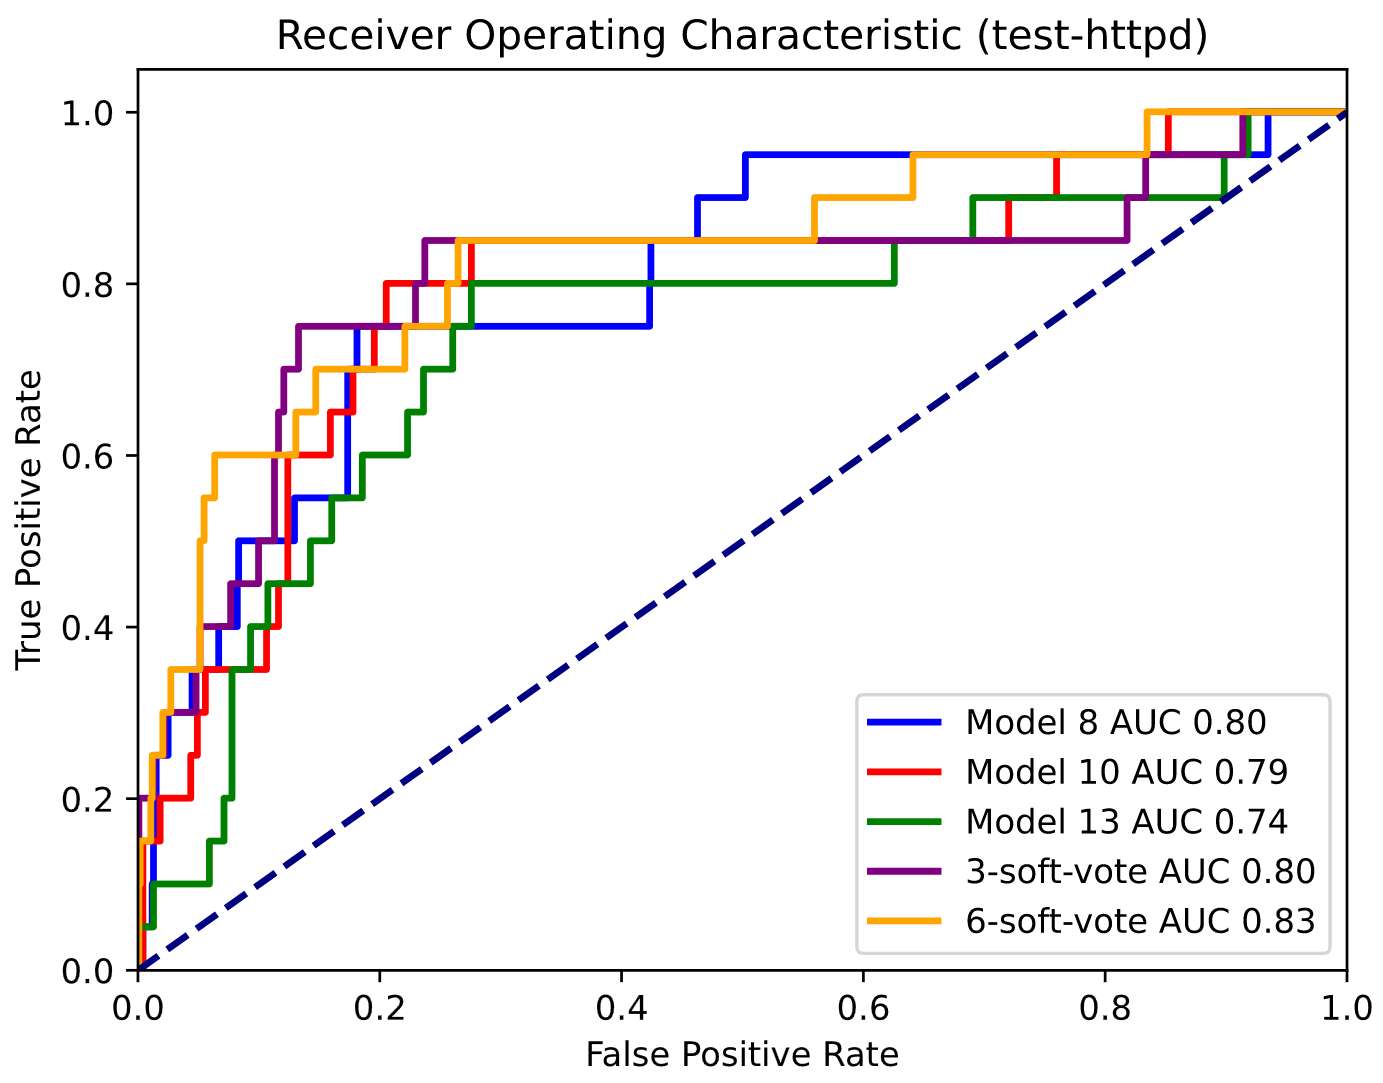
\includegraphics[width=0.75\textwidth]{figures/auc-httpd.png}
	\caption{The figure shows ROC curves for the top-performing models developed in this thesis. The models were evaluated on test data from the httpd project.}
	\label{figure:auc-httpd}
\end{figure}

\begin{figure}[ht]
	\centering
	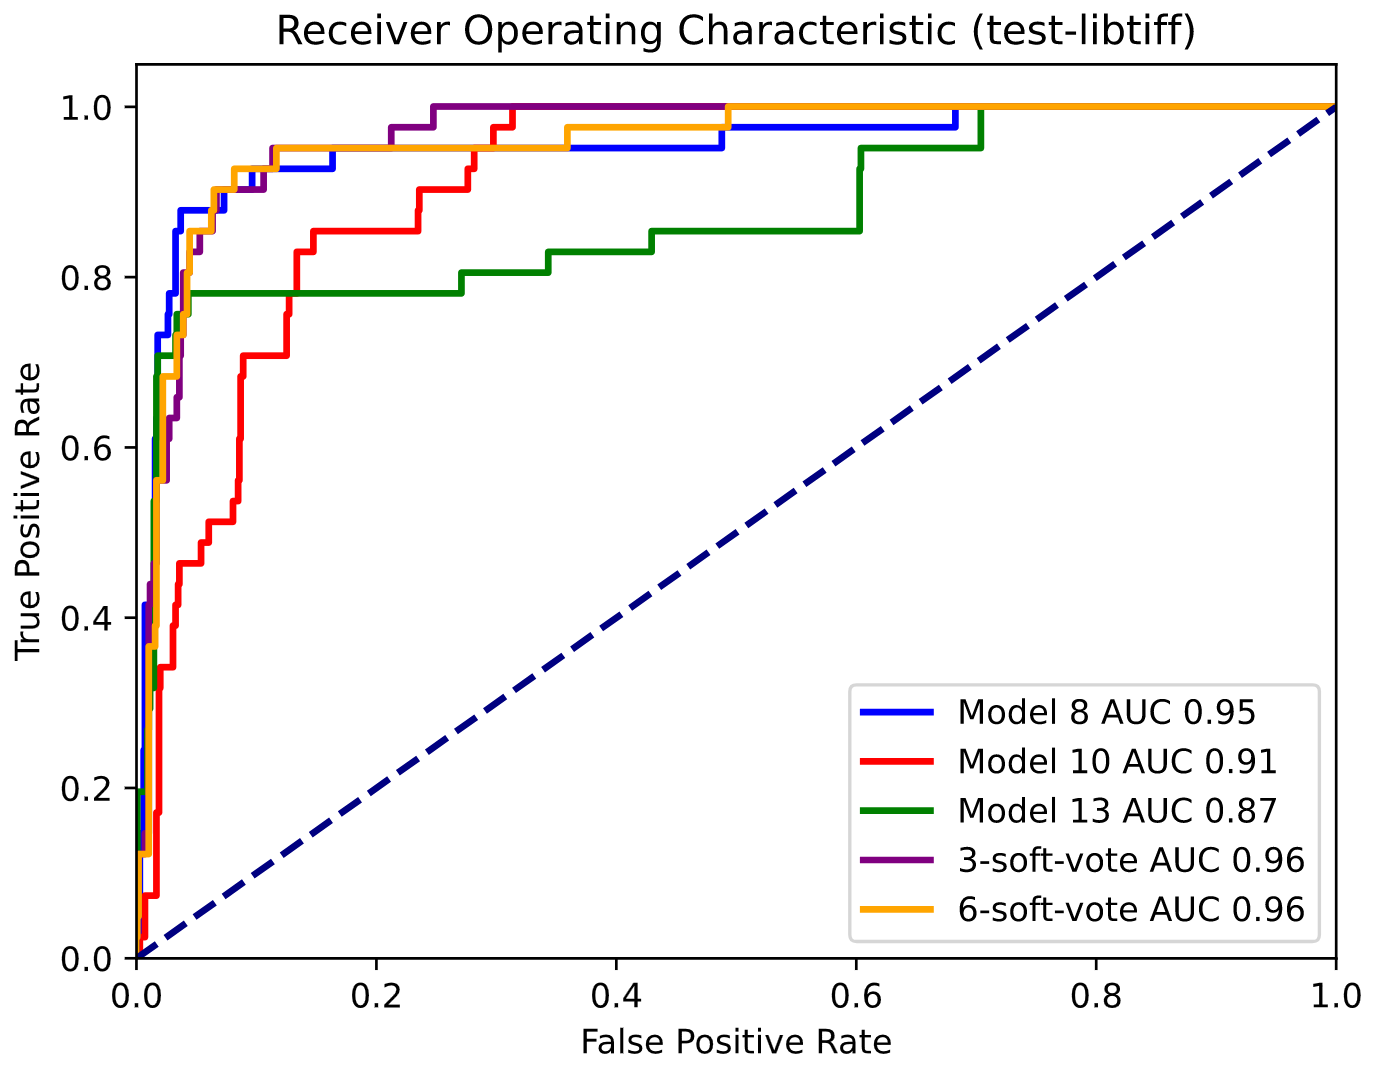
\includegraphics[width=0.75\textwidth]{figures/auc-libtiff.png}
	\caption{The figure shows ROC curves for the top-performing models developed in this thesis. The models were evaluated on test data from the libtiff project.}
	\label{figure:auc-libtiff}
\end{figure}

\begin{figure}[ht]
	\centering
	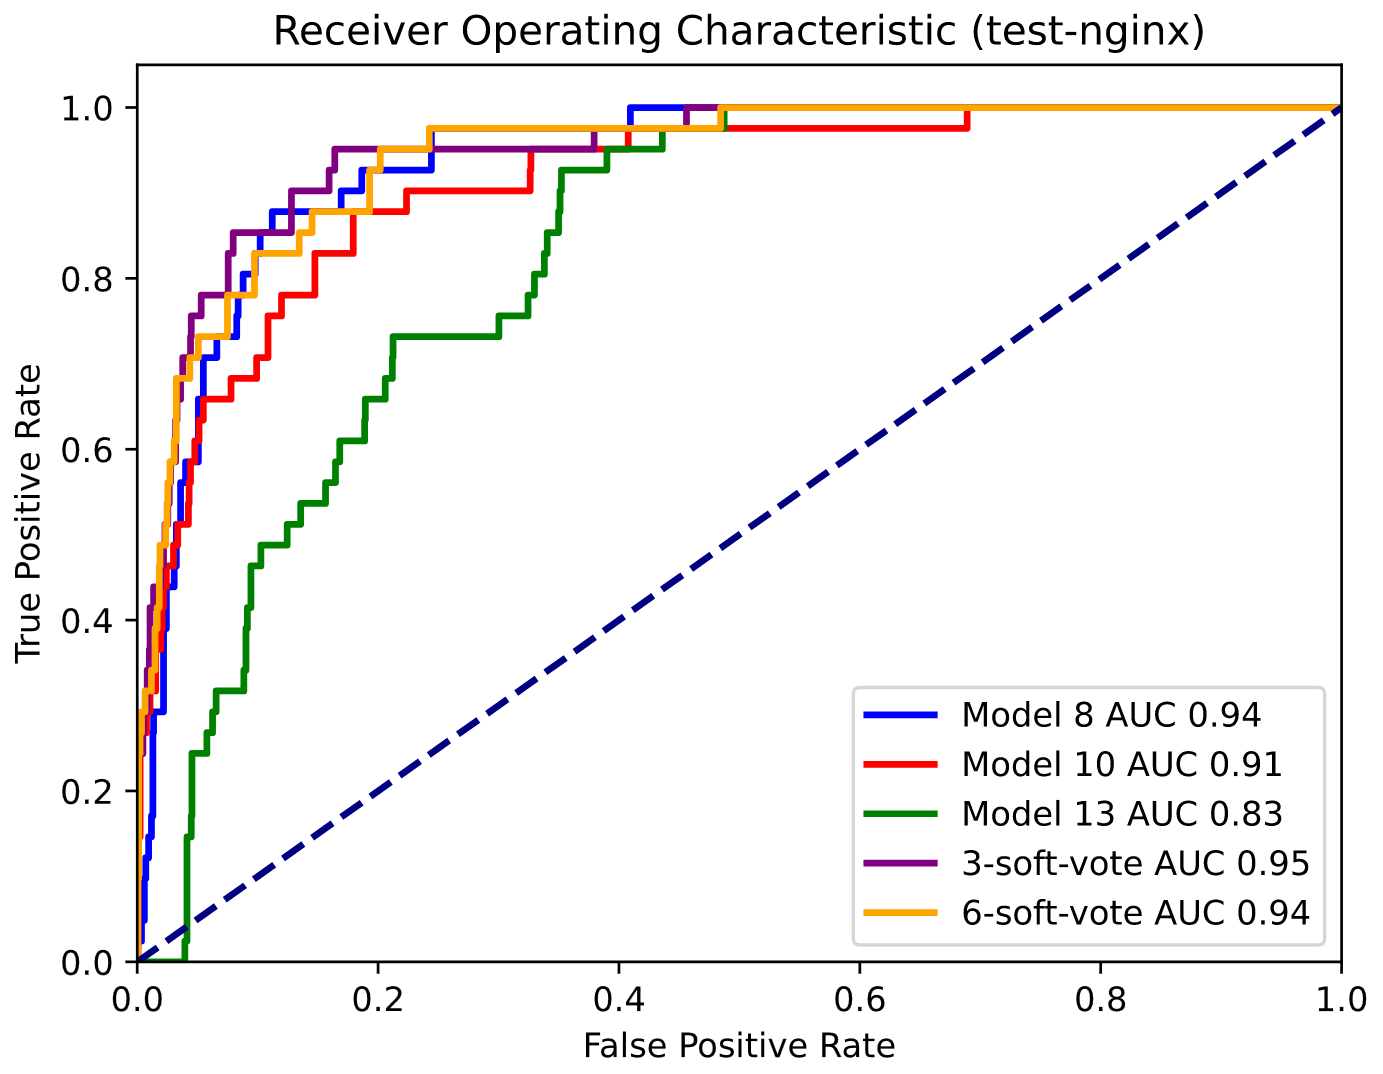
\includegraphics[width=0.75\textwidth]{figures/auc-nginx.png}
	\caption{The figure shows ROC curves for the top-performing models developed in this thesis. The models were evaluated on test data from the nginx project.}
	\label{figure:auc-nginx}
\end{figure}

\begin{figure}[ht]
	\centering
	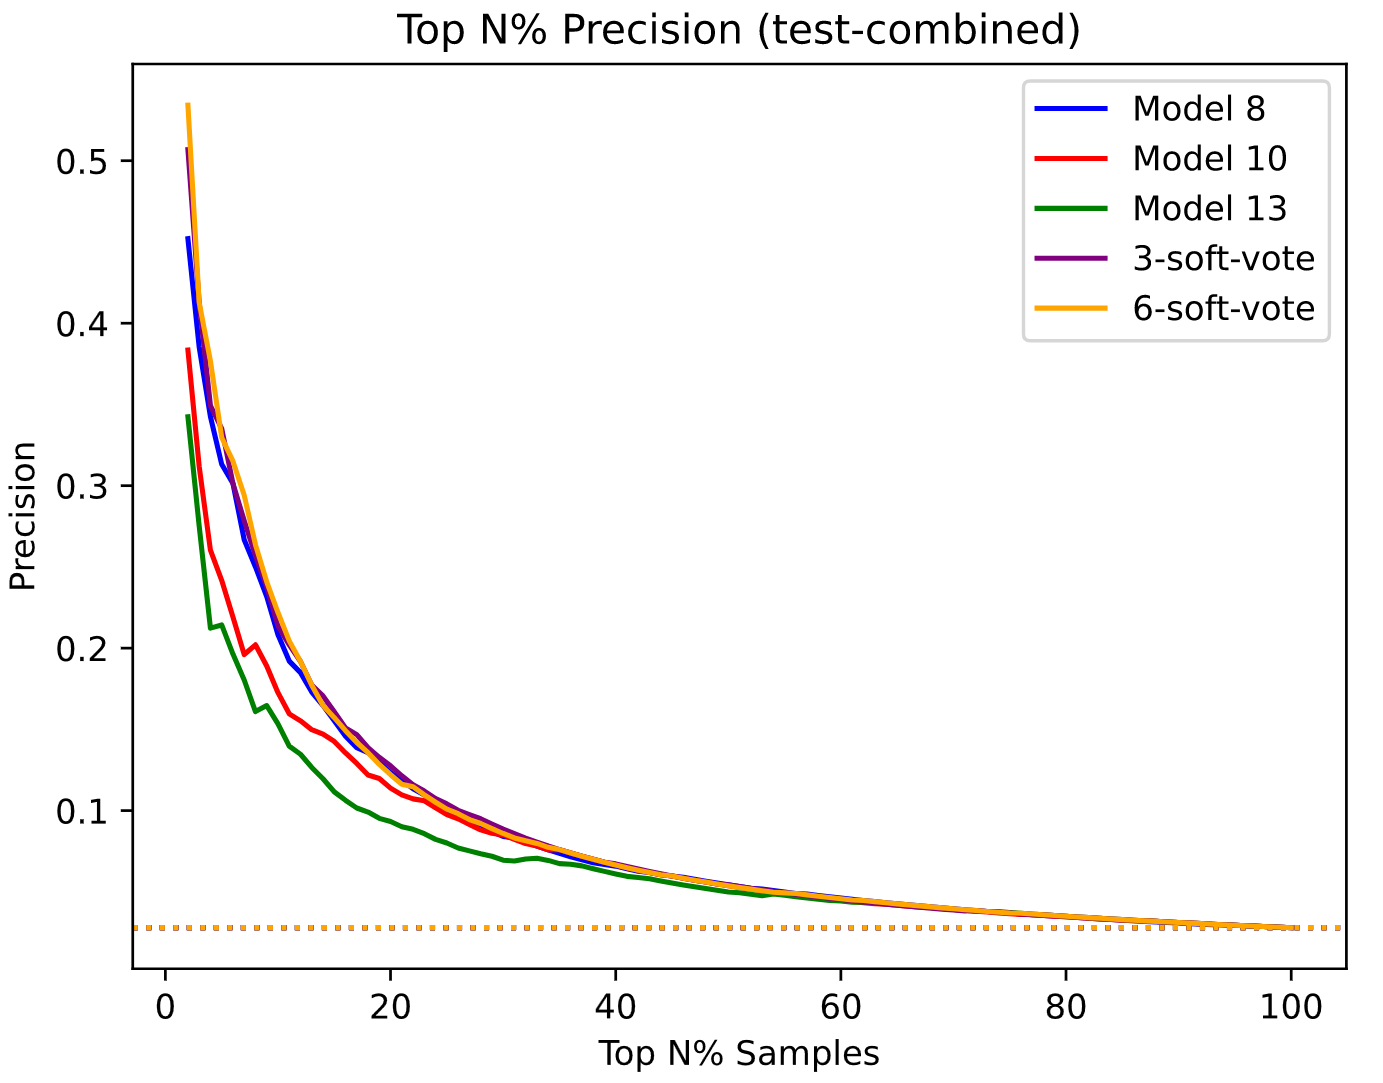
\includegraphics[width=0.75\textwidth]{figures/topn-combined.png}
	\caption{The figure shows the precision of top-performing models for various percentages of top-ranked samples. The models were evaluated on combined test data from the httpd, libtiff, and nginx projects. The dashed horizontal line indicates the precision of a random model.}
	\label{figure:topn-combined}
\end{figure}

\begin{figure}[ht]
	\centering
	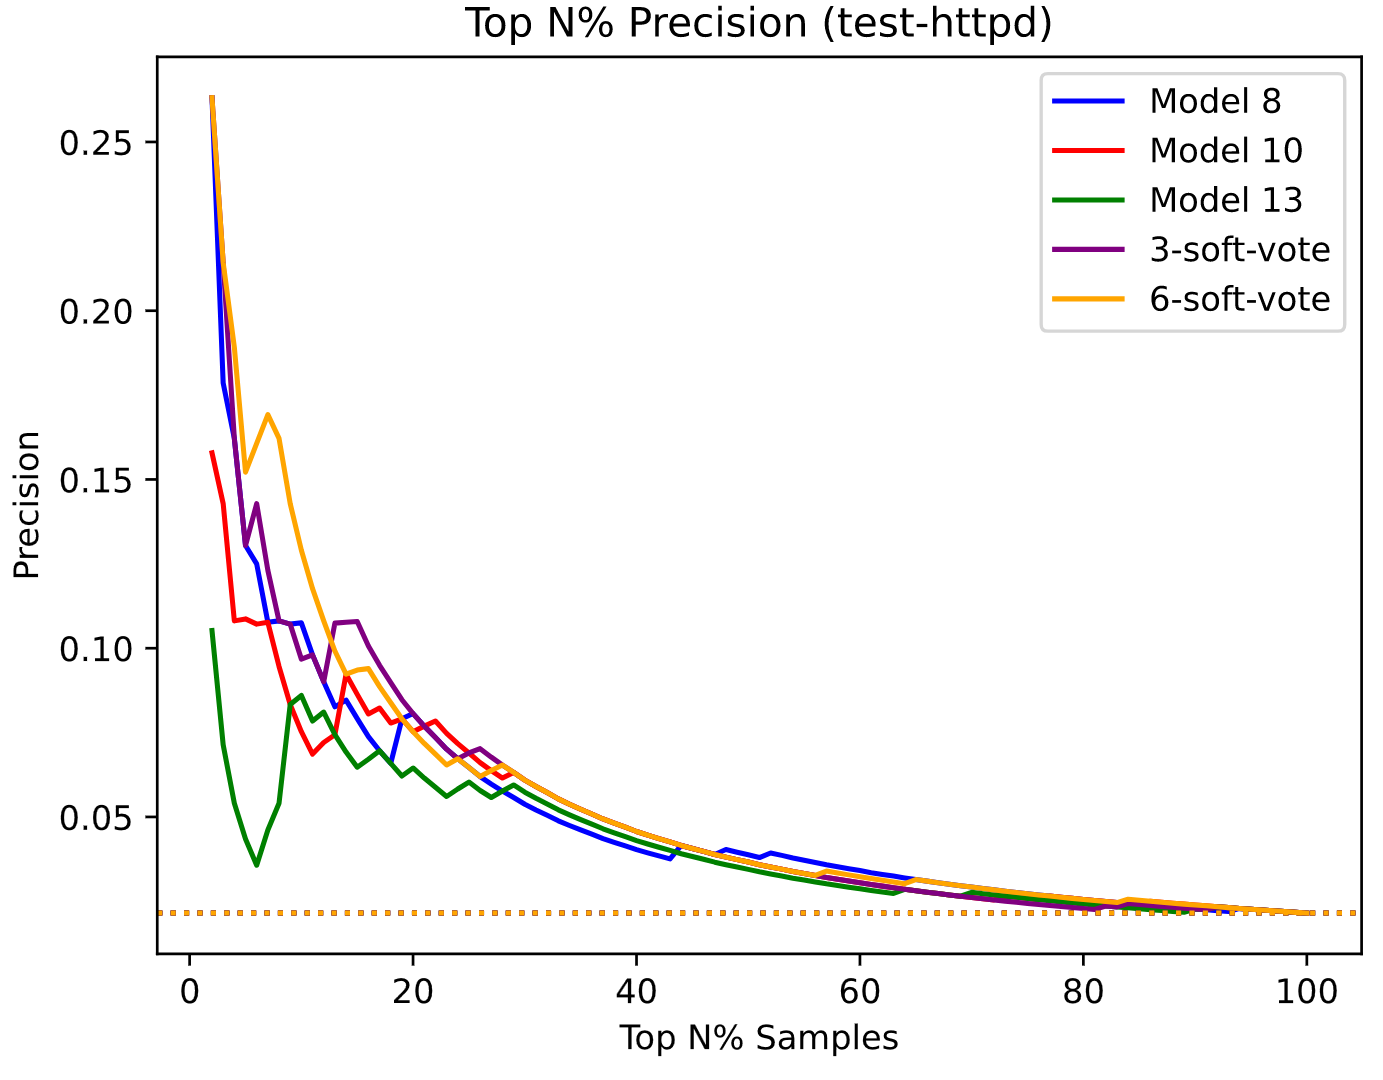
\includegraphics[width=0.75\textwidth]{figures/topn-httpd.png}
	\caption{The figure shows the precision of top-performing models for various percentages of top-ranked samples. The models were evaluated on test data from the httpd project. The dashed horizontal line indicates the precision of a random model.}
	\label{figure:topn-httpd}
\end{figure}

\begin{figure}[ht]
	\centering
	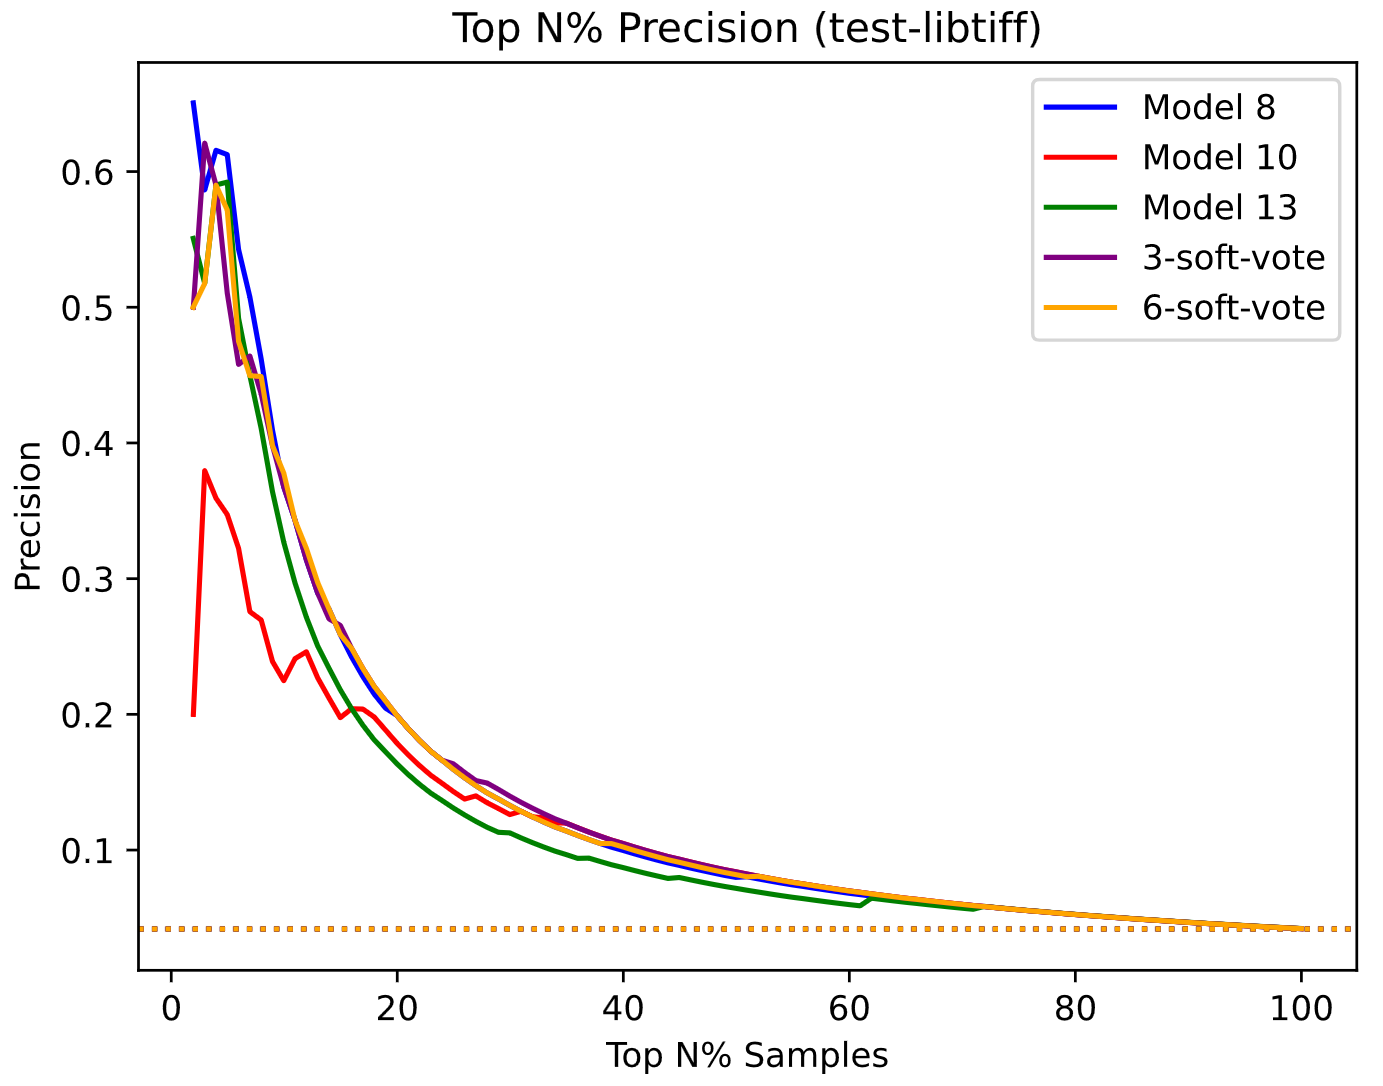
\includegraphics[width=0.75\textwidth]{figures/topn-libtiff.png}
	\caption{The figure shows the precision of top-performing models for various percentages of top-ranked samples. The models were evaluated on test data from the libtiff project. The dashed horizontal line indicates the precision of a random model.}
	\label{figure:topn-libtiff}
\end{figure}

\begin{figure}[ht]
	\centering
	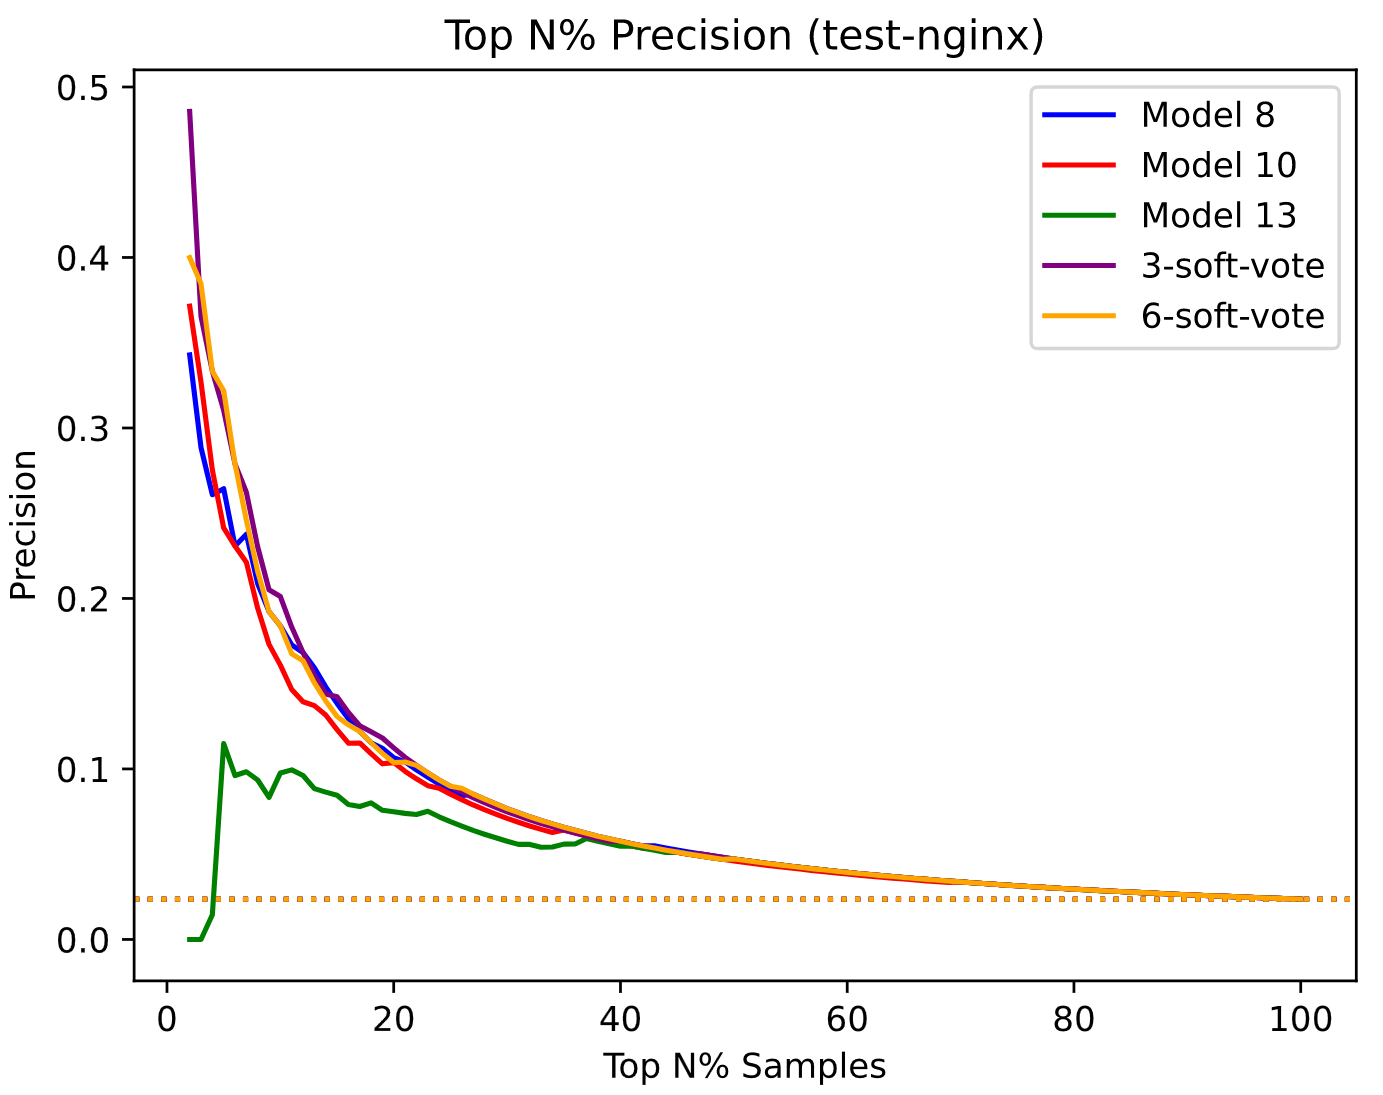
\includegraphics[width=0.75\textwidth]{figures/topn-nginx.png}
	\caption{The figure shows the precision of top-performing models for various percentages of top-ranked samples. The models were evaluated on test data from the nginx project. The dashed horizontal line indicates the precision of a random model.}
	\label{figure:topn-nginx}
\end{figure}


\begin{table}
    \centering
    \caption{The table shows all attributes for every node set present in Graph D2A. This table is divided into multiple parts by columns; this is Part 1. The remaining parts are in Tables~\ref{tab:attributes2},~\ref{tab:attributes3},~\ref{tab:attributes4},~\ref{tab:attributes5}, and~\ref{tab:attributes6}.}
    \vskip6pt
    \begin{tabular}{
        !{\vrule width 1pt}>{\centering\arraybackslash}m{1.95cm}!{\vrule width 1pt}
        >{\centering\arraybackslash}m{0.5cm}|
        >{\centering\arraybackslash}m{1cm}|
        >{\centering\arraybackslash}m{1.6cm}|
        >{\centering\arraybackslash}m{1cm}|
        >{\centering\arraybackslash}m{1.8cm}|
        >{\centering\arraybackslash}m{1.2cm}|
        >{\centering\arraybackslash}m{1cm}!{\vrule width 1pt}}
        
        \noalign{\hrule height 1pt}
        {\small Node Set} & {\scriptsize ID} & {\scriptsize LABEL} & {\scriptsize \hspace{0.2cm}LINE\newline NUMBER} & {\scriptsize CODE} & {\scriptsize \hspace{0.1cm}COLUMN\newline NUMBER} & {\scriptsize ORDER} & {\scriptsize NAME} \\
        \noalign{\hrule height 1pt}
        {\scriptsize META DATA}                                             & {\scriptsize \xmark} & {\scriptsize \xmark} & {\scriptsize -}         & {\scriptsize -} & {\scriptsize -} & {\scriptsize -} & {\scriptsize -}\\ \hline 
        {\scriptsize FILE}                                                  & {\scriptsize \xmark} & {\scriptsize \xmark} & {\scriptsize \xmark}    & {\scriptsize \xmark} & {\scriptsize \xmark} & {\scriptsize \xmark} & {\scriptsize \xmark}\\ \hline 
        {\scriptsize NAMESPACE}                                             & {\scriptsize \xmark} & {\scriptsize \xmark} & {\scriptsize \xmark}    & {\scriptsize \xmark} & {\scriptsize \xmark} & {\scriptsize \xmark} & {\scriptsize \xmark}\\ \hline 
        {\scriptsize NAMESPACE\newline BLOCK}                               & {\scriptsize \xmark} & {\scriptsize \xmark} & {\scriptsize \xmark}    & {\scriptsize \xmark} & {\scriptsize \xmark} & {\scriptsize \xmark} & {\scriptsize \xmark}\\ \hline 
        {\scriptsize METHOD}                                                & {\scriptsize \xmark} & {\scriptsize \checkmark} & {\scriptsize \xmark} & {\scriptsize \xmark} & {\scriptsize \xmark} & {\scriptsize \checkmark} & {\scriptsize \xmark}\\ \hline 
        {\scriptsize \hspace{0.02cm} METHOD\newline PARAMETER\newline IN}  & {\scriptsize \xmark} & {\scriptsize \checkmark} & {\scriptsize \xmark} & {\scriptsize \xmark} & {\scriptsize \xmark} & {\scriptsize \checkmark} & {\scriptsize \xmark}\\ \hline 
        {\scriptsize \hspace{0.02cm} METHOD\newline PARAMETER\newline OUT}   & {\scriptsize \xmark} & {\scriptsize \xmark} & {\scriptsize \xmark}    & {\scriptsize \xmark} & {\scriptsize \xmark} & {\scriptsize \xmark} & {\scriptsize \xmark}\\ \hline 
        {\scriptsize \hspace{0.02cm} METHOD\newline RETURN}                 & {\scriptsize \xmark} & {\scriptsize \checkmark} & {\scriptsize \xmark} & {\scriptsize \xmark} & {\scriptsize \xmark} & {\scriptsize \checkmark} & {\scriptsize -}\\ \hline 
        {\scriptsize MEMBER}                                                & {\scriptsize \xmark} & {\scriptsize \checkmark} & {\scriptsize \xmark} & {\scriptsize \xmark} & {\scriptsize \xmark} & {\scriptsize \checkmark} & {\scriptsize \xmark}\\ \hline 
        {\scriptsize TYPE}                                                  & {\scriptsize \xmark} & {\scriptsize \checkmark} & {\scriptsize -}     & {\scriptsize -} & {\scriptsize -} & {\scriptsize -} & {\scriptsize \xmark}\\ \hline 
        {\scriptsize TYPE DECL}                                             & {\scriptsize \xmark} & {\scriptsize \xmark} & {\scriptsize \xmark}    & {\scriptsize \xmark} & {\scriptsize \xmark} & {\scriptsize \xmark} & {\scriptsize \xmark}\\ \hline 
        {\scriptsize BLOCK}                                                 & {\scriptsize \xmark} & {\scriptsize \checkmark} & {\scriptsize \xmark} & {\scriptsize \xmark} & {\scriptsize \xmark} & {\scriptsize \checkmark} & {\scriptsize -}\\ \hline 
        {\scriptsize CALL}                                                  & {\scriptsize \xmark} & {\scriptsize \checkmark} & {\scriptsize \xmark} & {\scriptsize \xmark} & {\scriptsize \xmark} & {\scriptsize \checkmark} & {\scriptsize \xmark}\\ \hline 
        {\scriptsize \hspace{0.02cm} FIELD\newline IDENTIFIER}              & {\scriptsize \xmark} & {\scriptsize \checkmark} & {\scriptsize \xmark} & {\scriptsize \xmark} & {\scriptsize \xmark} & {\scriptsize \checkmark} & {\scriptsize -}\\ \hline 
        {\scriptsize IDENTIFIER}                                            & {\scriptsize \xmark} & {\scriptsize \checkmark} & {\scriptsize \xmark} & {\scriptsize \xmark} & {\scriptsize \xmark} & {\scriptsize \checkmark} & {\scriptsize \xmark}\\ \hline 
        {\scriptsize LITERAL}                                               & {\scriptsize \xmark} & {\scriptsize \checkmark} & {\scriptsize \xmark} & {\scriptsize \checkmark} & {\scriptsize \xmark} & {\scriptsize \checkmark} & {\scriptsize -}\\ \hline 
        {\scriptsize LOCAL}                                                 & {\scriptsize \xmark} & {\scriptsize \checkmark} & {\scriptsize \xmark} & {\scriptsize \xmark} & {\scriptsize \xmark} & {\scriptsize \checkmark} & {\scriptsize \xmark}\\ \hline 
        {\scriptsize \hspace{0.02cm} METHOD\newline REF}                    & {\scriptsize \xmark} & {\scriptsize \checkmark} & {\scriptsize \xmark} & {\scriptsize \xmark} & {\scriptsize \xmark} & {\scriptsize \checkmark} & {\scriptsize -}\\ \hline 
        {\scriptsize RETURN}                                                & {\scriptsize \xmark} & {\scriptsize \checkmark} & {\scriptsize \xmark} & {\scriptsize \xmark} & {\scriptsize \xmark} & {\scriptsize \checkmark} & {\scriptsize -}\\ \hline 
        {\scriptsize UNKNOWN}                                               & {\scriptsize \xmark} & {\scriptsize \checkmark} & {\scriptsize \xmark} & {\scriptsize \xmark} & {\scriptsize \xmark} & {\scriptsize \checkmark} & {\scriptsize -}\\ \hline 
        \noalign{\hrule height 1pt}
    \end{tabular}
    \label{tab:attributes1}
\end{table}










\begin{table}
    \centering
    \caption{The table shows all attributes for every node set present in Graph D2A. This table is divided into multiple parts by columns; this is Part 2. The remaining parts are in Tables~\ref{tab:attributes1},~\ref{tab:attributes3},~\ref{tab:attributes4},~\ref{tab:attributes5}, and~\ref{tab:attributes6}.}
    \vskip6pt
    \begin{tabular}{
        !{\vrule width 1pt}>{\centering\arraybackslash}m{1.95cm}!{\vrule width 1pt}
        >{\centering\arraybackslash}m{1.8cm}|
        >{\centering\arraybackslash}m{1.8cm}|
        >{\centering\arraybackslash}m{0.9cm}|
        >{\centering\arraybackslash}m{2.8cm}|
        >{\centering\arraybackslash}m{1.7cm}|
        >{\centering\arraybackslash}m{0.9cm}!{\vrule width 1pt}}
        
        \noalign{\hrule height 1pt}
        {\small Node Set} & {\scriptsize ARGUMENT \newline INDEX} & {\scriptsize ARGUMENT\newline NAME} & {\scriptsize TYPE\newline FULL\newline NAME} & {\scriptsize \hspace{0.1cm}DYNAMIC TYPE\newline HINT FULL NAME} & {\scriptsize FILENAME} & {\scriptsize \hspace{0.05cm}FULL\newline NAME} \\
        \noalign{\hrule height 1pt}
        {\scriptsize META DATA}                                             & {\scriptsize -} & {\scriptsize -} & {\scriptsize -} & {\scriptsize -} & {\scriptsize -} & {\scriptsize -} \\ \hline 
        {\scriptsize FILE}                                                  & {\scriptsize -} & {\scriptsize -} & {\scriptsize -} & {\scriptsize -} & {\scriptsize -} & {\scriptsize -} \\ \hline 
        {\scriptsize NAMESPACE}                                             & {\scriptsize -} & {\scriptsize -} & {\scriptsize -} & {\scriptsize -} & {\scriptsize -} & {\scriptsize -} \\ \hline 
        {\scriptsize NAMESPACE\newline BLOCK}                               & {\scriptsize -} & {\scriptsize -} & {\scriptsize -} & {\scriptsize -} & {\scriptsize \xmark} & {\scriptsize \xmark} \\ \hline 
        {\scriptsize METHOD}                                                & {\scriptsize -} & {\scriptsize -} & {\scriptsize -} & {\scriptsize -} & {\scriptsize \xmark} & {\scriptsize \checkmark} \\ \hline 
        {\scriptsize \hspace{0.02cm} METHOD\newline PARAMETER\newline IN}  & {\scriptsize -} & {\scriptsize -} & {\scriptsize \xmark} & {\scriptsize \xmark} & {\scriptsize -} & {\scriptsize -} \\ \hline 
        {\scriptsize \hspace{0.02cm} METHOD\newline PARAMETER\newline OUT}   & {\scriptsize -} & {\scriptsize -} & {\scriptsize \xmark} & {\scriptsize -} & {\scriptsize -} & {\scriptsize -} \\ \hline 
        {\scriptsize \hspace{0.02cm} METHOD\newline RETURN}                 & {\scriptsize -} & {\scriptsize -} & {\scriptsize \xmark} & {\scriptsize \xmark} & {\scriptsize -} & {\scriptsize -} \\ \hline 
        {\scriptsize MEMBER}                                                & {\scriptsize -} & {\scriptsize -} & {\scriptsize \xmark} & {\scriptsize \xmark} & {\scriptsize -} & {\scriptsize -} \\ \hline 
        {\scriptsize TYPE}                                                  & {\scriptsize -} & {\scriptsize -} & {\scriptsize -} & {\scriptsize -} & {\scriptsize -} & {\scriptsize \checkmark} \\ \hline 
        {\scriptsize TYPE DECL}                                             & {\scriptsize -} & {\scriptsize -} & {\scriptsize -} & {\scriptsize -} & {\scriptsize \xmark} & {\scriptsize \xmark} \\ \hline 
        {\scriptsize BLOCK}                                                 & {\scriptsize \checkmark} & {\scriptsize \xmark} & {\scriptsize \xmark} & {\scriptsize \xmark} & {\scriptsize -} & {\scriptsize -} \\ \hline 
        {\scriptsize CALL}                                                  & {\scriptsize \checkmark} & {\scriptsize \xmark} & {\scriptsize \xmark} & {\scriptsize \xmark} & {\scriptsize -} & {\scriptsize -} \\ \hline 
        {\scriptsize \hspace{0.02cm} FIELD\newline IDENTIFIER}              & {\scriptsize \checkmark} & {\scriptsize \xmark} & {\scriptsize -} & {\scriptsize -} & {\scriptsize -} & {\scriptsize -} \\ \hline 
        {\scriptsize IDENTIFIER}                                            & {\scriptsize \checkmark} & {\scriptsize \xmark} & {\scriptsize \xmark} & {\scriptsize \xmark} & {\scriptsize -} & {\scriptsize -} \\ \hline 
        {\scriptsize LITERAL}                                               & {\scriptsize \checkmark} & {\scriptsize \xmark} & {\scriptsize \xmark} & {\scriptsize \xmark} & {\scriptsize -} & {\scriptsize -} \\ \hline 
        {\scriptsize LOCAL}                                                 & {\scriptsize -} & {\scriptsize -} & {\scriptsize \xmark} & {\scriptsize \xmark} & {\scriptsize -} & {\scriptsize -} \\ \hline 
        {\scriptsize \hspace{0.02cm} METHOD\newline REF}                    & {\scriptsize \checkmark} & {\scriptsize \xmark} & {\scriptsize \xmark} & {\scriptsize \xmark} & {\scriptsize -} & {\scriptsize -} \\ \hline 
        {\scriptsize RETURN}                                                & {\scriptsize \checkmark} & {\scriptsize \xmark} & {\scriptsize -} & {\scriptsize -} & {\scriptsize -} & {\scriptsize -} \\ \hline 
        {\scriptsize UNKNOWN}                                               & {\scriptsize \checkmark} & {\scriptsize \xmark} & {\scriptsize \xmark} & {\scriptsize \xmark} & {\scriptsize -} & {\scriptsize -} \\ \hline 
        \noalign{\hrule height 1pt}
    \end{tabular}
    \label{tab:attributes2}
\end{table}

\begin{table}
    \centering
    \caption{The table shows all attributes for every node set present in Graph D2A. This table is divided into multiple parts by columns; this is Part 3. The remaining parts are in Tables~\ref{tab:attributes1},~\ref{tab:attributes2},~\ref{tab:attributes4},~\ref{tab:attributes5}, and~\ref{tab:attributes6}.}
    \vskip6pt
    \begin{tabular}{
        !{\vrule width 1pt}>{\centering\arraybackslash}m{1.95cm}!{\vrule width 1pt}
        >{\centering\arraybackslash}m{1.8cm}|
        >{\centering\arraybackslash}m{1.5cm}|
        >{\centering\arraybackslash}m{1.5cm}|
        >{\centering\arraybackslash}m{2cm}|
        >{\centering\arraybackslash}m{1cm}|
        >{\centering\arraybackslash}m{2.5cm}!{\vrule width 1pt}}
        
        \noalign{\hrule height 1pt}
        {\small Node Set} & {\scriptsize SIGNATURE} & {\scriptsize \hspace{0.05cm}METHOD\newline \hspace{0.1cm}FULL\newline NAME} & {\scriptsize \hspace{0.1cm}PARSER\newline TYPE\newline NAME} & {\scriptsize EVALUATION\newline STRATEGY} & {\scriptsize HASH} & {\scriptsize \hspace{0.15cm}AST PARENT \newline FULL NAME}\\
        \noalign{\hrule height 1pt}
        {\scriptsize META DATA}                                             & {\scriptsize -} & {\scriptsize -} & {\scriptsize -} & {\scriptsize -} & {\scriptsize \xmark} & {\scriptsize -} \\ \hline 
        {\scriptsize FILE}                                                  & {\scriptsize -} & {\scriptsize -} & {\scriptsize -} & {\scriptsize -} & {\scriptsize \xmark} & {\scriptsize -} \\ \hline 
        {\scriptsize NAMESPACE}                                             & {\scriptsize -} & {\scriptsize -} & {\scriptsize -} & {\scriptsize -} & {\scriptsize -} & {\scriptsize -} \\ \hline 
        {\scriptsize NAMESPACE\newline BLOCK}                               & {\scriptsize -} & {\scriptsize -} & {\scriptsize -} & {\scriptsize -} & {\scriptsize -} & {\scriptsize -} \\ \hline 
        {\scriptsize METHOD}                                                & {\scriptsize \xmark} & {\scriptsize -} & {\scriptsize -} & {\scriptsize -} & {\scriptsize \xmark} & {\scriptsize \xmark} \\ \hline 
        {\scriptsize \hspace{0.02cm} METHOD\newline PARAMETER\newline IN}  & {\scriptsize -} & {\scriptsize -} & {\scriptsize -} & {\scriptsize \xmark} & {\scriptsize -} & {\scriptsize -} \\ \hline 
        {\scriptsize \hspace{0.02cm} METHOD\newline PARAMETER\newline OUT}   & {\scriptsize -} & {\scriptsize -} & {\scriptsize -} & {\scriptsize \xmark} & {\scriptsize -} & {\scriptsize -} \\ \hline 
        {\scriptsize \hspace{0.02cm} METHOD\newline RETURN}                 & {\scriptsize -} & {\scriptsize -} & {\scriptsize -} & {\scriptsize \xmark} & {\scriptsize -} & {\scriptsize -} \\ \hline 
        {\scriptsize MEMBER}                                                & {\scriptsize -} & {\scriptsize -} & {\scriptsize -} & {\scriptsize -} & {\scriptsize -} & {\scriptsize -} \\ \hline 
        {\scriptsize TYPE}                                                  & {\scriptsize -} & {\scriptsize -} & {\scriptsize -} & {\scriptsize -} & {\scriptsize -} & {\scriptsize -} \\ \hline 
        {\scriptsize TYPE DECL}                                             & {\scriptsize -} & {\scriptsize -} & {\scriptsize -} & {\scriptsize -} & {\scriptsize -} & {\scriptsize \xmark} \\ \hline 
        {\scriptsize BLOCK}                                                 & {\scriptsize -} & {\scriptsize -} & {\scriptsize -} & {\scriptsize -} & {\scriptsize -} & {\scriptsize -} \\ \hline 
        {\scriptsize CALL}                                                  & {\scriptsize \xmark} & {\scriptsize \xmark} & {\scriptsize -} & {\scriptsize -} & {\scriptsize -} & {\scriptsize -} \\ \hline 
        {\scriptsize \hspace{0.02cm} FIELD\newline IDENTIFIER}              & {\scriptsize -} & {\scriptsize -} & {\scriptsize -} & {\scriptsize -} & {\scriptsize -} & {\scriptsize -} \\ \hline 
        {\scriptsize IDENTIFIER}                                            & {\scriptsize -} & {\scriptsize -} & {\scriptsize -} & {\scriptsize -} & {\scriptsize -} & {\scriptsize -} \\ \hline 
        {\scriptsize LITERAL}                                               & {\scriptsize -} & {\scriptsize -} & {\scriptsize -} & {\scriptsize -} & {\scriptsize -} & {\scriptsize -} \\ \hline 
        {\scriptsize LOCAL}                                                 & {\scriptsize -} & {\scriptsize -} & {\scriptsize -} & {\scriptsize -} & {\scriptsize -} & {\scriptsize -} \\ \hline 
        {\scriptsize \hspace{0.02cm} METHOD\newline REF}                    & {\scriptsize -} & {\scriptsize \xmark} & {\scriptsize -} & {\scriptsize -} & {\scriptsize -} & {\scriptsize -} \\ \hline 
        {\scriptsize RETURN}                                                & {\scriptsize -} & {\scriptsize -} & {\scriptsize -} & {\scriptsize -} & {\scriptsize -} & {\scriptsize -} \\ \hline 
        {\scriptsize UNKNOWN}                                               & {\scriptsize -} & {\scriptsize -} & {\scriptsize \xmark} & {\scriptsize -} & {\scriptsize -} & {\scriptsize -} \\ \hline 
        \noalign{\hrule height 1pt}
    \end{tabular}
    \label{tab:attributes3}
\end{table}


\begin{table}
    \centering
    \caption{The table shows all attributes for every node set present in Graph D2A. This table is divided into multiple parts by columns; this is Part 4. The remaining parts are in Tables~\ref{tab:attributes1},~\ref{tab:attributes2},~\ref{tab:attributes3},~\ref{tab:attributes5}, and~\ref{tab:attributes6}.}
    \vskip6pt
    \begin{tabular}{
        !{\vrule width 1pt}>{\centering\arraybackslash}m{1.95cm}!{\vrule width 1pt}
        >{\centering\arraybackslash}m{1.2cm}|
        >{\centering\arraybackslash}m{1.8cm}|
        >{\centering\arraybackslash}m{1.1cm}|
        >{\centering\arraybackslash}m{1.6cm}|
        >{\centering\arraybackslash}m{1.4cm}|
        >{\centering\arraybackslash}m{1.6cm}!{\vrule width 1pt}}
        
        \noalign{\hrule height 1pt}
        {\small Node Set} & {\scriptsize \hspace{0.1cm}AST\newline PARENT\newline TYPE} & {\scriptsize \hspace{0.3cm}IS\newline EXTERNAL} & {\scriptsize INDEX} & {\scriptsize \hspace{0.3cm}IS\newline VARIADIC} & {\scriptsize COLUMN\newline NUMBER\newline END} & {\scriptsize \hspace{0.2cm}LINE\newline NUMBER\newline END}\\
        \noalign{\hrule height 1pt}
        {\scriptsize META DATA}                                             & {\scriptsize -} & {\scriptsize -} & {\scriptsize -} & {\scriptsize -} & {\scriptsize -} & {\scriptsize -} \\ \hline 
        {\scriptsize FILE}                                                  & {\scriptsize -} & {\scriptsize -} & {\scriptsize -} & {\scriptsize -} & {\scriptsize -} & {\scriptsize -} \\ \hline 
        {\scriptsize NAMESPACE}                                             & {\scriptsize -} & {\scriptsize -} & {\scriptsize -} & {\scriptsize -} & {\scriptsize -} & {\scriptsize -} \\ \hline 
        {\scriptsize NAMESPACE\newline BLOCK}                               & {\scriptsize -} & {\scriptsize -} & {\scriptsize -} & {\scriptsize -} & {\scriptsize -} & {\scriptsize -} \\ \hline 
        {\scriptsize METHOD}                                                & {\scriptsize \xmark} & {\scriptsize \checkmark} & {\scriptsize -} & {\scriptsize -} & {\scriptsize \xmark} & {\scriptsize \xmark} \\ \hline 
        {\scriptsize \hspace{0.02cm} METHOD\newline PARAMETER\newline IN}  & {\scriptsize -} & {\scriptsize -} & {\scriptsize \xmark} & {\scriptsize \xmark} & {\scriptsize -} & {\scriptsize -} \\ \hline 
        {\scriptsize \hspace{0.02cm} METHOD\newline PARAMETER\newline OUT}   & {\scriptsize -} & {\scriptsize -} & {\scriptsize \xmark} & {\scriptsize \xmark} & {\scriptsize -} & {\scriptsize -} \\ \hline 
        {\scriptsize \hspace{0.02cm} METHOD\newline RETURN}                 & {\scriptsize -} & {\scriptsize -} & {\scriptsize -} & {\scriptsize -} & {\scriptsize -} & {\scriptsize -} \\ \hline 
        {\scriptsize MEMBER}                                                & {\scriptsize -} & {\scriptsize -} & {\scriptsize -} & {\scriptsize -} & {\scriptsize -} & {\scriptsize -} \\ \hline 
        {\scriptsize TYPE}                                                  & {\scriptsize -} & {\scriptsize -} & {\scriptsize -} & {\scriptsize -} & {\scriptsize -} & {\scriptsize -} \\ \hline 
        {\scriptsize TYPE DECL}                                             & {\scriptsize \xmark} & {\scriptsize \xmark} & {\scriptsize -} & {\scriptsize -} & {\scriptsize -} & {\scriptsize -} \\ \hline 
        {\scriptsize BLOCK}                                                 & {\scriptsize -} & {\scriptsize -} & {\scriptsize -} & {\scriptsize -} & {\scriptsize -} & {\scriptsize -} \\ \hline 
        {\scriptsize CALL}                                                  & {\scriptsize -} & {\scriptsize -} & {\scriptsize -} & {\scriptsize -} & {\scriptsize -} & {\scriptsize -} \\ \hline 
        {\scriptsize \hspace{0.02cm} FIELD\newline IDENTIFIER}              & {\scriptsize -} & {\scriptsize -} & {\scriptsize -} & {\scriptsize -} & {\scriptsize -} & {\scriptsize -} \\ \hline 
        {\scriptsize IDENTIFIER}                                            & {\scriptsize -} & {\scriptsize -} & {\scriptsize -} & {\scriptsize -} & {\scriptsize -} & {\scriptsize -} \\ \hline 
        {\scriptsize LITERAL}                                               & {\scriptsize -} & {\scriptsize -} & {\scriptsize -} & {\scriptsize -} & {\scriptsize -} & {\scriptsize -} \\ \hline 
        {\scriptsize LOCAL}                                                 & {\scriptsize -} & {\scriptsize -} & {\scriptsize -} & {\scriptsize -} & {\scriptsize -} & {\scriptsize -} \\ \hline 
        {\scriptsize \hspace{0.02cm} METHOD\newline REF}                    & {\scriptsize -} & {\scriptsize -} & {\scriptsize -} & {\scriptsize -} & {\scriptsize -} & {\scriptsize -} \\ \hline 
        {\scriptsize RETURN}                                                & {\scriptsize -} & {\scriptsize -} & {\scriptsize -} & {\scriptsize -} & {\scriptsize -} & {\scriptsize -} \\ \hline 
        {\scriptsize UNKNOWN}                                               & {\scriptsize -} & {\scriptsize -} & {\scriptsize -} & {\scriptsize -} & {\scriptsize -} & {\scriptsize -} \\ \hline 
        \noalign{\hrule height 1pt}
    \end{tabular}
    \label{tab:attributes4}
\end{table}


\begin{table}
    \centering
    \caption{The table shows all attributes for every node set present in Graph D2A. This table is divided into multiple parts by columns; this is Part 5. The remaining parts are in Tables~\ref{tab:attributes1},~\ref{tab:attributes2},~\ref{tab:attributes3},~\ref{tab:attributes4}, and~\ref{tab:attributes6}.}
    \vskip6pt
    \begin{tabular}{
        !{\vrule width 1pt}>{\centering\arraybackslash}m{1.95cm}!{\vrule width 1pt}
        >{\centering\arraybackslash}m{1cm}|
        >{\centering\arraybackslash}m{1cm}|
        >{\centering\arraybackslash}m{1.8cm}|
        >{\centering\arraybackslash}m{1.5cm}|
        >{\centering\arraybackslash}m{1.9cm}|
        >{\centering\arraybackslash}m{1.5cm}!{\vrule width 1pt}}
        
        \noalign{\hrule height 1pt}
        {\small Node Set} & {\scriptsize TYPE\newline DECL\newline FULL\newline NAME} & {\scriptsize ALIAS\newline TYPE\newline FULL\newline NAME} & {\scriptsize CONTAINED\newline REF} & {\scriptsize CLOSURE\newline BINDING\newline ID} & {\scriptsize CANONICAL\newline NAME} & {\scriptsize DISPATCH\newline TYPE}\\
        \noalign{\hrule height 1pt}
        {\scriptsize META DATA}                                             & {\scriptsize -} & {\scriptsize -} & {\scriptsize -} & {\scriptsize -} & {\scriptsize -} & {\scriptsize -} \\ \hline 
        {\scriptsize FILE}                                                  & {\scriptsize -} & {\scriptsize -} & {\scriptsize -} & {\scriptsize -} & {\scriptsize -} & {\scriptsize -} \\ \hline 
        {\scriptsize NAMESPACE}                                             & {\scriptsize -} & {\scriptsize -} & {\scriptsize -} & {\scriptsize -} & {\scriptsize -} & {\scriptsize -} \\ \hline 
        {\scriptsize NAMESPACE\newline BLOCK}                               & {\scriptsize -} & {\scriptsize -} & {\scriptsize -} & {\scriptsize -} & {\scriptsize -} & {\scriptsize -} \\ \hline 
        {\scriptsize METHOD}                                                & {\scriptsize -} & {\scriptsize -} & {\scriptsize -} & {\scriptsize -} & {\scriptsize -} & {\scriptsize -} \\ \hline 
        {\scriptsize \hspace{0.02cm} METHOD\newline PARAMETER\newline IN}  & {\scriptsize -} & {\scriptsize -} & {\scriptsize -} & {\scriptsize -} & {\scriptsize -} & {\scriptsize -} \\ \hline 
        {\scriptsize \hspace{0.02cm} METHOD\newline PARAMETER\newline OUT}   & {\scriptsize -} & {\scriptsize -} & {\scriptsize -} & {\scriptsize -} & {\scriptsize -} & {\scriptsize -} \\ \hline 
        {\scriptsize \hspace{0.02cm} METHOD\newline RETURN}                 & {\scriptsize -} & {\scriptsize -} & {\scriptsize -} & {\scriptsize -} & {\scriptsize -} & {\scriptsize -} \\ \hline 
        {\scriptsize MEMBER}                                                & {\scriptsize -} & {\scriptsize -} & {\scriptsize -} & {\scriptsize -} & {\scriptsize -} & {\scriptsize -} \\ \hline 
        {\scriptsize TYPE}                                                  & {\scriptsize \xmark} & {\scriptsize -} & {\scriptsize -} & {\scriptsize -} & {\scriptsize -} & {\scriptsize -} \\ \hline 
        {\scriptsize TYPE DECL}                                             & {\scriptsize -} & {\scriptsize \xmark} & {\scriptsize -} & {\scriptsize -} & {\scriptsize -} & {\scriptsize -} \\ \hline 
        {\scriptsize BLOCK}                                                 & {\scriptsize -} & {\scriptsize -} & {\scriptsize -} & {\scriptsize -} & {\scriptsize -} & {\scriptsize -} \\ \hline 
        {\scriptsize CALL}                                                  & {\scriptsize -} & {\scriptsize -} & {\scriptsize -} & {\scriptsize -} & {\scriptsize -} & {\scriptsize \xmark} \\ \hline 
        {\scriptsize \hspace{0.02cm} FIELD\newline IDENTIFIER}              & {\scriptsize -} & {\scriptsize -} & {\scriptsize -} & {\scriptsize -} & {\scriptsize \xmark} & {\scriptsize -} \\ \hline 
        {\scriptsize IDENTIFIER}                                            & {\scriptsize -} & {\scriptsize -} & {\scriptsize -} & {\scriptsize -} & {\scriptsize -} & {\scriptsize -} \\ \hline 
        {\scriptsize LITERAL}                                               & {\scriptsize -} & {\scriptsize -} & {\scriptsize -} & {\scriptsize -} & {\scriptsize -} & {\scriptsize -} \\ \hline 
        {\scriptsize LOCAL}                                                 & {\scriptsize -} & {\scriptsize -} & {\scriptsize -} & {\scriptsize \xmark} & {\scriptsize -} & {\scriptsize -} \\ \hline 
        {\scriptsize \hspace{0.02cm} METHOD\newline REF}                    & {\scriptsize -} & {\scriptsize -} & {\scriptsize -} & {\scriptsize -} & {\scriptsize -} & {\scriptsize -} \\ \hline 
        {\scriptsize RETURN}                                                & {\scriptsize -} & {\scriptsize -} & {\scriptsize -} & {\scriptsize -} & {\scriptsize -} & {\scriptsize -} \\ \hline 
        {\scriptsize UNKNOWN}                                               & {\scriptsize -} & {\scriptsize -} & {\scriptsize \xmark} & {\scriptsize -} & {\scriptsize -} & {\scriptsize -} \\ \hline 
        \noalign{\hrule height 1pt}
    \end{tabular}
    \label{tab:attributes5}
\end{table}

\begin{table}
    \centering
    \caption{The table shows all attributes for every node set present in Graph D2A. This table is divided into multiple parts by columns; this is Part 1. The remaining parts are in Tables~\ref{tab:attributes1},~\ref{tab:attributes2},~\ref{tab:attributes3},~\ref{tab:attributes4}, and~\ref{tab:attributes5}.}
    \vskip6pt
    \begin{tabular}{
        !{\vrule width 1pt}>{\centering\arraybackslash}m{1.95cm}!{\vrule width 1pt}
        >{\centering\arraybackslash}m{1.8cm}|
        >{\centering\arraybackslash}m{1.8cm}|
        >{\centering\arraybackslash}m{1cm}|
        >{\centering\arraybackslash}m{1.4cm}|
        >{\centering\arraybackslash}m{3cm}!{\vrule width 1pt}}
        
        \noalign{\hrule height 1pt}
        {\small Node Set} & {\scriptsize LANGUAGE} & {\scriptsize OVERLAYS} & {\scriptsize ROOT} & {\scriptsize VERSION} & {\scriptsize \hspace{0.1cm}INHERITS FROM\newline TYPE FULL NAME}\\
        \noalign{\hrule height 1pt}
        {\scriptsize META DATA}                                             & {\scriptsize \xmark} & {\scriptsize \xmark} & {\scriptsize \xmark} & {\scriptsize \xmark} & {\scriptsize -} \\ \hline 
        {\scriptsize FILE}                                                  & {\scriptsize -} & {\scriptsize -} & {\scriptsize -} & {\scriptsize -} & {\scriptsize -} \\ \hline 
        {\scriptsize NAMESPACE}                                             & {\scriptsize -} & {\scriptsize -} & {\scriptsize -} & {\scriptsize -} & {\scriptsize -} \\ \hline 
        {\scriptsize NAMESPACE\newline BLOCK}                               & {\scriptsize -} & {\scriptsize -} & {\scriptsize -} & {\scriptsize -} & {\scriptsize -} \\ \hline 
        {\scriptsize METHOD}                                                & {\scriptsize -} & {\scriptsize -} & {\scriptsize -} & {\scriptsize -} & {\scriptsize -} \\ \hline 
        {\scriptsize \hspace{0.02cm} METHOD\newline PARAMETER\newline IN}  & {\scriptsize -} & {\scriptsize -} & {\scriptsize -} & {\scriptsize -} & {\scriptsize -} \\ \hline 
        {\scriptsize \hspace{0.02cm} METHOD\newline PARAMETER\newline OUT}   & {\scriptsize -} & {\scriptsize -} & {\scriptsize -} & {\scriptsize -} & {\scriptsize -} \\ \hline 
        {\scriptsize \hspace{0.02cm} METHOD\newline RETURN}                 & {\scriptsize -} & {\scriptsize -} & {\scriptsize -} & {\scriptsize -} & {\scriptsize -} \\ \hline 
        {\scriptsize MEMBER}                                                & {\scriptsize -} & {\scriptsize -} & {\scriptsize -} & {\scriptsize -} & {\scriptsize -} \\ \hline 
        {\scriptsize TYPE}                                                  & {\scriptsize -} & {\scriptsize -} & {\scriptsize -} & {\scriptsize -} & {\scriptsize -} \\ \hline 
        {\scriptsize TYPE DECL}                                             & {\scriptsize -} & {\scriptsize -} & {\scriptsize -} & {\scriptsize -} & {\scriptsize \xmark} \\ \hline 
        {\scriptsize BLOCK}                                                 & {\scriptsize -} & {\scriptsize -} & {\scriptsize -} & {\scriptsize -} & {\scriptsize -} \\ \hline 
        {\scriptsize CALL}                                                  & {\scriptsize -} & {\scriptsize -} & {\scriptsize -} & {\scriptsize -} & {\scriptsize -} \\ \hline 
        {\scriptsize \hspace{0.02cm} FIELD\newline IDENTIFIER}              & {\scriptsize -} & {\scriptsize -} & {\scriptsize -} & {\scriptsize -} & {\scriptsize -} \\ \hline 
        {\scriptsize IDENTIFIER}                                            & {\scriptsize -} & {\scriptsize -} & {\scriptsize -} & {\scriptsize -} & {\scriptsize -} \\ \hline 
        {\scriptsize LITERAL}                                               & {\scriptsize -} & {\scriptsize -} & {\scriptsize -} & {\scriptsize -} & {\scriptsize -} \\ \hline 
        {\scriptsize LOCAL}                                                 & {\scriptsize -} & {\scriptsize -} & {\scriptsize -} & {\scriptsize -} & {\scriptsize -} \\ \hline 
        {\scriptsize \hspace{0.02cm} METHOD\newline REF}                    & {\scriptsize -} & {\scriptsize -} & {\scriptsize -} & {\scriptsize -} & {\scriptsize -} \\ \hline 
        {\scriptsize RETURN}                                                & {\scriptsize -} & {\scriptsize -} & {\scriptsize -} & {\scriptsize -} & {\scriptsize -} \\ \hline 
        {\scriptsize UNKNOWN}                                               & {\scriptsize -} & {\scriptsize -} & {\scriptsize -} & {\scriptsize -} & {\scriptsize -} \\ \hline 
        \noalign{\hrule height 1pt}
    \end{tabular}
    \label{tab:attributes6}
\end{table}
  \else
    % Tento soubor nahraďte vlastním souborem s přílohami (nadpisy níže jsou pouze pro příklad)

% Pro kompilaci po částech (viz projekt.tex), nutno odkomentovat a upravit
%\documentclass[../projekt.tex]{subfiles}
%\begin{document}

% Umístění obsahu paměťového média do příloh je vhodné konzultovat s vedoucím
%\chapter{Obsah přiloženého paměťového média}

%\chapter{Manuál}

%\chapter{Konfigurační soubor}

%\chapter{RelaxNG Schéma konfiguračního souboru}

%\chapter{Plakát}

\chapter{Jak pracovat s touto šablonou}
\label{jak}

V této příloze je uveden popis jednotlivých částí šablony, po kterém následuje stručný návod, jak s touto šablonou pracovat. Pokud po jejím přečtení k šabloně budete mít nějaké dotazy, připomínky apod., neváhejte a napište na e-mail \texttt{sablona@fit.vutbr.cz}.

\section*{Popis částí šablony}

Po rozbalení šablony naleznete následující soubory a adresáře:
\begin{DESCRIPTION}
  \item [bib-styles] Styly literatury (viz níže). 
  \item [obrazky-figures] Adresář pro Vaše obrázky. Nyní obsahuje \texttt{placeholder.pdf} (tzv. TODO obrázek, který lze použít jako pomůcku při tvorbě technické zprávy), který se s prací neodevzdává. Název adresáře je vhodné zkrátit, aby byl jen ve zvoleném jazyce.
  \item [template-fig] Obrázky šablony (znak VUT).
  \item [fitthesis.cls] Šablona (definice vzhledu).
  \item [Makefile] Makefile pro překlad, počítání normostran, sbalení apod. (viz níže).
  \item [projekt-01-kapitoly-chapters.tex] Soubor pro Váš text (obsah nahraďte).
  \item [projekt-20-literatura-bibliography.bib] Seznam literatury (viz níže).
  \item [projekt-30-prilohy-appendices.tex] Soubor pro přílohy (obsah nahraďte).
  \item [projekt.tex] Hlavní soubor práce -- definice formálních částí.
\end{DESCRIPTION}

Styl literatury v šabloně je od Ing. Radka Pyšného \cite{Pysny}, jehož práce byla vylepšena prof. Adamem Heroutem, dr. Jaroslavem Dytrychem a panem Karlem Hanákem tak, aby odpovídala normě a podporovala všechny často využívané typy citací. Jeho dokumentaci naleznete v příloze \ref{priloha-priklady-citaci}.

\begin{samepage}
Makefile kromě překladu do PDF nabízí i další funkce:
\begin{itemize}
  \item přejmenování souborů (viz níže),
  \item počítání normostran,
  \item spuštění vlny pro doplnění nezlomitelných mezer,
  \item sbalení výsledku pro odeslání vedoucímu ke kontrole (zkontrolujte, zda sbalí všechny Vámi přidané soubory, a případně doplňte).
\end{itemize}
\end{samepage}

Nezapomeňte, že vlna neřeší všechny nezlomitelné mezery. Vždy je třeba manuální kontrola, zda na konci řádku nezůstalo něco nevhodného -- viz Internetová jazyková příručka\footnote{Internetová jazyková příručka \url{http://prirucka.ujc.cas.cz/?id=880}}.

\paragraph {Pozor na číslování stránek!} Pokud má obsah 2 strany a na 2. jsou jen \uv{Přílohy} a~\uv{Seznam příloh} (ale žádná příloha tam není), z nějakého důvodu se posune číslování stránek o 1 (obsah \uv{nesedí}). Stejný efekt má, když je na 2. či 3. stránce obsahu jen \uv{Literatura} a~je možné, že tohoto problému lze dosáhnout i jinak. Řešení je několik (od~úpravy obsahu, přes nastavení počítadla až po sofistikovanější metody). \textbf{Před odevzdáním proto vždy překontrolujte číslování stran!}


\section*{Doporučený postup práce se šablonou}

\begin{enumerate}
  \item \textbf{Zkontrolujte, zda máte aktuální verzi šablony.} Máte-li šablonu z předchozího roku, na stránkách fakulty již může být novější verze šablony s~aktualizovanými informacemi, opravenými chybami apod.
  \item \textbf{Zvolte si jazyk}, ve kterém budete psát svoji technickou zprávu (česky, slovensky nebo anglicky) a svoji volbu konzultujte s vedoucím práce (nebyla-li dohodnuta předem). Pokud Vámi zvoleným jazykem technické zprávy není čeština, nastavte příslušný parametr šablony v souboru projekt.tex (např.: \verb|document|\verb|class[english]{fitthesis}| a přeložte prohlášení a poděkování do~angličtiny či slovenštiny.
  \item \textbf{Přejmenujte soubory.} Po rozbalení je v šabloně soubor \texttt{projekt.tex}. Pokud jej přeložíte, vznikne PDF s technickou zprávou pojmenované \texttt{projekt.pdf}. Když vedoucímu více studentů pošle \texttt{projekt.pdf} ke kontrole, musí je pracně přejmenovávat. Proto je vždy vhodné tento soubor přejmenovat tak, aby obsahoval Váš login a (případně zkrácené) téma práce. Vyhněte se však použití mezer, diakritiky a speciálních znaků. Vhodný název může být např.: \uv{\texttt{xlogin00-Cisteni-a-extrakce-textu.tex}}. K přejmenování můžete využít i přiložený Makefile:
\begin{verbatim}
make rename NAME=xlogin00-Cisteni-a-extrakce-textu
\end{verbatim}
  \item Vyplňte požadované položky v souboru, který byl původně pojmenován \texttt{projekt.tex}, tedy typ, rok (odevzdání), název práce, svoje jméno, ústav (dle zadání), tituly a~jméno vedoucího, abstrakt, klíčová slova a další formální náležitosti.
  \item Nahraďte obsah souborů s kapitolami práce, literaturou a přílohami obsahem svojí technické zprávy. Jednotlivé přílohy či kapitoly práce může být výhodné uložit do~samostatných souborů -- rozhodnete-li se pro toto řešení, je doporučeno zachovat konvenci pro názvy souborů, přičemž za číslem bude následovat název kapitoly. 
  \item Nepotřebujete-li přílohy, zakomentujte příslušnou část v \texttt{projekt.tex} a příslušný soubor vyprázdněte či smažte. Nesnažte se prosím vymyslet nějakou neúčelnou přílohu jen proto, aby daný soubor bylo čím naplnit. Vhodnou přílohou může být obsah přiloženého paměťového média.
  \item Smažte soubory s kapitolami a přílohami pro jazyk, který jste nevyužili (s nebo bez \texttt{-en}).
  \item Zadání, které si stáhnete v PDF z IS VUT (odkaz \uv{Zadání pro vložení do práce} či \uv{Thesis assignment}), uložte do souboru \texttt{zadani.pdf} a povolte jeho vložení do práce parametrem šablony v \texttt{projekt.tex} (\verb|document|\verb|class[zadani]{fitthesis}|).
  \item Nechcete-li odkazy tisknout barevně (bez konzultace s vedoucím příliš nedoporučuji), budete pro tisk vytvářet druhé PDF s tím, že nastavíte parametr šablony pro tisk: (\verb|document|\verb|class[zadani,print]{fitthesis}|). Budete-li tisknout barevně, místo \texttt{print} použijte parametr \texttt{cprint}. Barevné logo se nesmí tisknout černobíle!
  \item Vzor desek, do kterých bude práce vyvázána, si vygenerujte v informačním systému fakulty u zadání. Pro disertační práci lze zapnout parametrem v šabloně \texttt{cover} (více naleznete v souboru \texttt{fitthesis.cls}).
  \item Nezapomeňte, že zdrojové soubory i (obě verze) PDF musíte odevzdat na CD či jiném médiu přiloženém k technické zprávě.
\end{enumerate}

Obsah práce se generuje standardním příkazem \tt \textbackslash tableofcontents \rm (zahrnut v šabloně). Přílohy jsou v něm uvedeny úmyslně.

\subsection*{Pokyny pro oboustranný tisk}
\begin{itemize}
\item \textbf{Oboustranný tisk je doporučeno konzultovat s vedoucím práce.}
\item Je-li práce tištěna oboustranně a její tloušťka je menší než tloušťka desek, nevypadá to dobře.
\item Zapíná se parametrem šablony: \verb|\document|\verb|class[twoside]{fitthesis}|
\item Po vytištění oboustranného listu zkontrolujte, zda je při prosvícení sazební obrazec na obou stranách na stejné pozici. Méně kvalitní tiskárny s duplexní jednotkou mají často posun o 1--3 mm. Toto může být u některých tiskáren řešitelné tak, že vytisknete nejprve liché stránky, pak je dáte do stejného zásobníku a vytisknete sudé.
\item Za titulním listem, obsahem, literaturou, úvodním listem příloh, seznamem příloh a případnými dalšími seznamy je třeba nechat volnou stránku, aby následující část začínala na liché stránce (\texttt{\textbackslash cleardoublepage}).
\item  Konečný výsledek je nutné pečlivě překontrolovat.
\end{itemize}

\subsection*{Styl odstavců}

Odstavce se zarovnávají do bloku a pro jejich formátování existuje více metod. U papírové literatury je častá metoda s~použitím odstavcové zarážky, kdy se u~jednotlivých odstavců textu odsazuje první řádek odstavce asi o~jeden až dva čtverčíky, tedy přibližně o~dvě šířky velkého písmene M základního textu (vždy o~stejnou, předem zvolenou hodnotu). Poslední řádek předchozího odstavce a~první řádek následujícího odstavce se v~takovém případě neoddělují svislou mezerou. Proklad mezi těmito řádky je stejný jako proklad mezi řádky uvnitř odstavce \cite{fitWeb}.

Další metodou je odsazení odstavců, které je časté u elektronické sazby textů. První řádek odstavce se při této metodě neodsazuje a mezi odstavce se vkládá vertikální mezera o~velikosti 1/2 řádku. Obě metody lze v kvalifikační práci použít, nicméně často je vhodnější druhá z uvedených metod. Metody není vhodné kombinovat.

Jeden z výše uvedených způsobů je v šabloně nastaven jako výchozí, druhý můžete zvolit parametrem šablony \uv{\tt odsaz\rm }.

\subsection*{Užitečné nástroje}
\label{nastroje}

Následující seznam není výčtem všech využitelných nástrojů. Máte-li vyzkoušený osvědčený nástroj, neváhejte jej využít. Pokud však nevíte, který nástroj si zvolit, můžete zvážit některý z následujících:

\begin{description}
	\item[\href{http://miktex.org/download}{MikTeX}] \LaTeX{} pro Windows -- distribuce s jednoduchou instalací a vynikající automatizací stahování balíčků. MikTex obsahuje i vlastní editor, ale spíše doporučuji TeXstudio.
	\item[\href{http://texstudio.sourceforge.net/}{TeXstudio}] Přenositelné GUI pro \LaTeX{} s otevřeným zdrojovým kódem (opensource).  Ctrl+klik umožňuje přepínat mezi zdrojovým textem a PDF. Má integrovanou kontrolu pravopisu\footnote{Českou kontrolu pravopisu lze doinstalovat z \url{https://extensions.openoffice.org/de/project/czech-dictionary-pack-ceske-slovniky-cs-cz}}, zvýraznění syntaxe apod. Pro jeho využití je nejprve potřeba nainstalovat MikTeX, případně jinou \LaTeX ovou distribuci.
	\item[\href{http://www.winedt.com/}{WinEdt}] Ve Windows je dobrá kombinace WinEdt + MiKTeX. WinEdt je GUI pro Windows, pro jehož využití je nejprve potřeba nainstalovat \href{http://miktex.org/download}{MikTeX} či \href{http://www.tug.org/texlive/}{TeX Live}. 
	\item[\href{http://kile.sourceforge.net/}{Kile}] Editor pro desktopové prostředí KDE (Linux). Umožňuje živé zobrazení náhledu. Pro jeho využití je potřeba mít nainstalovaný \href{http://www.tug.org/texlive/}{TeX Live} a Okular. 
	\item[\href{http://jabref.sourceforge.net/download.php}{JabRef}] Pěkný a jednoduchý program v Javě pro správu souborů s bibliografií (literaturou). Není potřeba se nic učit -- poskytuje jednoduché okno a formulář pro editaci položek.
	\item[\href{https://inkscape.org/en/download/}{InkScape}] Přenositelný opensource editor vektorové grafiky (SVG i PDF). Vynikající nástroj pro tvorbu obrázků do odborného textu. Jeho ovládnutí je obtížnější, ale výsledky stojí za to.
	\item[\href{https://git-scm.com/}{GIT}] Vynikající pro týmovou spolupráci na projektech, ale může výrazně pomoci i jednomu autorovi. Umožňuje jednoduché verzování, zálohování a přenášení mezi více počítači.
	\item[\href{http://www.overleaf.com/}{Overleaf}] Online nástroj pro \LaTeX{}. Přímo zobrazuje náhled a umožňuje jednoduchou spolupráci (vedoucí může průběžně sledovat psaní práce), vyhledávání ve zdrojovém textu či ve vygenerovaném PDF, kontrolu pravopisu apod. Zdarma jej však lze využít pouze s určitými omezeními (někomu stačí na disertaci, jiný na ně může narazit i při psaní bakalářské práce) a pro dlouhé texty je pomalejší. FIT VUT v Brně má pro studenty i~zaměstnance licenci, kterou si lze aktivovat na \url{https://www.overleaf.com/edu/but}.
\end{description}

Pozn.: Overleaf nepoužívá Makefile v šabloně -- aby překlad fungoval, je v menu nutné zvolit \tt projekt.tex \rm jako hlavní dokument.

\chapter{Psaní anglického textu}
\label{anglicky}
Tato příloha je převzata ze stránek doc. Černockého \cite{CernockyEnglish}.

Spousta lidí píše zprávy k projektům anglicky (a to je dobře!), ale dělá v nich spoustu zbytečných chyb (a to je špatně). Nejsem angličtinář, ale tento jazyk už nějakých pár let používám k psaní, čtení i komunikaci -- tato příloha obsahuje pár důležitých věcí. Pokud chcete napsat práci nebo článek opravdu 100\,\% dobře, nezbude Vám než si najmout rodilého mluvčího (a to by měl by být trochu technicky zdatný a aspoň trochu rozumět tomu, co píšete, ať to neskončí ještě hůř \ldots).

\section*{Obecně}

\begin{itemize}
  \item{Předtím, než budete sami něco psát, si přečtěte pár anglických technických článků a~zkuste si zapamatovat a získat \uv{obecný pocit}, jak se to píše.}
  \item{Používejte vždy korektor pravopisu -- zabudovaný ve Wordu, nebo v OpenOffice, pokud děláte na Linuxu, tak ISPELL a další (většina editorů pro \LaTeX{} má již kontrolu pravopisu integrovanou).}
  \item{Používejte korektor gramatiky. Nevím, jestli je nějaký dostupný na Linuxu, ale ten ve Wordu celkem slušně funguje a pokud Vám něco zelené podtrhne, je tam většinou opravdu chyba. Můžete do něj nakopírovat i zdrojový text pro \LaTeX{}, opravit, a pak uložit opět jako čistý text. Pokud používáte vim, je tam zabudovaný také a zvládne jak překlepy, tak základní gramatiku. V dokumentu \texttt{diplomka.tex} na první řádek napište: 
  \begin{verbatim}
    % vim:spelllang=en_us:spell
  \end{verbatim}
  (případně \texttt{en\_gb} pro OED angličtinu)
  \textit{Poznámka editora:} Existuje i velmi dobrý online nástroj Grammarly\footnote{\url{https://www.grammarly.com/}}, který je v základní verzi zdarma. 
  }
  \item{Online slovníky jsou dobré, ale nepoužívejte je slepě. Většinou dají více variant a ne každá je správně.}
  \item{\begin{samepage}Na vyhledávání a zjištění, co bude asi správné, můžete použít Google. Např.: nevíte, jak se řekne \uv{výhoda tohoto přístupu}. Slovník na seznam.cz dá asi 10 variant. Napište je postupně do vyhledávání na googlu:
  \begin{verbatim}
    "advantage of this approach" 1100000 hits
    "privilege of this approach" 6 hits
    "facility of this approach"  16 hits
  \end{verbatim}
  Neříkám, že je to 100\,\% správně, ale je to určité vodítko. Toto se dá použít i~na~dohledání správných spojek (třeba \uv{among two cases} nebo \uv{between two cases}?)\end{samepage}}
\end{itemize}
       
\section*{SVOMPT a shoda}

Struktura anglické věty je SVOPMT: SUBJECT VERB OBJECT MANNER PLACE TIME a přes to nejede vlak! Není volná jako v češtině. Jinak to je maximálně v nějaké divadelní hře, kde je potřeba něco zdůraznit. Hlavně podmět tam musí vždy být, na to se často zapomíná, protože v CZ/SK může být zamlčený nebo nevyjádřený. SVOMPT platí i~ve vedlejších větách!
\begin{verbatim}
  BAD: We have shown that is faster than the other function. 
  GOOD: We have shown that it is faster than the other function. 
\end{verbatim}

\noindent Shoda podmětu s přísudkem -- zní to šíleně, ale dělá se v tom spousta chyb. 

\begin{verbatim}
  he has 
  the users have 
  people were 
\end{verbatim}

\section*{Členy}

Členy v angličtině jsou noční můra a téměř nikdo z nás je nedává dobře. Základní pravidlo je, že když je něco určitého, musí předtím být \uv{the}. Členy musí být určitě u těchto spojení:
\begin{verbatim}
  the first, the second, ...
  the last
  the most (třetí stupeň přídavných jmen a príslovcí) ...
  the whole 
  the following 
  the figure, the table. 
  the left, the right - on the left pannel, from the left to the right ... 
\end{verbatim}

\noindent Naopak člen NESMÍ být, pokud používáte přesné označení obrázku, kapitoly atd.
\begin{verbatim}
  in Figure 3.2
  in Chapter 7
  in Table 6.4
\end{verbatim}

\begin{samepage}
\noindent Pozor na \uv{a} vs. \uv{an}, řídí se to podle výslovnosti a ne podle toho, jak je slovo napsané, takže:
\begin{verbatim}
  an HMM
  an XML
  a universal model
  a user
\end{verbatim}
\end{samepage}

\section*{Slovesa}

Pozor na trpné tvary sloves -- u pravidelných je to většinou bez problémů, u nepravidelných často špatně, typicky
\begin{verbatim}
  packet was sent (ne send)
  approach was chosen (ne choosed)
\end{verbatim}
\noindent \ldots vetšinou to opraví korektor pravopisu, ale někdy ne. 

Pozor na časy, občas je v nich pěkný nepořádek. Pokud něco nějak obecně je, přítomný čas. Pokud jste něco udělali, minulý. Pokud to dalo nějaký výsledek a ten výsledek teď existuje a třeba ho nějak diskutujete, přítomný. Nepoužívejte příliš složité časy jako je předpřítomný a vůbec ne předminulý pokud nevíte přesně, co děláte.
\begin{verbatim}
  JFA is a technique that works for everyone in speaker recognition. 
  We implemented it according to Kenny's recipe in \cite{Kenny}. 
  12000 segments from NIST SRE 2006 were processed. When compared 
  with a GMM baseline, the results are completely bad. 
\end{verbatim}

\section*{Délka vět a struktura}

\begin{itemize}
  \item{Pište kratší věty a souvětí, pokud máte něco na 5 řádků, většinou se to nedá číst.}
  \item{Strukturujte věty pomocí čárek (více než v češtině!), hlavně po úvodu věty, po kterém začíná vlastní věta. Někdy se dává čárka i před \uv{and} (na rozdíl od češtiny).}
\end{itemize}
\begin{verbatim}
  In this chapter, we will investigate ... 
  The first technique did not work, the second did not work as well, 
  and the third one also did not work. 
\end{verbatim}

\section*{Specifika technického textu}

Píšete technický text, proto nepoužívejte zkratky
\begin{verbatim}
  he's
  gonna
  Petr's working on ...
\end{verbatim}
\noindent a podobně. Jediné, které je tolerované, je \uv{doesn't}, ale neuděláte chybu, když napíšete \uv{does not}. 

\begin{samepage}
\noindent V technických textech se spíš používá trpný rod než činný: 
\begin{verbatim}
  BAD: In this chapter, I describe used programming languages. 
  GOOD: In this chapter, used programming languages are described.
\end{verbatim}
\end{samepage}

Pokud už činný použijete, dává se v technických textech spíše \uv{we}, i když na práci děláte sami. \uv{I}, \uv{my} atd. se používají pouze tam, kde jde o to zdůraznit, že jde o Vaši osobu, tedy třeba v závěru nebo v popisu \uv{original claims} v disertaci.

\paragraph{Časté chyby ve slovech}

\begin{itemize}
  \item{Pozor na jeho/její, není to it's, ale its.}
  \item{Obrázek není picture, ale figure. }
  \item{Spojka \uv{než} je \uv{than}, ne \uv{then} -- bigger than this, smaller than this \ldots hrozně častá chyba! \uv{Then} je pak, potom.}
\end{itemize}


\chapter{Checklist} 
\label{checklist}
Tento checklist byl převzat ze šablony pro kvalifikační práce, která je k dispozici na blogu prof. Herouta \cite{Herout}, který s laskavým dovolením využil nápadu dr. Szökeho%
\footnote{\url{http://blog.igor.szoke.cz/2017/04/predstartovni-priprava-letu-neni.html}}. 

Velká bezpečnost letecké dopravy stojí z části na tom, že lidé kolem letadel mají \textbf{checklisty} na úplně každý, třeba rutinní a dobře zažitý, postup. Jako pilot strpí to, že bude trochu za blbce a opravdu tužtičkou do seznamu úkonů odškrtá dokonale zvládnuté akce, vytiskněte si a odškrtejte před odevzdáním diplomky i vy tento checklist a vyhněte se tak častým chybám, které by mohly mít až fatální následky na výsledné hodnocení Vaší práce.

\subsubsection*{Struktura}
\begin{checklist}
	\item Už ze samotných názvů a struktury kapitol je patrné, že bylo splněno zadání.
	\item V textu se nevyskytuje kapitola, která by měla méně než čtyři strany (kromě úvodu a závěru). Pokud ano, radil(a) jsem se o tom s vedoucím a ten to schválil.
\end{checklist}

\subsubsection*{Obrázky a grafy}
\begin{checklist}
	\item Všechny obrázky a tabulky byly zkontrolovány a jsou poblíž místa, odkud jsou z textu odkazovány, takže nebude problém je najít.
	\item Všechny obrázky a tabulky mají takový popisek, že celý obrázek dává smysl sám o~sobě, bez čtení dalšího textu. Vůbec nevadí, když má popisek několik řádků.
	\item Pokud je obrázek převzatý, tak je to v popisku zmíněno: \uv{Převzato z [X].}
	\item Písmenka ve všech obrázcích používají font podobné velikosti, jako je okolní text (ani výrazně větší, ani výrazně menší).
	\item Grafy a schémata jsou vektorově (tj. v PDF).
	\item Snímky obrazovky nepoužívají ztrátovou kompresi (jsou v PNG).
	\item Všechny obrázky jsou odkázány z textu.
	\item Grafy mají popsané osy (název osy, jednotky, hodnoty) a podle potřeby mřížku.
\end{checklist}

\subsubsection*{Rovnice}
\begin{checklist}
	\item Identifikátory a jejich indexy v rovnicích jsou jednopísmenné (kromě nečastých zvláštních případů jako $t_\mathrm{max}$).
	\item Rovnice jsou číslovány.
	\item Za (nebo vzácně před) rovnicí jsou vysvětleny všechny proměnné a funkce, které zatím vysvětleny nebyly.
\end{checklist}

\subsubsection*{Citace}
\begin{checklist}
    \item \textbf{Všechny použité zdroje jsou citovány.}
	\item Adresy URL odkazující na služby, projekty, zdroje, github apod. jsou odkazovány pomocí \verb|\footnote{\url{...}}|.
    \item Všechny citace používají správné typy.
	\item Citace mají autora, název, vydavatele (název konference), rok vydání.  Když některá nemá, je to dobře zdůvodněný zvláštní případ a vedoucí to odsouhlasil.
	\item Je-li ve zdrojových textech programu něco převzaté, je to tam řádně citováno v souladu s licencí.
	\item Je-li podstatná část zdrojových textů programu převzatá, je toto zmíněno v textu práce a je citován zdroj.
\end{checklist}

\subsubsection*{Typografie}
\begin{checklist}
	\item Žádný řádek nepřetéká přes pravý okraj.
	\item Na konci řádku nikde není jednopísmenná předložka (spraví to nedělitelná mezera $\sim$).
	\item Číslo obrázku, tabulky, rovnice, citace není nikde první na novém řádku (spraví to nedělitelná mezera $\sim$).
	\item Před číselným odkazem na poznámku pod čarou nikde není mezera (to jest vždy takto\footnote{příklad poznámky pod čarou}, nikoliv takto \footnote{jiný příklad poznámky pod čarou}).
\end{checklist}

\subsubsection*{Jazyk}
\begin{checklist}
    \item Použil jsem kontrolu pravopisu a v textu nikde nejsou překlepy.
	\item Nechal jsem si text přečíst od (alespoň) jednoho dalšího člověka, který umí dobře česky / anglicky / slovensky.
	\item V práci psané česky nebo slovensky abstrakt zkontroloval někdo, kdo umí opravdu dobře anglicky.
	\item V textu se nikde nepoužívá druhá mluvnická osoba (vy/ty).
	\item Když se v textu vyskytuje první mluvnická osoba (já, my), vždy se popisuje subjektivní záležitost (\textit{rozhodl jsem se}, \textit{navrhl jsem}, \textit{zaměřil jsem se na}, \textit{zjistil jsem} apod.).
	\item V textu se nikde nepoužívají hovorové výrazy.
	\item V českém či slovenském textu se zbytečně nepoužívají anglické výrazy, které mají ustálené české překlady. Např. slovo \textit{defaultní} se nahradí např. slovem \textit{implicitní} nebo \textit{výchozí}.
\end{checklist}

\subsubsection*{Výsledek na datovém médiu, tj. software}
\begin{checklist}
	\item Mám připravené nepřepisovatelné datové médium 
      \begin{itemize}
	  		\item CD-R,
            \item DVD-R,
            \item DVD+R ve formátu ISO9660 (s rozšířením RockRidge a/nebo Jolliet) nebo UDF,
            \item paměťová karta SD (Secure Digital) ve formátu FAT32 nebo exFAT s nastavenou ochranou proti přepisu.
      \end{itemize}
	\item Pokud je výsledek online (služba, aplikace, \dots), URL je viditelně v úvodu a závěru, aby bylo jasné, kde výsledek hledat.
	\item Na médiu nechybí povinné: 
    	\begin{itemize}
    		\item zdrojové kódy (např. Matlab, C/C++, Python, \dots)
            \item knihovny potřebné pro překlad,
            \item přeložené řešení,
            \item PDF s technickou zprávou (je-li pro tisk 2. verze, tak obě),
            \item zdrojový kód zprávy (\LaTeX), 
    	\end{itemize}
        a případně volitelně po dohodě s vedoucím práce
		\begin{itemize}
			\item relevantní (např. testovací) data, 
            \item demonstrační video,
            \item PDF plakátku,
            \item \dots
		\end{itemize}        
	\item Zdrojové kódy jsou refaktorovány, komentovány a označeny hlavičkou s autorstvím, takže se v nich snadno vyzná i někdo další, než sám autor.
    \item Jakákoliv převzatá část zdrojového kódu je řádně citována -- tedy označena úvodním a v případě převzetí více řádků i ukončovacím komentářem. Komentář obsahuje vše, co vyžaduje licence uvedená na webu (vždy je nutné se ji pokusit najít -- např. Stack Overflow\footnote{\url{https://stackoverflow.blog/2009/06/25/attribution-required/}} má striktní pravidla pro citace).
\end{checklist}

\subsubsection*{Odevzdání}

\begin{checklist}
\item Chci práci (na max. 3 roky) utajit? Pokud ano, nejpozději měsíc před termínem odevzdání práce si podám žádost (v IS), ke které přiložím případné stanovisko firmy, jejíž duševní vlastnictví je třeba chránit.
\item Mám splněný minimální počet normostran textu (lze spočítat pomocí Makefile a~odhadem přičíst obrázky). Pokud jsem těsně pod minimem, konzultoval(a) jsem to s~vedoucím.
\item Pokud chci tisknout oboustranně, konzultoval(a) jsem to s~vedoucím a mám správně nastavenou šablonu. Kapitoly začínají na liché stránce.
\item Technickou zprávu mám v deskách z knihařství (min. 1 výtisk, při utajení oba).
\item Za titulním listem práce je zadání (tzn. mám jej stažené z IS a vložené do šablony).
\item V IS jsou abstrakty a klíčová slova.
  \begin{itemize}
    \item V abstraktu a klíčových slovech v IS nejsou zkopírované vlnky pro nezlomitelné mezery.
  \end{itemize}      
\item V IS je PDF práce (s klikatelnými odkazy).
\item Oba výtisky práce jsou podepsané.
\item V jednom (při utajení obou) výtisku práce je paměťové médium, na kterém je fixkou napsaný login (fixku na CD lze zapůjčit v knihovně, na Studijním oddělení nebo až při odevzdání).
\end{checklist}


\chapter{\LaTeX pro začátečníky}
\label{latex}

V této kapitole jsou uvedeny některé často využívané balíčky a příkazy pro \LaTeX{}, které mohou být při tvorbě práce potřeba.

\subsection*{Užitečné balíčky}

Studenti při sazbě textu často řeší stejné problémy. Některé z nich lze vyřešit následujícími balíčky pro \LaTeX:

\begin{itemize}
  \item \verb|amsmath| -- rozšířené možnosti sazby rovnic,
  \item \verb|float, afterpage, placeins| -- úprava umístění obrázků/tabulek (specifikátor \texttt{H}),
  \item \verb|fancyvrb, alltt| -- úpravy vlastností prostředí Verbatim, 
  \item \verb|makecell| -- rozšíření možností tabulek,
  \item \verb|pdflscape, rotating| -- natočení stránky o 90 stupňů (pro obrázek či tabulku),
  \item \verb|hyphenat| -- úpravy dělení slov,
  \item \verb|picture, epic, eepic| -- přímé kreslení obrázků.
\end{itemize}

Některé balíčky jsou využity přímo v šabloně (v dolní části souboru \texttt{fitthesis.cls}). Nahlédnutí do jejich dokumentace může být rovněž velmi užitečné.

Sloupec tabulky zarovnaný vlevo s pevnou šířkou je v šabloně definovaný \uv{L} (používá se jako \uv{p}).

Pro odkazování v rámci textu použijte příkaz \verb|\ref{navesti}|. Podle umístění návěští se bude jednat o~číslo kapitoly, podkapitoly, obrázku, tabulky nebo podobného číslovaného prvku). Pokud chcete odkázat stránku práce, použijte příkaz \verb|pageref{navesti}|. Pro citaci literárního odkazu \verb|\cite{identifikator}|. Pro odkazy na rovnice lze použít příkaz \verb|\eqref{navesti}|.

Znak \,--\, (pomlčka) se V \LaTeX u vkládá jako dvě mínus za sebou: -{}-.

\subsection*{Často využívané příkazy pro \LaTeX{}}
\label{sec:Fragments}

Doporučuji nahlédnout do zdrojového textu této podkapitoly a podívat se, jak jsou následující ukázky vysázeny. Ve zdrojovém textu jsou i pomocné komentáře.

% Sloupec zarovnaný vlevo s pevnou šířkou je v šabloně definovaný "L" (používá se jako p)

Příklad tabulky:
\begin{table}[H]
	\vskip6pt
	\caption{Tabulka hodnocení} 
    \vskip6pt
	\centering
	\begin{tabular}{llr}
		\toprule
		\multicolumn{2}{c}{Jméno} \\
		\cmidrule(r){1-2}
		Jméno & Příjmení & Hodnocení \\
		\midrule
		Jan & Novák & $7.5$ \\
		Petr & Novák & $2$ \\
		\bottomrule
	\end{tabular}
	\label{tab:ExampleTable}
\end{table}

% Ohraničení lze upravit dle potřeby:
% http://latex-community.org/forum/viewtopic.php?f=45&t=24323
% http://tex.stackexchange.com/questions/58163/problem-with-multirow-and-table-cell-borders
% http://tex.stackexchange.com/questions/79369/formatting-table-border-and-text-alignment-in-latex-table

\noindent Příklad rovnice:
\begin{equation}
	\cos^3 \theta =\frac{1}{4}\cos\theta+\frac{3}{4}\cos 3\theta
	\label{eq:rovnice2}
\end{equation}
a dvou horizontálně zarovnaných rovnic: % znak & řídí zarovnání
\begin{align} 
    \label{eq:soustava}
	3x &= 6y + 12 \\
	x &= 2y + 4 
\end{align}

Pokud je třeba rovnici citovat v textu, lze použít příkaz \verb|\eqref|. Například na rovnici výše lze odkázat~\eqref{eq:rovnice2}. Pokud chcete srovnat číslo rovnic u soustavy, lze použít prostředí \texttt{split}:
\begin{equation} \label{eq:soustavaSrovnana}
\begin{split}
	3x &= 6y + 12 \\
	x &= 2y + 4
\end{split}
\end{equation}

Matematické symboly ($\alpha$) a výrazy lze umístit i do textu $\cos\pi=-1$ a mohou být i~v~poznámce pod čarou%
\footnote{Vzorec v poznámce pod čarou: $\cos\pi=-1$}.

Obrázek~\ref{sirokyObrazek} ukazuje široký obrázek složený z více menších obrázků. Klasický rastrový obrázek se vkládá tak, jak je vidět na obrázku \ref{keepCalm}.

% Využití \begin{figure*} způsobí, že obrázek zabere celou šířku stránky. Takový obrázek dříve mohl být pouze na začátku stránky, případně na konci s využitím balíčku dblfloatfix (případné [h] se ignorovalo a [H] obrázek odstraní). Nové verze LaTeXu už umí i [h].
\begin{figure*}[h]\centering
  \centering
  
\includegraphics[width=\linewidth,height=1.7in]{obrazky-figures/placeholder.pdf}\\[1pt]
  
\includegraphics[width=0.24\linewidth]{obrazky-figures/placeholder.pdf}\hfill
  
\includegraphics[width=0.24\linewidth]{obrazky-figures/placeholder.pdf}\hfill
  
\includegraphics[width=0.24\linewidth]{obrazky-figures/placeholder.pdf}\hfill
  
\includegraphics[width=0.24\linewidth]{obrazky-figures/placeholder.pdf}
  \caption{\textbf{Široký obrázek.} Obrázek může být složen z více menších obrázků. Chcete-li se na tyto dílčí obrázky odkazovat z textu, využijte balíček \texttt{subcaption}.}
  \label{sirokyObrazek}
\end{figure*}

% Odkomentujte pro přepnutí na formát A3 na šířku
% \eject \pdfpagewidth=420mm

\begin{figure}[hbt]
	\centering
	
\includegraphics[width=0.3\textwidth]{obrazky-figures/keep-calm.png}
	\caption{Dobrý text je špatným textem, který byl několikrát přepsán. Nebojte se prostě něčím začít.}
	\label{keepCalm}
\end{figure}

Někdy je potřeba do příloh umístit diagram, který se nevejde na stránku formátu A4. Pak je možné vložit jednu stránku formátu A3 a do práce ji poskládat (tzv. skládání do~Z, kdy se vytvoří dva sklady -- lícem dolů a lícem nahoru, angl. Engineering fold -- existuje i~anglický pojem Z-fold, ale při tom by byl problém s vazbou). Přepnutí se provádí následovně: \texttt{\textbackslash{}eject \textbackslash{}pdfpagewidth=420mm} (pro přepnutí zpět pak 210mm).

Další často využívané příkazy naleznete ve zdrojovém textu ukázkového obsahu této šablony.

% Odkomentujte pro přepnutí zpět na A4
% \eject \pdfpagewidth=210mm


\newcommand{\odradkovani}{\\[0.3em]}

\chapter{Příklady bibliografických citací}
\label{priloha-priklady-citaci}
Styl czplain vychází ze stylu vytvořeného v rámci práce pana Pyšného \cite{Pysny}. Obsahuje sadu podporovaných typů citací s konkrétními příklady bibliografických citací. 

Na následujících stránkách přílohy jsou uvedeny příklady, jenž znázorňují bibliografické citace následujících publikací a~jejich částí:
\begin{itemize}
   \item článku v seriálové publikaci (časopisu) (str. \pageref{pr-casopis-clanek}),
   \item monografické publikace (str. \pageref{pr-monografie}),
   \item sborníku (str. \pageref{pr-sbornik}),
   \item článku ve sborníku nebo kapitoly v knize (str. \pageref{pr-kapitola}),
   \item manuálu, dokumentace, technické zprávy a nepublikovaných materiálů (str. \pageref{pr-manual}),
   \item akademické práce (str. \pageref{pr-thesis}),
   \item webové stránky (str. \pageref{pr-webpage}),
   \item a webové domény (str. \pageref{pr-website}).
\end{itemize}

\noindent Položky jsou označený barevně podle povinnosti:
\begin{itemize}
    \item prvek je dle normy povinný
    \item \textcolor{blue}{prvek, který je dle normy volitelný}
    \item \textcolor{magenta}{prvek, který je dle normy povinný pro online informační zdroje}
    \item \textcolor{red}{prvek, který není předepsán normou a je v bibliografickém stylu v šabloně volitelný}
\end{itemize}
Povinné položky se uvádí pouze pokud existují.

\newpage
\noindent V souboru s bibliografií se záznamy uvádí následujícím způsobem:
\begin{verbatim}
@Article{Doe:2020,
   author               = "Doe, John",
   title                = "Jak citovat",
   subtitle             = "Citace článku",
   journal              = "Seriál o tvorbě prací",
   journalsubtitle      = "Formální náležitosti",
   howpublished         = "online",
   address              = "Brno",
   publisher            = "Fakulta informačních technologií VUT v Brně",
   contributory         = "Přeložil Jan NOVÁK",
   edition              = "1",
   version              = "verze 1.0",
   month                = 2,
   year                 = "2020",
   revised              = "revidováno 12. 2. 2020",
   volume               = "4",
   number               = "24",
   pages                = "8--21",
   cited                = "2020-02-12",
   doi                  = "10.1000/BC1.0",
   issn                 = "1234-5678",
   note                 = "Toto je zcela vymyšlená citace",
   url                  = "https://merlin.fit.vutbr.cz"
}
\end{verbatim}

Citace jsou seřazeny podle abecedy. Řazení jmen s písmeny s diakritikou můžeme ovlivnit prvkem \texttt{key}, jehož  hodnotu nastavíme na příjmení bez diakritiky. Pokud není vyplněn autor, citace se řadí na začátek seznamu, což není vhodné. Řazení v tomto případě můžeme taktéž ovlivnit vhodně nastaveným prvkem key.

\medskip
\medskip
\noindent \textbf{Příklad}:
\begin{verbatim}
   @Article{Cech:2020:Citace,
	   author               = "Čech, Jan",
	   key                  = "Cech",
	   ... 
\end{verbatim}


%-------------------------------------------------------------------------------
\newpage
\section*{Článek v seriálové publikaci -- @Article}
\label{pr-casopis-clanek}
\noindent \textbf{Položky záznamu}

\medskip

\begin{tabularx}{0.95\linewidth}{>{\raggedright\arraybackslash}X X >{\raggedright\arraybackslash}X}
    Prvek & Zápis v BibTeXu & Příklad \\\hline
    Tvůrce & author & Doe, John\\
    Název příspěvku & title & Jak citovat\\
    \textcolor{blue}{Vedlejší název} & \textcolor{blue}{subtitle} & \textcolor{blue}{Citace článku}\\
    Název seriálové publikace & journal & Seriál o tvorbě prací\\
    \textcolor{blue}{Vedlejší názvy seriálu} & \textcolor{blue}{journalsubtitle} & \textcolor{blue}{Formální náležitosti}\\
    \textcolor{magenta}{Typ nosiče} & \textcolor{magenta}{howpublished} & \textcolor{magenta}{online}\\
    Vydání & edition & 1\\
    Verze & version & verze 1.0\\
    \textcolor{blue}{Další tvůrce} & \textcolor{blue}{contributory} & \textcolor{blue}{Přeložil Jan NOVÁK}\\
    Místo vydání & address & Brno\\
    Nakladatel & publisher & Fakulta informačních technologií VUT v Brně\\
    Měsíc & month & 2\\
    Rok & year & 2020\\
    Svazek & volume & 4\\
    Číslo & number & 24\\
    Rozsah příspěvku & pages & 8-21\\
    Revize & revised & revidováno 12. 2. 2020\\
    \textcolor{magenta}{Datum citování} & \textcolor{magenta}{cited} & \textcolor{magenta}{2020-02-12}\\
    Název edice & series & Návody k tvorbě prací\\
    Číslo edice & editionnumber & 42\\
    \textcolor{magenta}{Identifikátor digitálního obsahu*} & \textcolor{magenta}{doi} & \textcolor{magenta}{10.1000/BC1.0}\\
    Standardní číslo  & issn & 1234-5678\\
    \textcolor{red}{Poznámky} & \textcolor{red}{note} & \textcolor{red}{Toto je zcela vymyšlená citace}\\
    \textcolor{magenta}{Dostupnost a přístup*} & \textcolor{magenta}{url} & \textcolor{magenta}{https://merlin.fit.vutbr.cz}
\end{tabularx}

\bigskip
\textcolor{magenta}{*} Pokud je uvedeno doi, url se neuvádí.
\bigskip

\noindent \textbf{Bibliografická citace}

\medskip

\noindent \textsc{Doe}, J. Jak Citovat: Citace článku. \textit{Seriál o tvorbě prací: Formální náležitosti} online. 1.~vyd., verze 1.0. Přeložil Jan NOVÁK. Brno: Fakulta informačních technologií VUT v~Brně. Únor 2020, sv. 4, č. 24, s. 8–21, revidováno 12. 2. 2020. Návody k~tvorbě prací, č. 42. ISSN 1234-5678. Dostupné z: \url{https://doi.org/10.1000/BC1.0.} [cit. 2020-02-12]. Toto je zcela vymyšlená citace.

%-------------------------------------------------------------------------------
\newpage
\section*{Monografická publikace -- @Book, @Booklet (kniha, brožura)}
\label{pr-monografie}
\noindent \textbf{Položky záznamu}

\medskip

\begin{tabularx}{0.95\linewidth}{X X >{\raggedright\arraybackslash}X}
    Prvek & Zápis v BibTeXu & Příklad\\\hline
    Tvůrce & author & John von Doe\\
    Titul & title & Jak citovat\\
    \textcolor{blue}{Vedlejší názvy} & \textcolor{blue}{subtitle} & \textcolor{blue}{Citace monografické publikace}\\
    \textcolor{magenta}{Typ nosiče} & \textcolor{magenta}{howpublished} & \textcolor{magenta}{online}\\
    Vydání & edition & 1\\
    \textcolor{blue}{Další tvůrce} & \textcolor{blue}{contributory} & \textcolor{blue}{Přeložil Jan NOVÁK}\\
    Místo vydání & address & Brno\\
    Nakladatel & publisher & Fakulta informačních technologií VUT v Brně\\
    Měsíc vydání & month & 2\\
    Rok vydání & year & 2020\\
    Revize & revision & revidováno 12. 2. 2020\\
    \textcolor{magenta}{Datum citování} & \textcolor{magenta}{cited} & \textcolor{magenta}{2020-02-12}\\
    \textcolor{red}{Rozsah} & \textcolor{red}{pages} & \textcolor{red}{220}\\
    Edice & series & Návody k tvorbě prací\\
    Číslo edice & editionnumber & 2\\
    Standardní číslo & isbn & 01-234-5678-9\\
    \textcolor{red}{Poznámky} & \textcolor{red}{note} & \textcolor{red}{Toto je zcela vymyšlená citace}\\
    \textcolor{magenta}{Dostupnost a přístup} & \textcolor{magenta}{url} & \textcolor{magenta}{https://merlin.fit.vutbr.cz}\\
\end{tabularx}

\bigskip

\noindent \textbf{Bibliografická citace}

\medskip

\noindent \textsc{von Doe}, J. \textit{Jak citovat: Citace monografické publikace} online . 1. vyd. Přeložil Jan NOVÁK.
Brno:Fakulta informačních technologií VUT v Brně, únor 2020, revidováno 12. 2. 2020. 220 s. Návody k tvorbě prací, č. 2. ISBN 01-234-5678-9. Dostupné z: \url{https://merlin.fit.vutbr.cz}. [cit. 2020-02-12]. Toto je zcela vymyšlená citace. 
%-------------------------------------------------------------------------------
\newpage
\section*{Sborník -- @Proceedings}
\label{pr-sbornik}
\noindent \textbf{Položky záznamu}

\medskip

\begin{tabularx}{0.95\linewidth}{>{\raggedright\arraybackslash}X X >{\raggedright\arraybackslash}X}
    Prvek & Zápis v BibTeXu & Příklad\\\hline
    \textcolor{red}{Tvůrce*} & \textcolor{red}{author} & \textcolor{red}{Čechmánek, Jan}\\
    \textcolor{red}{Editor*} & \textcolor{red}{editor} & \textcolor{red}{Čechmánek, Jan}\\
    Titul & title & Jak citovat\\
    \textcolor{blue}{Vedlejší názvy} & \textcolor{blue}{subtitle} & \textcolor{blue}{Citace monografické publikace}\\
    \textcolor{magenta}{Typ nosiče} & \textcolor{magenta}{howpublished} & \textcolor{magenta}{online}\\
    Vydání & edition & 1\\
    \textcolor{blue}{Další tvůrce} & \textcolor{blue}{contributory} & \textcolor{blue}{Přeložil Jan NOVÁK}\\
    Místo vydání & address & Brno\\
    Nakladatel & publisher & Fakulta informačních technologií VUT v Brně\\
    Měsíc vydání & month & 2\\
    Rok vydání & year & 2020\\
    Svazek & volume & 4\\
    Číslo svazku & number & 24\\
    Rozsah příspěvku & pages & 8-21\\
    \textcolor{magenta}{Revize} & \textcolor{magenta}{revised} & \textcolor{magenta}{revidováno 12. 2. 2020}\\
    \textcolor{magenta}{Datum citování} & \textcolor{magenta}{cited} & \textcolor{magenta}{2020-02-12}\\
    Edice & series & Návody k tvorbě prací\\
    Číslo edice & editionnumber & 2\\
    \textcolor{magenta}{Identifikátor digitálního objektu*} & \textcolor{magenta}{doi} & \textcolor{magenta}{10.1000/BC1.0}\\
    Standardní číslo & isbn nebo issn & 01-234-5678-9\\
    \textcolor{red}{Poznámky} & \textcolor{red}{note} & \textcolor{red}{Toto je zcela vymyšlná citace}\\
    \textcolor{magenta}{Dostupnost a přístup*} & \textcolor{magenta}{url} & \textcolor{magenta}{https://merlin.fit.vutbr.cz}
\end{tabularx}


\bigskip
\noindent \textcolor{red}{*} Uvádí se buď autor, nebo editor. \\
\noindent \textcolor{magenta}{*} Pokud je uvedeno doi, url se neuvádí.

\bigskip

\noindent \textbf{Bibliografická citace}

\medskip

\noindent \textsc{Čechmánek}, J. \textit{Jak citovat: Citace sborníku} online. 1. vyd. Přeložil Jan NOVÁK.
Brno: Fakulta informačních technologií VUT v Brně, únor 2020, sv. 4, č. 24, s. 8–21, revidováno 12. 2. 2020. Návody k tvorbě prací, č. 2. ISBN 01-234-5678-9. Dostupné z: \url{https://doi.org/10.1000/BC1.0}. [cit. 2020-02-12]. Toto je zcela vymyšlená citace.  
%-------------------------------------------------------------------------------
\newpage
\section*{Článek ve sborníku nebo kapitola v knize -- @InProceedings, @InCollection, @Conference, @InBook}
\label{pr-kapitola}
\noindent \textbf{Položky záznamu}

\medskip

\begin{tabularx}{0.95\linewidth}{X X >{\raggedright\arraybackslash}X}
    Prvek & Zápis v BibTeXu & Příklad\\\hline
    Tvůrce & author & John von Doe\\
    Název příspěvku & title & Jak citovat\\
    \textcolor{blue}{Vedlejší názvy} & \textcolor{blue}{subtitle} & \textcolor{blue}{Citace článku}\\
    Jméno tvůrce mateřského dokumentu & editor nebo organisation & Smith, Peter\\
    Název mateřského dokumentu & booktitle & Sborník konference o~tvorbě prací\\
    \textcolor{blue}{Vedlejší názvy mateřského dokumentu} & \textcolor{blue}{booksubtitle} & \textcolor{blue}{Formální náležitosti}\\
    \textcolor{magenta}{Typ nosiče} & \textcolor{magenta}{howpublished} & \textcolor{magenta}{online}\\
    Vydání & edition & 1\\
    Verze & version & verze 1.0\\
    \textcolor{blue}{Další původce mateřského dokumentu} & \textcolor{blue}{contributory} & \textcolor{blue}{Přeložil Jan NOVÁK}\\
    Místo vydání & address & Brno\\
    Nakladatel & publisher & Fakulta informačních technologií VUT v Brně\\
    Měsíc & month & 2\\
    Rok & year & 2020\\
    Svazek & volume & 4\\
    Číslo svazku & number & 24\\
    \textcolor{blue}{Kapitola} & \textcolor{blue}{chapter} & \textcolor{blue}{5}\\
    Rozsah příspěvku & pages & 8-21\\
    Revize & revised & revidováno 12. 2. 2020\\
    \textcolor{magenta}{Datum citování} & \textcolor{magenta}{cited} & \textcolor{magenta}{2020-02-12}\\
    Edice & series & Návody k tvorbě prací\\
    Číslo edice & editionnumber & 2\\
    Standardní číslo & isbn nebo issn & 1234-5678\\
    \textcolor{red}{Poznámky} & \textcolor{red}{note} & \textcolor{red}{Toto je zcela vymyšlená citace}\\
    \textcolor{magenta}{Dostupnost a přístup} & \textcolor{magenta}{url} & \textcolor{magenta}{https://merlin.fit.vutbr.cz}\\
\end{tabularx}

\bigskip

\noindent \textbf{Bibliografická citace}\\
\textsc{Doe}, J. Jak citovat: Citace článku.
In: \textsc{Smith}, P., ed. \textit{Sborník konference o tvorbě prací: Formální náležitosti} online. 1. vyd., verze 1.0. Přeložil Jan NOVÁK. Brno: Fakulta informačních technologií VUT v Brně, únor 2020, sv. 4, č. 24, kap. 5, s. 8–21, revidováno 12. 2. 2020. Návody k tvorbě prací, č. 2. ISSN 1234-5678. Dostupné z: \url{https://merlin.fit.vutbr.cz}. [cit. 2020-02-12]. Toto je zcela vymyšlená citace.
%-------------------------------------------------------------------------------
\newpage
\section*{Manuál, dokumentace, technická zpráva a nepublikované materiály -- @Manual, @TechReport, @Unpublished}
\label{pr-manual}
\noindent \textbf{Položky záznamu}

\medskip

\begin{tabularx}{0.95\linewidth}{X X >{\raggedright\arraybackslash}X}
    Prvek & Zápis v BibTeXu & Příklad\\\hline
    Tvůrce (osoba nebo organizace) & author & Fakulta informačních technologií VUT v Brně\\
    Titul & title & Manuál k tvorbě prací\\
    \textcolor{blue}{Vedlejší názvy} & \textcolor{blue}{subtitle} & \textcolor{blue}{Citace manuálu}\\
    \textcolor{magenta}{Typ nosiče} & \textcolor{magenta}{howpublished} & \textcolor{magenta}{online}\\
    \textcolor{red}{Typ dokumantu} & \textcolor{red}{type} & \textcolor{red}{Uživatelský manuál}\\
    \textcolor{red}{Číslo dokumentu} & \textcolor{red}{number} & \textcolor{red}{3}\\
    Vydání & edition & 1\\
    \textcolor{blue}{Další tvůrce} & \textcolor{blue}{contributory} & \textcolor{blue}{Editoval Jan NOVÁK}\\
    Místo vydání & address & Brno\\
    Organizace nebo instituce & organization nebo institution & Fakulta informačních technologií VUT v Brně\\
    Měsíc vydání & month & 2\\
    Rok vydání & year & 2020\\
    Revize & revised & revidováno 12. 2. 2020\\
    \textcolor{magenta}{Datum citování} & \textcolor{magenta}{cited} & \textcolor{magenta}{2020-02-12}\\
    \textcolor{red}{Rozsah} & \textcolor{red}{pages} & \textcolor{red}{220}\\   
    \textcolor{red}{Poznámky} & \textcolor{red}{note} & \textcolor{red}{Toto je zcela vymyšlená citace}\\
    \textcolor{magenta}{Dostupnost a přístup} & \textcolor{magenta}{url} & \textcolor{magenta}{https://merlin.fit.vutbr.cz}\\
\end{tabularx}

\bigskip

\noindent \textbf{Bibliografická citace}

\medskip

\noindent \textsc{Fakulta informačních technologií VUT v Brně}. \textit{Manuál k tvorbě prací: Citace manuálu} online. Uživatelský manuál 3, 1. vyd. Editoval Jan NOVÁK.
Brno: Fakulta informačních technologií VUT v Brně, únor 2020, revidováno 12. 2. 2020. 220 s. Dostupné z: \url{https://merlin.fit.vutbr.cz}. [cit. 2020-02-12]. Toto je zcela vymyšlená citace.
%-------------------------------------------------------------------------------
\newpage
\section*{Akademická práce -- @BachelorsThesis, @MastersThesis, \\@PhdThesis, @Thesis}
\label{pr-thesis}
\noindent \textbf{Položky záznamu}

\medskip

\begin{tabularx}{0.95\linewidth}{X X >{\raggedright\arraybackslash}X}
    Prvek & Zápis v BibTeXu & Příklad\\\hline
    Tvůrce & author & Fakulta informačních technologií VUT v Brně\\
    Titul & title & BiBTeX styl pro ČSN ISO 690 a ČSN ISO 690-2\\
    \textcolor{blue}{Vedlejší názvy} & \textcolor{blue}{subtitle} & \\
    \textcolor{magenta}{Typ nosiče} & \textcolor{magenta}{howpublished} & \textcolor{magenta}{online}\\
    \textcolor{red}{Typ dokumantu} & \textcolor{red}{type} & \textcolor{red}{Diplomová práce}\\
    Místo vydání & address nebo location & Brno\\
    Škola & school & Vysoké učení technické v~Brně, Fakulta informačních technologií\\
    Rok vydání & year & 2020\\
    \textcolor{magenta}{Datum citování} & \textcolor{magenta}{cited} & \textcolor{magenta}{2020-02-12}\\
    \textcolor{red}{Rozsah} & \textcolor{red}{pages} & \textcolor{red}{220}\\
    \textcolor{red}{Rozsah příloh} & \textcolor{red}{inserts} & \textcolor{red}{20}\\
    Standardní číslo & isbn & 01-234-5678-9\\
    \textcolor{red}{Vedoucí práce} & \textcolor{red}{Supervisor} & \textcolor{red}{Dytrych, Jaroslav}\\
    \textcolor{red}{Poznámky} & \textcolor{red}{note} & \textcolor{red}{Toto je zcela vymyšlená citace}\\
    \textcolor{magenta}{Dostupnost a přístup} & \textcolor{magenta}{url} & \textcolor{magenta}{https://www.fit.vut.cz/\-study/theses}\\
\end{tabularx}

\bigskip

\noindent \textbf{Bibliografická citace}

\medskip

\noindent \textsc{Novák}, J. \textit{BiBTeX styl pro ČSN ISO 690 a ČSN ISO 690-2} online. Brno, CZ, 2020. 80 s., 20. s. příl. Diplomová práce. Vysoké učení technické v Brně, Fakulta informačních technologií. ISBN 01-2345-678-9. Vedoucí práce \textsc{Dytrych}, J. Dostupné z: \url{https://www.fit.vut.cz/study/theses}. [cit. 2020-02-12]. Toto je zcela vymyšlená citace.
%-------------------------------------------------------------------------------
\newpage
\section*{Webová stránka -- @Webpage}
\label{pr-webpage}
\noindent \textbf{Položky záznamu}

\medskip

\begin{tabularx}{0.95\linewidth}{>{\raggedright\arraybackslash}X X >{\raggedright\arraybackslash}X}
    Prvek & Zápis v BibTeXu & Příklad\\\hline
    Tvůrce & author & Nováková, Jana\\
    Název příspěvku & secondarytitle & Citace příspěvku\\
    Název stránky & title & Web tvorby prací\\
    \textcolor{blue}{Vedlejší název stránky}  &  \textcolor{blue}{subtitle} & \\
    \textcolor{magenta}{Typ nosiče} & \textcolor{magenta}{howpublished} & \textcolor{magenta}{online}\\
    \textcolor{blue}{Další tvůrce} & \textcolor{blue}{contributory} & \textcolor{blue}{Editoval Jan NOVÁK}\\
    \textcolor{red}{Verze} & \textcolor{red}{version} & \textcolor{red}{Verze 1.0}\\
    \textcolor{red}{Místo vydání} & \textcolor{red}{address} & \textcolor{red}{Brno}\\
    \textcolor{red}{Vydavatel} & \textcolor{red}{publisher} & \textcolor{red}{Fakulta informačních technologií VUT v Brně}\\
    Den & day & 12\\
    Měsíc vydání & month & 2\\
    Rok vydání & year & 2020\\
    \textcolor{blue}{Čas publikování} & \textcolor{blue}{time} & \textcolor{blue}{14:00}\\
    Revize & revised & Revidováno 12. 2. 2020\\
    \textcolor{magenta}{Identifikátor digitálního objektu*} & \textcolor{magenta}{doi} & \textcolor{magenta}{10.1000/BC1.0}\\
    Standardní číslo & issn & 1234-5678\\
    \textcolor{red}{Poznámky} & \textcolor{red}{note} & \textcolor{red}{Toto je zcela vymyšlená citace}\\
    Dostupnost a přístup & url & https://merlin.fit.vutbr.cz\\
    Cesta & path & Domů; Umění; Umění citace
\end{tabularx}

\bigskip
* Pokud je uvedeno doi, url se neuvádí.

\bigskip

\noindent \textbf{Bibliografická citace}

\medskip

\noindent \textsc{Nováková}, J. Citace příspěvku. \textit{Web tvorby prací} online. Editoval Jan NOVÁK. Verze 1.0. Brno: Fakulta informačních technologií VUT v Brně, 2. března 1998 14:10. Revidováno 12. 2. 2020. ISSN 1234-5678.  Dostupné z: \url{https://doi.org/10.1000/BC1.0.}. [cit. 2020-02-12]. Path: Domů; Umění; Umění citace. Toto je zcela vymyšlená citace.
%-------------------------------------------------------------------------------
\newpage
\section*{Webová doména -- @Website}
\label{pr-website}
\noindent \textbf{Položky záznamu}

\medskip

\begin{tabularx}{0.95\linewidth}{>{\raggedright\arraybackslash}X X >{\raggedright\arraybackslash}X}
    Prvek & Zápis v BibTeXu & Příklad\\\hline
    Tvůrce (osoba nebo organizace) & author & Nováková, Jana\\
    Název webu & title & Web tvorby prací\\
    \textcolor{blue}{Vedlejší název webu} &  \textcolor{blue}{subtitle} & \\
    \textcolor{magenta}{Typ nosiče} & \textcolor{magenta}{howpublished} & \textcolor{magenta}{online}\\
    \textcolor{blue}{Další tvůrce} & \textcolor{blue}{contributory} & \textcolor{blue}{Editoval Jan NOVÁK}\\
    \textcolor{red}{Verze} & \textcolor{red}{version} & \textcolor{red}{Verze 1.0}\\
    \textcolor{red}{Místo vydání} & \textcolor{red}{address} & \textcolor{red}{Brno}\\
    \textcolor{red}{Vydavatel} & \textcolor{red}{publisher} & \textcolor{red}{Fakulta informačních technologií VUT v Brně}\\
    \textcolor{blue}{Den} & \textcolor{blue}{day} & \textcolor{blue}{12}\\
    \textcolor{blue}{Měsíc vydání} & \textcolor{blue}{month} & \textcolor{blue}{2}\\
    Rok vydání & year & 2020\\
    \textcolor{blue}{Čas publikování} & \textcolor{blue}{time} & \textcolor{blue}{14:00}\\
    Revize & revised & Revidováno 12. 2. 2020\\
    Datum & citování & cited 2020-02-12\\
    \textcolor{magenta}{Identifikátor digitálního objektu} & \textcolor{magenta}{doi} & \textcolor{magenta}{10.1000/BC1.0}\\
    Standardní číslo & issn & 1234-5678\\
    \textcolor{red}{Poznámky} & \textcolor{red}{note} & \textcolor{red}{Toto je zcela vymyšlená citace}\\
    Dostupnost a přístup & url & https://merlin.fit.vutbr.cz
\end{tabularx}

\bigskip
* Pokud je uvedeno doi, url se neuvádí.

\bigskip

\noindent \textbf{Bibliografická citace}

\medskip

\noindent \textsc{Nováková}, J. \textit{Web tvorby prací} online. Editoval Jan NOVÁK. Verze 1.0. Brno: Fakulta informačních technologií VUT v Brně, 2. března 1998 14:10. Revidováno 12. 2. 2020. ISSN 1234-5678. Dostupné z: \url{https://doi.org/10.1000/BC1.0.}. [cit. 2020-02-12]. Toto je zcela vymyšlená citace.

% Pro kompilaci po částech (viz projekt.tex) nutno odkomentovat
%\end{document}

  \fi
  
  % Kompilace po částech (viz výše, nutno odkomentovat)
  % Compilation piecewise (see above, it is necessary to uncomment it)
  %\subfile{projekt-30-prilohy-appendices}
  
\end{document}
